\documentclass[twoside]{book}

% Packages required by doxygen
\usepackage{fixltx2e}
\usepackage{calc}
\usepackage{doxygen}
\usepackage[export]{adjustbox} % also loads graphicx
\usepackage{graphicx}
\usepackage[utf8]{inputenc}
\usepackage{makeidx}
\usepackage{multicol}
\usepackage{multirow}
\PassOptionsToPackage{warn}{textcomp}
\usepackage{textcomp}
\usepackage[nointegrals]{wasysym}
\usepackage[table]{xcolor}

% Font selection
\usepackage[T1]{fontenc}
\usepackage[scaled=.90]{helvet}
\usepackage{courier}
\usepackage{amssymb}
\usepackage{sectsty}
\renewcommand{\familydefault}{\sfdefault}
\allsectionsfont{%
  \fontseries{bc}\selectfont%
  \color{darkgray}%
}
\renewcommand{\DoxyLabelFont}{%
  \fontseries{bc}\selectfont%
  \color{darkgray}%
}
\newcommand{\+}{\discretionary{\mbox{\scriptsize$\hookleftarrow$}}{}{}}

% Page & text layout
\usepackage{geometry}
\geometry{%
  a4paper,%
  top=2.5cm,%
  bottom=2.5cm,%
  left=2.5cm,%
  right=2.5cm%
}
\tolerance=750
\hfuzz=15pt
\hbadness=750
\setlength{\emergencystretch}{15pt}
\setlength{\parindent}{0cm}
\setlength{\parskip}{3ex plus 2ex minus 2ex}
\makeatletter
\renewcommand{\paragraph}{%
  \@startsection{paragraph}{4}{0ex}{-1.0ex}{1.0ex}{%
    \normalfont\normalsize\bfseries\SS@parafont%
  }%
}
\renewcommand{\subparagraph}{%
  \@startsection{subparagraph}{5}{0ex}{-1.0ex}{1.0ex}{%
    \normalfont\normalsize\bfseries\SS@subparafont%
  }%
}
\makeatother

% Headers & footers
\usepackage{fancyhdr}
\pagestyle{fancyplain}
\fancyhead[LE]{\fancyplain{}{\bfseries\thepage}}
\fancyhead[CE]{\fancyplain{}{}}
\fancyhead[RE]{\fancyplain{}{\bfseries\leftmark}}
\fancyhead[LO]{\fancyplain{}{\bfseries\rightmark}}
\fancyhead[CO]{\fancyplain{}{}}
\fancyhead[RO]{\fancyplain{}{\bfseries\thepage}}
\fancyfoot[LE]{\fancyplain{}{}}
\fancyfoot[CE]{\fancyplain{}{}}
\fancyfoot[RE]{\fancyplain{}{\bfseries\scriptsize Generated by Doxygen }}
\fancyfoot[LO]{\fancyplain{}{\bfseries\scriptsize Generated by Doxygen }}
\fancyfoot[CO]{\fancyplain{}{}}
\fancyfoot[RO]{\fancyplain{}{}}
\renewcommand{\footrulewidth}{0.4pt}
\renewcommand{\chaptermark}[1]{%
  \markboth{#1}{}%
}
\renewcommand{\sectionmark}[1]{%
  \markright{\thesection\ #1}%
}

% Indices & bibliography
\usepackage{natbib}
\usepackage[titles]{tocloft}
\setcounter{tocdepth}{3}
\setcounter{secnumdepth}{5}
\makeindex

% Hyperlinks (required, but should be loaded last)
\usepackage{ifpdf}
\ifpdf
  \usepackage[pdftex,pagebackref=true]{hyperref}
\else
  \usepackage[ps2pdf,pagebackref=true]{hyperref}
\fi
\hypersetup{%
  colorlinks=true,%
  linkcolor=blue,%
  citecolor=blue,%
  unicode%
}

% Custom commands
\newcommand{\clearemptydoublepage}{%
  \newpage{\pagestyle{empty}\cleardoublepage}%
}

\usepackage{caption}
\captionsetup{labelsep=space,justification=centering,font={bf},singlelinecheck=off,skip=4pt,position=top}

%===== C O N T E N T S =====

\begin{document}

% Titlepage & ToC
\hypersetup{pageanchor=false,
             bookmarksnumbered=true,
             pdfencoding=unicode
            }
\pagenumbering{roman}
\begin{titlepage}
\vspace*{7cm}
\begin{center}%
{\Large Social Planner }\\
\vspace*{1cm}
{\large Generated by Doxygen 1.8.11}\\
\end{center}
\end{titlepage}
\clearemptydoublepage
\tableofcontents
\clearemptydoublepage
\pagenumbering{arabic}
\hypersetup{pageanchor=true}

%--- Begin generated contents ---
\chapter{Todo List}
\label{todo}
\hypertarget{todo}{}

\begin{DoxyRefList}
\item[\label{todo__todo000001}%
\hypertarget{todo__todo000001}{}%
Member \hyperlink{classAgent_aef81d0795b37875777ca21d6d866ce31}{Agent\+:\+:get\+F\+O\+V\+Intersection} (\hyperlink{classAgent}{Agent} $\ast$agent)]Take parallel \hyperlink{classAgent}{Agent} into account, actually return N\+U\+LL if Agents are parallel  
\item[\label{todo__todo000002}%
\hypertarget{todo__todo000002}{}%
Class \hyperlink{classGroupDetector}{Group\+Detector} ]This class should be an interface and actual logic should be implemented has Basic\+Group\+Detector  
\item[\label{todo__todo000003}%
\hypertarget{todo__todo000003}{}%
Class \hyperlink{classSocialPlanner}{Social\+Planner} ]This class should be an interface to implement different behavior for the robot  
\item[\label{todo__todo000004}%
\hypertarget{todo__todo000004}{}%
Member \hyperlink{classSocialPlanner_abe00dd899b52d575bbd37663e6154967}{Social\+Planner\+:\+:disengage} ()]Execute some social signals for disengagement 
\end{DoxyRefList}
\chapter{Hierarchical Index}
\section{Class Hierarchy}
This inheritance list is sorted roughly, but not completely, alphabetically\+:\begin{DoxyCompactList}
\item \contentsline{section}{Agent\+Container}{\pageref{classAgentContainer}}{}
\begin{DoxyCompactList}
\item \contentsline{section}{Formation}{\pageref{classFormation}}{}
\item \contentsline{section}{Group\+Social\+Space}{\pageref{classGroupSocialSpace}}{}
\begin{DoxyCompactList}
\item \contentsline{section}{O\+Space}{\pageref{classOSpace}}{}
\end{DoxyCompactList}
\item \contentsline{section}{Population}{\pageref{classPopulation}}{}
\end{DoxyCompactList}
\item \contentsline{section}{Grid\+Map\+:\+:Compaire\+V\+Cell}{\pageref{structGridMap_1_1CompaireVCell}}{}
\item \contentsline{section}{Group\+Detector}{\pageref{classGroupDetector}}{}
\item \contentsline{section}{Gui}{\pageref{classGui}}{}
\item \contentsline{section}{Identified\+Object}{\pageref{classIdentifiedObject}}{}
\begin{DoxyCompactList}
\item \contentsline{section}{Agent}{\pageref{classAgent}}{}
\item \contentsline{section}{Formation}{\pageref{classFormation}}{}
\item \contentsline{section}{Grid\+Cell}{\pageref{classGridCell}}{}
\item \contentsline{section}{Grid\+Map}{\pageref{classGridMap}}{}
\item \contentsline{section}{Population}{\pageref{classPopulation}}{}
\item \contentsline{section}{Robot}{\pageref{classRobot}}{}
\item \contentsline{section}{Social\+Space}{\pageref{classSocialSpace}}{}
\begin{DoxyCompactList}
\item \contentsline{section}{Group\+Social\+Space}{\pageref{classGroupSocialSpace}}{}
\item \contentsline{section}{Personnal\+Social\+Space}{\pageref{classPersonnalSocialSpace}}{}
\begin{DoxyCompactList}
\item \contentsline{section}{Gaussian\+Space}{\pageref{classGaussianSpace}}{}
\end{DoxyCompactList}
\end{DoxyCompactList}
\end{DoxyCompactList}
\item \contentsline{section}{Localized\+Object}{\pageref{classLocalizedObject}}{}
\begin{DoxyCompactList}
\item \contentsline{section}{Drawn\+Object}{\pageref{classDrawnObject}}{}
\begin{DoxyCompactList}
\item \contentsline{section}{Agent}{\pageref{classAgent}}{}
\item \contentsline{section}{Formation}{\pageref{classFormation}}{}
\item \contentsline{section}{Grid\+Cell}{\pageref{classGridCell}}{}
\item \contentsline{section}{Grid\+Map}{\pageref{classGridMap}}{}
\item \contentsline{section}{O\+Space}{\pageref{classOSpace}}{}
\item \contentsline{section}{Population}{\pageref{classPopulation}}{}
\item \contentsline{section}{Population\+Manager}{\pageref{classPopulationManager}}{}
\item \contentsline{section}{Robot}{\pageref{classRobot}}{}
\item \contentsline{section}{World}{\pageref{classWorld}}{}
\end{DoxyCompactList}
\end{DoxyCompactList}
\item of\+Base\+App\begin{DoxyCompactList}
\item \contentsline{section}{of\+App}{\pageref{classofApp}}{}
\end{DoxyCompactList}
\item \contentsline{section}{Social\+Planner}{\pageref{classSocialPlanner}}{}
\item \contentsline{section}{U\+D\+P\+Server}{\pageref{classUDPServer}}{}
\end{DoxyCompactList}

\chapter{Class Index}
\section{Class List}
Here are the classes, structs, unions and interfaces with brief descriptions\+:\begin{DoxyCompactList}
\item\contentsline{section}{\hyperlink{classAgent}{Agent} \\*This class represent the Agents }{\pageref{classAgent}}{}
\item\contentsline{section}{\hyperlink{classAgentContainer}{Agent\+Container} \\*This class is an interface for class that contains multiples Agents }{\pageref{classAgentContainer}}{}
\item\contentsline{section}{\hyperlink{structGridMap_1_1CompaireVCell}{Grid\+Map\+::\+Compaire\+V\+Cell} \\*Define an operator for \hyperlink{classGridCell}{Grid\+Cell} and associated g\+Score comparison for A$\ast$ algorithm }{\pageref{structGridMap_1_1CompaireVCell}}{}
\item\contentsline{section}{\hyperlink{classDrawnObject}{Drawn\+Object} \\*This class is an interface for class that are drawn on O\+FX gui }{\pageref{classDrawnObject}}{}
\item\contentsline{section}{\hyperlink{classFormation}{Formation} \\*This class represent the social \hyperlink{classFormation}{Formation} }{\pageref{classFormation}}{}
\item\contentsline{section}{\hyperlink{classGaussianSpace}{Gaussian\+Space} \\*This class is an implementation of the \hyperlink{classPersonnalSocialSpace}{Personnal\+Social\+Space} }{\pageref{classGaussianSpace}}{}
\item\contentsline{section}{\hyperlink{classGridCell}{Grid\+Cell} \\*This class represent a cell in the \hyperlink{classGridMap}{Grid\+Map} }{\pageref{classGridCell}}{}
\item\contentsline{section}{\hyperlink{classGridMap}{Grid\+Map} \\*This class manage the 2D \hyperlink{classGridMap}{Grid\+Map} computed from the Agents \hyperlink{classSocialSpace}{Social\+Space} }{\pageref{classGridMap}}{}
\item\contentsline{section}{\hyperlink{classGroupDetector}{Group\+Detector} \\*This class is dedicated to process every Agents in the \hyperlink{classPopulation}{Population} and create every \hyperlink{classFormation}{Formation} }{\pageref{classGroupDetector}}{}
\item\contentsline{section}{\hyperlink{classGroupSocialSpace}{Group\+Social\+Space} \\*This class is an interface to implement representation of a \hyperlink{classGroupSocialSpace}{Group\+Social\+Space} }{\pageref{classGroupSocialSpace}}{}
\item\contentsline{section}{\hyperlink{classGui}{Gui} \\*Graphical User Interface }{\pageref{classGui}}{}
\item\contentsline{section}{\hyperlink{classIdentifiedObject}{Identified\+Object} \\*This class is an interface for class that need a unique identifier }{\pageref{classIdentifiedObject}}{}
\item\contentsline{section}{\hyperlink{classLocalizedObject}{Localized\+Object} \\*This class is an interface for object that are localized in real \hyperlink{classWorld}{World} }{\pageref{classLocalizedObject}}{}
\item\contentsline{section}{\hyperlink{classofApp}{of\+App} \\*The Openframeworks main class }{\pageref{classofApp}}{}
\item\contentsline{section}{\hyperlink{classOSpace}{O\+Space} \\*This class is an implementation of the \hyperlink{classGroupSocialSpace}{Group\+Social\+Space} }{\pageref{classOSpace}}{}
\item\contentsline{section}{\hyperlink{classPersonnalSocialSpace}{Personnal\+Social\+Space} \\*This class is an interface to implement representation of a \hyperlink{classPersonnalSocialSpace}{Personnal\+Social\+Space} }{\pageref{classPersonnalSocialSpace}}{}
\item\contentsline{section}{\hyperlink{classPopulation}{Population} \\*This class represent \hyperlink{classPopulation}{Population} around the \hyperlink{classRobot}{Robot} }{\pageref{classPopulation}}{}
\item\contentsline{section}{\hyperlink{classPopulationManager}{Population\+Manager} }{\pageref{classPopulationManager}}{}
\item\contentsline{section}{\hyperlink{classRobot}{Robot} \\*This class represent the \hyperlink{classRobot}{Robot} }{\pageref{classRobot}}{}
\item\contentsline{section}{\hyperlink{classSocialPlanner}{Social\+Planner} \\*This class is a state machine controlling the \hyperlink{classRobot}{Robot} behavior }{\pageref{classSocialPlanner}}{}
\item\contentsline{section}{\hyperlink{classSocialSpace}{Social\+Space} \\*This class is an abstract class for representing \hyperlink{classSocialSpace}{Social\+Space} }{\pageref{classSocialSpace}}{}
\item\contentsline{section}{\hyperlink{classUDPServer}{U\+D\+P\+Server} \\*This class manage the U\+DP Server sending computed data to a visualization software and receiving \hyperlink{classAgent}{Agent} data from other sensor sources }{\pageref{classUDPServer}}{}
\item\contentsline{section}{\hyperlink{classWorld}{World} \\*This class represent the main frame coordinates and its projection in pixels }{\pageref{classWorld}}{}
\end{DoxyCompactList}

\chapter{File Index}
\section{File List}
Here is a list of all documented files with brief descriptions\+:\begin{DoxyCompactList}
\item\contentsline{section}{src/{\bfseries config.\+h} }{\pageref{config_8h}}{}
\item\contentsline{section}{src/{\bfseries Gui.\+h} }{\pageref{Gui_8h}}{}
\item\contentsline{section}{src/{\bfseries of\+App.\+h} }{\pageref{ofApp_8h}}{}
\item\contentsline{section}{src/\hyperlink{UDPServer_8h}{U\+D\+P\+Server.\+h} }{\pageref{UDPServer_8h}}{}
\item\contentsline{section}{src/{\bfseries utils.\+h} }{\pageref{utils_8h}}{}
\item\contentsline{section}{src/agent\+Management/\hyperlink{Agent_8cpp}{Agent.\+cpp} }{\pageref{Agent_8cpp}}{}
\item\contentsline{section}{src/agent\+Management/\hyperlink{Agent_8h}{Agent.\+h} }{\pageref{Agent_8h}}{}
\item\contentsline{section}{src/agent\+Management/\hyperlink{Formation_8cpp}{Formation.\+cpp} }{\pageref{Formation_8cpp}}{}
\item\contentsline{section}{src/agent\+Management/\hyperlink{Formation_8h}{Formation.\+h} }{\pageref{Formation_8h}}{}
\item\contentsline{section}{src/agent\+Management/\hyperlink{Population_8cpp}{Population.\+cpp} }{\pageref{Population_8cpp}}{}
\item\contentsline{section}{src/agent\+Management/\hyperlink{Population_8h}{Population.\+h} }{\pageref{Population_8h}}{}
\item\contentsline{section}{src/agent\+Management/{\bfseries Population\+Manager.\+h} }{\pageref{PopulationManager_8h}}{}
\item\contentsline{section}{src/agent\+Management/\hyperlink{Robot_8h}{Robot.\+h} }{\pageref{Robot_8h}}{}
\item\contentsline{section}{src/generic\+Type/\hyperlink{AgentContainer_8cpp}{Agent\+Container.\+cpp} }{\pageref{AgentContainer_8cpp}}{}
\item\contentsline{section}{src/generic\+Type/\hyperlink{AgentContainer_8h}{Agent\+Container.\+h} }{\pageref{AgentContainer_8h}}{}
\item\contentsline{section}{src/generic\+Type/\hyperlink{DrawnObject_8cpp}{Drawn\+Object.\+cpp} }{\pageref{DrawnObject_8cpp}}{}
\item\contentsline{section}{src/generic\+Type/\hyperlink{DrawnObject_8h}{Drawn\+Object.\+h} }{\pageref{DrawnObject_8h}}{}
\item\contentsline{section}{src/generic\+Type/\hyperlink{IdentifiedObject_8cpp}{Identified\+Object.\+cpp} }{\pageref{IdentifiedObject_8cpp}}{}
\item\contentsline{section}{src/generic\+Type/\hyperlink{IdentifiedObject_8h}{Identified\+Object.\+h} }{\pageref{IdentifiedObject_8h}}{}
\item\contentsline{section}{src/generic\+Type/\hyperlink{LocalizedObject_8cpp}{Localized\+Object.\+cpp} }{\pageref{LocalizedObject_8cpp}}{}
\item\contentsline{section}{src/generic\+Type/\hyperlink{LocalizedObject_8h}{Localized\+Object.\+h} }{\pageref{LocalizedObject_8h}}{}
\item\contentsline{section}{src/social\+Processing/\hyperlink{GroupDetector_8cpp}{Group\+Detector.\+cpp} }{\pageref{GroupDetector_8cpp}}{}
\item\contentsline{section}{src/social\+Processing/\hyperlink{GroupDetector_8h}{Group\+Detector.\+h} }{\pageref{GroupDetector_8h}}{}
\item\contentsline{section}{src/social\+Processing/\hyperlink{SocialPlanner_8cpp}{Social\+Planner.\+cpp} }{\pageref{SocialPlanner_8cpp}}{}
\item\contentsline{section}{src/social\+Processing/\hyperlink{SocialPlanner_8h}{Social\+Planner.\+h} }{\pageref{SocialPlanner_8h}}{}
\item\contentsline{section}{src/social\+Space/\hyperlink{GaussianSpace_8cpp}{Gaussian\+Space.\+cpp} }{\pageref{GaussianSpace_8cpp}}{}
\item\contentsline{section}{src/social\+Space/\hyperlink{GaussianSpace_8h}{Gaussian\+Space.\+h} }{\pageref{GaussianSpace_8h}}{}
\item\contentsline{section}{src/social\+Space/\hyperlink{GroupSocialSpace_8h}{Group\+Social\+Space.\+h} }{\pageref{GroupSocialSpace_8h}}{}
\item\contentsline{section}{src/social\+Space/\hyperlink{OSpace_8cpp}{O\+Space.\+cpp} }{\pageref{OSpace_8cpp}}{}
\item\contentsline{section}{src/social\+Space/\hyperlink{OSpace_8h}{O\+Space.\+h} }{\pageref{OSpace_8h}}{}
\item\contentsline{section}{src/social\+Space/\hyperlink{PersonnalSocialSpace_8cpp}{Personnal\+Social\+Space.\+cpp} }{\pageref{PersonnalSocialSpace_8cpp}}{}
\item\contentsline{section}{src/social\+Space/\hyperlink{PersonnalSocialSpace_8h}{Personnal\+Social\+Space.\+h} }{\pageref{PersonnalSocialSpace_8h}}{}
\item\contentsline{section}{src/social\+Space/\hyperlink{SocialSpace_8cpp}{Social\+Space.\+cpp} }{\pageref{SocialSpace_8cpp}}{}
\item\contentsline{section}{src/social\+Space/\hyperlink{SocialSpace_8h}{Social\+Space.\+h} }{\pageref{SocialSpace_8h}}{}
\item\contentsline{section}{src/world\+Representation/\hyperlink{GridCell_8cpp}{Grid\+Cell.\+cpp} }{\pageref{GridCell_8cpp}}{}
\item\contentsline{section}{src/world\+Representation/\hyperlink{GridCell_8h}{Grid\+Cell.\+h} }{\pageref{GridCell_8h}}{}
\item\contentsline{section}{src/world\+Representation/\hyperlink{GridMap_8cpp}{Grid\+Map.\+cpp} }{\pageref{GridMap_8cpp}}{}
\item\contentsline{section}{src/world\+Representation/\hyperlink{GridMap_8h}{Grid\+Map.\+h} }{\pageref{GridMap_8h}}{}
\item\contentsline{section}{src/world\+Representation/\hyperlink{World_8h}{World.\+h} }{\pageref{World_8h}}{}
\end{DoxyCompactList}

\chapter{Class Documentation}
\hypertarget{classAgent}{}\section{Agent Class Reference}
\label{classAgent}\index{Agent@{Agent}}


This class represent the Agents.  




{\ttfamily \#include $<$Agent.\+h$>$}



Inheritance diagram for Agent\+:\nopagebreak
\begin{figure}[H]
\begin{center}
\leavevmode
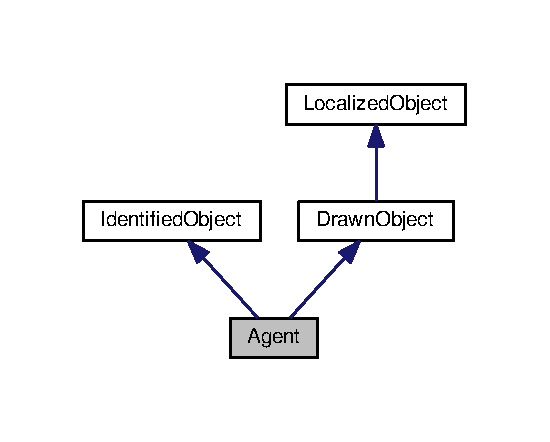
\includegraphics[width=264pt]{classAgent__inherit__graph}
\end{center}
\end{figure}


Collaboration diagram for Agent\+:\nopagebreak
\begin{figure}[H]
\begin{center}
\leavevmode
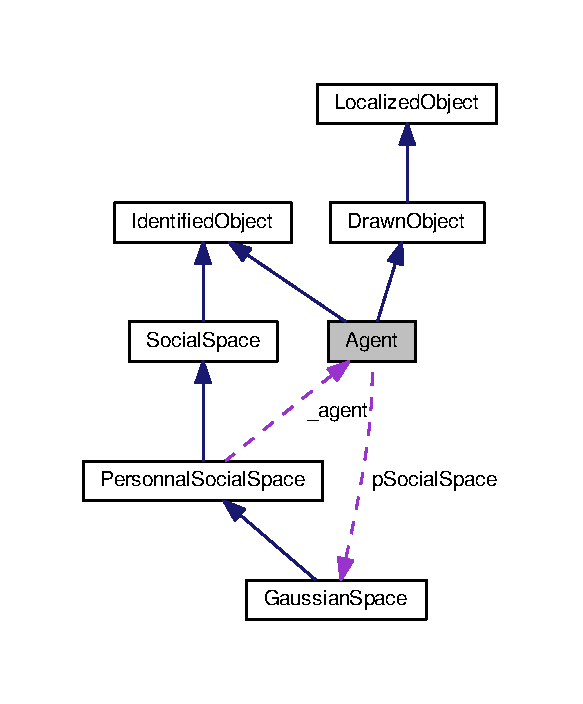
\includegraphics[width=280pt]{classAgent__coll__graph}
\end{center}
\end{figure}
\subsection*{Public Member Functions}
\begin{DoxyCompactItemize}
\item 
\hyperlink{classAgent_add6bcb014f4572bf90e489dbd35df597}{Agent} (Vector3d \hyperlink{classLocalizedObject_a340834deefc9e5c39da1f26c4ebf4f8c}{position}=Vector3d(), double \hyperlink{classLocalizedObject_aa5f7b070b6dc97a64a90797a0bca56e2}{theta}=0, int \hyperlink{classIdentifiedObject_ad044a317a9b573a3d1bcd025df166eb5}{id}=0)
\begin{DoxyCompactList}\small\item\em Constructor. \end{DoxyCompactList}\item 
\hyperlink{classAgent_ab8dd8d152605cf1339fed595376e83cb}{$\sim$\+Agent} ()
\begin{DoxyCompactList}\small\item\em Destructor. \end{DoxyCompactList}\item 
\hyperlink{classAgent}{Agent} $\ast$ \hyperlink{classAgent_a7ccfca9f14ee9d5afda1ac12effd1a33}{find\+Nearest\+Neighbor} (std\+::vector$<$ \hyperlink{classAgent}{Agent} $\ast$ $>$ agents)
\begin{DoxyCompactList}\small\item\em Find the nearest neighbor available in the list passed in parameters. \end{DoxyCompactList}\item 
Vector3d $\ast$ \hyperlink{classAgent_aef81d0795b37875777ca21d6d866ce31}{get\+F\+O\+V\+Intersection} (\hyperlink{classAgent}{Agent} $\ast$agent)
\begin{DoxyCompactList}\small\item\em Find the intersection point in the field of view with the other \hyperlink{classAgent}{Agent} passed in parameter. \end{DoxyCompactList}\item 
\hyperlink{classGaussianSpace}{Gaussian\+Space} $\ast$ \hyperlink{classAgent_aa42fced9ebe2bfec4b789ae5ed714bba}{get\+Social\+Space} () const 
\begin{DoxyCompactList}\small\item\em Simple getter. \end{DoxyCompactList}\item 
void \hyperlink{classAgent_a6b113ba7509327039373927a2e8a4e4c}{set\+Social\+Space} (\hyperlink{classGaussianSpace}{Gaussian\+Space} $\ast$social\+Space)
\begin{DoxyCompactList}\small\item\em Simple setter. \end{DoxyCompactList}\end{DoxyCompactItemize}
\subsection*{Protected Attributes}
\begin{DoxyCompactItemize}
\item 
\hyperlink{classGaussianSpace}{Gaussian\+Space} $\ast$ \hyperlink{classAgent_a4ccee7065613fc2ae660ccdf29097daa}{p\+Social\+Space}\hypertarget{classAgent_a4ccee7065613fc2ae660ccdf29097daa}{}\label{classAgent_a4ccee7065613fc2ae660ccdf29097daa}

\begin{DoxyCompactList}\small\item\em \hyperlink{classPersonnalSocialSpace}{Personnal\+Social\+Space} related to the \hyperlink{classAgent}{Agent}. \end{DoxyCompactList}\end{DoxyCompactItemize}


\subsection{Detailed Description}
This class represent the Agents. 

This class manage the Agents detected around the robot 

\subsection{Constructor \& Destructor Documentation}
\index{Agent@{Agent}!Agent@{Agent}}
\index{Agent@{Agent}!Agent@{Agent}}
\subsubsection[{\texorpdfstring{Agent(\+Vector3d position=\+Vector3d(), double theta=0, int id=0)}{Agent(Vector3d position=Vector3d(), double theta=0, int id=0)}}]{\setlength{\rightskip}{0pt plus 5cm}Agent\+::\+Agent (
\begin{DoxyParamCaption}
\item[{Vector3d}]{position = {\ttfamily Vector3d()}, }
\item[{double}]{theta = {\ttfamily 0}, }
\item[{int}]{id = {\ttfamily 0}}
\end{DoxyParamCaption}
)}\hypertarget{classAgent_add6bcb014f4572bf90e489dbd35df597}{}\label{classAgent_add6bcb014f4572bf90e489dbd35df597}


Constructor. 

Constructor of the \hyperlink{classAgent}{Agent} class, initialize a \hyperlink{classPersonnalSocialSpace}{Personnal\+Social\+Space}


\begin{DoxyParams}{Parameters}
{\em position} & \+: Initial position of the \hyperlink{classAgent}{Agent} in \hyperlink{classWorld}{World} \\
\hline
{\em theta} & \+: Initial angle of the \hyperlink{classAgent}{Agent} \\
\hline
{\em id} & \+: Unique identifier of the \hyperlink{classAgent}{Agent} \\
\hline
\end{DoxyParams}
\index{Agent@{Agent}!````~Agent@{$\sim$\+Agent}}
\index{````~Agent@{$\sim$\+Agent}!Agent@{Agent}}
\subsubsection[{\texorpdfstring{$\sim$\+Agent()}{~Agent()}}]{\setlength{\rightskip}{0pt plus 5cm}Agent\+::$\sim$\+Agent (
\begin{DoxyParamCaption}
{}
\end{DoxyParamCaption}
)}\hypertarget{classAgent_ab8dd8d152605cf1339fed595376e83cb}{}\label{classAgent_ab8dd8d152605cf1339fed595376e83cb}


Destructor. 

Destructor of the \hyperlink{classAgent}{Agent} class, destroy the related \hyperlink{classPersonnalSocialSpace}{Personnal\+Social\+Space} 

\subsection{Member Function Documentation}
\index{Agent@{Agent}!find\+Nearest\+Neighbor@{find\+Nearest\+Neighbor}}
\index{find\+Nearest\+Neighbor@{find\+Nearest\+Neighbor}!Agent@{Agent}}
\subsubsection[{\texorpdfstring{find\+Nearest\+Neighbor(std\+::vector$<$ Agent $\ast$ $>$ agents)}{findNearestNeighbor(std::vector< Agent * > agents)}}]{\setlength{\rightskip}{0pt plus 5cm}{\bf Agent} $\ast$ Agent\+::find\+Nearest\+Neighbor (
\begin{DoxyParamCaption}
\item[{std\+::vector$<$ {\bf Agent} $\ast$ $>$}]{agents}
\end{DoxyParamCaption}
)}\hypertarget{classAgent_a7ccfca9f14ee9d5afda1ac12effd1a33}{}\label{classAgent_a7ccfca9f14ee9d5afda1ac12effd1a33}


Find the nearest neighbor available in the list passed in parameters. 


\begin{DoxyParams}{Parameters}
{\em agents} & \+: A list of Agents \\
\hline
\end{DoxyParams}
\begin{DoxyReturn}{Returns}
The nearest \hyperlink{classAgent}{Agent} available in agents 
\end{DoxyReturn}
\index{Agent@{Agent}!get\+F\+O\+V\+Intersection@{get\+F\+O\+V\+Intersection}}
\index{get\+F\+O\+V\+Intersection@{get\+F\+O\+V\+Intersection}!Agent@{Agent}}
\subsubsection[{\texorpdfstring{get\+F\+O\+V\+Intersection(\+Agent $\ast$agent)}{getFOVIntersection(Agent *agent)}}]{\setlength{\rightskip}{0pt plus 5cm}Vector3d $\ast$ Agent\+::get\+F\+O\+V\+Intersection (
\begin{DoxyParamCaption}
\item[{{\bf Agent} $\ast$}]{agent}
\end{DoxyParamCaption}
)}\hypertarget{classAgent_aef81d0795b37875777ca21d6d866ce31}{}\label{classAgent_aef81d0795b37875777ca21d6d866ce31}


Find the intersection point in the field of view with the other \hyperlink{classAgent}{Agent} passed in parameter. 


\begin{DoxyParams}{Parameters}
{\em agent} & \+: The targeted \hyperlink{classAgent}{Agent} \\
\hline
\end{DoxyParams}
\begin{DoxyReturn}{Returns}
The intersection point in the field of view of both \hyperlink{classAgent}{Agent}, returns N\+U\+LL if there is no intersection
\end{DoxyReturn}
\begin{DoxyRefDesc}{Todo}
\item[\hyperlink{todo__todo000001}{Todo}]Take parallel \hyperlink{classAgent}{Agent} into account, actually return N\+U\+LL if Agents are parallel \end{DoxyRefDesc}
\index{Agent@{Agent}!get\+Social\+Space@{get\+Social\+Space}}
\index{get\+Social\+Space@{get\+Social\+Space}!Agent@{Agent}}
\subsubsection[{\texorpdfstring{get\+Social\+Space() const }{getSocialSpace() const }}]{\setlength{\rightskip}{0pt plus 5cm}{\bf Gaussian\+Space} $\ast$ Agent\+::get\+Social\+Space (
\begin{DoxyParamCaption}
{}
\end{DoxyParamCaption}
) const}\hypertarget{classAgent_aa42fced9ebe2bfec4b789ae5ed714bba}{}\label{classAgent_aa42fced9ebe2bfec4b789ae5ed714bba}


Simple getter. 

\begin{DoxyReturn}{Returns}
Personal\+Social\+Space 
\end{DoxyReturn}
\index{Agent@{Agent}!set\+Social\+Space@{set\+Social\+Space}}
\index{set\+Social\+Space@{set\+Social\+Space}!Agent@{Agent}}
\subsubsection[{\texorpdfstring{set\+Social\+Space(\+Gaussian\+Space $\ast$social\+Space)}{setSocialSpace(GaussianSpace *socialSpace)}}]{\setlength{\rightskip}{0pt plus 5cm}void Agent\+::set\+Social\+Space (
\begin{DoxyParamCaption}
\item[{{\bf Gaussian\+Space} $\ast$}]{social\+Space}
\end{DoxyParamCaption}
)}\hypertarget{classAgent_a6b113ba7509327039373927a2e8a4e4c}{}\label{classAgent_a6b113ba7509327039373927a2e8a4e4c}


Simple setter. 


\begin{DoxyParams}{Parameters}
{\em social\+Space} & \\
\hline
\end{DoxyParams}


The documentation for this class was generated from the following files\+:\begin{DoxyCompactItemize}
\item 
src/agent\+Management/\hyperlink{Agent_8h}{Agent.\+h}\item 
src/agent\+Management/\hyperlink{Agent_8cpp}{Agent.\+cpp}\end{DoxyCompactItemize}

\hypertarget{classAgentContainer}{}\section{Agent\+Container Class Reference}
\label{classAgentContainer}\index{Agent\+Container@{Agent\+Container}}


This class is an interface for class that contains multiples Agents.  




{\ttfamily \#include $<$Agent\+Container.\+h$>$}



Inheritance diagram for Agent\+Container\+:\nopagebreak
\begin{figure}[H]
\begin{center}
\leavevmode
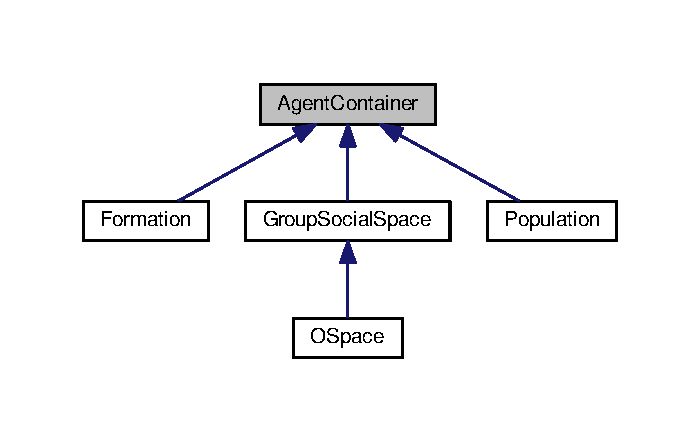
\includegraphics[width=336pt]{classAgentContainer__inherit__graph}
\end{center}
\end{figure}
\subsection*{Public Member Functions}
\begin{DoxyCompactItemize}
\item 
\hyperlink{classAgentContainer_ac7e6b1698c4270e58f6143af974b0317}{Agent\+Container} ()
\begin{DoxyCompactList}\small\item\em Constructor. \end{DoxyCompactList}\item 
\hyperlink{classAgentContainer_af38dc491d4e987a33fac7eebcbf2006b}{Agent\+Container} (std\+::vector$<$ \hyperlink{classAgent}{Agent} $\ast$ $>$ \&agents)
\begin{DoxyCompactList}\small\item\em Constructor. \end{DoxyCompactList}\item 
virtual \hyperlink{classAgentContainer_a968652639a4749f9a279fbcdf0c671e3}{$\sim$\+Agent\+Container} ()
\begin{DoxyCompactList}\small\item\em Destructor. \end{DoxyCompactList}\item 
void \hyperlink{classAgentContainer_a9fcac4f7f925326633b3d74f3923c5ff}{push\+Agent} (\hyperlink{classAgent}{Agent} $\ast$agent)
\begin{DoxyCompactList}\small\item\em Add an \hyperlink{classAgent}{Agent} to the container. \end{DoxyCompactList}\item 
int \hyperlink{classAgentContainer_a08536f977e775903573a3891a7d2f314}{remove\+Agent} (unsigned int agent\+Id)
\begin{DoxyCompactList}\small\item\em Remove an \hyperlink{classAgent}{Agent} by id from the container. \end{DoxyCompactList}\item 
void \hyperlink{classAgentContainer_a0c33290cf10b72894c245fcc298755b3}{clear\+Agents} ()
\begin{DoxyCompactList}\small\item\em Clear the container. \end{DoxyCompactList}\item 
\hyperlink{classAgent}{Agent} $\ast$ \hyperlink{classAgentContainer_a140e5a8416b3c0d4fe917641f3dc35de}{get\+Agent} (unsigned int agent\+Id)
\begin{DoxyCompactList}\small\item\em Get an \hyperlink{classAgent}{Agent} by id from the container. \end{DoxyCompactList}\item 
std\+::vector$<$ \hyperlink{classAgent}{Agent} $\ast$ $>$ \hyperlink{classAgentContainer_a9b6f87fa0c8b3ca9d49e2cff3d1c1343}{get\+Agents} ()
\begin{DoxyCompactList}\small\item\em Simple getter. \end{DoxyCompactList}\item 
void \hyperlink{classAgentContainer_a3e7b68a0539a9f4f9ba067943adfd7c1}{set\+Agents} (const std\+::vector$<$ \hyperlink{classAgent}{Agent} $\ast$ $>$ \&agents)
\begin{DoxyCompactList}\small\item\em Simple setter. \end{DoxyCompactList}\end{DoxyCompactItemize}
\subsection*{Protected Attributes}
\begin{DoxyCompactItemize}
\item 
std\+::vector$<$ \hyperlink{classAgent}{Agent} $\ast$ $>$ \hyperlink{classAgentContainer_adbcf662c5eb935864cfa02dc617e867c}{\+\_\+agents}\hypertarget{classAgentContainer_adbcf662c5eb935864cfa02dc617e867c}{}\label{classAgentContainer_adbcf662c5eb935864cfa02dc617e867c}

\begin{DoxyCompactList}\small\item\em The \hyperlink{classAgent}{Agent} container. \end{DoxyCompactList}\end{DoxyCompactItemize}


\subsection{Detailed Description}
This class is an interface for class that contains multiples Agents. 

\subsection{Constructor \& Destructor Documentation}
\index{Agent\+Container@{Agent\+Container}!Agent\+Container@{Agent\+Container}}
\index{Agent\+Container@{Agent\+Container}!Agent\+Container@{Agent\+Container}}
\subsubsection[{\texorpdfstring{Agent\+Container()}{AgentContainer()}}]{\setlength{\rightskip}{0pt plus 5cm}Agent\+Container\+::\+Agent\+Container (
\begin{DoxyParamCaption}
{}
\end{DoxyParamCaption}
)}\hypertarget{classAgentContainer_ac7e6b1698c4270e58f6143af974b0317}{}\label{classAgentContainer_ac7e6b1698c4270e58f6143af974b0317}


Constructor. 

Constructor of the \hyperlink{classAgentContainer}{Agent\+Container} class, initialize an empty container \index{Agent\+Container@{Agent\+Container}!Agent\+Container@{Agent\+Container}}
\index{Agent\+Container@{Agent\+Container}!Agent\+Container@{Agent\+Container}}
\subsubsection[{\texorpdfstring{Agent\+Container(std\+::vector$<$ Agent $\ast$ $>$ \&agents)}{AgentContainer(std::vector< Agent * > &agents)}}]{\setlength{\rightskip}{0pt plus 5cm}Agent\+Container\+::\+Agent\+Container (
\begin{DoxyParamCaption}
\item[{std\+::vector$<$ {\bf Agent} $\ast$ $>$ \&}]{agents}
\end{DoxyParamCaption}
)}\hypertarget{classAgentContainer_af38dc491d4e987a33fac7eebcbf2006b}{}\label{classAgentContainer_af38dc491d4e987a33fac7eebcbf2006b}


Constructor. 

Constructor of the \hyperlink{classAgentContainer}{Agent\+Container} class, initialize the container with agents


\begin{DoxyParams}{Parameters}
{\em agents} & \+: The Agents present in the container \\
\hline
\end{DoxyParams}
\index{Agent\+Container@{Agent\+Container}!````~Agent\+Container@{$\sim$\+Agent\+Container}}
\index{````~Agent\+Container@{$\sim$\+Agent\+Container}!Agent\+Container@{Agent\+Container}}
\subsubsection[{\texorpdfstring{$\sim$\+Agent\+Container()}{~AgentContainer()}}]{\setlength{\rightskip}{0pt plus 5cm}Agent\+Container\+::$\sim$\+Agent\+Container (
\begin{DoxyParamCaption}
{}
\end{DoxyParamCaption}
)\hspace{0.3cm}{\ttfamily [virtual]}}\hypertarget{classAgentContainer_a968652639a4749f9a279fbcdf0c671e3}{}\label{classAgentContainer_a968652639a4749f9a279fbcdf0c671e3}


Destructor. 

Destructor of the \hyperlink{classAgentContainer}{Agent\+Container} class 

\subsection{Member Function Documentation}
\index{Agent\+Container@{Agent\+Container}!clear\+Agents@{clear\+Agents}}
\index{clear\+Agents@{clear\+Agents}!Agent\+Container@{Agent\+Container}}
\subsubsection[{\texorpdfstring{clear\+Agents()}{clearAgents()}}]{\setlength{\rightskip}{0pt plus 5cm}void Agent\+Container\+::clear\+Agents (
\begin{DoxyParamCaption}
{}
\end{DoxyParamCaption}
)}\hypertarget{classAgentContainer_a0c33290cf10b72894c245fcc298755b3}{}\label{classAgentContainer_a0c33290cf10b72894c245fcc298755b3}


Clear the container. 

Clear the container, this function doesn\textquotesingle{}t call the \hyperlink{classAgent}{Agent} destructor \index{Agent\+Container@{Agent\+Container}!get\+Agent@{get\+Agent}}
\index{get\+Agent@{get\+Agent}!Agent\+Container@{Agent\+Container}}
\subsubsection[{\texorpdfstring{get\+Agent(unsigned int agent\+Id)}{getAgent(unsigned int agentId)}}]{\setlength{\rightskip}{0pt plus 5cm}{\bf Agent} $\ast$ Agent\+Container\+::get\+Agent (
\begin{DoxyParamCaption}
\item[{unsigned int}]{agent\+Id}
\end{DoxyParamCaption}
)}\hypertarget{classAgentContainer_a140e5a8416b3c0d4fe917641f3dc35de}{}\label{classAgentContainer_a140e5a8416b3c0d4fe917641f3dc35de}


Get an \hyperlink{classAgent}{Agent} by id from the container. 


\begin{DoxyParams}{Parameters}
{\em agent\+Id} & \+: \hyperlink{classAgent}{Agent} id to get from the container\\
\hline
\end{DoxyParams}
\begin{DoxyReturn}{Returns}
The \hyperlink{classAgent}{Agent}, null otherwise 
\end{DoxyReturn}
\index{Agent\+Container@{Agent\+Container}!get\+Agents@{get\+Agents}}
\index{get\+Agents@{get\+Agents}!Agent\+Container@{Agent\+Container}}
\subsubsection[{\texorpdfstring{get\+Agents()}{getAgents()}}]{\setlength{\rightskip}{0pt plus 5cm}std\+::vector$<$ {\bf Agent} $\ast$ $>$ Agent\+Container\+::get\+Agents (
\begin{DoxyParamCaption}
{}
\end{DoxyParamCaption}
)}\hypertarget{classAgentContainer_a9b6f87fa0c8b3ca9d49e2cff3d1c1343}{}\label{classAgentContainer_a9b6f87fa0c8b3ca9d49e2cff3d1c1343}


Simple getter. 

\begin{DoxyReturn}{Returns}
Agents 
\end{DoxyReturn}
\index{Agent\+Container@{Agent\+Container}!push\+Agent@{push\+Agent}}
\index{push\+Agent@{push\+Agent}!Agent\+Container@{Agent\+Container}}
\subsubsection[{\texorpdfstring{push\+Agent(\+Agent $\ast$agent)}{pushAgent(Agent *agent)}}]{\setlength{\rightskip}{0pt plus 5cm}void Agent\+Container\+::push\+Agent (
\begin{DoxyParamCaption}
\item[{{\bf Agent} $\ast$}]{agent}
\end{DoxyParamCaption}
)}\hypertarget{classAgentContainer_a9fcac4f7f925326633b3d74f3923c5ff}{}\label{classAgentContainer_a9fcac4f7f925326633b3d74f3923c5ff}


Add an \hyperlink{classAgent}{Agent} to the container. 


\begin{DoxyParams}{Parameters}
{\em agent} & \+: The \hyperlink{classAgent}{Agent} to add \\
\hline
\end{DoxyParams}
\index{Agent\+Container@{Agent\+Container}!remove\+Agent@{remove\+Agent}}
\index{remove\+Agent@{remove\+Agent}!Agent\+Container@{Agent\+Container}}
\subsubsection[{\texorpdfstring{remove\+Agent(unsigned int agent\+Id)}{removeAgent(unsigned int agentId)}}]{\setlength{\rightskip}{0pt plus 5cm}int Agent\+Container\+::remove\+Agent (
\begin{DoxyParamCaption}
\item[{unsigned int}]{agent\+Id}
\end{DoxyParamCaption}
)}\hypertarget{classAgentContainer_a08536f977e775903573a3891a7d2f314}{}\label{classAgentContainer_a08536f977e775903573a3891a7d2f314}


Remove an \hyperlink{classAgent}{Agent} by id from the container. 


\begin{DoxyParams}{Parameters}
{\em agent\+Id} & \+: The \hyperlink{classAgent}{Agent} id to remove\\
\hline
\end{DoxyParams}
\begin{DoxyReturn}{Returns}
0 on success, -\/1 if \hyperlink{classAgent}{Agent} id is not found 
\end{DoxyReturn}
\index{Agent\+Container@{Agent\+Container}!set\+Agents@{set\+Agents}}
\index{set\+Agents@{set\+Agents}!Agent\+Container@{Agent\+Container}}
\subsubsection[{\texorpdfstring{set\+Agents(const std\+::vector$<$ Agent $\ast$ $>$ \&agents)}{setAgents(const std::vector< Agent * > &agents)}}]{\setlength{\rightskip}{0pt plus 5cm}void Agent\+Container\+::set\+Agents (
\begin{DoxyParamCaption}
\item[{const std\+::vector$<$ {\bf Agent} $\ast$ $>$ \&}]{agents}
\end{DoxyParamCaption}
)}\hypertarget{classAgentContainer_a3e7b68a0539a9f4f9ba067943adfd7c1}{}\label{classAgentContainer_a3e7b68a0539a9f4f9ba067943adfd7c1}


Simple setter. 


\begin{DoxyParams}{Parameters}
{\em agents} & \\
\hline
\end{DoxyParams}


The documentation for this class was generated from the following files\+:\begin{DoxyCompactItemize}
\item 
src/generic\+Type/\hyperlink{AgentContainer_8h}{Agent\+Container.\+h}\item 
src/generic\+Type/\hyperlink{AgentContainer_8cpp}{Agent\+Container.\+cpp}\end{DoxyCompactItemize}

\hypertarget{structGridMap_1_1CompaireVCell}{}\section{Grid\+Map\+:\+:Compaire\+V\+Cell Struct Reference}
\label{structGridMap_1_1CompaireVCell}\index{Grid\+Map\+::\+Compaire\+V\+Cell@{Grid\+Map\+::\+Compaire\+V\+Cell}}


Define an operator for \hyperlink{classGridCell}{Grid\+Cell} and associated g\+Score comparison for A$\ast$ algorithm.  




{\ttfamily \#include $<$Grid\+Map.\+h$>$}

\subsection*{Public Member Functions}
\begin{DoxyCompactItemize}
\item 
bool \hyperlink{structGridMap_1_1CompaireVCell_a2d96fc322b8347479bc4cb5764c37922}{operator()} (\hyperlink{classGridMap_a3589e78d066f9c12b000f85f870afbc4}{V\+Cell} const \&a, \hyperlink{classGridMap_a3589e78d066f9c12b000f85f870afbc4}{V\+Cell} const \&b) const 
\end{DoxyCompactItemize}


\subsection{Detailed Description}
Define an operator for \hyperlink{classGridCell}{Grid\+Cell} and associated g\+Score comparison for A$\ast$ algorithm. 

\subsection{Member Function Documentation}
\index{Grid\+Map\+::\+Compaire\+V\+Cell@{Grid\+Map\+::\+Compaire\+V\+Cell}!operator()@{operator()}}
\index{operator()@{operator()}!Grid\+Map\+::\+Compaire\+V\+Cell@{Grid\+Map\+::\+Compaire\+V\+Cell}}
\subsubsection[{\texorpdfstring{operator()(\+V\+Cell const \&a, V\+Cell const \&b) const }{operator()(VCell const &a, VCell const &b) const }}]{\setlength{\rightskip}{0pt plus 5cm}bool Grid\+Map\+::\+Compaire\+V\+Cell\+::operator() (
\begin{DoxyParamCaption}
\item[{{\bf V\+Cell} const \&}]{a, }
\item[{{\bf V\+Cell} const \&}]{b}
\end{DoxyParamCaption}
) const\hspace{0.3cm}{\ttfamily [inline]}}\hypertarget{structGridMap_1_1CompaireVCell_a2d96fc322b8347479bc4cb5764c37922}{}\label{structGridMap_1_1CompaireVCell_a2d96fc322b8347479bc4cb5764c37922}

\begin{DoxyParams}{Parameters}
{\em a} & \+: The V\+Cell compared \\
\hline
{\em b} & \+: The other V\+Cell compared \\
\hline
\end{DoxyParams}
\begin{DoxyReturn}{Returns}
1 if V\+Cell have a greater score than the V\+Cell b 
\end{DoxyReturn}


The documentation for this struct was generated from the following file\+:\begin{DoxyCompactItemize}
\item 
src/world\+Representation/\hyperlink{GridMap_8h}{Grid\+Map.\+h}\end{DoxyCompactItemize}

\hypertarget{classDrawnObject}{}\section{Drawn\+Object Class Reference}
\label{classDrawnObject}\index{Drawn\+Object@{Drawn\+Object}}


This class is an interface for class that are drawn on O\+FX gui.  




{\ttfamily \#include $<$Drawn\+Object.\+h$>$}



Inheritance diagram for Drawn\+Object\+:\nopagebreak
\begin{figure}[H]
\begin{center}
\leavevmode
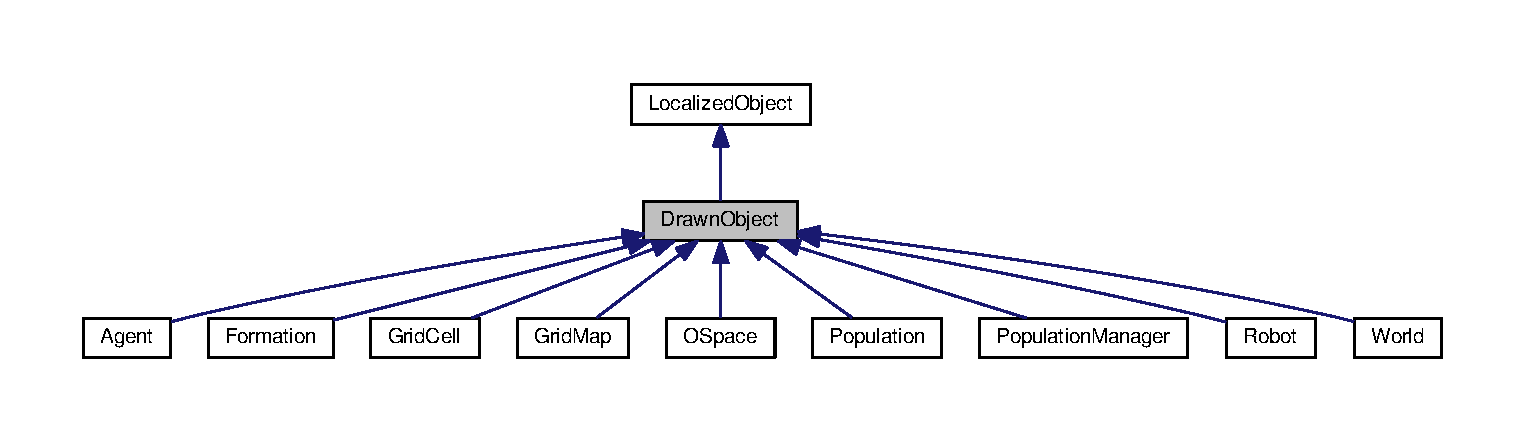
\includegraphics[width=350pt]{classDrawnObject__inherit__graph}
\end{center}
\end{figure}


Collaboration diagram for Drawn\+Object\+:\nopagebreak
\begin{figure}[H]
\begin{center}
\leavevmode
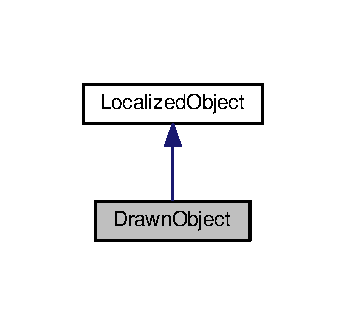
\includegraphics[width=166pt]{classDrawnObject__coll__graph}
\end{center}
\end{figure}
\subsection*{Public Member Functions}
\begin{DoxyCompactItemize}
\item 
\hyperlink{classDrawnObject_a89783864e25e1ff83cb0fc0cbf0b8ce0}{Drawn\+Object} (Vector3d \hyperlink{classLocalizedObject_a340834deefc9e5c39da1f26c4ebf4f8c}{position}=Vector3d(), double \hyperlink{classLocalizedObject_aa5f7b070b6dc97a64a90797a0bca56e2}{theta}=0)
\begin{DoxyCompactList}\small\item\em Constructor. \end{DoxyCompactList}\item 
virtual \hyperlink{classDrawnObject_ac59f1d7ad3e4d554957ff85a1f133988}{$\sim$\+Drawn\+Object} ()
\begin{DoxyCompactList}\small\item\em Destructor. \end{DoxyCompactList}\item 
Vector3d \hyperlink{classDrawnObject_a6206da4777e99b07585dcf6426ce8da6}{real\+\_\+to\+\_\+pixel} (\hyperlink{classWorld}{World} $\ast$world, Vector3d p)
\begin{DoxyCompactList}\small\item\em The projection function from real to pixel coordinates. \end{DoxyCompactList}\item 
Vector3d \hyperlink{classDrawnObject_a06f179d7fec55a350f9a78af334fa592}{pixel\+\_\+to\+\_\+real} (\hyperlink{classWorld}{World} $\ast$world, Vector3d p)
\begin{DoxyCompactList}\small\item\em The projection function from pixel to real coordinates. \end{DoxyCompactList}\end{DoxyCompactItemize}
\subsection*{Additional Inherited Members}


\subsection{Detailed Description}
This class is an interface for class that are drawn on O\+FX gui. 

\subsection{Constructor \& Destructor Documentation}
\index{Drawn\+Object@{Drawn\+Object}!Drawn\+Object@{Drawn\+Object}}
\index{Drawn\+Object@{Drawn\+Object}!Drawn\+Object@{Drawn\+Object}}
\subsubsection[{\texorpdfstring{Drawn\+Object(\+Vector3d position=\+Vector3d(), double theta=0)}{DrawnObject(Vector3d position=Vector3d(), double theta=0)}}]{\setlength{\rightskip}{0pt plus 5cm}Drawn\+Object\+::\+Drawn\+Object (
\begin{DoxyParamCaption}
\item[{Vector3d}]{position = {\ttfamily Vector3d()}, }
\item[{double}]{theta = {\ttfamily 0}}
\end{DoxyParamCaption}
)}\hypertarget{classDrawnObject_a89783864e25e1ff83cb0fc0cbf0b8ce0}{}\label{classDrawnObject_a89783864e25e1ff83cb0fc0cbf0b8ce0}


Constructor. 

Constructor of the \hyperlink{classDrawnObject}{Drawn\+Object} class


\begin{DoxyParams}{Parameters}
{\em position} & \+: The initial position of the object \\
\hline
{\em theta} & \+: The initial rotation of the object \\
\hline
\end{DoxyParams}
\index{Drawn\+Object@{Drawn\+Object}!````~Drawn\+Object@{$\sim$\+Drawn\+Object}}
\index{````~Drawn\+Object@{$\sim$\+Drawn\+Object}!Drawn\+Object@{Drawn\+Object}}
\subsubsection[{\texorpdfstring{$\sim$\+Drawn\+Object()}{~DrawnObject()}}]{\setlength{\rightskip}{0pt plus 5cm}Drawn\+Object\+::$\sim$\+Drawn\+Object (
\begin{DoxyParamCaption}
{}
\end{DoxyParamCaption}
)\hspace{0.3cm}{\ttfamily [virtual]}}\hypertarget{classDrawnObject_ac59f1d7ad3e4d554957ff85a1f133988}{}\label{classDrawnObject_ac59f1d7ad3e4d554957ff85a1f133988}


Destructor. 

Destructor of the \hyperlink{classDrawnObject}{Drawn\+Object} class 

\subsection{Member Function Documentation}
\index{Drawn\+Object@{Drawn\+Object}!pixel\+\_\+to\+\_\+real@{pixel\+\_\+to\+\_\+real}}
\index{pixel\+\_\+to\+\_\+real@{pixel\+\_\+to\+\_\+real}!Drawn\+Object@{Drawn\+Object}}
\subsubsection[{\texorpdfstring{pixel\+\_\+to\+\_\+real(\+World $\ast$world, Vector3d p)}{pixel_to_real(World *world, Vector3d p)}}]{\setlength{\rightskip}{0pt plus 5cm}Vector3d Drawn\+Object\+::pixel\+\_\+to\+\_\+real (
\begin{DoxyParamCaption}
\item[{{\bf World} $\ast$}]{world, }
\item[{Vector3d}]{p}
\end{DoxyParamCaption}
)}\hypertarget{classDrawnObject_a06f179d7fec55a350f9a78af334fa592}{}\label{classDrawnObject_a06f179d7fec55a350f9a78af334fa592}


The projection function from pixel to real coordinates. 


\begin{DoxyParams}{Parameters}
{\em world} & \+: The \hyperlink{classWorld}{World} main coordinates frame \\
\hline
{\em p} & \+: The vector that will be projected\\
\hline
\end{DoxyParams}
\begin{DoxyReturn}{Returns}
The projected vector in real coordinates 
\end{DoxyReturn}
\index{Drawn\+Object@{Drawn\+Object}!real\+\_\+to\+\_\+pixel@{real\+\_\+to\+\_\+pixel}}
\index{real\+\_\+to\+\_\+pixel@{real\+\_\+to\+\_\+pixel}!Drawn\+Object@{Drawn\+Object}}
\subsubsection[{\texorpdfstring{real\+\_\+to\+\_\+pixel(\+World $\ast$world, Vector3d p)}{real_to_pixel(World *world, Vector3d p)}}]{\setlength{\rightskip}{0pt plus 5cm}Vector3d Drawn\+Object\+::real\+\_\+to\+\_\+pixel (
\begin{DoxyParamCaption}
\item[{{\bf World} $\ast$}]{world, }
\item[{Vector3d}]{p}
\end{DoxyParamCaption}
)}\hypertarget{classDrawnObject_a6206da4777e99b07585dcf6426ce8da6}{}\label{classDrawnObject_a6206da4777e99b07585dcf6426ce8da6}


The projection function from real to pixel coordinates. 


\begin{DoxyParams}{Parameters}
{\em world} & \+: The \hyperlink{classWorld}{World} main coordinates frame \\
\hline
{\em p} & \+: The vector that will be projected\\
\hline
\end{DoxyParams}
\begin{DoxyReturn}{Returns}
The projected vector in pixel coordinates 
\end{DoxyReturn}


The documentation for this class was generated from the following files\+:\begin{DoxyCompactItemize}
\item 
src/generic\+Type/\hyperlink{DrawnObject_8h}{Drawn\+Object.\+h}\item 
src/generic\+Type/\hyperlink{DrawnObject_8cpp}{Drawn\+Object.\+cpp}\end{DoxyCompactItemize}

\hypertarget{classFormation}{}\section{Formation Class Reference}
\label{classFormation}\index{Formation@{Formation}}


This class represent the social \hyperlink{classFormation}{Formation}.  




{\ttfamily \#include $<$Formation.\+h$>$}



Inheritance diagram for Formation\+:\nopagebreak
\begin{figure}[H]
\begin{center}
\leavevmode
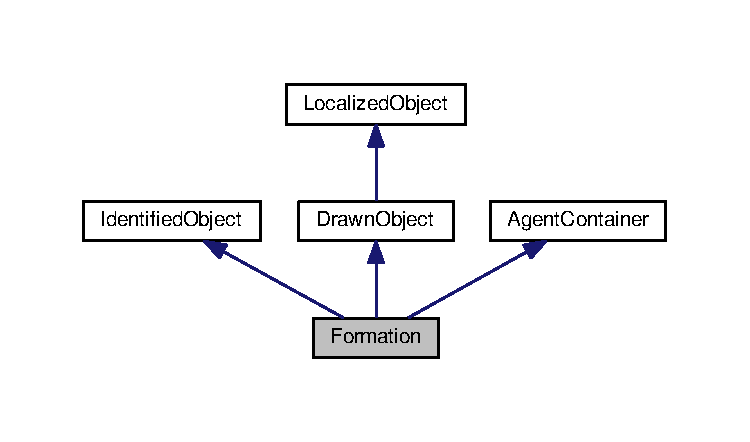
\includegraphics[width=350pt]{classFormation__inherit__graph}
\end{center}
\end{figure}


Collaboration diagram for Formation\+:\nopagebreak
\begin{figure}[H]
\begin{center}
\leavevmode
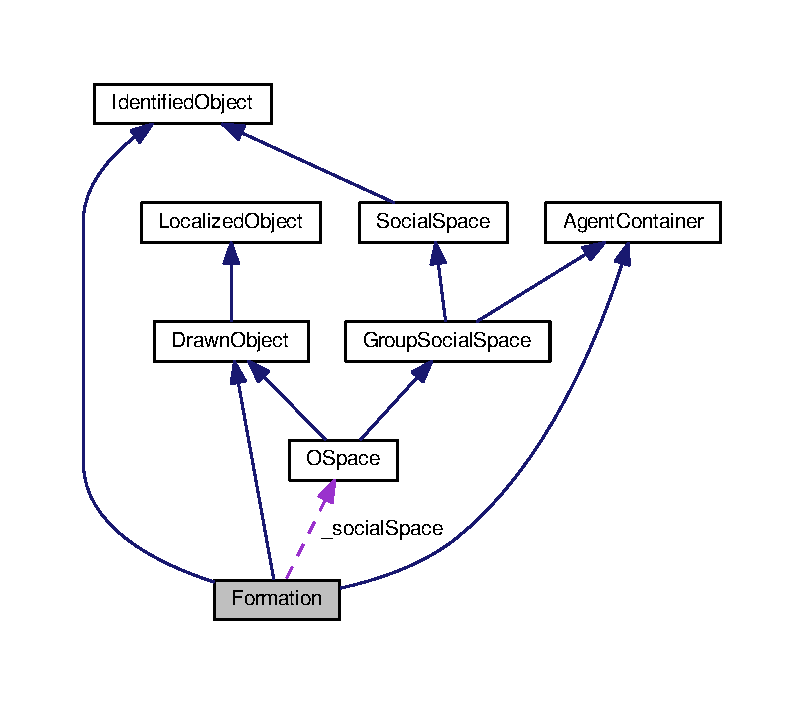
\includegraphics[width=350pt]{classFormation__coll__graph}
\end{center}
\end{figure}
\subsection*{Public Member Functions}
\begin{DoxyCompactItemize}
\item 
\hyperlink{classFormation_a5ec34c4941defd2b033f1f03bb42671f}{Formation} (std\+::vector$<$ \hyperlink{classAgent}{Agent} $\ast$ $>$ agents, int \hyperlink{classIdentifiedObject_ad044a317a9b573a3d1bcd025df166eb5}{id}=0)
\begin{DoxyCompactList}\small\item\em Constructor. \end{DoxyCompactList}\item 
\hyperlink{classFormation_a9c1013f55ac92dc20a81abc47c7849f2}{Formation} (\hyperlink{classAgent}{Agent} $\ast$agent, int \hyperlink{classIdentifiedObject_ad044a317a9b573a3d1bcd025df166eb5}{id}=0)
\begin{DoxyCompactList}\small\item\em Constructor. \end{DoxyCompactList}\item 
\hyperlink{classFormation_a7e1681f1a7b0e540f3c011179d5e8f12}{Formation} (int \hyperlink{classIdentifiedObject_ad044a317a9b573a3d1bcd025df166eb5}{id}=0)
\begin{DoxyCompactList}\small\item\em Constructor. \end{DoxyCompactList}\item 
\hyperlink{classFormation_a5b4ffd37549ec211d85e52c916f35eb6}{$\sim$\+Formation} ()
\begin{DoxyCompactList}\small\item\em Destructor. \end{DoxyCompactList}\item 
void \hyperlink{classFormation_aaa8469c44391f3255feca75d8d5d4ccc}{compute\+Interaction\+Potential} ()\hypertarget{classFormation_aaa8469c44391f3255feca75d8d5d4ccc}{}\label{classFormation_aaa8469c44391f3255feca75d8d5d4ccc}

\begin{DoxyCompactList}\small\item\em Compute the interaction potential of the formation based on the mean interpersonal distance and distance from the \hyperlink{classFormation}{Formation} center. \end{DoxyCompactList}\item 
void \hyperlink{classFormation_a5fd3207fbc27069771949e48c6fed283}{find\+Interaction\+Position} ()\hypertarget{classFormation_a5fd3207fbc27069771949e48c6fed283}{}\label{classFormation_a5fd3207fbc27069771949e48c6fed283}

\begin{DoxyCompactList}\small\item\em Compute the interaction position from the robot to adopt in order to take part in the \hyperlink{classFormation}{Formation}. \end{DoxyCompactList}\item 
void \hyperlink{classFormation_a0d340a1151f9bbcf85082da48adddd58}{update} ()\hypertarget{classFormation_a0d340a1151f9bbcf85082da48adddd58}{}\label{classFormation_a0d340a1151f9bbcf85082da48adddd58}

\begin{DoxyCompactList}\small\item\em Update \hyperlink{classFormation}{Formation} related data by calling \hyperlink{classGroupSocialSpace}{Group\+Social\+Space} update function, compute\+Interaction\+Potential and find\+Interaction\+Position. \end{DoxyCompactList}\item 
void \hyperlink{classFormation_a76796be1ec2e264b90011139bfb0347b}{push\+Agent} (\hyperlink{classAgent}{Agent} $\ast$agent)
\begin{DoxyCompactList}\small\item\em Add an \hyperlink{classAgent}{Agent} to the \hyperlink{classFormation}{Formation} and update/create the corresponding \hyperlink{classGroupSocialSpace}{Group\+Social\+Space}. \end{DoxyCompactList}\item 
void \hyperlink{classFormation_acabd4b08ca629208eca4db572360a0ab}{remove\+Agent} (unsigned int agent\+Id)
\begin{DoxyCompactList}\small\item\em Remove an \hyperlink{classAgent}{Agent} by id from the \hyperlink{classFormation}{Formation} and the corresponding \hyperlink{classGroupSocialSpace}{Group\+Social\+Space}. \end{DoxyCompactList}\item 
int \hyperlink{classFormation_a20c4f00445b98ddf0f70ffeca020dba4}{is\+In\+Formation} (\hyperlink{classAgent}{Agent} $\ast$agent)
\begin{DoxyCompactList}\small\item\em Check if the \hyperlink{classAgent}{Agent} passed in parameter is taking part in the \hyperlink{classFormation}{Formation} Alias to is\+In\+Formation function by \hyperlink{classAgent}{Agent} id. \end{DoxyCompactList}\item 
int \hyperlink{classFormation_ae8b0264d952409f51306a85463cfc2e2}{is\+In\+Formation} (unsigned int agent\+Id)
\begin{DoxyCompactList}\small\item\em Check if the \hyperlink{classAgent}{Agent} passed in parameter is taking part in the \hyperlink{classFormation}{Formation}. \end{DoxyCompactList}\item 
std\+::vector$<$ \hyperlink{classAgent}{Agent} $\ast$ $>$ \hyperlink{classFormation_aaa0230f1b5c293a654da7bea95f0f840}{init\+Agent} (\hyperlink{classAgent}{Agent} $\ast$agent)
\begin{DoxyCompactList}\small\item\em Initialization function for \hyperlink{classFormation}{Formation} Constructor with only one \hyperlink{classAgent}{Agent}. \end{DoxyCompactList}\item 
\hyperlink{classOSpace}{O\+Space} $\ast$ \hyperlink{classFormation_a51d07ac063aa2897f2c756dfea14ff5e}{get\+Social\+Space} () const 
\begin{DoxyCompactList}\small\item\em Simple getter. \end{DoxyCompactList}\item 
void \hyperlink{classFormation_a4bb19bf1b792b5a909735160408216bf}{set\+Social\+Space} (\hyperlink{classOSpace}{O\+Space} $\ast$social\+Space)
\begin{DoxyCompactList}\small\item\em Simple setter. \end{DoxyCompactList}\item 
double \hyperlink{classFormation_a1e7f7add3878012188316df803ce5677}{get\+Interaction\+Potential} () const 
\begin{DoxyCompactList}\small\item\em Simple getter. \end{DoxyCompactList}\item 
void \hyperlink{classFormation_aeae0835beea6e8544837438d58bb6582}{set\+Interaction\+Potential} (double \hyperlink{classFormation_afac1af6d51a6b8a910df4574cb7a6931}{interaction\+Potential}=0)
\begin{DoxyCompactList}\small\item\em Simple setter. \end{DoxyCompactList}\item 
const Vector3d \& \hyperlink{classFormation_af6cf9389675ea316079ef643f55ffaae}{get\+Interaction\+Position} () const 
\begin{DoxyCompactList}\small\item\em Simple getter. \end{DoxyCompactList}\item 
void \hyperlink{classFormation_a36cb4fa3ae4e3e6f761a2d1f8bb54ccb}{set\+Interaction\+Position} (const Vector3d \&\hyperlink{classFormation_a5e33d98c2b9ec916e601ae27d6c7f2ef}{interaction\+Position})
\begin{DoxyCompactList}\small\item\em Simpler setter. \end{DoxyCompactList}\item 
const Vector3d \& \hyperlink{classFormation_aa7b5cef840f4d1faefa49ef27e72c8f9}{get\+Interaction\+Direction} () const 
\begin{DoxyCompactList}\small\item\em Simpler getter. \end{DoxyCompactList}\item 
void \hyperlink{classFormation_a96fd57ec8928cc70628e0732500dd833}{set\+Interaction\+Direction} (const Vector3d \&\hyperlink{classFormation_aa68570fc8c85c172fadaf93d30367371}{interaction\+Direction})
\begin{DoxyCompactList}\small\item\em Simple setter. \end{DoxyCompactList}\end{DoxyCompactItemize}
\subsection*{Protected Attributes}
\begin{DoxyCompactItemize}
\item 
\hyperlink{classOSpace}{O\+Space} $\ast$ \hyperlink{classFormation_a8d69dd518359bf8d1d1b30a5c07db561}{\+\_\+social\+Space}\hypertarget{classFormation_a8d69dd518359bf8d1d1b30a5c07db561}{}\label{classFormation_a8d69dd518359bf8d1d1b30a5c07db561}

\begin{DoxyCompactList}\small\item\em \hyperlink{classGroupSocialSpace}{Group\+Social\+Space} related to the \hyperlink{classFormation}{Formation}. \end{DoxyCompactList}\item 
double \hyperlink{classFormation_afac1af6d51a6b8a910df4574cb7a6931}{interaction\+Potential} = 0\hypertarget{classFormation_afac1af6d51a6b8a910df4574cb7a6931}{}\label{classFormation_afac1af6d51a6b8a910df4574cb7a6931}

\begin{DoxyCompactList}\small\item\em Estimated interaction potential of the \hyperlink{classFormation}{Formation}. \end{DoxyCompactList}\item 
Vector3d \hyperlink{classFormation_a5e33d98c2b9ec916e601ae27d6c7f2ef}{interaction\+Position}\hypertarget{classFormation_a5e33d98c2b9ec916e601ae27d6c7f2ef}{}\label{classFormation_a5e33d98c2b9ec916e601ae27d6c7f2ef}

\begin{DoxyCompactList}\small\item\em Estimated interaction position for the \hyperlink{classRobot}{Robot} to take part in the \hyperlink{classFormation}{Formation}. \end{DoxyCompactList}\item 
Vector3d \hyperlink{classFormation_aa68570fc8c85c172fadaf93d30367371}{interaction\+Direction}\hypertarget{classFormation_aa68570fc8c85c172fadaf93d30367371}{}\label{classFormation_aa68570fc8c85c172fadaf93d30367371}

\begin{DoxyCompactList}\small\item\em Estimated interaction direction for the \hyperlink{classRobot}{Robot} to take part in the \hyperlink{classFormation}{Formation}. \end{DoxyCompactList}\item 
std\+::vector$<$ Vector3d $>$ \hyperlink{classFormation_a666d230b80d3d019b60beb287770be26}{agent\+Dir\+\_\+ospace}\hypertarget{classFormation_a666d230b80d3d019b60beb287770be26}{}\label{classFormation_a666d230b80d3d019b60beb287770be26}

\begin{DoxyCompactList}\small\item\em Vector3d of Agents direction to the \hyperlink{classFormation}{Formation} center. \end{DoxyCompactList}\end{DoxyCompactItemize}


\subsection{Detailed Description}
This class represent the social \hyperlink{classFormation}{Formation}. 

This class manage the social Formations created by the Agents 

\subsection{Constructor \& Destructor Documentation}
\index{Formation@{Formation}!Formation@{Formation}}
\index{Formation@{Formation}!Formation@{Formation}}
\subsubsection[{\texorpdfstring{Formation(std\+::vector$<$ Agent $\ast$ $>$ agents, int id=0)}{Formation(std::vector< Agent * > agents, int id=0)}}]{\setlength{\rightskip}{0pt plus 5cm}Formation\+::\+Formation (
\begin{DoxyParamCaption}
\item[{std\+::vector$<$ {\bf Agent} $\ast$ $>$}]{agents, }
\item[{int}]{id = {\ttfamily 0}}
\end{DoxyParamCaption}
)}\hypertarget{classFormation_a5ec34c4941defd2b033f1f03bb42671f}{}\label{classFormation_a5ec34c4941defd2b033f1f03bb42671f}


Constructor. 

Constructor of the \hyperlink{classFormation}{Formation} class, initialize a \hyperlink{classGroupSocialSpace}{Group\+Social\+Space}


\begin{DoxyParams}{Parameters}
{\em agents} & \+: Agents that are part of the \hyperlink{classFormation}{Formation} \\
\hline
{\em id} & \+: Unique identifier of the \hyperlink{classFormation}{Formation} \\
\hline
\end{DoxyParams}
\index{Formation@{Formation}!Formation@{Formation}}
\index{Formation@{Formation}!Formation@{Formation}}
\subsubsection[{\texorpdfstring{Formation(\+Agent $\ast$agent, int id=0)}{Formation(Agent *agent, int id=0)}}]{\setlength{\rightskip}{0pt plus 5cm}Formation\+::\+Formation (
\begin{DoxyParamCaption}
\item[{{\bf Agent} $\ast$}]{agent, }
\item[{int}]{id = {\ttfamily 0}}
\end{DoxyParamCaption}
)}\hypertarget{classFormation_a9c1013f55ac92dc20a81abc47c7849f2}{}\label{classFormation_a9c1013f55ac92dc20a81abc47c7849f2}


Constructor. 

Constructor of the \hyperlink{classFormation}{Formation} class, this constructor doesn\textquotesingle{}t initialize any \hyperlink{classGroupSocialSpace}{Group\+Social\+Space}


\begin{DoxyParams}{Parameters}
{\em agent} & \+: \hyperlink{classAgent}{Agent} that is part of the \hyperlink{classFormation}{Formation} \\
\hline
{\em id} & \+: Unique identifier of the \hyperlink{classFormation}{Formation} \\
\hline
\end{DoxyParams}
\index{Formation@{Formation}!Formation@{Formation}}
\index{Formation@{Formation}!Formation@{Formation}}
\subsubsection[{\texorpdfstring{Formation(int id=0)}{Formation(int id=0)}}]{\setlength{\rightskip}{0pt plus 5cm}Formation\+::\+Formation (
\begin{DoxyParamCaption}
\item[{int}]{id = {\ttfamily 0}}
\end{DoxyParamCaption}
)}\hypertarget{classFormation_a7e1681f1a7b0e540f3c011179d5e8f12}{}\label{classFormation_a7e1681f1a7b0e540f3c011179d5e8f12}


Constructor. 

Constructor of the \hyperlink{classFormation}{Formation} class, creates an empty formation. This constructor doesn\textquotesingle{}t initialize any \hyperlink{classGroupSocialSpace}{Group\+Social\+Space}


\begin{DoxyParams}{Parameters}
{\em id} & \+: Unique identifier of the \hyperlink{classFormation}{Formation} \\
\hline
\end{DoxyParams}
\index{Formation@{Formation}!````~Formation@{$\sim$\+Formation}}
\index{````~Formation@{$\sim$\+Formation}!Formation@{Formation}}
\subsubsection[{\texorpdfstring{$\sim$\+Formation()}{~Formation()}}]{\setlength{\rightskip}{0pt plus 5cm}Formation\+::$\sim$\+Formation (
\begin{DoxyParamCaption}
{}
\end{DoxyParamCaption}
)}\hypertarget{classFormation_a5b4ffd37549ec211d85e52c916f35eb6}{}\label{classFormation_a5b4ffd37549ec211d85e52c916f35eb6}


Destructor. 

Destructor of the \hyperlink{classFormation}{Formation} class, destroy the related \hyperlink{classGroupSocialSpace}{Group\+Social\+Space} if defined 

\subsection{Member Function Documentation}
\index{Formation@{Formation}!get\+Interaction\+Direction@{get\+Interaction\+Direction}}
\index{get\+Interaction\+Direction@{get\+Interaction\+Direction}!Formation@{Formation}}
\subsubsection[{\texorpdfstring{get\+Interaction\+Direction() const }{getInteractionDirection() const }}]{\setlength{\rightskip}{0pt plus 5cm}const Vector3d \& Formation\+::get\+Interaction\+Direction (
\begin{DoxyParamCaption}
{}
\end{DoxyParamCaption}
) const}\hypertarget{classFormation_aa7b5cef840f4d1faefa49ef27e72c8f9}{}\label{classFormation_aa7b5cef840f4d1faefa49ef27e72c8f9}


Simpler getter. 

\begin{DoxyReturn}{Returns}
Interaction\+Direction 
\end{DoxyReturn}
\index{Formation@{Formation}!get\+Interaction\+Position@{get\+Interaction\+Position}}
\index{get\+Interaction\+Position@{get\+Interaction\+Position}!Formation@{Formation}}
\subsubsection[{\texorpdfstring{get\+Interaction\+Position() const }{getInteractionPosition() const }}]{\setlength{\rightskip}{0pt plus 5cm}const Vector3d \& Formation\+::get\+Interaction\+Position (
\begin{DoxyParamCaption}
{}
\end{DoxyParamCaption}
) const}\hypertarget{classFormation_af6cf9389675ea316079ef643f55ffaae}{}\label{classFormation_af6cf9389675ea316079ef643f55ffaae}


Simple getter. 

\begin{DoxyReturn}{Returns}
Interaction\+Position 
\end{DoxyReturn}
\index{Formation@{Formation}!get\+Interaction\+Potential@{get\+Interaction\+Potential}}
\index{get\+Interaction\+Potential@{get\+Interaction\+Potential}!Formation@{Formation}}
\subsubsection[{\texorpdfstring{get\+Interaction\+Potential() const }{getInteractionPotential() const }}]{\setlength{\rightskip}{0pt plus 5cm}double Formation\+::get\+Interaction\+Potential (
\begin{DoxyParamCaption}
{}
\end{DoxyParamCaption}
) const}\hypertarget{classFormation_a1e7f7add3878012188316df803ce5677}{}\label{classFormation_a1e7f7add3878012188316df803ce5677}


Simple getter. 

\begin{DoxyReturn}{Returns}
Interaction\+Potential 
\end{DoxyReturn}
\index{Formation@{Formation}!get\+Social\+Space@{get\+Social\+Space}}
\index{get\+Social\+Space@{get\+Social\+Space}!Formation@{Formation}}
\subsubsection[{\texorpdfstring{get\+Social\+Space() const }{getSocialSpace() const }}]{\setlength{\rightskip}{0pt plus 5cm}{\bf O\+Space} $\ast$ Formation\+::get\+Social\+Space (
\begin{DoxyParamCaption}
{}
\end{DoxyParamCaption}
) const}\hypertarget{classFormation_a51d07ac063aa2897f2c756dfea14ff5e}{}\label{classFormation_a51d07ac063aa2897f2c756dfea14ff5e}


Simple getter. 

\begin{DoxyReturn}{Returns}
\hyperlink{classGroupSocialSpace}{Group\+Social\+Space} 
\end{DoxyReturn}
\index{Formation@{Formation}!init\+Agent@{init\+Agent}}
\index{init\+Agent@{init\+Agent}!Formation@{Formation}}
\subsubsection[{\texorpdfstring{init\+Agent(\+Agent $\ast$agent)}{initAgent(Agent *agent)}}]{\setlength{\rightskip}{0pt plus 5cm}std\+::vector$<$ {\bf Agent} $\ast$ $>$ Formation\+::init\+Agent (
\begin{DoxyParamCaption}
\item[{{\bf Agent} $\ast$}]{agent}
\end{DoxyParamCaption}
)}\hypertarget{classFormation_aaa0230f1b5c293a654da7bea95f0f840}{}\label{classFormation_aaa0230f1b5c293a654da7bea95f0f840}


Initialization function for \hyperlink{classFormation}{Formation} Constructor with only one \hyperlink{classAgent}{Agent}. 


\begin{DoxyParams}{Parameters}
{\em agent} & \+: \hyperlink{classAgent}{Agent} initialized for the \hyperlink{classFormation}{Formation}\\
\hline
\end{DoxyParams}
\begin{DoxyReturn}{Returns}
A vector containing the \hyperlink{classAgent}{Agent} passed in parameter. 
\end{DoxyReturn}
\index{Formation@{Formation}!is\+In\+Formation@{is\+In\+Formation}}
\index{is\+In\+Formation@{is\+In\+Formation}!Formation@{Formation}}
\subsubsection[{\texorpdfstring{is\+In\+Formation(\+Agent $\ast$agent)}{isInFormation(Agent *agent)}}]{\setlength{\rightskip}{0pt plus 5cm}int Formation\+::is\+In\+Formation (
\begin{DoxyParamCaption}
\item[{{\bf Agent} $\ast$}]{agent}
\end{DoxyParamCaption}
)}\hypertarget{classFormation_a20c4f00445b98ddf0f70ffeca020dba4}{}\label{classFormation_a20c4f00445b98ddf0f70ffeca020dba4}


Check if the \hyperlink{classAgent}{Agent} passed in parameter is taking part in the \hyperlink{classFormation}{Formation} Alias to is\+In\+Formation function by \hyperlink{classAgent}{Agent} id. 


\begin{DoxyParams}{Parameters}
{\em agent} & \+: \hyperlink{classAgent}{Agent} pointer to check\\
\hline
\end{DoxyParams}
\begin{DoxyReturn}{Returns}
1 if the \hyperlink{classAgent}{Agent} is taking part in the \hyperlink{classFormation}{Formation}, 0 otherwise 
\end{DoxyReturn}
\index{Formation@{Formation}!is\+In\+Formation@{is\+In\+Formation}}
\index{is\+In\+Formation@{is\+In\+Formation}!Formation@{Formation}}
\subsubsection[{\texorpdfstring{is\+In\+Formation(unsigned int agent\+Id)}{isInFormation(unsigned int agentId)}}]{\setlength{\rightskip}{0pt plus 5cm}int Formation\+::is\+In\+Formation (
\begin{DoxyParamCaption}
\item[{unsigned int}]{agent\+Id}
\end{DoxyParamCaption}
)}\hypertarget{classFormation_ae8b0264d952409f51306a85463cfc2e2}{}\label{classFormation_ae8b0264d952409f51306a85463cfc2e2}


Check if the \hyperlink{classAgent}{Agent} passed in parameter is taking part in the \hyperlink{classFormation}{Formation}. 


\begin{DoxyParams}{Parameters}
{\em agent\+Id} & \+: \hyperlink{classAgent}{Agent} id to check\\
\hline
\end{DoxyParams}
\begin{DoxyReturn}{Returns}
1 if the \hyperlink{classAgent}{Agent} is taking part in the \hyperlink{classFormation}{Formation}, 0 otherwise 
\end{DoxyReturn}
\index{Formation@{Formation}!push\+Agent@{push\+Agent}}
\index{push\+Agent@{push\+Agent}!Formation@{Formation}}
\subsubsection[{\texorpdfstring{push\+Agent(\+Agent $\ast$agent)}{pushAgent(Agent *agent)}}]{\setlength{\rightskip}{0pt plus 5cm}void Formation\+::push\+Agent (
\begin{DoxyParamCaption}
\item[{{\bf Agent} $\ast$}]{agent}
\end{DoxyParamCaption}
)}\hypertarget{classFormation_a76796be1ec2e264b90011139bfb0347b}{}\label{classFormation_a76796be1ec2e264b90011139bfb0347b}


Add an \hyperlink{classAgent}{Agent} to the \hyperlink{classFormation}{Formation} and update/create the corresponding \hyperlink{classGroupSocialSpace}{Group\+Social\+Space}. 


\begin{DoxyParams}{Parameters}
{\em agent} & \+: \hyperlink{classAgent}{Agent} pointer to add to the formation \\
\hline
\end{DoxyParams}
\index{Formation@{Formation}!remove\+Agent@{remove\+Agent}}
\index{remove\+Agent@{remove\+Agent}!Formation@{Formation}}
\subsubsection[{\texorpdfstring{remove\+Agent(unsigned int agent\+Id)}{removeAgent(unsigned int agentId)}}]{\setlength{\rightskip}{0pt plus 5cm}void Formation\+::remove\+Agent (
\begin{DoxyParamCaption}
\item[{unsigned int}]{agent\+Id}
\end{DoxyParamCaption}
)}\hypertarget{classFormation_acabd4b08ca629208eca4db572360a0ab}{}\label{classFormation_acabd4b08ca629208eca4db572360a0ab}


Remove an \hyperlink{classAgent}{Agent} by id from the \hyperlink{classFormation}{Formation} and the corresponding \hyperlink{classGroupSocialSpace}{Group\+Social\+Space}. 


\begin{DoxyParams}{Parameters}
{\em agent\+Id} & \+: \hyperlink{classAgent}{Agent} id to remove from the \hyperlink{classFormation}{Formation} \\
\hline
\end{DoxyParams}
\index{Formation@{Formation}!set\+Interaction\+Direction@{set\+Interaction\+Direction}}
\index{set\+Interaction\+Direction@{set\+Interaction\+Direction}!Formation@{Formation}}
\subsubsection[{\texorpdfstring{set\+Interaction\+Direction(const Vector3d \&interaction\+Direction)}{setInteractionDirection(const Vector3d &interactionDirection)}}]{\setlength{\rightskip}{0pt plus 5cm}void Formation\+::set\+Interaction\+Direction (
\begin{DoxyParamCaption}
\item[{const Vector3d \&}]{interaction\+Direction}
\end{DoxyParamCaption}
)}\hypertarget{classFormation_a96fd57ec8928cc70628e0732500dd833}{}\label{classFormation_a96fd57ec8928cc70628e0732500dd833}


Simple setter. 


\begin{DoxyParams}{Parameters}
{\em interaction\+Direction} & \\
\hline
\end{DoxyParams}
\index{Formation@{Formation}!set\+Interaction\+Position@{set\+Interaction\+Position}}
\index{set\+Interaction\+Position@{set\+Interaction\+Position}!Formation@{Formation}}
\subsubsection[{\texorpdfstring{set\+Interaction\+Position(const Vector3d \&interaction\+Position)}{setInteractionPosition(const Vector3d &interactionPosition)}}]{\setlength{\rightskip}{0pt plus 5cm}void Formation\+::set\+Interaction\+Position (
\begin{DoxyParamCaption}
\item[{const Vector3d \&}]{interaction\+Position}
\end{DoxyParamCaption}
)}\hypertarget{classFormation_a36cb4fa3ae4e3e6f761a2d1f8bb54ccb}{}\label{classFormation_a36cb4fa3ae4e3e6f761a2d1f8bb54ccb}


Simpler setter. 


\begin{DoxyParams}{Parameters}
{\em interaction\+Position} & \\
\hline
\end{DoxyParams}
\index{Formation@{Formation}!set\+Interaction\+Potential@{set\+Interaction\+Potential}}
\index{set\+Interaction\+Potential@{set\+Interaction\+Potential}!Formation@{Formation}}
\subsubsection[{\texorpdfstring{set\+Interaction\+Potential(double interaction\+Potential=0)}{setInteractionPotential(double interactionPotential=0)}}]{\setlength{\rightskip}{0pt plus 5cm}void Formation\+::set\+Interaction\+Potential (
\begin{DoxyParamCaption}
\item[{double}]{interaction\+Potential = {\ttfamily 0}}
\end{DoxyParamCaption}
)}\hypertarget{classFormation_aeae0835beea6e8544837438d58bb6582}{}\label{classFormation_aeae0835beea6e8544837438d58bb6582}


Simple setter. 


\begin{DoxyParams}{Parameters}
{\em interaction\+Potential} & \\
\hline
\end{DoxyParams}
\index{Formation@{Formation}!set\+Social\+Space@{set\+Social\+Space}}
\index{set\+Social\+Space@{set\+Social\+Space}!Formation@{Formation}}
\subsubsection[{\texorpdfstring{set\+Social\+Space(\+O\+Space $\ast$social\+Space)}{setSocialSpace(OSpace *socialSpace)}}]{\setlength{\rightskip}{0pt plus 5cm}void Formation\+::set\+Social\+Space (
\begin{DoxyParamCaption}
\item[{{\bf O\+Space} $\ast$}]{social\+Space}
\end{DoxyParamCaption}
)}\hypertarget{classFormation_a4bb19bf1b792b5a909735160408216bf}{}\label{classFormation_a4bb19bf1b792b5a909735160408216bf}


Simple setter. 


\begin{DoxyParams}{Parameters}
{\em social\+Space} & \\
\hline
\end{DoxyParams}


The documentation for this class was generated from the following files\+:\begin{DoxyCompactItemize}
\item 
src/agent\+Management/\hyperlink{Formation_8h}{Formation.\+h}\item 
src/agent\+Management/\hyperlink{Formation_8cpp}{Formation.\+cpp}\end{DoxyCompactItemize}

\hypertarget{classGaussianSpace}{}\section{Gaussian\+Space Class Reference}
\label{classGaussianSpace}\index{Gaussian\+Space@{Gaussian\+Space}}


This class is an implementation of the \hyperlink{classPersonnalSocialSpace}{Personnal\+Social\+Space}.  




{\ttfamily \#include $<$Gaussian\+Space.\+h$>$}



Inheritance diagram for Gaussian\+Space\+:\nopagebreak
\begin{figure}[H]
\begin{center}
\leavevmode
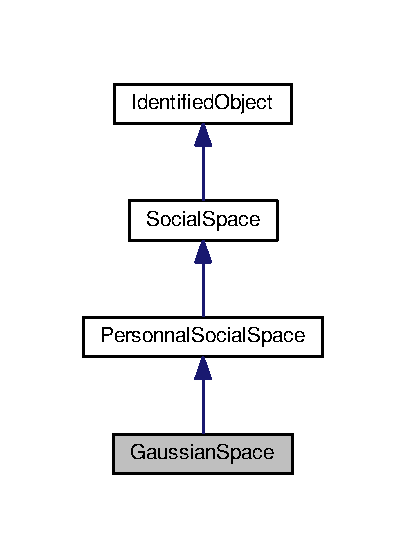
\includegraphics[width=195pt]{classGaussianSpace__inherit__graph}
\end{center}
\end{figure}


Collaboration diagram for Gaussian\+Space\+:\nopagebreak
\begin{figure}[H]
\begin{center}
\leavevmode
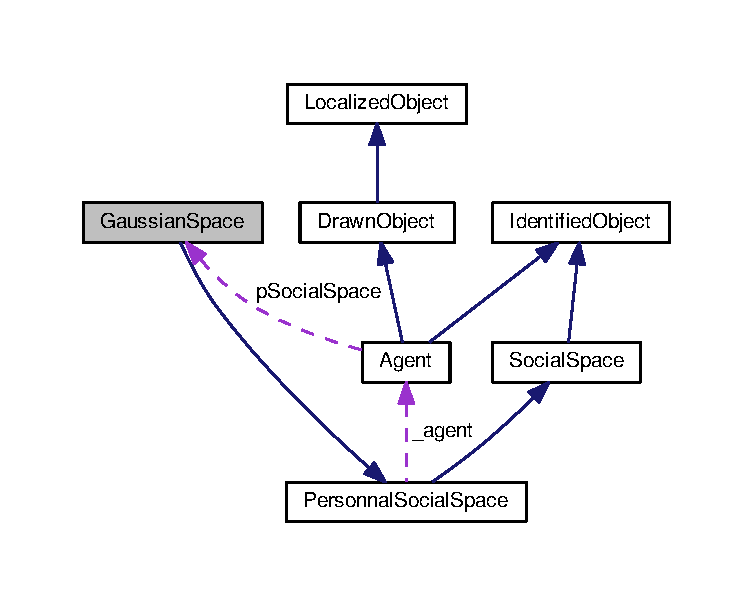
\includegraphics[width=350pt]{classGaussianSpace__coll__graph}
\end{center}
\end{figure}
\subsection*{Public Member Functions}
\begin{DoxyCompactItemize}
\item 
\hyperlink{classGaussianSpace_a04f0be340911fe421b6d226e7be936e1}{Gaussian\+Space} (\hyperlink{classAgent}{Agent} $\ast$agent, int \hyperlink{classIdentifiedObject_ad044a317a9b573a3d1bcd025df166eb5}{id}=0)
\begin{DoxyCompactList}\small\item\em Constructor. \end{DoxyCompactList}\item 
virtual \hyperlink{classGaussianSpace_aff1535add265d12148ba8eca0766e268}{$\sim$\+Gaussian\+Space} ()
\begin{DoxyCompactList}\small\item\em Destructor. \end{DoxyCompactList}\item 
double \hyperlink{classGaussianSpace_a8b1dec9d243861c80d63d3323a36f182}{phi} (Vector3d tested\+Real\+Point)
\begin{DoxyCompactList}\small\item\em Compute the value of the \hyperlink{classGaussianSpace}{Gaussian\+Space} at a given point in space. \end{DoxyCompactList}\end{DoxyCompactItemize}
\subsection*{Additional Inherited Members}


\subsection{Detailed Description}
This class is an implementation of the \hyperlink{classPersonnalSocialSpace}{Personnal\+Social\+Space}. 

This class is an implementation of the \hyperlink{classPersonnalSocialSpace}{Personnal\+Social\+Space} represented by a 2D gaussian mixture model model based on interpersonal distances. 

\subsection{Constructor \& Destructor Documentation}
\index{Gaussian\+Space@{Gaussian\+Space}!Gaussian\+Space@{Gaussian\+Space}}
\index{Gaussian\+Space@{Gaussian\+Space}!Gaussian\+Space@{Gaussian\+Space}}
\subsubsection[{\texorpdfstring{Gaussian\+Space(\+Agent $\ast$agent, int id=0)}{GaussianSpace(Agent *agent, int id=0)}}]{\setlength{\rightskip}{0pt plus 5cm}Gaussian\+Space\+::\+Gaussian\+Space (
\begin{DoxyParamCaption}
\item[{{\bf Agent} $\ast$}]{agent, }
\item[{int}]{id = {\ttfamily 0}}
\end{DoxyParamCaption}
)}\hypertarget{classGaussianSpace_a04f0be340911fe421b6d226e7be936e1}{}\label{classGaussianSpace_a04f0be340911fe421b6d226e7be936e1}


Constructor. 

Constructor of the \hyperlink{classGaussianSpace}{Gaussian\+Space} class


\begin{DoxyParams}{Parameters}
{\em agent} & \+: The \hyperlink{classAgent}{Agent} related to the \hyperlink{classGaussianSpace}{Gaussian\+Space} \\
\hline
{\em id} & \+: The unique identifier of the \hyperlink{classGaussianSpace}{Gaussian\+Space} \\
\hline
\end{DoxyParams}
\index{Gaussian\+Space@{Gaussian\+Space}!````~Gaussian\+Space@{$\sim$\+Gaussian\+Space}}
\index{````~Gaussian\+Space@{$\sim$\+Gaussian\+Space}!Gaussian\+Space@{Gaussian\+Space}}
\subsubsection[{\texorpdfstring{$\sim$\+Gaussian\+Space()}{~GaussianSpace()}}]{\setlength{\rightskip}{0pt plus 5cm}Gaussian\+Space\+::$\sim$\+Gaussian\+Space (
\begin{DoxyParamCaption}
{}
\end{DoxyParamCaption}
)\hspace{0.3cm}{\ttfamily [virtual]}}\hypertarget{classGaussianSpace_aff1535add265d12148ba8eca0766e268}{}\label{classGaussianSpace_aff1535add265d12148ba8eca0766e268}


Destructor. 

Destructor of the \hyperlink{classGaussianSpace}{Gaussian\+Space} class 

\subsection{Member Function Documentation}
\index{Gaussian\+Space@{Gaussian\+Space}!phi@{phi}}
\index{phi@{phi}!Gaussian\+Space@{Gaussian\+Space}}
\subsubsection[{\texorpdfstring{phi(\+Vector3d tested\+Real\+Point)}{phi(Vector3d testedRealPoint)}}]{\setlength{\rightskip}{0pt plus 5cm}double Gaussian\+Space\+::phi (
\begin{DoxyParamCaption}
\item[{Vector3d}]{tested\+Real\+Point}
\end{DoxyParamCaption}
)}\hypertarget{classGaussianSpace_a8b1dec9d243861c80d63d3323a36f182}{}\label{classGaussianSpace_a8b1dec9d243861c80d63d3323a36f182}


Compute the value of the \hyperlink{classGaussianSpace}{Gaussian\+Space} at a given point in space. 


\begin{DoxyParams}{Parameters}
{\em tested\+Real\+Point} & \+: The coordinates of the point in the real frame coordinates \hyperlink{classWorld}{World}\\
\hline
\end{DoxyParams}
\begin{DoxyReturn}{Returns}
The value of the \hyperlink{classGaussianSpace}{Gaussian\+Space} at the given point 
\end{DoxyReturn}


The documentation for this class was generated from the following files\+:\begin{DoxyCompactItemize}
\item 
src/social\+Space/\hyperlink{GaussianSpace_8h}{Gaussian\+Space.\+h}\item 
src/social\+Space/\hyperlink{GaussianSpace_8cpp}{Gaussian\+Space.\+cpp}\end{DoxyCompactItemize}

\hypertarget{classGridCell}{}\section{Grid\+Cell Class Reference}
\label{classGridCell}\index{Grid\+Cell@{Grid\+Cell}}


This class represent a cell in the \hyperlink{classGridMap}{Grid\+Map}.  




{\ttfamily \#include $<$Grid\+Cell.\+h$>$}



Inheritance diagram for Grid\+Cell\+:\nopagebreak
\begin{figure}[H]
\begin{center}
\leavevmode
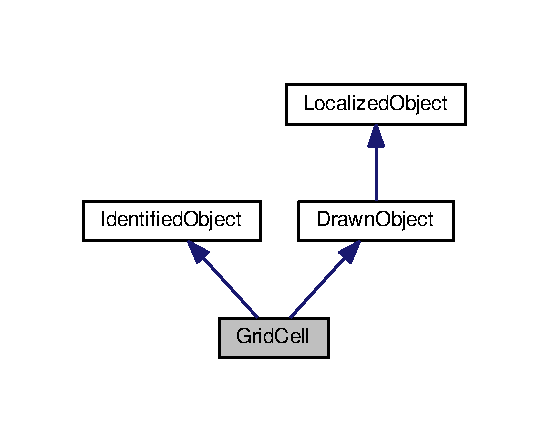
\includegraphics[width=264pt]{classGridCell__inherit__graph}
\end{center}
\end{figure}


Collaboration diagram for Grid\+Cell\+:\nopagebreak
\begin{figure}[H]
\begin{center}
\leavevmode
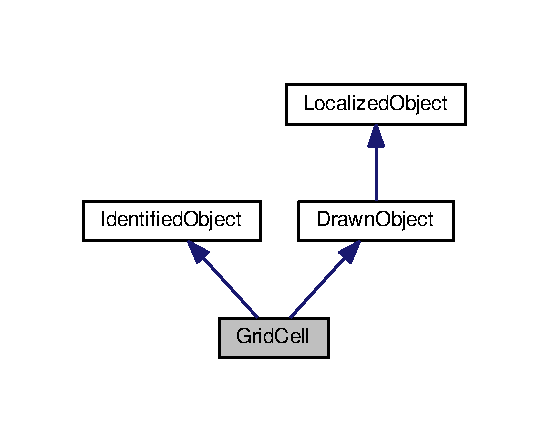
\includegraphics[width=264pt]{classGridCell__coll__graph}
\end{center}
\end{figure}
\subsection*{Public Member Functions}
\begin{DoxyCompactItemize}
\item 
\hyperlink{classGridCell_aefc88a474d5b3e60c3c5ae919c7e1bf9}{Grid\+Cell} (double size, double value=0, Vector3d \hyperlink{classLocalizedObject_a340834deefc9e5c39da1f26c4ebf4f8c}{position}=Vector3d(), int \hyperlink{classIdentifiedObject_ad044a317a9b573a3d1bcd025df166eb5}{id}=0)
\begin{DoxyCompactList}\small\item\em Constructor. \end{DoxyCompactList}\item 
virtual \hyperlink{classGridCell_a8952d31ed1dd16eb5fb32fff9be95c7c}{$\sim$\+Grid\+Cell} ()
\begin{DoxyCompactList}\small\item\em Destructor. \end{DoxyCompactList}\item 
double \hyperlink{classGridCell_a04f6b968f8a878747f196c582288f2e9}{get\+Value} () const 
\begin{DoxyCompactList}\small\item\em Simple getter. \end{DoxyCompactList}\item 
void \hyperlink{classGridCell_a450cb7b243e81d70583f24ae0902568d}{set\+Value} (double value)
\begin{DoxyCompactList}\small\item\em Simple setter. \end{DoxyCompactList}\item 
double \hyperlink{classGridCell_a4d2ec9a305c1e5a3508420f2b75e0721}{get\+Size} () const 
\begin{DoxyCompactList}\small\item\em Simple getter. \end{DoxyCompactList}\item 
void \hyperlink{classGridCell_a10b03ef94c1fbc4145692c846c14809c}{set\+Size} (double size)
\begin{DoxyCompactList}\small\item\em Simple setter. \end{DoxyCompactList}\item 
bool \hyperlink{classGridCell_acc9dad8cc0fbf272a4df442329cfff89}{is\+Border\+Enabled} () const 
\begin{DoxyCompactList}\small\item\em Simple getter. \end{DoxyCompactList}\item 
void \hyperlink{classGridCell_a11419a8819e3352575dccb4a860626e0}{set\+Border\+Enabled} (bool \hyperlink{classGridCell_aa153cae8dd39f3435f0d94af62fc506c}{border\+Enabled}=true)
\begin{DoxyCompactList}\small\item\em Simple setter. \end{DoxyCompactList}\item 
double \hyperlink{classGridCell_a5ca76c4f5366e038bb04d69ebba1bfaa}{get\+A\+Star\+Score} () const 
\begin{DoxyCompactList}\small\item\em Simple getter. \end{DoxyCompactList}\item 
void \hyperlink{classGridCell_aba04e37a148ccdf854fa3d1212ae53e8}{set\+A\+Star\+Score} (int star\+Score)
\begin{DoxyCompactList}\small\item\em Simple setter. \end{DoxyCompactList}\item 
bool \hyperlink{classGridCell_abb1ed437dca40c20cf9d7ea8a46841bd}{is\+Cell\+Selected} () const 
\begin{DoxyCompactList}\small\item\em Simple getter. \end{DoxyCompactList}\item 
void \hyperlink{classGridCell_ae122cd7653166197f3956b26416f2e0a}{set\+Cell\+Selected} (bool \hyperlink{classGridCell_ace80d646d21ff2134df71a64a4b4222d}{cell\+Selected}=true)
\begin{DoxyCompactList}\small\item\em Simple setter. \end{DoxyCompactList}\item 
bool \hyperlink{classGridCell_af0d7942180a406779e395179a7882c6d}{is\+Frontier} () const 
\begin{DoxyCompactList}\small\item\em Simple getter. \end{DoxyCompactList}\item 
void \hyperlink{classGridCell_a59db9ea256eeb5f9a2ec6130794c7dcc}{set\+Frontier} (bool \hyperlink{classGridCell_ab8c610dccff54254896b67d34cb36b35}{frontier}=true)
\begin{DoxyCompactList}\small\item\em Simple setter. \end{DoxyCompactList}\item 
bool \hyperlink{classGridCell_a071e0d4c217d7992ed31cdcba1c1c10d}{is\+Processed} () const 
\begin{DoxyCompactList}\small\item\em Simple getter. \end{DoxyCompactList}\item 
void \hyperlink{classGridCell_a72581a1a587bebaba02fb36d419d3768}{set\+Processed} (bool \hyperlink{classGridCell_acd279e15b141714d74586ba0a05e9d7b}{processed}=true)
\begin{DoxyCompactList}\small\item\em Simple setter. \end{DoxyCompactList}\item 
bool \hyperlink{classGridCell_a556d638eef4f4135158dcdcff87f761a}{is\+Goal} () const 
\begin{DoxyCompactList}\small\item\em Simple getter. \end{DoxyCompactList}\item 
void \hyperlink{classGridCell_aa9092a59955a34313dea633eab05d4c8}{set\+Goal} (bool \hyperlink{classGridCell_afe1b6d3afa06397f1732c07cfd9111ed}{goal}=true)
\begin{DoxyCompactList}\small\item\em Simple setter. \end{DoxyCompactList}\item 
bool \hyperlink{classGridCell_a233cabce55d024827a351a91292f3b19}{is\+Start} () const 
\begin{DoxyCompactList}\small\item\em Simple getter. \end{DoxyCompactList}\item 
void \hyperlink{classGridCell_ad104aba9157bb24a30a6e802950ffd37}{set\+Start} (bool \hyperlink{classGridCell_ac9fb7e6a84df215d9a3888428fe63425}{start}=true)
\begin{DoxyCompactList}\small\item\em Simple setter. \end{DoxyCompactList}\item 
bool \hyperlink{classGridCell_a1adf0636dabff7aca3d815ac7f888607}{is\+Info\+Enabled} () const 
\begin{DoxyCompactList}\small\item\em Simple getter. \end{DoxyCompactList}\item 
void \hyperlink{classGridCell_ab6312c017289556a74736f4dcf3d0062}{set\+Info\+Enabled} (bool \hyperlink{classGridCell_a2dbb35023dd7a201c1c02569204cfd2e}{info\+Enabled}=true)
\begin{DoxyCompactList}\small\item\em Simple setter. \end{DoxyCompactList}\end{DoxyCompactItemize}
\subsection*{Protected Attributes}
\begin{DoxyCompactItemize}
\item 
double \hyperlink{classGridCell_a6da426a6abc1a134c69f1b81647d9cfa}{\+\_\+size}\hypertarget{classGridCell_a6da426a6abc1a134c69f1b81647d9cfa}{}\label{classGridCell_a6da426a6abc1a134c69f1b81647d9cfa}

\begin{DoxyCompactList}\small\item\em The size of the \hyperlink{classGridCell}{Grid\+Cell}. \end{DoxyCompactList}\item 
double \hyperlink{classGridCell_a933654fb91fed011c81b0a70af3e1f5a}{\+\_\+value}\hypertarget{classGridCell_a933654fb91fed011c81b0a70af3e1f5a}{}\label{classGridCell_a933654fb91fed011c81b0a70af3e1f5a}

\begin{DoxyCompactList}\small\item\em The value of the \hyperlink{classGridCell}{Grid\+Cell}. \end{DoxyCompactList}\item 
bool \hyperlink{classGridCell_aa153cae8dd39f3435f0d94af62fc506c}{border\+Enabled} = false\hypertarget{classGridCell_aa153cae8dd39f3435f0d94af62fc506c}{}\label{classGridCell_aa153cae8dd39f3435f0d94af62fc506c}

\begin{DoxyCompactList}\small\item\em Enable of disable \hyperlink{classGridCell}{Grid\+Cell} border drawing. \end{DoxyCompactList}\item 
double \hyperlink{classGridCell_a2c12f31b0b0f64b0c90624ab596cd0e6}{\+\_\+a\+Star\+Score} = -\/1\hypertarget{classGridCell_a2c12f31b0b0f64b0c90624ab596cd0e6}{}\label{classGridCell_a2c12f31b0b0f64b0c90624ab596cd0e6}

\begin{DoxyCompactList}\small\item\em The A$\ast$ score of the \hyperlink{classGridCell}{Grid\+Cell}. \end{DoxyCompactList}\item 
bool \hyperlink{classGridCell_ace80d646d21ff2134df71a64a4b4222d}{cell\+Selected} = false\hypertarget{classGridCell_ace80d646d21ff2134df71a64a4b4222d}{}\label{classGridCell_ace80d646d21ff2134df71a64a4b4222d}

\begin{DoxyCompactList}\small\item\em Select of deselect \hyperlink{classGridCell}{Grid\+Cell} (change drawing color) \end{DoxyCompactList}\item 
bool \hyperlink{classGridCell_ab8c610dccff54254896b67d34cb36b35}{frontier} = false\hypertarget{classGridCell_ab8c610dccff54254896b67d34cb36b35}{}\label{classGridCell_ab8c610dccff54254896b67d34cb36b35}

\begin{DoxyCompactList}\small\item\em If the \hyperlink{classGridCell}{Grid\+Cell} is a frontier (change drawing color) \end{DoxyCompactList}\item 
bool \hyperlink{classGridCell_acd279e15b141714d74586ba0a05e9d7b}{processed} = false\hypertarget{classGridCell_acd279e15b141714d74586ba0a05e9d7b}{}\label{classGridCell_acd279e15b141714d74586ba0a05e9d7b}

\begin{DoxyCompactList}\small\item\em If the \hyperlink{classGridCell}{Grid\+Cell} has been processed (change drawing color) \end{DoxyCompactList}\item 
bool \hyperlink{classGridCell_afe1b6d3afa06397f1732c07cfd9111ed}{goal} = false\hypertarget{classGridCell_afe1b6d3afa06397f1732c07cfd9111ed}{}\label{classGridCell_afe1b6d3afa06397f1732c07cfd9111ed}

\begin{DoxyCompactList}\small\item\em If the \hyperlink{classGridCell}{Grid\+Cell} is the goal to reach (change drawing color) \end{DoxyCompactList}\item 
bool \hyperlink{classGridCell_ac9fb7e6a84df215d9a3888428fe63425}{start} = false\hypertarget{classGridCell_ac9fb7e6a84df215d9a3888428fe63425}{}\label{classGridCell_ac9fb7e6a84df215d9a3888428fe63425}

\begin{DoxyCompactList}\small\item\em If the \hyperlink{classGridCell}{Grid\+Cell} is the starting point (change drawing color) \end{DoxyCompactList}\item 
bool \hyperlink{classGridCell_a2dbb35023dd7a201c1c02569204cfd2e}{info\+Enabled} = false\hypertarget{classGridCell_a2dbb35023dd7a201c1c02569204cfd2e}{}\label{classGridCell_a2dbb35023dd7a201c1c02569204cfd2e}

\begin{DoxyCompactList}\small\item\em Enable of disable \hyperlink{classGridCell}{Grid\+Cell} informations drawing. \end{DoxyCompactList}\end{DoxyCompactItemize}


\subsection{Detailed Description}
This class represent a cell in the \hyperlink{classGridMap}{Grid\+Map}. 

\subsection{Constructor \& Destructor Documentation}
\index{Grid\+Cell@{Grid\+Cell}!Grid\+Cell@{Grid\+Cell}}
\index{Grid\+Cell@{Grid\+Cell}!Grid\+Cell@{Grid\+Cell}}
\subsubsection[{\texorpdfstring{Grid\+Cell(double size, double value=0, Vector3d position=\+Vector3d(), int id=0)}{GridCell(double size, double value=0, Vector3d position=Vector3d(), int id=0)}}]{\setlength{\rightskip}{0pt plus 5cm}Grid\+Cell\+::\+Grid\+Cell (
\begin{DoxyParamCaption}
\item[{double}]{size, }
\item[{double}]{value = {\ttfamily 0}, }
\item[{Vector3d}]{position = {\ttfamily Vector3d()}, }
\item[{int}]{id = {\ttfamily 0}}
\end{DoxyParamCaption}
)}\hypertarget{classGridCell_aefc88a474d5b3e60c3c5ae919c7e1bf9}{}\label{classGridCell_aefc88a474d5b3e60c3c5ae919c7e1bf9}


Constructor. 

Constructor of the \hyperlink{classGridCell}{Grid\+Cell} class


\begin{DoxyParams}{Parameters}
{\em size} & \+: The size of the \hyperlink{classGridCell}{Grid\+Cell} \\
\hline
{\em value} & \+: The initial value of the \hyperlink{classGridCell}{Grid\+Cell} \\
\hline
{\em position} & \+: The position of the \hyperlink{classGridCell}{Grid\+Cell} in real coordinate \\
\hline
{\em id} & \+: The unique identifier of the \hyperlink{classGridCell}{Grid\+Cell} \\
\hline
\end{DoxyParams}
\index{Grid\+Cell@{Grid\+Cell}!````~Grid\+Cell@{$\sim$\+Grid\+Cell}}
\index{````~Grid\+Cell@{$\sim$\+Grid\+Cell}!Grid\+Cell@{Grid\+Cell}}
\subsubsection[{\texorpdfstring{$\sim$\+Grid\+Cell()}{~GridCell()}}]{\setlength{\rightskip}{0pt plus 5cm}Grid\+Cell\+::$\sim$\+Grid\+Cell (
\begin{DoxyParamCaption}
{}
\end{DoxyParamCaption}
)\hspace{0.3cm}{\ttfamily [virtual]}}\hypertarget{classGridCell_a8952d31ed1dd16eb5fb32fff9be95c7c}{}\label{classGridCell_a8952d31ed1dd16eb5fb32fff9be95c7c}


Destructor. 

Destructor of the \hyperlink{classGridCell}{Grid\+Cell} class 

\subsection{Member Function Documentation}
\index{Grid\+Cell@{Grid\+Cell}!get\+A\+Star\+Score@{get\+A\+Star\+Score}}
\index{get\+A\+Star\+Score@{get\+A\+Star\+Score}!Grid\+Cell@{Grid\+Cell}}
\subsubsection[{\texorpdfstring{get\+A\+Star\+Score() const }{getAStarScore() const }}]{\setlength{\rightskip}{0pt plus 5cm}double Grid\+Cell\+::get\+A\+Star\+Score (
\begin{DoxyParamCaption}
{}
\end{DoxyParamCaption}
) const}\hypertarget{classGridCell_a5ca76c4f5366e038bb04d69ebba1bfaa}{}\label{classGridCell_a5ca76c4f5366e038bb04d69ebba1bfaa}


Simple getter. 

\begin{DoxyReturn}{Returns}
a\+Star\+Score 
\end{DoxyReturn}
\index{Grid\+Cell@{Grid\+Cell}!get\+Size@{get\+Size}}
\index{get\+Size@{get\+Size}!Grid\+Cell@{Grid\+Cell}}
\subsubsection[{\texorpdfstring{get\+Size() const }{getSize() const }}]{\setlength{\rightskip}{0pt plus 5cm}double Grid\+Cell\+::get\+Size (
\begin{DoxyParamCaption}
{}
\end{DoxyParamCaption}
) const}\hypertarget{classGridCell_a4d2ec9a305c1e5a3508420f2b75e0721}{}\label{classGridCell_a4d2ec9a305c1e5a3508420f2b75e0721}


Simple getter. 

\begin{DoxyReturn}{Returns}
size 
\end{DoxyReturn}
\index{Grid\+Cell@{Grid\+Cell}!get\+Value@{get\+Value}}
\index{get\+Value@{get\+Value}!Grid\+Cell@{Grid\+Cell}}
\subsubsection[{\texorpdfstring{get\+Value() const }{getValue() const }}]{\setlength{\rightskip}{0pt plus 5cm}double Grid\+Cell\+::get\+Value (
\begin{DoxyParamCaption}
{}
\end{DoxyParamCaption}
) const}\hypertarget{classGridCell_a04f6b968f8a878747f196c582288f2e9}{}\label{classGridCell_a04f6b968f8a878747f196c582288f2e9}


Simple getter. 

\begin{DoxyReturn}{Returns}
value 
\end{DoxyReturn}
\index{Grid\+Cell@{Grid\+Cell}!is\+Border\+Enabled@{is\+Border\+Enabled}}
\index{is\+Border\+Enabled@{is\+Border\+Enabled}!Grid\+Cell@{Grid\+Cell}}
\subsubsection[{\texorpdfstring{is\+Border\+Enabled() const }{isBorderEnabled() const }}]{\setlength{\rightskip}{0pt plus 5cm}bool Grid\+Cell\+::is\+Border\+Enabled (
\begin{DoxyParamCaption}
{}
\end{DoxyParamCaption}
) const}\hypertarget{classGridCell_acc9dad8cc0fbf272a4df442329cfff89}{}\label{classGridCell_acc9dad8cc0fbf272a4df442329cfff89}


Simple getter. 

\begin{DoxyReturn}{Returns}
border\+Enabled 
\end{DoxyReturn}
\index{Grid\+Cell@{Grid\+Cell}!is\+Cell\+Selected@{is\+Cell\+Selected}}
\index{is\+Cell\+Selected@{is\+Cell\+Selected}!Grid\+Cell@{Grid\+Cell}}
\subsubsection[{\texorpdfstring{is\+Cell\+Selected() const }{isCellSelected() const }}]{\setlength{\rightskip}{0pt plus 5cm}bool Grid\+Cell\+::is\+Cell\+Selected (
\begin{DoxyParamCaption}
{}
\end{DoxyParamCaption}
) const}\hypertarget{classGridCell_abb1ed437dca40c20cf9d7ea8a46841bd}{}\label{classGridCell_abb1ed437dca40c20cf9d7ea8a46841bd}


Simple getter. 

\begin{DoxyReturn}{Returns}
cell\+Selected 
\end{DoxyReturn}
\index{Grid\+Cell@{Grid\+Cell}!is\+Frontier@{is\+Frontier}}
\index{is\+Frontier@{is\+Frontier}!Grid\+Cell@{Grid\+Cell}}
\subsubsection[{\texorpdfstring{is\+Frontier() const }{isFrontier() const }}]{\setlength{\rightskip}{0pt plus 5cm}bool Grid\+Cell\+::is\+Frontier (
\begin{DoxyParamCaption}
{}
\end{DoxyParamCaption}
) const}\hypertarget{classGridCell_af0d7942180a406779e395179a7882c6d}{}\label{classGridCell_af0d7942180a406779e395179a7882c6d}


Simple getter. 

\begin{DoxyReturn}{Returns}
frontier 
\end{DoxyReturn}
\index{Grid\+Cell@{Grid\+Cell}!is\+Goal@{is\+Goal}}
\index{is\+Goal@{is\+Goal}!Grid\+Cell@{Grid\+Cell}}
\subsubsection[{\texorpdfstring{is\+Goal() const }{isGoal() const }}]{\setlength{\rightskip}{0pt plus 5cm}bool Grid\+Cell\+::is\+Goal (
\begin{DoxyParamCaption}
{}
\end{DoxyParamCaption}
) const}\hypertarget{classGridCell_a556d638eef4f4135158dcdcff87f761a}{}\label{classGridCell_a556d638eef4f4135158dcdcff87f761a}


Simple getter. 

\begin{DoxyReturn}{Returns}
goal 
\end{DoxyReturn}
\index{Grid\+Cell@{Grid\+Cell}!is\+Info\+Enabled@{is\+Info\+Enabled}}
\index{is\+Info\+Enabled@{is\+Info\+Enabled}!Grid\+Cell@{Grid\+Cell}}
\subsubsection[{\texorpdfstring{is\+Info\+Enabled() const }{isInfoEnabled() const }}]{\setlength{\rightskip}{0pt plus 5cm}bool Grid\+Cell\+::is\+Info\+Enabled (
\begin{DoxyParamCaption}
{}
\end{DoxyParamCaption}
) const}\hypertarget{classGridCell_a1adf0636dabff7aca3d815ac7f888607}{}\label{classGridCell_a1adf0636dabff7aca3d815ac7f888607}


Simple getter. 

\begin{DoxyReturn}{Returns}
info\+Enabled 
\end{DoxyReturn}
\index{Grid\+Cell@{Grid\+Cell}!is\+Processed@{is\+Processed}}
\index{is\+Processed@{is\+Processed}!Grid\+Cell@{Grid\+Cell}}
\subsubsection[{\texorpdfstring{is\+Processed() const }{isProcessed() const }}]{\setlength{\rightskip}{0pt plus 5cm}bool Grid\+Cell\+::is\+Processed (
\begin{DoxyParamCaption}
{}
\end{DoxyParamCaption}
) const}\hypertarget{classGridCell_a071e0d4c217d7992ed31cdcba1c1c10d}{}\label{classGridCell_a071e0d4c217d7992ed31cdcba1c1c10d}


Simple getter. 

\begin{DoxyReturn}{Returns}
processed 
\end{DoxyReturn}
\index{Grid\+Cell@{Grid\+Cell}!is\+Start@{is\+Start}}
\index{is\+Start@{is\+Start}!Grid\+Cell@{Grid\+Cell}}
\subsubsection[{\texorpdfstring{is\+Start() const }{isStart() const }}]{\setlength{\rightskip}{0pt plus 5cm}bool Grid\+Cell\+::is\+Start (
\begin{DoxyParamCaption}
{}
\end{DoxyParamCaption}
) const}\hypertarget{classGridCell_a233cabce55d024827a351a91292f3b19}{}\label{classGridCell_a233cabce55d024827a351a91292f3b19}


Simple getter. 

\begin{DoxyReturn}{Returns}
start 
\end{DoxyReturn}
\index{Grid\+Cell@{Grid\+Cell}!set\+A\+Star\+Score@{set\+A\+Star\+Score}}
\index{set\+A\+Star\+Score@{set\+A\+Star\+Score}!Grid\+Cell@{Grid\+Cell}}
\subsubsection[{\texorpdfstring{set\+A\+Star\+Score(int star\+Score)}{setAStarScore(int starScore)}}]{\setlength{\rightskip}{0pt plus 5cm}void Grid\+Cell\+::set\+A\+Star\+Score (
\begin{DoxyParamCaption}
\item[{int}]{star\+Score}
\end{DoxyParamCaption}
)}\hypertarget{classGridCell_aba04e37a148ccdf854fa3d1212ae53e8}{}\label{classGridCell_aba04e37a148ccdf854fa3d1212ae53e8}


Simple setter. 


\begin{DoxyParams}{Parameters}
{\em star\+Score} & \\
\hline
\end{DoxyParams}
\index{Grid\+Cell@{Grid\+Cell}!set\+Border\+Enabled@{set\+Border\+Enabled}}
\index{set\+Border\+Enabled@{set\+Border\+Enabled}!Grid\+Cell@{Grid\+Cell}}
\subsubsection[{\texorpdfstring{set\+Border\+Enabled(bool border\+Enabled=true)}{setBorderEnabled(bool borderEnabled=true)}}]{\setlength{\rightskip}{0pt plus 5cm}void Grid\+Cell\+::set\+Border\+Enabled (
\begin{DoxyParamCaption}
\item[{bool}]{border\+Enabled = {\ttfamily true}}
\end{DoxyParamCaption}
)}\hypertarget{classGridCell_a11419a8819e3352575dccb4a860626e0}{}\label{classGridCell_a11419a8819e3352575dccb4a860626e0}


Simple setter. 


\begin{DoxyParams}{Parameters}
{\em border\+Enabled} & \\
\hline
\end{DoxyParams}
\index{Grid\+Cell@{Grid\+Cell}!set\+Cell\+Selected@{set\+Cell\+Selected}}
\index{set\+Cell\+Selected@{set\+Cell\+Selected}!Grid\+Cell@{Grid\+Cell}}
\subsubsection[{\texorpdfstring{set\+Cell\+Selected(bool cell\+Selected=true)}{setCellSelected(bool cellSelected=true)}}]{\setlength{\rightskip}{0pt plus 5cm}void Grid\+Cell\+::set\+Cell\+Selected (
\begin{DoxyParamCaption}
\item[{bool}]{cell\+Selected = {\ttfamily true}}
\end{DoxyParamCaption}
)}\hypertarget{classGridCell_ae122cd7653166197f3956b26416f2e0a}{}\label{classGridCell_ae122cd7653166197f3956b26416f2e0a}


Simple setter. 


\begin{DoxyParams}{Parameters}
{\em cell\+Selected} & \\
\hline
\end{DoxyParams}
\index{Grid\+Cell@{Grid\+Cell}!set\+Frontier@{set\+Frontier}}
\index{set\+Frontier@{set\+Frontier}!Grid\+Cell@{Grid\+Cell}}
\subsubsection[{\texorpdfstring{set\+Frontier(bool frontier=true)}{setFrontier(bool frontier=true)}}]{\setlength{\rightskip}{0pt plus 5cm}void Grid\+Cell\+::set\+Frontier (
\begin{DoxyParamCaption}
\item[{bool}]{frontier = {\ttfamily true}}
\end{DoxyParamCaption}
)}\hypertarget{classGridCell_a59db9ea256eeb5f9a2ec6130794c7dcc}{}\label{classGridCell_a59db9ea256eeb5f9a2ec6130794c7dcc}


Simple setter. 


\begin{DoxyParams}{Parameters}
{\em frontier} & \\
\hline
\end{DoxyParams}
\index{Grid\+Cell@{Grid\+Cell}!set\+Goal@{set\+Goal}}
\index{set\+Goal@{set\+Goal}!Grid\+Cell@{Grid\+Cell}}
\subsubsection[{\texorpdfstring{set\+Goal(bool goal=true)}{setGoal(bool goal=true)}}]{\setlength{\rightskip}{0pt plus 5cm}void Grid\+Cell\+::set\+Goal (
\begin{DoxyParamCaption}
\item[{bool}]{goal = {\ttfamily true}}
\end{DoxyParamCaption}
)}\hypertarget{classGridCell_aa9092a59955a34313dea633eab05d4c8}{}\label{classGridCell_aa9092a59955a34313dea633eab05d4c8}


Simple setter. 


\begin{DoxyParams}{Parameters}
{\em goal} & \\
\hline
\end{DoxyParams}
\index{Grid\+Cell@{Grid\+Cell}!set\+Info\+Enabled@{set\+Info\+Enabled}}
\index{set\+Info\+Enabled@{set\+Info\+Enabled}!Grid\+Cell@{Grid\+Cell}}
\subsubsection[{\texorpdfstring{set\+Info\+Enabled(bool info\+Enabled=true)}{setInfoEnabled(bool infoEnabled=true)}}]{\setlength{\rightskip}{0pt plus 5cm}void Grid\+Cell\+::set\+Info\+Enabled (
\begin{DoxyParamCaption}
\item[{bool}]{info\+Enabled = {\ttfamily true}}
\end{DoxyParamCaption}
)}\hypertarget{classGridCell_ab6312c017289556a74736f4dcf3d0062}{}\label{classGridCell_ab6312c017289556a74736f4dcf3d0062}


Simple setter. 


\begin{DoxyParams}{Parameters}
{\em info\+Enabled} & \\
\hline
\end{DoxyParams}
\index{Grid\+Cell@{Grid\+Cell}!set\+Processed@{set\+Processed}}
\index{set\+Processed@{set\+Processed}!Grid\+Cell@{Grid\+Cell}}
\subsubsection[{\texorpdfstring{set\+Processed(bool processed=true)}{setProcessed(bool processed=true)}}]{\setlength{\rightskip}{0pt plus 5cm}void Grid\+Cell\+::set\+Processed (
\begin{DoxyParamCaption}
\item[{bool}]{processed = {\ttfamily true}}
\end{DoxyParamCaption}
)}\hypertarget{classGridCell_a72581a1a587bebaba02fb36d419d3768}{}\label{classGridCell_a72581a1a587bebaba02fb36d419d3768}


Simple setter. 


\begin{DoxyParams}{Parameters}
{\em processed} & \\
\hline
\end{DoxyParams}
\index{Grid\+Cell@{Grid\+Cell}!set\+Size@{set\+Size}}
\index{set\+Size@{set\+Size}!Grid\+Cell@{Grid\+Cell}}
\subsubsection[{\texorpdfstring{set\+Size(double size)}{setSize(double size)}}]{\setlength{\rightskip}{0pt plus 5cm}void Grid\+Cell\+::set\+Size (
\begin{DoxyParamCaption}
\item[{double}]{size}
\end{DoxyParamCaption}
)}\hypertarget{classGridCell_a10b03ef94c1fbc4145692c846c14809c}{}\label{classGridCell_a10b03ef94c1fbc4145692c846c14809c}


Simple setter. 


\begin{DoxyParams}{Parameters}
{\em size} & \\
\hline
\end{DoxyParams}
\index{Grid\+Cell@{Grid\+Cell}!set\+Start@{set\+Start}}
\index{set\+Start@{set\+Start}!Grid\+Cell@{Grid\+Cell}}
\subsubsection[{\texorpdfstring{set\+Start(bool start=true)}{setStart(bool start=true)}}]{\setlength{\rightskip}{0pt plus 5cm}void Grid\+Cell\+::set\+Start (
\begin{DoxyParamCaption}
\item[{bool}]{start = {\ttfamily true}}
\end{DoxyParamCaption}
)}\hypertarget{classGridCell_ad104aba9157bb24a30a6e802950ffd37}{}\label{classGridCell_ad104aba9157bb24a30a6e802950ffd37}


Simple setter. 


\begin{DoxyParams}{Parameters}
{\em start} & \\
\hline
\end{DoxyParams}
\index{Grid\+Cell@{Grid\+Cell}!set\+Value@{set\+Value}}
\index{set\+Value@{set\+Value}!Grid\+Cell@{Grid\+Cell}}
\subsubsection[{\texorpdfstring{set\+Value(double value)}{setValue(double value)}}]{\setlength{\rightskip}{0pt plus 5cm}void Grid\+Cell\+::set\+Value (
\begin{DoxyParamCaption}
\item[{double}]{value}
\end{DoxyParamCaption}
)}\hypertarget{classGridCell_a450cb7b243e81d70583f24ae0902568d}{}\label{classGridCell_a450cb7b243e81d70583f24ae0902568d}


Simple setter. 


\begin{DoxyParams}{Parameters}
{\em value} & \\
\hline
\end{DoxyParams}


The documentation for this class was generated from the following files\+:\begin{DoxyCompactItemize}
\item 
src/world\+Representation/\hyperlink{GridCell_8h}{Grid\+Cell.\+h}\item 
src/world\+Representation/\hyperlink{GridCell_8cpp}{Grid\+Cell.\+cpp}\end{DoxyCompactItemize}

\hypertarget{classGridMap}{}\section{Grid\+Map Class Reference}
\label{classGridMap}\index{Grid\+Map@{Grid\+Map}}


This class manage the 2D \hyperlink{classGridMap}{Grid\+Map} computed from the Agents \hyperlink{classSocialSpace}{Social\+Space}.  




{\ttfamily \#include $<$Grid\+Map.\+h$>$}



Inheritance diagram for Grid\+Map\+:\nopagebreak
\begin{figure}[H]
\begin{center}
\leavevmode
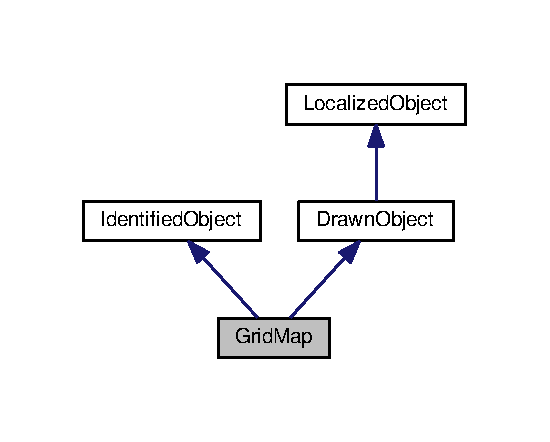
\includegraphics[width=264pt]{classGridMap__inherit__graph}
\end{center}
\end{figure}


Collaboration diagram for Grid\+Map\+:\nopagebreak
\begin{figure}[H]
\begin{center}
\leavevmode
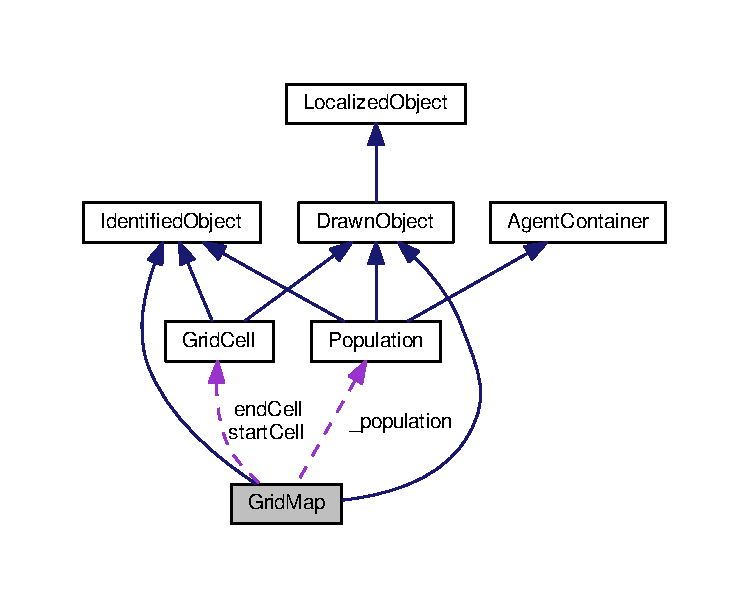
\includegraphics[width=350pt]{classGridMap__coll__graph}
\end{center}
\end{figure}
\subsection*{Classes}
\begin{DoxyCompactItemize}
\item 
struct \hyperlink{structGridMap_1_1CompaireVCell}{Compaire\+V\+Cell}
\begin{DoxyCompactList}\small\item\em Define an operator for \hyperlink{classGridCell}{Grid\+Cell} and associated g\+Score comparison for A$\ast$ algorithm. \end{DoxyCompactList}\end{DoxyCompactItemize}
\subsection*{Public Member Functions}
\begin{DoxyCompactItemize}
\item 
\hyperlink{classGridMap_aa5a60e82b2bf8b2005ef7c71e7080904}{Grid\+Map} (\hyperlink{classWorld}{World} $\ast$world, \hyperlink{classPopulation}{Population} $\ast$pop, double \hyperlink{classGridMap_a8481536f663251381674b71090754e1d}{resolution}=0.\+1)
\begin{DoxyCompactList}\small\item\em Constructor. \end{DoxyCompactList}\item 
virtual \hyperlink{classGridMap_a53cc0906130bae883f5d544480039118}{$\sim$\+Grid\+Map} ()
\begin{DoxyCompactList}\small\item\em Destructor. \end{DoxyCompactList}\item 
void \hyperlink{classGridMap_ac13f92dd7cdcfed701cf900eb592126b}{compute} ()\hypertarget{classGridMap_ac13f92dd7cdcfed701cf900eb592126b}{}\label{classGridMap_ac13f92dd7cdcfed701cf900eb592126b}

\begin{DoxyCompactList}\small\item\em Compute the value of each \hyperlink{classGridCell}{Grid\+Cell} in the \hyperlink{classGridMap}{Grid\+Map} based on Agents \hyperlink{classSocialSpace}{Social\+Space}. \end{DoxyCompactList}\item 
void \hyperlink{classGridMap_a5321e644c2398b2d0e50091b410f6ec3}{normalize} ()\hypertarget{classGridMap_a5321e644c2398b2d0e50091b410f6ec3}{}\label{classGridMap_a5321e644c2398b2d0e50091b410f6ec3}

\begin{DoxyCompactList}\small\item\em Normalize the Grid\+Cells value between 0 and 1. \end{DoxyCompactList}\item 
void \hyperlink{classGridMap_a5dcf97b44802b1ecf294f4e1fc79b94b}{update} ()\hypertarget{classGridMap_a5dcf97b44802b1ecf294f4e1fc79b94b}{}\label{classGridMap_a5dcf97b44802b1ecf294f4e1fc79b94b}

\begin{DoxyCompactList}\small\item\em Update the \hyperlink{classGridMap}{Grid\+Map} by calling compute and normalize function. \end{DoxyCompactList}\item 
void \hyperlink{classGridMap_a43a70209f5c8c5cf833500ce1d95880c}{deselect\+Cells} ()\hypertarget{classGridMap_a43a70209f5c8c5cf833500ce1d95880c}{}\label{classGridMap_a43a70209f5c8c5cf833500ce1d95880c}

\begin{DoxyCompactList}\small\item\em Set all \hyperlink{classGridCell}{Grid\+Cell} to selected False. \end{DoxyCompactList}\item 
int \hyperlink{classGridMap_a095c92e0c8abe909144cd9bf03fb2675}{path\+Finder\+Next\+Step} ()
\begin{DoxyCompactList}\small\item\em Compute one step of the A$\ast$ algorithm. \end{DoxyCompactList}\item 
void \hyperlink{classGridMap_ae2eb9ca9d4f2f1552f200ce4b9582d01}{reset\+Cell\+Color} ()\hypertarget{classGridMap_ae2eb9ca9d4f2f1552f200ce4b9582d01}{}\label{classGridMap_ae2eb9ca9d4f2f1552f200ce4b9582d01}

\begin{DoxyCompactList}\small\item\em Reset the color of all \hyperlink{classGridCell}{Grid\+Cell}. \end{DoxyCompactList}\item 
std\+::vector$<$ \hyperlink{classGridCell}{Grid\+Cell} $\ast$ $>$ \hyperlink{classGridMap_a9471e8e29679bb4e38f2a3011a394c4d}{construct\+Path} ()
\begin{DoxyCompactList}\small\item\em Build the path from A$\ast$ algorithm result. \end{DoxyCompactList}\item 
std\+::vector$<$ \hyperlink{classGridCell}{Grid\+Cell} $\ast$ $>$ \hyperlink{classGridMap_aecc6cb12f384e8049a4f029a68b11f73}{neighbors} (\hyperlink{classGridCell}{Grid\+Cell} $\ast$cell, bool allow\+Diagonal\+Move=true)
\begin{DoxyCompactList}\small\item\em Find the neighbors of a \hyperlink{classGridCell}{Grid\+Cell} in the \hyperlink{classGridMap}{Grid\+Map}. \end{DoxyCompactList}\item 
std\+::vector$<$ \hyperlink{classGridCell}{Grid\+Cell} $\ast$ $>$ \hyperlink{classGridMap_a976f63082aba927b21bc0d5a83c2261d}{find\+Path} (\hyperlink{classGridCell}{Grid\+Cell} $\ast$\hyperlink{classGridMap_a5c3e52ee3c6cc6183ac94d3cb31d6a93}{start\+Cell}, \hyperlink{classGridCell}{Grid\+Cell} $\ast$\hyperlink{classGridMap_a0ad10e901c423350fd0e578b256bb2f8}{end\+Cell})
\begin{DoxyCompactList}\small\item\em Find path between two given \hyperlink{classGridCell}{Grid\+Cell} in parameters. \end{DoxyCompactList}\item 
\hyperlink{classGridCell}{Grid\+Cell} $\ast$ \hyperlink{classGridMap_a2041007472f0be8fffe93cb1c25d8e9f}{get\+Cell} (unsigned int cell\+Id)
\begin{DoxyCompactList}\small\item\em Get a \hyperlink{classGridCell}{Grid\+Cell} in the \hyperlink{classGridMap}{Grid\+Map} by id. \end{DoxyCompactList}\item 
\hyperlink{classGridCell}{Grid\+Cell} $\ast$ \hyperlink{classGridMap_a5dd1d791747a4580e6c9d73a12b5953f}{get\+Cell} (double x, double y)
\begin{DoxyCompactList}\small\item\em find a \hyperlink{classGridCell}{Grid\+Cell} in the \hyperlink{classGridMap}{Grid\+Map} from its real coordinates \end{DoxyCompactList}\item 
void \hyperlink{classGridMap_a2c15016c5c2e1d2befdff013df12fe39}{set\+Info\+Enabled} (bool \hyperlink{classGridMap_ab106fa68828f14f788e697728b94992b}{info\+Enabled}=false)
\begin{DoxyCompactList}\small\item\em Simple setter. \end{DoxyCompactList}\item 
bool \hyperlink{classGridMap_a08ebd0d61670045ed7cbbdf33626d1af}{is\+Group\+Space\+Enabled} () const 
\begin{DoxyCompactList}\small\item\em Simple getter. \end{DoxyCompactList}\item 
void \hyperlink{classGridMap_a0923c16f8e6d2a08f02d8b32d0a5ef40}{set\+Group\+Space\+Enabled} (bool \hyperlink{classGridMap_ace7258ad25fea48c37b88e7de9c0b1b4}{group\+Space\+Enabled}=true)
\begin{DoxyCompactList}\small\item\em Simple setter. \end{DoxyCompactList}\item 
bool \hyperlink{classGridMap_ad37f0bb29e70f2cba3988fd1743d07d9}{is\+Personal\+Space\+Enabled} () const 
\begin{DoxyCompactList}\small\item\em Simple getter. \end{DoxyCompactList}\item 
void \hyperlink{classGridMap_ac5ed7378de3de7f4a4edddfb53a43af0}{set\+Personal\+Space\+Enabled} (bool \hyperlink{classGridMap_ab61a1f66414c31e4ffdd15cbd8c2f373}{personal\+Space\+Enabled}=true)
\begin{DoxyCompactList}\small\item\em Simple setter. \end{DoxyCompactList}\item 
bool \hyperlink{classGridMap_ab56b76831425dc0e3bf1c84d2a42bde1}{is\+Border\+Enabled} () const 
\begin{DoxyCompactList}\small\item\em Simple getter. \end{DoxyCompactList}\item 
void \hyperlink{classGridMap_a3ca0ec500c27b1c47ab0a73bceca44ea}{set\+Border\+Enabled} (bool \hyperlink{classGridMap_aad72652fe3a6ab78b47bce0c0daaaab5}{border\+Enabled}=true)
\begin{DoxyCompactList}\small\item\em Simple setter. \end{DoxyCompactList}\end{DoxyCompactItemize}
\subsection*{Protected Types}
\begin{DoxyCompactItemize}
\item 
typedef std\+::pair$<$ double, \hyperlink{classGridCell}{Grid\+Cell} $\ast$ $>$ \hyperlink{classGridMap_a3589e78d066f9c12b000f85f870afbc4}{V\+Cell}\hypertarget{classGridMap_a3589e78d066f9c12b000f85f870afbc4}{}\label{classGridMap_a3589e78d066f9c12b000f85f870afbc4}

\begin{DoxyCompactList}\small\item\em Define an operator for \hyperlink{classGridCell}{Grid\+Cell} and associated g\+Score comparison for A$\ast$ algorithm. \end{DoxyCompactList}\end{DoxyCompactItemize}
\subsection*{Protected Attributes}
\begin{DoxyCompactItemize}
\item 
\hyperlink{classPopulation}{Population} $\ast$ \hyperlink{classGridMap_ac43b2a50b73da8fe3c04635a6924dfc6}{\+\_\+population}\hypertarget{classGridMap_ac43b2a50b73da8fe3c04635a6924dfc6}{}\label{classGridMap_ac43b2a50b73da8fe3c04635a6924dfc6}

\begin{DoxyCompactList}\small\item\em The \hyperlink{classPopulation}{Population} related to the \hyperlink{classGridMap}{Grid\+Map}. \end{DoxyCompactList}\item 
double \hyperlink{classGridMap_a919ed90a283eb5ae30704e50e589a48f}{width}\hypertarget{classGridMap_a919ed90a283eb5ae30704e50e589a48f}{}\label{classGridMap_a919ed90a283eb5ae30704e50e589a48f}

\begin{DoxyCompactList}\small\item\em The real width of the \hyperlink{classGridMap}{Grid\+Map} in meter. \end{DoxyCompactList}\item 
double \hyperlink{classGridMap_a19dc2d36c3064698b34ef59433378b1a}{height}\hypertarget{classGridMap_a19dc2d36c3064698b34ef59433378b1a}{}\label{classGridMap_a19dc2d36c3064698b34ef59433378b1a}

\begin{DoxyCompactList}\small\item\em The real height of the \hyperlink{classGridMap}{Grid\+Map} in meter. \end{DoxyCompactList}\item 
double \hyperlink{classGridMap_a8481536f663251381674b71090754e1d}{resolution}\hypertarget{classGridMap_a8481536f663251381674b71090754e1d}{}\label{classGridMap_a8481536f663251381674b71090754e1d}

\begin{DoxyCompactList}\small\item\em The resolution of the \hyperlink{classGridMap}{Grid\+Map}. \end{DoxyCompactList}\item 
double \hyperlink{classGridMap_a448b6975949273a3890b9911b635ca98}{min\+Value}\hypertarget{classGridMap_a448b6975949273a3890b9911b635ca98}{}\label{classGridMap_a448b6975949273a3890b9911b635ca98}

\begin{DoxyCompactList}\small\item\em The minimum value of a \hyperlink{classGridCell}{Grid\+Cell} in the \hyperlink{classGridMap}{Grid\+Map}. \end{DoxyCompactList}\item 
double \hyperlink{classGridMap_a275bf52aba3335c8fa35d9c57e177dd9}{max\+Value}\hypertarget{classGridMap_a275bf52aba3335c8fa35d9c57e177dd9}{}\label{classGridMap_a275bf52aba3335c8fa35d9c57e177dd9}

\begin{DoxyCompactList}\small\item\em The maximum value of a \hyperlink{classGridCell}{Grid\+Cell} in the \hyperlink{classGridMap}{Grid\+Map}. \end{DoxyCompactList}\item 
bool \hyperlink{classGridMap_ab61a1f66414c31e4ffdd15cbd8c2f373}{personal\+Space\+Enabled} = true\hypertarget{classGridMap_ab61a1f66414c31e4ffdd15cbd8c2f373}{}\label{classGridMap_ab61a1f66414c31e4ffdd15cbd8c2f373}

\begin{DoxyCompactList}\small\item\em Enable or disable the computing of the Personal\+Social\+Space in the \hyperlink{classGridMap}{Grid\+Map}. \end{DoxyCompactList}\item 
bool \hyperlink{classGridMap_ace7258ad25fea48c37b88e7de9c0b1b4}{group\+Space\+Enabled} = true\hypertarget{classGridMap_ace7258ad25fea48c37b88e7de9c0b1b4}{}\label{classGridMap_ace7258ad25fea48c37b88e7de9c0b1b4}

\begin{DoxyCompactList}\small\item\em Enable or disable the computing of the \hyperlink{classGroupSocialSpace}{Group\+Social\+Space} in the \hyperlink{classGridMap}{Grid\+Map}. \end{DoxyCompactList}\item 
bool \hyperlink{classGridMap_aad72652fe3a6ab78b47bce0c0daaaab5}{border\+Enabled} = false\hypertarget{classGridMap_aad72652fe3a6ab78b47bce0c0daaaab5}{}\label{classGridMap_aad72652fe3a6ab78b47bce0c0daaaab5}

\begin{DoxyCompactList}\small\item\em Enable or disable the drawing of the \hyperlink{classGridCell}{Grid\+Cell} border. \end{DoxyCompactList}\item 
bool \hyperlink{classGridMap_ab106fa68828f14f788e697728b94992b}{info\+Enabled} = false\hypertarget{classGridMap_ab106fa68828f14f788e697728b94992b}{}\label{classGridMap_ab106fa68828f14f788e697728b94992b}

\begin{DoxyCompactList}\small\item\em Enable or disable the drawing of the \hyperlink{classGridCell}{Grid\+Cell} information. \end{DoxyCompactList}\item 
std\+::priority\+\_\+queue$<$ \hyperlink{classGridMap_a3589e78d066f9c12b000f85f870afbc4}{V\+Cell}, std\+::vector$<$ \hyperlink{classGridMap_a3589e78d066f9c12b000f85f870afbc4}{V\+Cell} $>$, \hyperlink{structGridMap_1_1CompaireVCell}{Compaire\+V\+Cell} $>$ \hyperlink{classGridMap_a85c0c815d6667c3a0c0f966512df6c4d}{open\+Nodes\+PQ}\hypertarget{classGridMap_a85c0c815d6667c3a0c0f966512df6c4d}{}\label{classGridMap_a85c0c815d6667c3a0c0f966512df6c4d}

\begin{DoxyCompactList}\small\item\em Priority queue for open nodes processing in A$\ast$ algorithm. \end{DoxyCompactList}\item 
std\+::map$<$ \hyperlink{classGridCell}{Grid\+Cell} $\ast$, \hyperlink{classGridCell}{Grid\+Cell} $\ast$ $>$ \hyperlink{classGridMap_ad90ffedc0a4704793d2ad9ac05d1707a}{came\+From}\hypertarget{classGridMap_ad90ffedc0a4704793d2ad9ac05d1707a}{}\label{classGridMap_ad90ffedc0a4704793d2ad9ac05d1707a}

\begin{DoxyCompactList}\small\item\em Path relation between \hyperlink{classGridCell}{Grid\+Cell} for A$\ast$ algorithm. \end{DoxyCompactList}\item 
std\+::map$<$ \hyperlink{classGridCell}{Grid\+Cell} $\ast$, double $>$ \hyperlink{classGridMap_a5c051634746830ef50796760cdd90105}{g\+Score}\hypertarget{classGridMap_a5c051634746830ef50796760cdd90105}{}\label{classGridMap_a5c051634746830ef50796760cdd90105}

\begin{DoxyCompactList}\small\item\em The score obtained in A$\ast$ algorithm associated to its \hyperlink{classGridCell}{Grid\+Cell}. \end{DoxyCompactList}\item 
\hyperlink{classGridCell}{Grid\+Cell} $\ast$ \hyperlink{classGridMap_a0ad10e901c423350fd0e578b256bb2f8}{end\+Cell}\hypertarget{classGridMap_a0ad10e901c423350fd0e578b256bb2f8}{}\label{classGridMap_a0ad10e901c423350fd0e578b256bb2f8}

\begin{DoxyCompactList}\small\item\em The goal \hyperlink{classGridCell}{Grid\+Cell} for the path. \end{DoxyCompactList}\item 
\hyperlink{classGridCell}{Grid\+Cell} $\ast$ \hyperlink{classGridMap_a5c3e52ee3c6cc6183ac94d3cb31d6a93}{start\+Cell}\hypertarget{classGridMap_a5c3e52ee3c6cc6183ac94d3cb31d6a93}{}\label{classGridMap_a5c3e52ee3c6cc6183ac94d3cb31d6a93}

\begin{DoxyCompactList}\small\item\em The starting \hyperlink{classGridCell}{Grid\+Cell} for the path. \end{DoxyCompactList}\end{DoxyCompactItemize}


\subsection{Detailed Description}
This class manage the 2D \hyperlink{classGridMap}{Grid\+Map} computed from the Agents \hyperlink{classSocialSpace}{Social\+Space}. 

\subsection{Constructor \& Destructor Documentation}
\index{Grid\+Map@{Grid\+Map}!Grid\+Map@{Grid\+Map}}
\index{Grid\+Map@{Grid\+Map}!Grid\+Map@{Grid\+Map}}
\subsubsection[{\texorpdfstring{Grid\+Map(\+World $\ast$world, Population $\ast$pop, double resolution=0.\+1)}{GridMap(World *world, Population *pop, double resolution=0.1)}}]{\setlength{\rightskip}{0pt plus 5cm}Grid\+Map\+::\+Grid\+Map (
\begin{DoxyParamCaption}
\item[{{\bf World} $\ast$}]{world, }
\item[{{\bf Population} $\ast$}]{pop, }
\item[{double}]{resolution = {\ttfamily 0.1}}
\end{DoxyParamCaption}
)}\hypertarget{classGridMap_aa5a60e82b2bf8b2005ef7c71e7080904}{}\label{classGridMap_aa5a60e82b2bf8b2005ef7c71e7080904}


Constructor. 

Constructor of the \hyperlink{classGridMap}{Grid\+Map} class


\begin{DoxyParams}{Parameters}
{\em world} & \+: The main frame coordinates \\
\hline
{\em pop} & \+: The population related to this \hyperlink{classGridMap}{Grid\+Map} \\
\hline
{\em resolution} & \+: The resolution of the \hyperlink{classGridMap}{Grid\+Map}, must be a fraction of the \hyperlink{classWorld}{World} width and height \\
\hline
\end{DoxyParams}
\index{Grid\+Map@{Grid\+Map}!````~Grid\+Map@{$\sim$\+Grid\+Map}}
\index{````~Grid\+Map@{$\sim$\+Grid\+Map}!Grid\+Map@{Grid\+Map}}
\subsubsection[{\texorpdfstring{$\sim$\+Grid\+Map()}{~GridMap()}}]{\setlength{\rightskip}{0pt plus 5cm}Grid\+Map\+::$\sim$\+Grid\+Map (
\begin{DoxyParamCaption}
{}
\end{DoxyParamCaption}
)\hspace{0.3cm}{\ttfamily [virtual]}}\hypertarget{classGridMap_a53cc0906130bae883f5d544480039118}{}\label{classGridMap_a53cc0906130bae883f5d544480039118}


Destructor. 

Destructor of the \hyperlink{classGridMap}{Grid\+Map} class 

\subsection{Member Function Documentation}
\index{Grid\+Map@{Grid\+Map}!construct\+Path@{construct\+Path}}
\index{construct\+Path@{construct\+Path}!Grid\+Map@{Grid\+Map}}
\subsubsection[{\texorpdfstring{construct\+Path()}{constructPath()}}]{\setlength{\rightskip}{0pt plus 5cm}std\+::vector$<$ {\bf Grid\+Cell} $\ast$ $>$ Grid\+Map\+::construct\+Path (
\begin{DoxyParamCaption}
{}
\end{DoxyParamCaption}
)}\hypertarget{classGridMap_a9471e8e29679bb4e38f2a3011a394c4d}{}\label{classGridMap_a9471e8e29679bb4e38f2a3011a394c4d}


Build the path from A$\ast$ algorithm result. 

\begin{DoxyReturn}{Returns}
List of \hyperlink{classGridCell}{Grid\+Cell} representing the path found in the \hyperlink{classGridMap}{Grid\+Map} 
\end{DoxyReturn}
\index{Grid\+Map@{Grid\+Map}!find\+Path@{find\+Path}}
\index{find\+Path@{find\+Path}!Grid\+Map@{Grid\+Map}}
\subsubsection[{\texorpdfstring{find\+Path(\+Grid\+Cell $\ast$start\+Cell, Grid\+Cell $\ast$end\+Cell)}{findPath(GridCell *startCell, GridCell *endCell)}}]{\setlength{\rightskip}{0pt plus 5cm}std\+::vector$<$ {\bf Grid\+Cell} $\ast$ $>$ Grid\+Map\+::find\+Path (
\begin{DoxyParamCaption}
\item[{{\bf Grid\+Cell} $\ast$}]{start\+Cell, }
\item[{{\bf Grid\+Cell} $\ast$}]{end\+Cell}
\end{DoxyParamCaption}
)}\hypertarget{classGridMap_a976f63082aba927b21bc0d5a83c2261d}{}\label{classGridMap_a976f63082aba927b21bc0d5a83c2261d}


Find path between two given \hyperlink{classGridCell}{Grid\+Cell} in parameters. 


\begin{DoxyParams}{Parameters}
{\em start\+Cell} & \+: The starting \hyperlink{classGridCell}{Grid\+Cell} \\
\hline
{\em end\+Cell} & \+: The goal \hyperlink{classGridCell}{Grid\+Cell}\\
\hline
\end{DoxyParams}
\begin{DoxyReturn}{Returns}
The path found in the \hyperlink{classGridMap}{Grid\+Map} in a list of \hyperlink{classGridCell}{Grid\+Cell} 
\end{DoxyReturn}
\index{Grid\+Map@{Grid\+Map}!get\+Cell@{get\+Cell}}
\index{get\+Cell@{get\+Cell}!Grid\+Map@{Grid\+Map}}
\subsubsection[{\texorpdfstring{get\+Cell(unsigned int cell\+Id)}{getCell(unsigned int cellId)}}]{\setlength{\rightskip}{0pt plus 5cm}{\bf Grid\+Cell} $\ast$ Grid\+Map\+::get\+Cell (
\begin{DoxyParamCaption}
\item[{unsigned int}]{cell\+Id}
\end{DoxyParamCaption}
)}\hypertarget{classGridMap_a2041007472f0be8fffe93cb1c25d8e9f}{}\label{classGridMap_a2041007472f0be8fffe93cb1c25d8e9f}


Get a \hyperlink{classGridCell}{Grid\+Cell} in the \hyperlink{classGridMap}{Grid\+Map} by id. 


\begin{DoxyParams}{Parameters}
{\em cell\+Id} & \+: The unique identifier of the \hyperlink{classGridCell}{Grid\+Cell}\\
\hline
\end{DoxyParams}
\begin{DoxyReturn}{Returns}
The corresponding \hyperlink{classGridCell}{Grid\+Cell}, null if not found 
\end{DoxyReturn}
\index{Grid\+Map@{Grid\+Map}!get\+Cell@{get\+Cell}}
\index{get\+Cell@{get\+Cell}!Grid\+Map@{Grid\+Map}}
\subsubsection[{\texorpdfstring{get\+Cell(double x, double y)}{getCell(double x, double y)}}]{\setlength{\rightskip}{0pt plus 5cm}{\bf Grid\+Cell} $\ast$ Grid\+Map\+::get\+Cell (
\begin{DoxyParamCaption}
\item[{double}]{x, }
\item[{double}]{y}
\end{DoxyParamCaption}
)}\hypertarget{classGridMap_a5dd1d791747a4580e6c9d73a12b5953f}{}\label{classGridMap_a5dd1d791747a4580e6c9d73a12b5953f}


find a \hyperlink{classGridCell}{Grid\+Cell} in the \hyperlink{classGridMap}{Grid\+Map} from its real coordinates 


\begin{DoxyParams}{Parameters}
{\em x} & \+: The x coordinate of the \hyperlink{classGridCell}{Grid\+Cell} in meter \\
\hline
{\em y} & \+: The y coordinate of the \hyperlink{classGridCell}{Grid\+Cell} in meter\\
\hline
\end{DoxyParams}
\begin{DoxyReturn}{Returns}
The corresponding \hyperlink{classGridCell}{Grid\+Cell}, null if not found 
\end{DoxyReturn}
\index{Grid\+Map@{Grid\+Map}!is\+Border\+Enabled@{is\+Border\+Enabled}}
\index{is\+Border\+Enabled@{is\+Border\+Enabled}!Grid\+Map@{Grid\+Map}}
\subsubsection[{\texorpdfstring{is\+Border\+Enabled() const }{isBorderEnabled() const }}]{\setlength{\rightskip}{0pt plus 5cm}bool Grid\+Map\+::is\+Border\+Enabled (
\begin{DoxyParamCaption}
{}
\end{DoxyParamCaption}
) const}\hypertarget{classGridMap_ab56b76831425dc0e3bf1c84d2a42bde1}{}\label{classGridMap_ab56b76831425dc0e3bf1c84d2a42bde1}


Simple getter. 

\begin{DoxyReturn}{Returns}
border\+Enabled 
\end{DoxyReturn}
\index{Grid\+Map@{Grid\+Map}!is\+Group\+Space\+Enabled@{is\+Group\+Space\+Enabled}}
\index{is\+Group\+Space\+Enabled@{is\+Group\+Space\+Enabled}!Grid\+Map@{Grid\+Map}}
\subsubsection[{\texorpdfstring{is\+Group\+Space\+Enabled() const }{isGroupSpaceEnabled() const }}]{\setlength{\rightskip}{0pt plus 5cm}bool Grid\+Map\+::is\+Group\+Space\+Enabled (
\begin{DoxyParamCaption}
{}
\end{DoxyParamCaption}
) const}\hypertarget{classGridMap_a08ebd0d61670045ed7cbbdf33626d1af}{}\label{classGridMap_a08ebd0d61670045ed7cbbdf33626d1af}


Simple getter. 

\begin{DoxyReturn}{Returns}
group\+Space\+Enabled 
\end{DoxyReturn}
\index{Grid\+Map@{Grid\+Map}!is\+Personal\+Space\+Enabled@{is\+Personal\+Space\+Enabled}}
\index{is\+Personal\+Space\+Enabled@{is\+Personal\+Space\+Enabled}!Grid\+Map@{Grid\+Map}}
\subsubsection[{\texorpdfstring{is\+Personal\+Space\+Enabled() const }{isPersonalSpaceEnabled() const }}]{\setlength{\rightskip}{0pt plus 5cm}bool Grid\+Map\+::is\+Personal\+Space\+Enabled (
\begin{DoxyParamCaption}
{}
\end{DoxyParamCaption}
) const}\hypertarget{classGridMap_ad37f0bb29e70f2cba3988fd1743d07d9}{}\label{classGridMap_ad37f0bb29e70f2cba3988fd1743d07d9}


Simple getter. 

\begin{DoxyReturn}{Returns}
personal\+Space\+Enabled 
\end{DoxyReturn}
\index{Grid\+Map@{Grid\+Map}!neighbors@{neighbors}}
\index{neighbors@{neighbors}!Grid\+Map@{Grid\+Map}}
\subsubsection[{\texorpdfstring{neighbors(\+Grid\+Cell $\ast$cell, bool allow\+Diagonal\+Move=true)}{neighbors(GridCell *cell, bool allowDiagonalMove=true)}}]{\setlength{\rightskip}{0pt plus 5cm}std\+::vector$<$ {\bf Grid\+Cell} $\ast$ $>$ Grid\+Map\+::neighbors (
\begin{DoxyParamCaption}
\item[{{\bf Grid\+Cell} $\ast$}]{cell, }
\item[{bool}]{allow\+Diagonal\+Move = {\ttfamily true}}
\end{DoxyParamCaption}
)}\hypertarget{classGridMap_aecc6cb12f384e8049a4f029a68b11f73}{}\label{classGridMap_aecc6cb12f384e8049a4f029a68b11f73}


Find the neighbors of a \hyperlink{classGridCell}{Grid\+Cell} in the \hyperlink{classGridMap}{Grid\+Map}. 


\begin{DoxyParams}{Parameters}
{\em cell} & \+: Target \hyperlink{classGridCell}{Grid\+Cell} \\
\hline
{\em allow\+Diagonal\+Move} & \+: Allow diagonal neighboring\\
\hline
\end{DoxyParams}
\begin{DoxyReturn}{Returns}
List of neighbors \hyperlink{classGridCell}{Grid\+Cell} 
\end{DoxyReturn}
\index{Grid\+Map@{Grid\+Map}!path\+Finder\+Next\+Step@{path\+Finder\+Next\+Step}}
\index{path\+Finder\+Next\+Step@{path\+Finder\+Next\+Step}!Grid\+Map@{Grid\+Map}}
\subsubsection[{\texorpdfstring{path\+Finder\+Next\+Step()}{pathFinderNextStep()}}]{\setlength{\rightskip}{0pt plus 5cm}int Grid\+Map\+::path\+Finder\+Next\+Step (
\begin{DoxyParamCaption}
{}
\end{DoxyParamCaption}
)}\hypertarget{classGridMap_a095c92e0c8abe909144cd9bf03fb2675}{}\label{classGridMap_a095c92e0c8abe909144cd9bf03fb2675}


Compute one step of the A$\ast$ algorithm. 

\begin{DoxyReturn}{Returns}
1 if path\+Finder reached goal, -\/1 path\+Finder couldn\textquotesingle{}t reach the goal, 0 otherwise 
\end{DoxyReturn}
\index{Grid\+Map@{Grid\+Map}!set\+Border\+Enabled@{set\+Border\+Enabled}}
\index{set\+Border\+Enabled@{set\+Border\+Enabled}!Grid\+Map@{Grid\+Map}}
\subsubsection[{\texorpdfstring{set\+Border\+Enabled(bool border\+Enabled=true)}{setBorderEnabled(bool borderEnabled=true)}}]{\setlength{\rightskip}{0pt plus 5cm}void Grid\+Map\+::set\+Border\+Enabled (
\begin{DoxyParamCaption}
\item[{bool}]{border\+Enabled = {\ttfamily true}}
\end{DoxyParamCaption}
)}\hypertarget{classGridMap_a3ca0ec500c27b1c47ab0a73bceca44ea}{}\label{classGridMap_a3ca0ec500c27b1c47ab0a73bceca44ea}


Simple setter. 


\begin{DoxyParams}{Parameters}
{\em border\+Enabled} & \\
\hline
\end{DoxyParams}
\index{Grid\+Map@{Grid\+Map}!set\+Group\+Space\+Enabled@{set\+Group\+Space\+Enabled}}
\index{set\+Group\+Space\+Enabled@{set\+Group\+Space\+Enabled}!Grid\+Map@{Grid\+Map}}
\subsubsection[{\texorpdfstring{set\+Group\+Space\+Enabled(bool group\+Space\+Enabled=true)}{setGroupSpaceEnabled(bool groupSpaceEnabled=true)}}]{\setlength{\rightskip}{0pt plus 5cm}void Grid\+Map\+::set\+Group\+Space\+Enabled (
\begin{DoxyParamCaption}
\item[{bool}]{group\+Space\+Enabled = {\ttfamily true}}
\end{DoxyParamCaption}
)}\hypertarget{classGridMap_a0923c16f8e6d2a08f02d8b32d0a5ef40}{}\label{classGridMap_a0923c16f8e6d2a08f02d8b32d0a5ef40}


Simple setter. 


\begin{DoxyParams}{Parameters}
{\em group\+Space\+Enabled} & \\
\hline
\end{DoxyParams}
\index{Grid\+Map@{Grid\+Map}!set\+Info\+Enabled@{set\+Info\+Enabled}}
\index{set\+Info\+Enabled@{set\+Info\+Enabled}!Grid\+Map@{Grid\+Map}}
\subsubsection[{\texorpdfstring{set\+Info\+Enabled(bool info\+Enabled=false)}{setInfoEnabled(bool infoEnabled=false)}}]{\setlength{\rightskip}{0pt plus 5cm}void Grid\+Map\+::set\+Info\+Enabled (
\begin{DoxyParamCaption}
\item[{bool}]{info\+Enabled = {\ttfamily false}}
\end{DoxyParamCaption}
)}\hypertarget{classGridMap_a2c15016c5c2e1d2befdff013df12fe39}{}\label{classGridMap_a2c15016c5c2e1d2befdff013df12fe39}


Simple setter. 


\begin{DoxyParams}{Parameters}
{\em info\+Enabled} & \\
\hline
\end{DoxyParams}
\index{Grid\+Map@{Grid\+Map}!set\+Personal\+Space\+Enabled@{set\+Personal\+Space\+Enabled}}
\index{set\+Personal\+Space\+Enabled@{set\+Personal\+Space\+Enabled}!Grid\+Map@{Grid\+Map}}
\subsubsection[{\texorpdfstring{set\+Personal\+Space\+Enabled(bool personal\+Space\+Enabled=true)}{setPersonalSpaceEnabled(bool personalSpaceEnabled=true)}}]{\setlength{\rightskip}{0pt plus 5cm}void Grid\+Map\+::set\+Personal\+Space\+Enabled (
\begin{DoxyParamCaption}
\item[{bool}]{personal\+Space\+Enabled = {\ttfamily true}}
\end{DoxyParamCaption}
)}\hypertarget{classGridMap_ac5ed7378de3de7f4a4edddfb53a43af0}{}\label{classGridMap_ac5ed7378de3de7f4a4edddfb53a43af0}


Simple setter. 


\begin{DoxyParams}{Parameters}
{\em personal\+Space\+Enabled} & \\
\hline
\end{DoxyParams}


The documentation for this class was generated from the following files\+:\begin{DoxyCompactItemize}
\item 
src/world\+Representation/\hyperlink{GridMap_8h}{Grid\+Map.\+h}\item 
src/world\+Representation/\hyperlink{GridMap_8cpp}{Grid\+Map.\+cpp}\end{DoxyCompactItemize}

\hypertarget{classGroupDetector}{}\section{Group\+Detector Class Reference}
\label{classGroupDetector}\index{Group\+Detector@{Group\+Detector}}


This class is dedicated to process every Agents in the \hyperlink{classPopulation}{Population} and create every \hyperlink{classFormation}{Formation}.  




{\ttfamily \#include $<$Group\+Detector.\+h$>$}



Collaboration diagram for Group\+Detector\+:\nopagebreak
\begin{figure}[H]
\begin{center}
\leavevmode
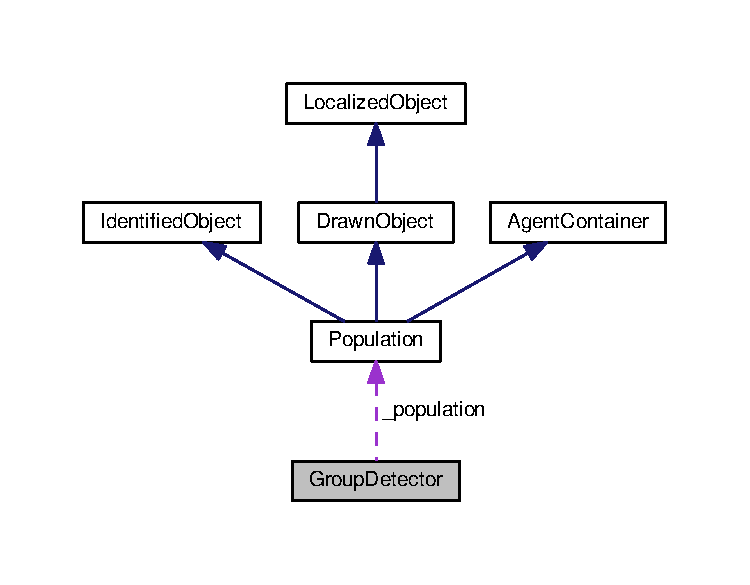
\includegraphics[width=350pt]{classGroupDetector__coll__graph}
\end{center}
\end{figure}
\subsection*{Public Member Functions}
\begin{DoxyCompactItemize}
\item 
\hyperlink{classGroupDetector_a85c950492809247f6ff0649c5101ce81}{Group\+Detector} (\hyperlink{classPopulation}{Population} $\ast$pop)
\begin{DoxyCompactList}\small\item\em Constructor. \end{DoxyCompactList}\item 
virtual \hyperlink{classGroupDetector_a5b44e047c1f6864e665d917ba7da8a51}{$\sim$\+Group\+Detector} ()
\begin{DoxyCompactList}\small\item\em Destructor. \end{DoxyCompactList}\item 
void \hyperlink{classGroupDetector_a4f97c96bbd5c874e788371dffa074001}{detect} ()\hypertarget{classGroupDetector_a4f97c96bbd5c874e788371dffa074001}{}\label{classGroupDetector_a4f97c96bbd5c874e788371dffa074001}

\begin{DoxyCompactList}\small\item\em Find and create every Formations in the \hyperlink{classPopulation}{Population}. \end{DoxyCompactList}\item 
void \hyperlink{classGroupDetector_a8bee5ba0c6e18594eb810e21ee75bac4}{check\+Existing\+Formation} ()\hypertarget{classGroupDetector_a8bee5ba0c6e18594eb810e21ee75bac4}{}\label{classGroupDetector_a8bee5ba0c6e18594eb810e21ee75bac4}

\begin{DoxyCompactList}\small\item\em Check if existing Formations are empty or if \hyperlink{classAgent}{Agent} is alone in a \hyperlink{classFormation}{Formation} and remove them. \end{DoxyCompactList}\end{DoxyCompactItemize}
\subsection*{Protected Attributes}
\begin{DoxyCompactItemize}
\item 
\hyperlink{classPopulation}{Population} $\ast$ \hyperlink{classGroupDetector_a773ce547e63eac75d32d964d70180cd9}{\+\_\+population}\hypertarget{classGroupDetector_a773ce547e63eac75d32d964d70180cd9}{}\label{classGroupDetector_a773ce547e63eac75d32d964d70180cd9}

\begin{DoxyCompactList}\small\item\em The \hyperlink{classPopulation}{Population} processed by the \hyperlink{classGroupDetector}{Group\+Detector}. \end{DoxyCompactList}\item 
int \hyperlink{classGroupDetector_a2cb0f3a229ac96d133f657e306d5d685}{formation\+Id} = 0\hypertarget{classGroupDetector_a2cb0f3a229ac96d133f657e306d5d685}{}\label{classGroupDetector_a2cb0f3a229ac96d133f657e306d5d685}

\begin{DoxyCompactList}\small\item\em The actual increment for unique identifier of the Formations created. \end{DoxyCompactList}\end{DoxyCompactItemize}


\subsection{Detailed Description}
This class is dedicated to process every Agents in the \hyperlink{classPopulation}{Population} and create every \hyperlink{classFormation}{Formation}. 

\begin{DoxyRefDesc}{Todo}
\item[\hyperlink{todo__todo000002}{Todo}]This class should be an interface and actual logic should be implemented has Basic\+Group\+Detector \end{DoxyRefDesc}


\subsection{Constructor \& Destructor Documentation}
\index{Group\+Detector@{Group\+Detector}!Group\+Detector@{Group\+Detector}}
\index{Group\+Detector@{Group\+Detector}!Group\+Detector@{Group\+Detector}}
\subsubsection[{\texorpdfstring{Group\+Detector(\+Population $\ast$pop)}{GroupDetector(Population *pop)}}]{\setlength{\rightskip}{0pt plus 5cm}Group\+Detector\+::\+Group\+Detector (
\begin{DoxyParamCaption}
\item[{{\bf Population} $\ast$}]{pop}
\end{DoxyParamCaption}
)}\hypertarget{classGroupDetector_a85c950492809247f6ff0649c5101ce81}{}\label{classGroupDetector_a85c950492809247f6ff0649c5101ce81}


Constructor. 

Constructor of the \hyperlink{classGroupDetector}{Group\+Detector} class


\begin{DoxyParams}{Parameters}
{\em pop} & \+: The \hyperlink{classPopulation}{Population} that the detector will process \\
\hline
\end{DoxyParams}
\index{Group\+Detector@{Group\+Detector}!````~Group\+Detector@{$\sim$\+Group\+Detector}}
\index{````~Group\+Detector@{$\sim$\+Group\+Detector}!Group\+Detector@{Group\+Detector}}
\subsubsection[{\texorpdfstring{$\sim$\+Group\+Detector()}{~GroupDetector()}}]{\setlength{\rightskip}{0pt plus 5cm}Group\+Detector\+::$\sim$\+Group\+Detector (
\begin{DoxyParamCaption}
{}
\end{DoxyParamCaption}
)\hspace{0.3cm}{\ttfamily [virtual]}}\hypertarget{classGroupDetector_a5b44e047c1f6864e665d917ba7da8a51}{}\label{classGroupDetector_a5b44e047c1f6864e665d917ba7da8a51}


Destructor. 

Destructor of the \hyperlink{classGroupDetector}{Group\+Detector} class, it does not call the related \hyperlink{classPopulation}{Population} destructor 

The documentation for this class was generated from the following files\+:\begin{DoxyCompactItemize}
\item 
src/social\+Processing/\hyperlink{GroupDetector_8h}{Group\+Detector.\+h}\item 
src/social\+Processing/\hyperlink{GroupDetector_8cpp}{Group\+Detector.\+cpp}\end{DoxyCompactItemize}

\hypertarget{classGroupSocialSpace}{}\section{Group\+Social\+Space Class Reference}
\label{classGroupSocialSpace}\index{Group\+Social\+Space@{Group\+Social\+Space}}


This class is an interface to implement representation of a \hyperlink{classGroupSocialSpace}{Group\+Social\+Space}.  




{\ttfamily \#include $<$Group\+Social\+Space.\+h$>$}



Inheritance diagram for Group\+Social\+Space\+:\nopagebreak
\begin{figure}[H]
\begin{center}
\leavevmode
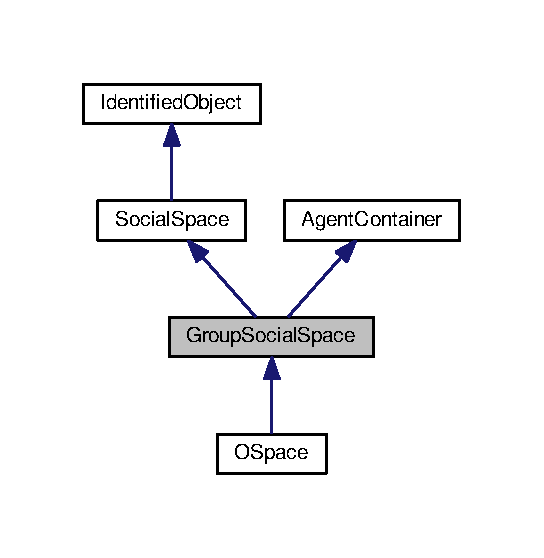
\includegraphics[width=261pt]{classGroupSocialSpace__inherit__graph}
\end{center}
\end{figure}


Collaboration diagram for Group\+Social\+Space\+:\nopagebreak
\begin{figure}[H]
\begin{center}
\leavevmode
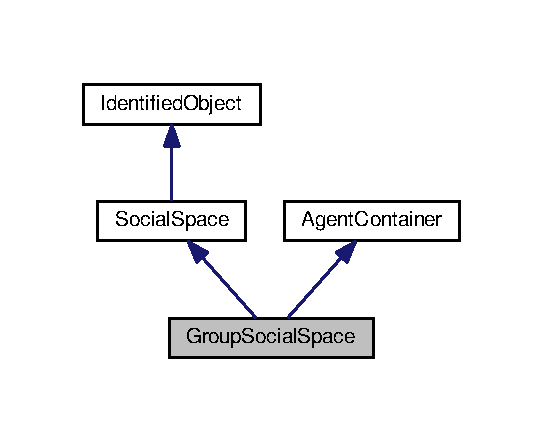
\includegraphics[width=261pt]{classGroupSocialSpace__coll__graph}
\end{center}
\end{figure}
\subsection*{Public Member Functions}
\begin{DoxyCompactItemize}
\item 
\hyperlink{classGroupSocialSpace_af1f690cd933fb5d6272c68e6a0551efa}{Group\+Social\+Space} (int \hyperlink{classIdentifiedObject_ad044a317a9b573a3d1bcd025df166eb5}{id}=0)
\begin{DoxyCompactList}\small\item\em Constructor. \end{DoxyCompactList}\item 
\hyperlink{classGroupSocialSpace_a30f027f4d6ac7c0d0645240cf093d220}{Group\+Social\+Space} (std\+::vector$<$ \hyperlink{classAgent}{Agent} $\ast$ $>$ \&agents, int \hyperlink{classIdentifiedObject_ad044a317a9b573a3d1bcd025df166eb5}{id}=0)
\begin{DoxyCompactList}\small\item\em Constructor. \end{DoxyCompactList}\item 
virtual \hyperlink{classGroupSocialSpace_add59c0e23f9ab6190ca3bf895d754520}{$\sim$\+Group\+Social\+Space} ()
\begin{DoxyCompactList}\small\item\em Destructor. \end{DoxyCompactList}\end{DoxyCompactItemize}
\subsection*{Additional Inherited Members}


\subsection{Detailed Description}
This class is an interface to implement representation of a \hyperlink{classGroupSocialSpace}{Group\+Social\+Space}. 

This class is an interface to implement representation of the \hyperlink{classGroupSocialSpace}{Group\+Social\+Space} of a \hyperlink{classFormation}{Formation} 

\subsection{Constructor \& Destructor Documentation}
\index{Group\+Social\+Space@{Group\+Social\+Space}!Group\+Social\+Space@{Group\+Social\+Space}}
\index{Group\+Social\+Space@{Group\+Social\+Space}!Group\+Social\+Space@{Group\+Social\+Space}}
\subsubsection[{\texorpdfstring{Group\+Social\+Space(int id=0)}{GroupSocialSpace(int id=0)}}]{\setlength{\rightskip}{0pt plus 5cm}Group\+Social\+Space\+::\+Group\+Social\+Space (
\begin{DoxyParamCaption}
\item[{int}]{id = {\ttfamily 0}}
\end{DoxyParamCaption}
)}\hypertarget{classGroupSocialSpace_af1f690cd933fb5d6272c68e6a0551efa}{}\label{classGroupSocialSpace_af1f690cd933fb5d6272c68e6a0551efa}


Constructor. 

Constructor of the \hyperlink{classGroupSocialSpace}{Group\+Social\+Space} class, with no \hyperlink{classAgent}{Agent}


\begin{DoxyParams}{Parameters}
{\em id} & \+: The unique identifier of the \hyperlink{classGroupSocialSpace}{Group\+Social\+Space} \\
\hline
\end{DoxyParams}
\index{Group\+Social\+Space@{Group\+Social\+Space}!Group\+Social\+Space@{Group\+Social\+Space}}
\index{Group\+Social\+Space@{Group\+Social\+Space}!Group\+Social\+Space@{Group\+Social\+Space}}
\subsubsection[{\texorpdfstring{Group\+Social\+Space(std\+::vector$<$ Agent $\ast$ $>$ \&agents, int id=0)}{GroupSocialSpace(std::vector< Agent * > &agents, int id=0)}}]{\setlength{\rightskip}{0pt plus 5cm}Group\+Social\+Space\+::\+Group\+Social\+Space (
\begin{DoxyParamCaption}
\item[{std\+::vector$<$ {\bf Agent} $\ast$ $>$ \&}]{agents, }
\item[{int}]{id = {\ttfamily 0}}
\end{DoxyParamCaption}
)}\hypertarget{classGroupSocialSpace_a30f027f4d6ac7c0d0645240cf093d220}{}\label{classGroupSocialSpace_a30f027f4d6ac7c0d0645240cf093d220}


Constructor. 

Constructor of the \hyperlink{classGroupSocialSpace}{Group\+Social\+Space} class, for the Agents in parameter


\begin{DoxyParams}{Parameters}
{\em agents} & \+: The Agents related to the \hyperlink{classGroupSocialSpace}{Group\+Social\+Space} \\
\hline
{\em id} & \+: The unique identifier of the \hyperlink{classGroupSocialSpace}{Group\+Social\+Space} \\
\hline
\end{DoxyParams}
\index{Group\+Social\+Space@{Group\+Social\+Space}!````~Group\+Social\+Space@{$\sim$\+Group\+Social\+Space}}
\index{````~Group\+Social\+Space@{$\sim$\+Group\+Social\+Space}!Group\+Social\+Space@{Group\+Social\+Space}}
\subsubsection[{\texorpdfstring{$\sim$\+Group\+Social\+Space()}{~GroupSocialSpace()}}]{\setlength{\rightskip}{0pt plus 5cm}Group\+Social\+Space\+::$\sim$\+Group\+Social\+Space (
\begin{DoxyParamCaption}
{}
\end{DoxyParamCaption}
)\hspace{0.3cm}{\ttfamily [virtual]}}\hypertarget{classGroupSocialSpace_add59c0e23f9ab6190ca3bf895d754520}{}\label{classGroupSocialSpace_add59c0e23f9ab6190ca3bf895d754520}


Destructor. 

Destructor of the \hyperlink{classGroupSocialSpace}{Group\+Social\+Space} class 

The documentation for this class was generated from the following files\+:\begin{DoxyCompactItemize}
\item 
src/social\+Space/\hyperlink{GroupSocialSpace_8h}{Group\+Social\+Space.\+h}\item 
src/social\+Space/Group\+Social\+Space.\+cpp\end{DoxyCompactItemize}

\hypertarget{classGui}{}\section{Gui Class Reference}
\label{classGui}\index{Gui@{Gui}}


Graphical User Interface.  




{\ttfamily \#include $<$Gui.\+h$>$}

\subsection*{Public Member Functions}
\begin{DoxyCompactItemize}
\item 
void {\bfseries draw} ()\hypertarget{classGui_a51dbe7d00fcc9154b2ed1b181668d2db}{}\label{classGui_a51dbe7d00fcc9154b2ed1b181668d2db}

\item 
void {\bfseries button\+Pressed} ()\hypertarget{classGui_a012766edbe7b63bb0a334d0dc0a20acf}{}\label{classGui_a012766edbe7b63bb0a334d0dc0a20acf}

\item 
void {\bfseries toggle\+Pressed} (bool \&pressed)\hypertarget{classGui_abcd8b5e32f522560f4f8672a9a30b174}{}\label{classGui_abcd8b5e32f522560f4f8672a9a30b174}

\item 
void {\bfseries exit} ()\hypertarget{classGui_a6748646c37e27710a82d5413b4169469}{}\label{classGui_a6748646c37e27710a82d5413b4169469}

\end{DoxyCompactItemize}
\subsection*{Public Attributes}
\begin{DoxyCompactItemize}
\item 
ofx\+Button {\bfseries button}\hypertarget{classGui_a8179cc8b574ae41c79b5df59ceac9505}{}\label{classGui_a8179cc8b574ae41c79b5df59ceac9505}

\item 
ofx\+Toggle {\bfseries toggle}\hypertarget{classGui_a5982f21b03c99e1acb237cf1e9eae13e}{}\label{classGui_a5982f21b03c99e1acb237cf1e9eae13e}

\item 
ofx\+Panel {\bfseries gui}\hypertarget{classGui_aa383c046993cb66c31d30819c3a4addd}{}\label{classGui_aa383c046993cb66c31d30819c3a4addd}

\end{DoxyCompactItemize}


\subsection{Detailed Description}
Graphical User Interface. 

The documentation for this class was generated from the following files\+:\begin{DoxyCompactItemize}
\item 
src/Gui.\+h\item 
src/Gui.\+cpp\end{DoxyCompactItemize}

\hypertarget{classIdentifiedObject}{}\section{Identified\+Object Class Reference}
\label{classIdentifiedObject}\index{Identified\+Object@{Identified\+Object}}


This class is an interface for class that need a unique identifier.  




{\ttfamily \#include $<$Identified\+Object.\+h$>$}



Inheritance diagram for Identified\+Object\+:\nopagebreak
\begin{figure}[H]
\begin{center}
\leavevmode
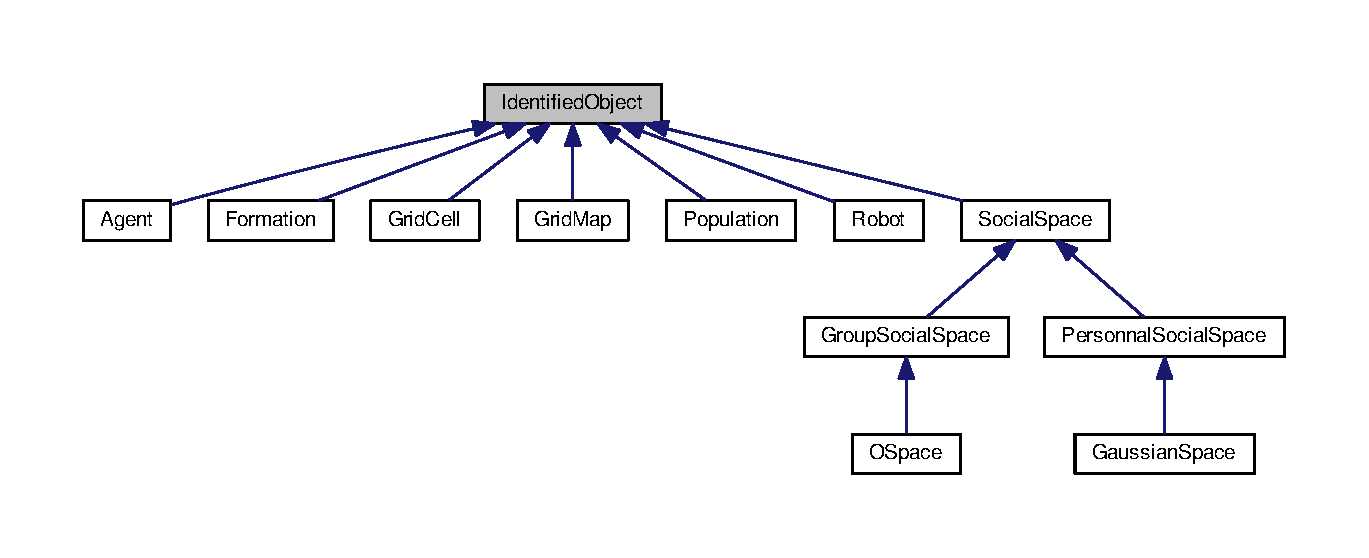
\includegraphics[width=350pt]{classIdentifiedObject__inherit__graph}
\end{center}
\end{figure}
\subsection*{Public Member Functions}
\begin{DoxyCompactItemize}
\item 
\hyperlink{classIdentifiedObject_ab2b3eaf77f6ff94f619478d0f20dd5c1}{Identified\+Object} (unsigned int \hyperlink{classIdentifiedObject_ad044a317a9b573a3d1bcd025df166eb5}{id}=0)
\begin{DoxyCompactList}\small\item\em Constructor. \end{DoxyCompactList}\item 
virtual \hyperlink{classIdentifiedObject_af240a574a25906024375725985ef46b4}{$\sim$\+Identified\+Object} ()
\begin{DoxyCompactList}\small\item\em Destructor. \end{DoxyCompactList}\item 
unsigned int \hyperlink{classIdentifiedObject_a1fdb1d89faff5712c9016c4fdd55bf47}{get\+Id} () const 
\begin{DoxyCompactList}\small\item\em Simple getter. \end{DoxyCompactList}\item 
void \hyperlink{classIdentifiedObject_a48cbaa2561de7a401bf01a0541c596ff}{set\+Id} (unsigned int \hyperlink{classIdentifiedObject_ad044a317a9b573a3d1bcd025df166eb5}{id})
\begin{DoxyCompactList}\small\item\em Simpler setter. \end{DoxyCompactList}\end{DoxyCompactItemize}
\subsection*{Protected Attributes}
\begin{DoxyCompactItemize}
\item 
unsigned int \hyperlink{classIdentifiedObject_ad044a317a9b573a3d1bcd025df166eb5}{id}\hypertarget{classIdentifiedObject_ad044a317a9b573a3d1bcd025df166eb5}{}\label{classIdentifiedObject_ad044a317a9b573a3d1bcd025df166eb5}

\begin{DoxyCompactList}\small\item\em The unique identifier. \end{DoxyCompactList}\end{DoxyCompactItemize}


\subsection{Detailed Description}
This class is an interface for class that need a unique identifier. 

\subsection{Constructor \& Destructor Documentation}
\index{Identified\+Object@{Identified\+Object}!Identified\+Object@{Identified\+Object}}
\index{Identified\+Object@{Identified\+Object}!Identified\+Object@{Identified\+Object}}
\subsubsection[{\texorpdfstring{Identified\+Object(unsigned int id=0)}{IdentifiedObject(unsigned int id=0)}}]{\setlength{\rightskip}{0pt plus 5cm}Identified\+Object\+::\+Identified\+Object (
\begin{DoxyParamCaption}
\item[{unsigned int}]{id = {\ttfamily 0}}
\end{DoxyParamCaption}
)}\hypertarget{classIdentifiedObject_ab2b3eaf77f6ff94f619478d0f20dd5c1}{}\label{classIdentifiedObject_ab2b3eaf77f6ff94f619478d0f20dd5c1}


Constructor. 

Constructor of the \hyperlink{classIdentifiedObject}{Identified\+Object} class


\begin{DoxyParams}{Parameters}
{\em id} & \+: The unique identifier of the object \\
\hline
\end{DoxyParams}
\index{Identified\+Object@{Identified\+Object}!````~Identified\+Object@{$\sim$\+Identified\+Object}}
\index{````~Identified\+Object@{$\sim$\+Identified\+Object}!Identified\+Object@{Identified\+Object}}
\subsubsection[{\texorpdfstring{$\sim$\+Identified\+Object()}{~IdentifiedObject()}}]{\setlength{\rightskip}{0pt plus 5cm}Identified\+Object\+::$\sim$\+Identified\+Object (
\begin{DoxyParamCaption}
{}
\end{DoxyParamCaption}
)\hspace{0.3cm}{\ttfamily [virtual]}}\hypertarget{classIdentifiedObject_af240a574a25906024375725985ef46b4}{}\label{classIdentifiedObject_af240a574a25906024375725985ef46b4}


Destructor. 

Destructor of the \hyperlink{classIdentifiedObject}{Identified\+Object} class 

\subsection{Member Function Documentation}
\index{Identified\+Object@{Identified\+Object}!get\+Id@{get\+Id}}
\index{get\+Id@{get\+Id}!Identified\+Object@{Identified\+Object}}
\subsubsection[{\texorpdfstring{get\+Id() const }{getId() const }}]{\setlength{\rightskip}{0pt plus 5cm}unsigned int Identified\+Object\+::get\+Id (
\begin{DoxyParamCaption}
{}
\end{DoxyParamCaption}
) const}\hypertarget{classIdentifiedObject_a1fdb1d89faff5712c9016c4fdd55bf47}{}\label{classIdentifiedObject_a1fdb1d89faff5712c9016c4fdd55bf47}


Simple getter. 

\begin{DoxyReturn}{Returns}
id 
\end{DoxyReturn}
\index{Identified\+Object@{Identified\+Object}!set\+Id@{set\+Id}}
\index{set\+Id@{set\+Id}!Identified\+Object@{Identified\+Object}}
\subsubsection[{\texorpdfstring{set\+Id(unsigned int id)}{setId(unsigned int id)}}]{\setlength{\rightskip}{0pt plus 5cm}void Identified\+Object\+::set\+Id (
\begin{DoxyParamCaption}
\item[{unsigned int}]{id}
\end{DoxyParamCaption}
)}\hypertarget{classIdentifiedObject_a48cbaa2561de7a401bf01a0541c596ff}{}\label{classIdentifiedObject_a48cbaa2561de7a401bf01a0541c596ff}


Simpler setter. 


\begin{DoxyParams}{Parameters}
{\em id} & \\
\hline
\end{DoxyParams}


The documentation for this class was generated from the following files\+:\begin{DoxyCompactItemize}
\item 
src/generic\+Type/\hyperlink{IdentifiedObject_8h}{Identified\+Object.\+h}\item 
src/generic\+Type/\hyperlink{IdentifiedObject_8cpp}{Identified\+Object.\+cpp}\end{DoxyCompactItemize}

\hypertarget{classLocalizedObject}{}\section{Localized\+Object Class Reference}
\label{classLocalizedObject}\index{Localized\+Object@{Localized\+Object}}


This class is an interface for object that are localized in real \hyperlink{classWorld}{World}.  




{\ttfamily \#include $<$Localized\+Object.\+h$>$}



Inheritance diagram for Localized\+Object\+:\nopagebreak
\begin{figure}[H]
\begin{center}
\leavevmode
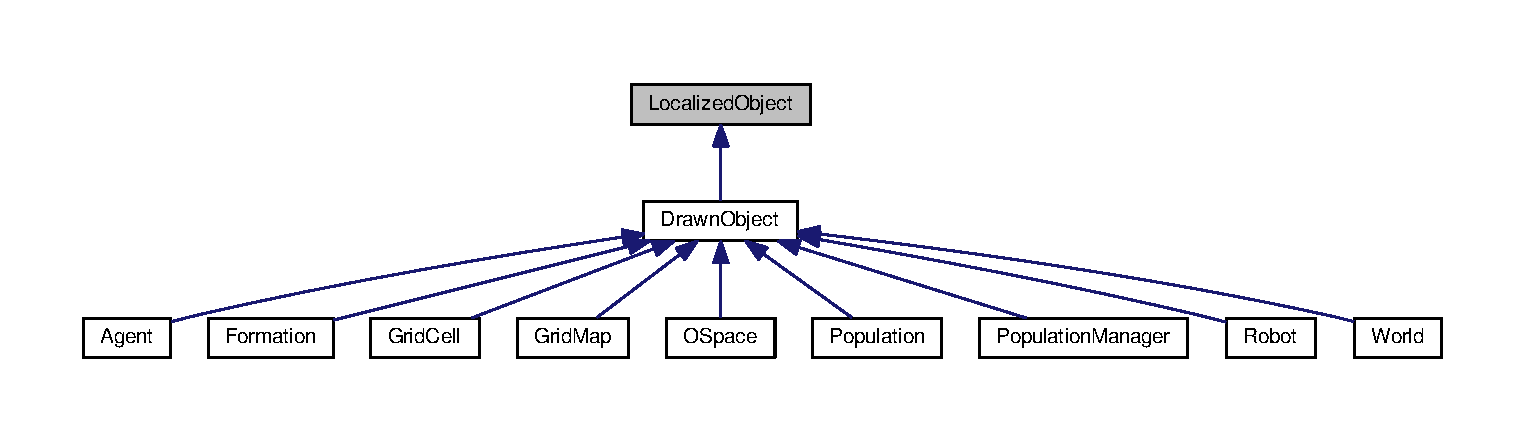
\includegraphics[width=350pt]{classLocalizedObject__inherit__graph}
\end{center}
\end{figure}
\subsection*{Public Member Functions}
\begin{DoxyCompactItemize}
\item 
\hyperlink{classLocalizedObject_a85c2aba0c93b4d90b9e001409d6a5381}{Localized\+Object} (Vector3d \hyperlink{classLocalizedObject_a340834deefc9e5c39da1f26c4ebf4f8c}{position}=Vector3d(), double \hyperlink{classLocalizedObject_aa5f7b070b6dc97a64a90797a0bca56e2}{theta}=0)
\begin{DoxyCompactList}\small\item\em Constructor. \end{DoxyCompactList}\item 
virtual \hyperlink{classLocalizedObject_a1425438490ec7cd508721b9ccaef7a80}{$\sim$\+Localized\+Object} ()
\begin{DoxyCompactList}\small\item\em Destructor. \end{DoxyCompactList}\item 
Vector3d \hyperlink{classLocalizedObject_ab3a9262ca2086b812166a5b23df0a34c}{get\+Direction} ()
\begin{DoxyCompactList}\small\item\em Compute the direction vector of the object from its angle. \end{DoxyCompactList}\item 
double \hyperlink{classLocalizedObject_a5fec63cd061189992f011237a62c81b2}{getX} () const 
\begin{DoxyCompactList}\small\item\em Simple getter. \end{DoxyCompactList}\item 
void \hyperlink{classLocalizedObject_a53154ec51dcbf7d200f8f6f09c65f247}{setX} (double x)
\begin{DoxyCompactList}\small\item\em Simple setter. \end{DoxyCompactList}\item 
double \hyperlink{classLocalizedObject_a406d1b48a67b1d6bbfc98d6b57c7f24e}{getY} () const 
\begin{DoxyCompactList}\small\item\em Simple getter. \end{DoxyCompactList}\item 
void \hyperlink{classLocalizedObject_a6d9bf8b47e887c48d126fa367d1c084b}{setY} (double y)
\begin{DoxyCompactList}\small\item\em Simple setter. \end{DoxyCompactList}\item 
Vector3d \hyperlink{classLocalizedObject_a711da75e218c7cc64b57088d3c1a8c73}{get\+Position} () const 
\begin{DoxyCompactList}\small\item\em Simple getter. \end{DoxyCompactList}\item 
void \hyperlink{classLocalizedObject_adbdcf655524574dc3c1a4d3f9adfd259}{set\+Position} (Vector3d \hyperlink{classLocalizedObject_a340834deefc9e5c39da1f26c4ebf4f8c}{position})
\begin{DoxyCompactList}\small\item\em Simple setter. \end{DoxyCompactList}\item 
double \hyperlink{classLocalizedObject_a9a5927a035686eccc401aa2b1e8d0595}{get\+Theta} () const 
\begin{DoxyCompactList}\small\item\em Simple getter. \end{DoxyCompactList}\item 
void \hyperlink{classLocalizedObject_ac23f5d3d6afebb24e5b52c71197f3551}{set\+Theta} (double \hyperlink{classLocalizedObject_aa5f7b070b6dc97a64a90797a0bca56e2}{theta})
\begin{DoxyCompactList}\small\item\em Simple setter. \end{DoxyCompactList}\end{DoxyCompactItemize}
\subsection*{Protected Attributes}
\begin{DoxyCompactItemize}
\item 
Vector3d \hyperlink{classLocalizedObject_a340834deefc9e5c39da1f26c4ebf4f8c}{position}\hypertarget{classLocalizedObject_a340834deefc9e5c39da1f26c4ebf4f8c}{}\label{classLocalizedObject_a340834deefc9e5c39da1f26c4ebf4f8c}

\begin{DoxyCompactList}\small\item\em The position of the object. \end{DoxyCompactList}\item 
double \hyperlink{classLocalizedObject_aa5f7b070b6dc97a64a90797a0bca56e2}{theta}\hypertarget{classLocalizedObject_aa5f7b070b6dc97a64a90797a0bca56e2}{}\label{classLocalizedObject_aa5f7b070b6dc97a64a90797a0bca56e2}

\begin{DoxyCompactList}\small\item\em The angle of the object relative to X axis (1,0,0) (arround Z axis (0,0,1)) and in radian normalized between \mbox{[}0,2\+PI\mbox{]}. \end{DoxyCompactList}\end{DoxyCompactItemize}


\subsection{Detailed Description}
This class is an interface for object that are localized in real \hyperlink{classWorld}{World}. 

This class is an interface for object that are localize in real \hyperlink{classWorld}{World} with x, y, z and Theta coordinates 

\subsection{Constructor \& Destructor Documentation}
\index{Localized\+Object@{Localized\+Object}!Localized\+Object@{Localized\+Object}}
\index{Localized\+Object@{Localized\+Object}!Localized\+Object@{Localized\+Object}}
\subsubsection[{\texorpdfstring{Localized\+Object(\+Vector3d position=\+Vector3d(), double theta=0)}{LocalizedObject(Vector3d position=Vector3d(), double theta=0)}}]{\setlength{\rightskip}{0pt plus 5cm}Localized\+Object\+::\+Localized\+Object (
\begin{DoxyParamCaption}
\item[{Vector3d}]{position = {\ttfamily Vector3d()}, }
\item[{double}]{theta = {\ttfamily 0}}
\end{DoxyParamCaption}
)}\hypertarget{classLocalizedObject_a85c2aba0c93b4d90b9e001409d6a5381}{}\label{classLocalizedObject_a85c2aba0c93b4d90b9e001409d6a5381}


Constructor. 

Constructor of the \hyperlink{classLocalizedObject}{Localized\+Object} class


\begin{DoxyParams}{Parameters}
{\em position} & \+: The initial position of the object \\
\hline
{\em theta} & \+: The initial angle of the object relative to X axis in radian \\
\hline
\end{DoxyParams}
\index{Localized\+Object@{Localized\+Object}!````~Localized\+Object@{$\sim$\+Localized\+Object}}
\index{````~Localized\+Object@{$\sim$\+Localized\+Object}!Localized\+Object@{Localized\+Object}}
\subsubsection[{\texorpdfstring{$\sim$\+Localized\+Object()}{~LocalizedObject()}}]{\setlength{\rightskip}{0pt plus 5cm}Localized\+Object\+::$\sim$\+Localized\+Object (
\begin{DoxyParamCaption}
{}
\end{DoxyParamCaption}
)\hspace{0.3cm}{\ttfamily [virtual]}}\hypertarget{classLocalizedObject_a1425438490ec7cd508721b9ccaef7a80}{}\label{classLocalizedObject_a1425438490ec7cd508721b9ccaef7a80}


Destructor. 

Destructor of the \hyperlink{classLocalizedObject}{Localized\+Object} class 

\subsection{Member Function Documentation}
\index{Localized\+Object@{Localized\+Object}!get\+Direction@{get\+Direction}}
\index{get\+Direction@{get\+Direction}!Localized\+Object@{Localized\+Object}}
\subsubsection[{\texorpdfstring{get\+Direction()}{getDirection()}}]{\setlength{\rightskip}{0pt plus 5cm}Vector3d Localized\+Object\+::get\+Direction (
\begin{DoxyParamCaption}
{}
\end{DoxyParamCaption}
)}\hypertarget{classLocalizedObject_ab3a9262ca2086b812166a5b23df0a34c}{}\label{classLocalizedObject_ab3a9262ca2086b812166a5b23df0a34c}


Compute the direction vector of the object from its angle. 

\begin{DoxyReturn}{Returns}
The direction Vector3d 
\end{DoxyReturn}
\index{Localized\+Object@{Localized\+Object}!get\+Position@{get\+Position}}
\index{get\+Position@{get\+Position}!Localized\+Object@{Localized\+Object}}
\subsubsection[{\texorpdfstring{get\+Position() const }{getPosition() const }}]{\setlength{\rightskip}{0pt plus 5cm}Vector3d Localized\+Object\+::get\+Position (
\begin{DoxyParamCaption}
{}
\end{DoxyParamCaption}
) const}\hypertarget{classLocalizedObject_a711da75e218c7cc64b57088d3c1a8c73}{}\label{classLocalizedObject_a711da75e218c7cc64b57088d3c1a8c73}


Simple getter. 

\begin{DoxyReturn}{Returns}
position 
\end{DoxyReturn}
\index{Localized\+Object@{Localized\+Object}!get\+Theta@{get\+Theta}}
\index{get\+Theta@{get\+Theta}!Localized\+Object@{Localized\+Object}}
\subsubsection[{\texorpdfstring{get\+Theta() const }{getTheta() const }}]{\setlength{\rightskip}{0pt plus 5cm}double Localized\+Object\+::get\+Theta (
\begin{DoxyParamCaption}
{}
\end{DoxyParamCaption}
) const}\hypertarget{classLocalizedObject_a9a5927a035686eccc401aa2b1e8d0595}{}\label{classLocalizedObject_a9a5927a035686eccc401aa2b1e8d0595}


Simple getter. 

\begin{DoxyReturn}{Returns}
theta 
\end{DoxyReturn}
\index{Localized\+Object@{Localized\+Object}!getX@{getX}}
\index{getX@{getX}!Localized\+Object@{Localized\+Object}}
\subsubsection[{\texorpdfstring{get\+X() const }{getX() const }}]{\setlength{\rightskip}{0pt plus 5cm}double Localized\+Object\+::getX (
\begin{DoxyParamCaption}
{}
\end{DoxyParamCaption}
) const}\hypertarget{classLocalizedObject_a5fec63cd061189992f011237a62c81b2}{}\label{classLocalizedObject_a5fec63cd061189992f011237a62c81b2}


Simple getter. 

\begin{DoxyReturn}{Returns}
X coordinate of the position vector 
\end{DoxyReturn}
\index{Localized\+Object@{Localized\+Object}!getY@{getY}}
\index{getY@{getY}!Localized\+Object@{Localized\+Object}}
\subsubsection[{\texorpdfstring{get\+Y() const }{getY() const }}]{\setlength{\rightskip}{0pt plus 5cm}double Localized\+Object\+::getY (
\begin{DoxyParamCaption}
{}
\end{DoxyParamCaption}
) const}\hypertarget{classLocalizedObject_a406d1b48a67b1d6bbfc98d6b57c7f24e}{}\label{classLocalizedObject_a406d1b48a67b1d6bbfc98d6b57c7f24e}


Simple getter. 

\begin{DoxyReturn}{Returns}
Y coordinate of the position vector 
\end{DoxyReturn}
\index{Localized\+Object@{Localized\+Object}!set\+Position@{set\+Position}}
\index{set\+Position@{set\+Position}!Localized\+Object@{Localized\+Object}}
\subsubsection[{\texorpdfstring{set\+Position(\+Vector3d position)}{setPosition(Vector3d position)}}]{\setlength{\rightskip}{0pt plus 5cm}void Localized\+Object\+::set\+Position (
\begin{DoxyParamCaption}
\item[{Vector3d}]{position}
\end{DoxyParamCaption}
)}\hypertarget{classLocalizedObject_adbdcf655524574dc3c1a4d3f9adfd259}{}\label{classLocalizedObject_adbdcf655524574dc3c1a4d3f9adfd259}


Simple setter. 


\begin{DoxyParams}{Parameters}
{\em position} & \\
\hline
\end{DoxyParams}
\index{Localized\+Object@{Localized\+Object}!set\+Theta@{set\+Theta}}
\index{set\+Theta@{set\+Theta}!Localized\+Object@{Localized\+Object}}
\subsubsection[{\texorpdfstring{set\+Theta(double theta)}{setTheta(double theta)}}]{\setlength{\rightskip}{0pt plus 5cm}void Localized\+Object\+::set\+Theta (
\begin{DoxyParamCaption}
\item[{double}]{theta}
\end{DoxyParamCaption}
)}\hypertarget{classLocalizedObject_ac23f5d3d6afebb24e5b52c71197f3551}{}\label{classLocalizedObject_ac23f5d3d6afebb24e5b52c71197f3551}


Simple setter. 


\begin{DoxyParams}{Parameters}
{\em theta} & \\
\hline
\end{DoxyParams}
\index{Localized\+Object@{Localized\+Object}!setX@{setX}}
\index{setX@{setX}!Localized\+Object@{Localized\+Object}}
\subsubsection[{\texorpdfstring{set\+X(double x)}{setX(double x)}}]{\setlength{\rightskip}{0pt plus 5cm}void Localized\+Object\+::setX (
\begin{DoxyParamCaption}
\item[{double}]{x}
\end{DoxyParamCaption}
)}\hypertarget{classLocalizedObject_a53154ec51dcbf7d200f8f6f09c65f247}{}\label{classLocalizedObject_a53154ec51dcbf7d200f8f6f09c65f247}


Simple setter. 


\begin{DoxyParams}{Parameters}
{\em x} & \\
\hline
\end{DoxyParams}
\index{Localized\+Object@{Localized\+Object}!setY@{setY}}
\index{setY@{setY}!Localized\+Object@{Localized\+Object}}
\subsubsection[{\texorpdfstring{set\+Y(double y)}{setY(double y)}}]{\setlength{\rightskip}{0pt plus 5cm}void Localized\+Object\+::setY (
\begin{DoxyParamCaption}
\item[{double}]{y}
\end{DoxyParamCaption}
)}\hypertarget{classLocalizedObject_a6d9bf8b47e887c48d126fa367d1c084b}{}\label{classLocalizedObject_a6d9bf8b47e887c48d126fa367d1c084b}


Simple setter. 


\begin{DoxyParams}{Parameters}
{\em y} & \\
\hline
\end{DoxyParams}


The documentation for this class was generated from the following files\+:\begin{DoxyCompactItemize}
\item 
src/generic\+Type/\hyperlink{LocalizedObject_8h}{Localized\+Object.\+h}\item 
src/generic\+Type/\hyperlink{LocalizedObject_8cpp}{Localized\+Object.\+cpp}\end{DoxyCompactItemize}

\hypertarget{classofApp}{}\section{of\+App Class Reference}
\label{classofApp}\index{of\+App@{of\+App}}


The Openframeworks main class.  




{\ttfamily \#include $<$of\+App.\+h$>$}



Inheritance diagram for of\+App\+:\nopagebreak
\begin{figure}[H]
\begin{center}
\leavevmode
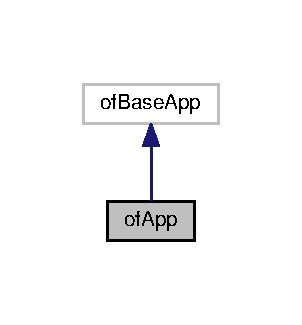
\includegraphics[width=145pt]{classofApp__inherit__graph}
\end{center}
\end{figure}


Collaboration diagram for of\+App\+:\nopagebreak
\begin{figure}[H]
\begin{center}
\leavevmode
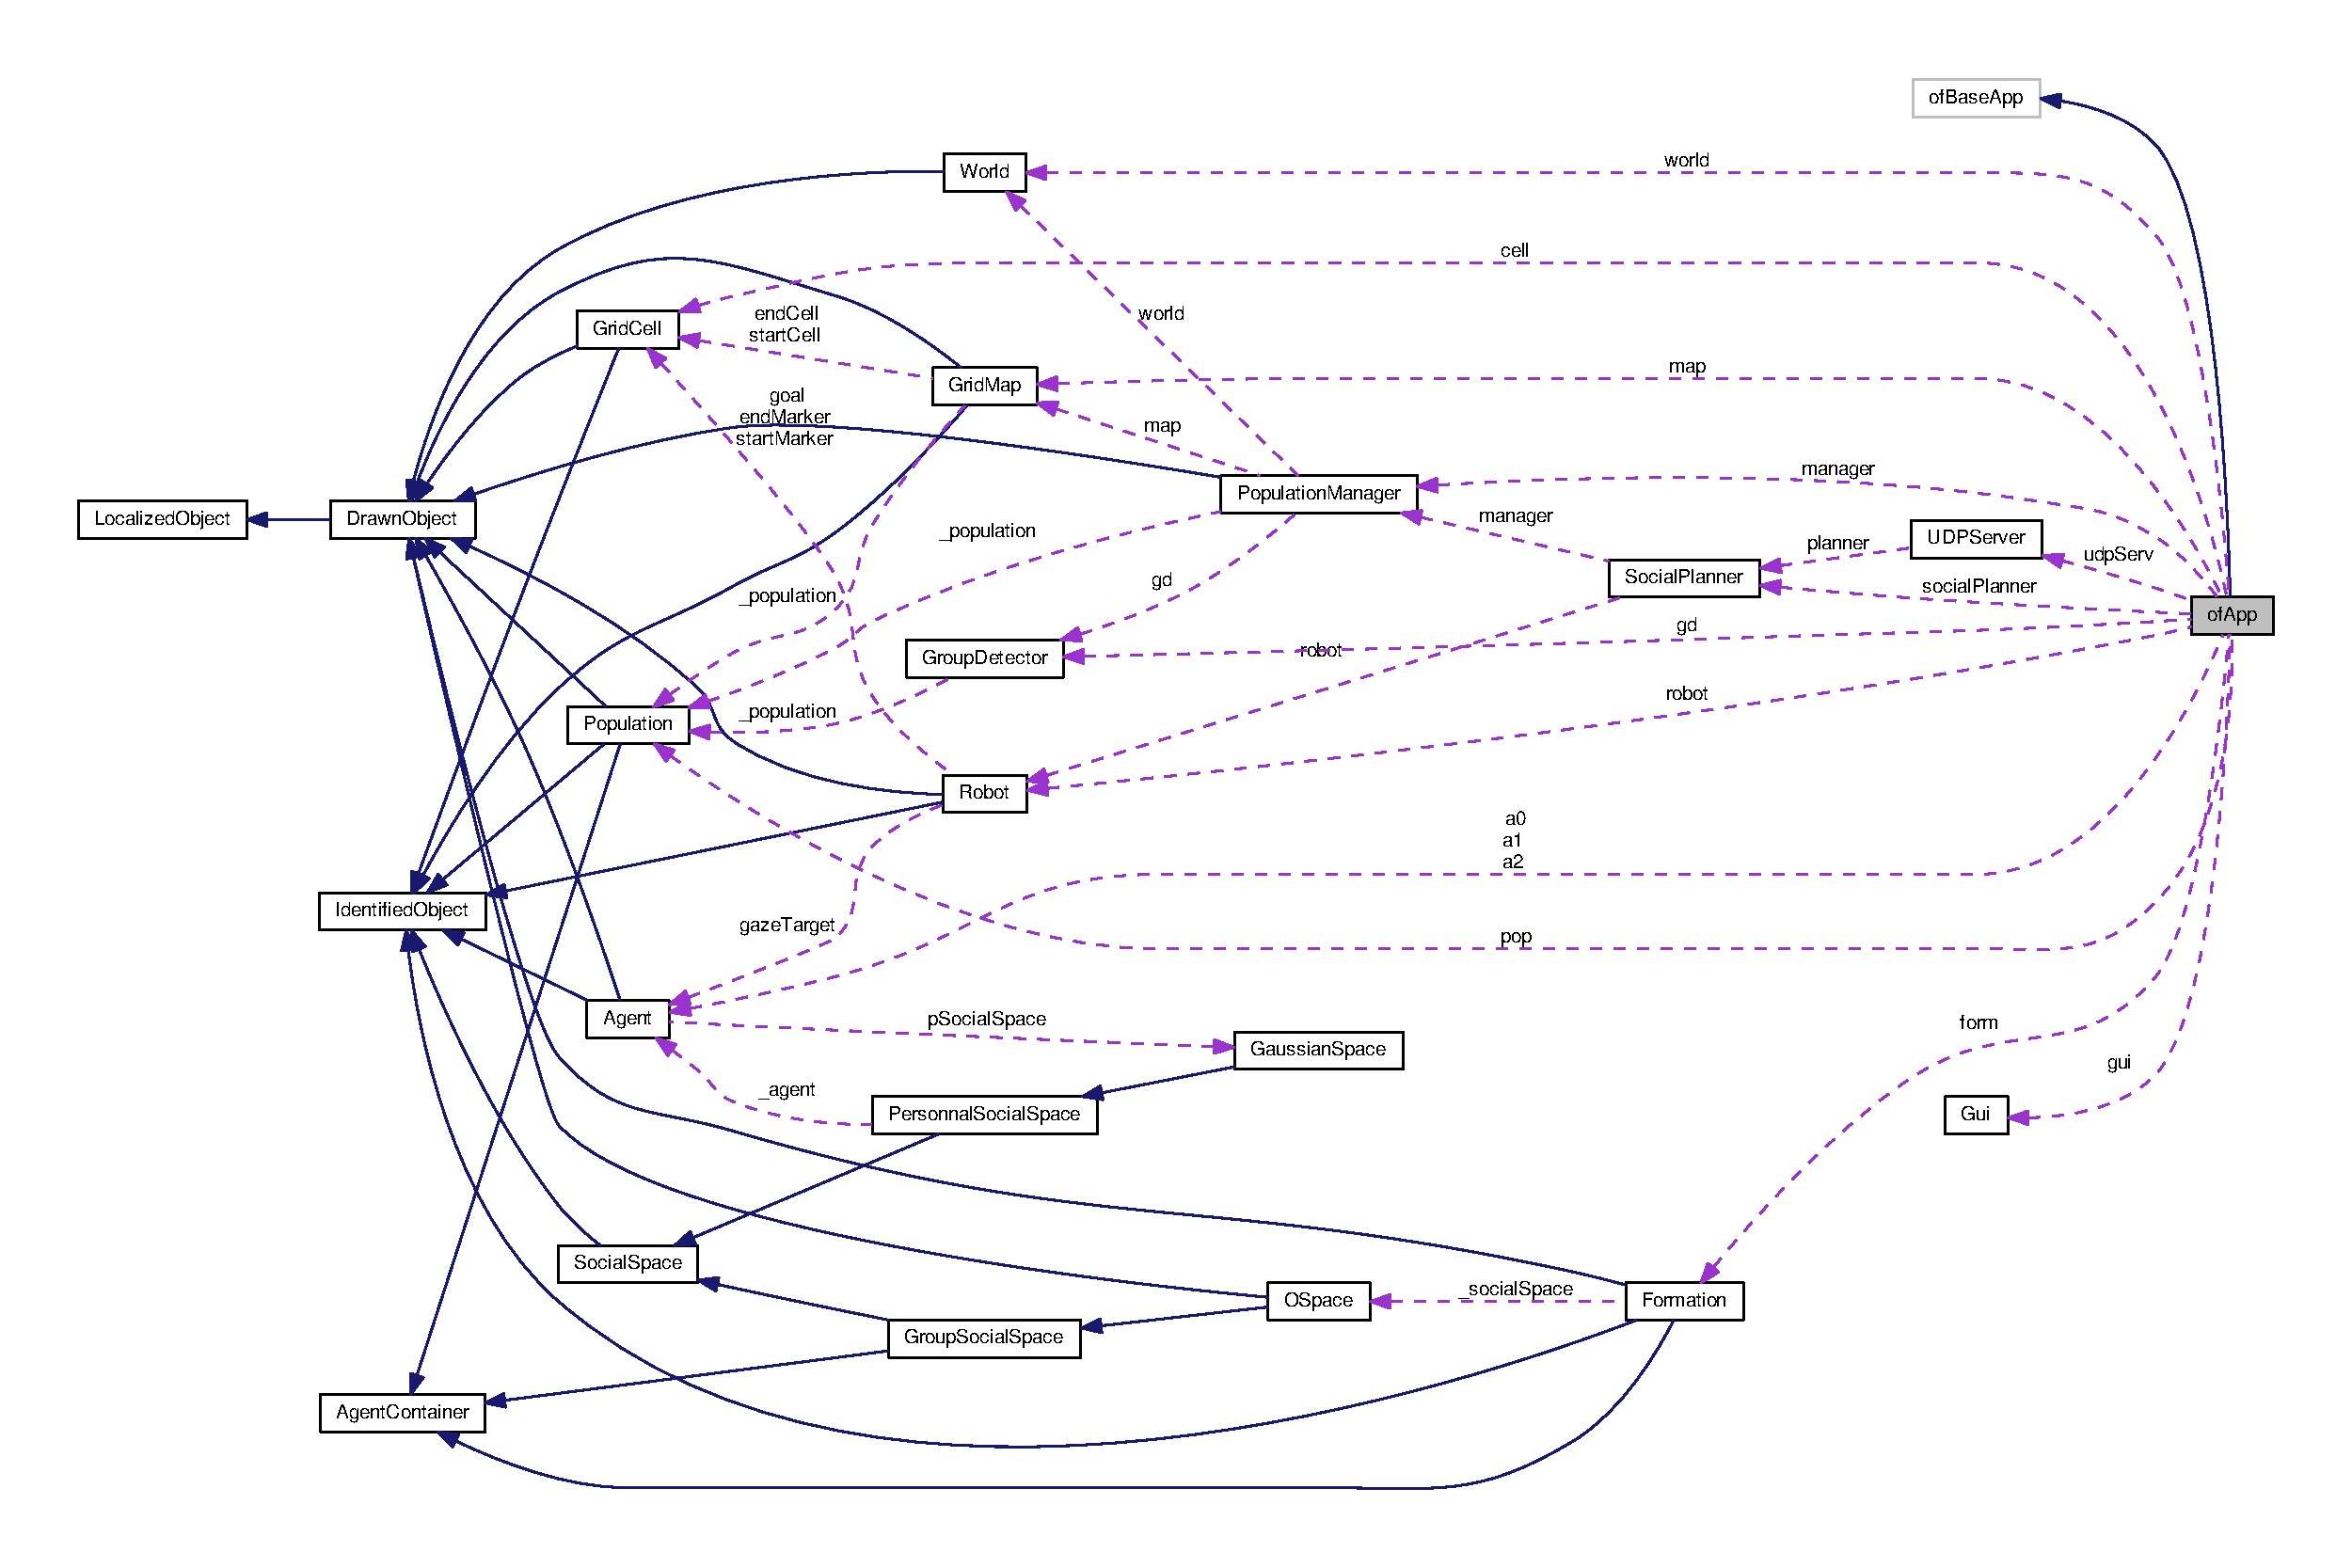
\includegraphics[width=350pt]{classofApp__coll__graph}
\end{center}
\end{figure}
\subsection*{Public Member Functions}
\begin{DoxyCompactItemize}
\item 
void {\bfseries setup} ()\hypertarget{classofApp_af68eaa1366244f7a541cd08e02199c12}{}\label{classofApp_af68eaa1366244f7a541cd08e02199c12}

\item 
void {\bfseries update} ()\hypertarget{classofApp_afef41ea4aee5a22ea530afba33ae7a7b}{}\label{classofApp_afef41ea4aee5a22ea530afba33ae7a7b}

\item 
void {\bfseries draw} ()\hypertarget{classofApp_a75dd45437b9e317db73d8daef1ad49f8}{}\label{classofApp_a75dd45437b9e317db73d8daef1ad49f8}

\item 
void {\bfseries key\+Pressed} (int key)\hypertarget{classofApp_a957d3197364bbac8e67eaa4f15b28ad3}{}\label{classofApp_a957d3197364bbac8e67eaa4f15b28ad3}

\item 
void {\bfseries key\+Released} (int key)\hypertarget{classofApp_aa1503a87453bcfdd395fe4acca5d91a0}{}\label{classofApp_aa1503a87453bcfdd395fe4acca5d91a0}

\item 
void {\bfseries mouse\+Moved} (int x, int y)\hypertarget{classofApp_a158b41a606310db4633fdb817b21047c}{}\label{classofApp_a158b41a606310db4633fdb817b21047c}

\item 
void {\bfseries mouse\+Dragged} (int x, int y, int button)\hypertarget{classofApp_a1ec53d1be799dc275806ff6c6548cd83}{}\label{classofApp_a1ec53d1be799dc275806ff6c6548cd83}

\item 
void {\bfseries mouse\+Pressed} (int x, int y, int button)\hypertarget{classofApp_a2c2ea9c160231e55424dfd98466ef27d}{}\label{classofApp_a2c2ea9c160231e55424dfd98466ef27d}

\item 
void {\bfseries mouse\+Released} (int x, int y, int button)\hypertarget{classofApp_aa3131f1554fc49eaa9ee0f284e48129b}{}\label{classofApp_aa3131f1554fc49eaa9ee0f284e48129b}

\item 
void {\bfseries mouse\+Entered} (int x, int y)\hypertarget{classofApp_aa54e1ffc660d8261617c369c9b29c432}{}\label{classofApp_aa54e1ffc660d8261617c369c9b29c432}

\item 
void {\bfseries mouse\+Exited} (int x, int y)\hypertarget{classofApp_ad31f79798b598551792dab6ba7c61fd1}{}\label{classofApp_ad31f79798b598551792dab6ba7c61fd1}

\item 
void {\bfseries window\+Resized} (int w, int h)\hypertarget{classofApp_ae4dc1ec1513dcbe48bc78a5e4c3fac0f}{}\label{classofApp_ae4dc1ec1513dcbe48bc78a5e4c3fac0f}

\item 
void {\bfseries drag\+Event} (of\+Drag\+Info drag\+Info)\hypertarget{classofApp_aada5a79556321801567752a0e5a69bda}{}\label{classofApp_aada5a79556321801567752a0e5a69bda}

\item 
void {\bfseries got\+Message} (of\+Message msg)\hypertarget{classofApp_a885672a72340a5e998af1d16718dc766}{}\label{classofApp_a885672a72340a5e998af1d16718dc766}

\item 
void {\bfseries exit} ()\hypertarget{classofApp_a41588341bbe9be134f6abdc2eb7cfd4c}{}\label{classofApp_a41588341bbe9be134f6abdc2eb7cfd4c}

\item 
void {\bfseries button\+Pressed} ()\hypertarget{classofApp_a6ab2e8e662087e7cbb60d66981064356}{}\label{classofApp_a6ab2e8e662087e7cbb60d66981064356}

\end{DoxyCompactItemize}
\subsection*{Public Attributes}
\begin{DoxyCompactItemize}
\item 
\hyperlink{classGui}{Gui} $\ast$ {\bfseries gui}\hypertarget{classofApp_afb695b5f3ff11f015bf8e675cad0a19c}{}\label{classofApp_afb695b5f3ff11f015bf8e675cad0a19c}

\item 
std\+::thread {\bfseries server\+\_\+thread}\hypertarget{classofApp_a7881904249ff3c7c167f7003f7f5497d}{}\label{classofApp_a7881904249ff3c7c167f7003f7f5497d}

\item 
\hyperlink{classUDPServer}{U\+D\+P\+Server} $\ast$ {\bfseries udp\+Serv}\hypertarget{classofApp_a7c5b536b333ec2bea18fc2adffc823d9}{}\label{classofApp_a7c5b536b333ec2bea18fc2adffc823d9}

\item 
\hyperlink{classRobot}{Robot} $\ast$ {\bfseries robot}\hypertarget{classofApp_a839f1d2a7322d27258830bda52a64dc5}{}\label{classofApp_a839f1d2a7322d27258830bda52a64dc5}

\item 
\hyperlink{classSocialPlanner}{Social\+Planner} $\ast$ {\bfseries social\+Planner}\hypertarget{classofApp_a44dd9176e5d865995218f55190648aa2}{}\label{classofApp_a44dd9176e5d865995218f55190648aa2}

\item 
\hyperlink{classPopulation}{Population} $\ast$ {\bfseries pop}\hypertarget{classofApp_a70a1c6982b637c06995617d3f54648fe}{}\label{classofApp_a70a1c6982b637c06995617d3f54648fe}

\item 
\hyperlink{classPopulationManager}{Population\+Manager} $\ast$ {\bfseries manager}\hypertarget{classofApp_a1614ce6223a6896b92150e2eee37e63d}{}\label{classofApp_a1614ce6223a6896b92150e2eee37e63d}

\item 
\hyperlink{classFormation}{Formation} $\ast$ {\bfseries form}\hypertarget{classofApp_a024c5234496e9c779cdaca428fc0bb7b}{}\label{classofApp_a024c5234496e9c779cdaca428fc0bb7b}

\item 
std\+::vector$<$ \hyperlink{classAgent}{Agent} $\ast$ $>$ {\bfseries agents}\hypertarget{classofApp_a561b9ddc72b0d04ac32052f804e6937c}{}\label{classofApp_a561b9ddc72b0d04ac32052f804e6937c}

\item 
\hyperlink{classAgent}{Agent} $\ast$ {\bfseries a0}\hypertarget{classofApp_ae100ffeb10bd7439d24bf606365956e5}{}\label{classofApp_ae100ffeb10bd7439d24bf606365956e5}

\item 
\hyperlink{classAgent}{Agent} $\ast$ {\bfseries a1}\hypertarget{classofApp_a703e5942a48c36efe1dad9450e042e63}{}\label{classofApp_a703e5942a48c36efe1dad9450e042e63}

\item 
\hyperlink{classAgent}{Agent} $\ast$ {\bfseries a2}\hypertarget{classofApp_a864b2722b7f32dd2c66c6a90cab066be}{}\label{classofApp_a864b2722b7f32dd2c66c6a90cab066be}

\item 
\hyperlink{classWorld}{World} $\ast$ {\bfseries world}\hypertarget{classofApp_ae146b318602cd5a1abddf5778915b369}{}\label{classofApp_ae146b318602cd5a1abddf5778915b369}

\item 
\hyperlink{classGridMap}{Grid\+Map} $\ast$ {\bfseries map}\hypertarget{classofApp_a6daaa3248f63f2da9e7373cce146d171}{}\label{classofApp_a6daaa3248f63f2da9e7373cce146d171}

\item 
\hyperlink{classGridCell}{Grid\+Cell} $\ast$ {\bfseries cell}\hypertarget{classofApp_a9bab726e0a2bc63c048fd3be1609df43}{}\label{classofApp_a9bab726e0a2bc63c048fd3be1609df43}

\item 
\hyperlink{classGroupDetector}{Group\+Detector} $\ast$ {\bfseries gd}\hypertarget{classofApp_a515911af87b24f2949c9eaf4266345c3}{}\label{classofApp_a515911af87b24f2949c9eaf4266345c3}

\item 
unsigned int {\bfseries main\+Index} = 0\hypertarget{classofApp_a8d05d08ac147194bc7b3dc488c99d5a3}{}\label{classofApp_a8d05d08ac147194bc7b3dc488c99d5a3}

\end{DoxyCompactItemize}


\subsection{Detailed Description}
The Openframeworks main class. 

The documentation for this class was generated from the following files\+:\begin{DoxyCompactItemize}
\item 
src/of\+App.\+h\item 
src/of\+App.\+cpp\end{DoxyCompactItemize}

\hypertarget{classOSpace}{}\section{O\+Space Class Reference}
\label{classOSpace}\index{O\+Space@{O\+Space}}


This class is an implementation of the \hyperlink{classGroupSocialSpace}{Group\+Social\+Space}.  




{\ttfamily \#include $<$O\+Space.\+h$>$}



Inheritance diagram for O\+Space\+:\nopagebreak
\begin{figure}[H]
\begin{center}
\leavevmode
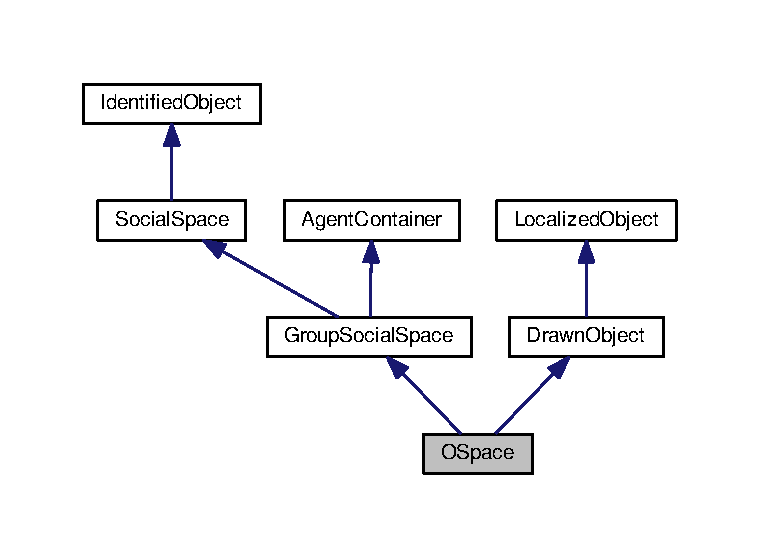
\includegraphics[width=350pt]{classOSpace__inherit__graph}
\end{center}
\end{figure}


Collaboration diagram for O\+Space\+:\nopagebreak
\begin{figure}[H]
\begin{center}
\leavevmode
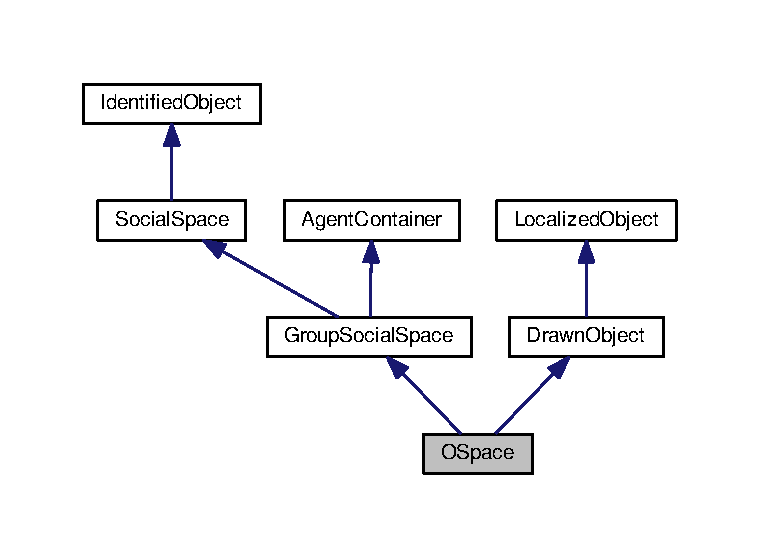
\includegraphics[width=350pt]{classOSpace__coll__graph}
\end{center}
\end{figure}
\subsection*{Public Member Functions}
\begin{DoxyCompactItemize}
\item 
\hyperlink{classOSpace_ae160e76b0b2d3c1367946f8bb965bd1e}{O\+Space} (int \hyperlink{classIdentifiedObject_ad044a317a9b573a3d1bcd025df166eb5}{id}=0)
\begin{DoxyCompactList}\small\item\em Constructor. \end{DoxyCompactList}\item 
\hyperlink{classOSpace_acd0c5685bc984af6287108710a1333ff}{O\+Space} (std\+::vector$<$ \hyperlink{classAgent}{Agent} $\ast$ $>$ \&agents, int \hyperlink{classIdentifiedObject_ad044a317a9b573a3d1bcd025df166eb5}{id}=0)
\begin{DoxyCompactList}\small\item\em Constructor. \end{DoxyCompactList}\item 
\hyperlink{classOSpace_af8078a93268b4064919701765ad59451}{$\sim$\+O\+Space} ()
\begin{DoxyCompactList}\small\item\em Destructor. \end{DoxyCompactList}\item 
void \hyperlink{classOSpace_a3d2cba9a025785ee12c0991085b08b21}{computeg\+Center} ()\hypertarget{classOSpace_a3d2cba9a025785ee12c0991085b08b21}{}\label{classOSpace_a3d2cba9a025785ee12c0991085b08b21}

\begin{DoxyCompactList}\small\item\em Compute the gravity center of the \hyperlink{classOSpace}{O\+Space} based on Agents positions. \end{DoxyCompactList}\item 
void \hyperlink{classOSpace_ad79a227974adf66884379213fbf54068}{sort\+Agents} ()\hypertarget{classOSpace_ad79a227974adf66884379213fbf54068}{}\label{classOSpace_ad79a227974adf66884379213fbf54068}

\begin{DoxyCompactList}\small\item\em Sort \hyperlink{classAgentContainer}{Agent\+Container} of the \hyperlink{classOSpace}{O\+Space} in clockwise order relative to gravity center. \end{DoxyCompactList}\item 
void \hyperlink{classOSpace_ad6163ea6ef19516251e397caf59fdf4d}{compute\+Centroids} ()\hypertarget{classOSpace_ad6163ea6ef19516251e397caf59fdf4d}{}\label{classOSpace_ad6163ea6ef19516251e397caf59fdf4d}

\begin{DoxyCompactList}\small\item\em Compute the centroids of each pair of \hyperlink{classAgent}{Agent} of the \hyperlink{classOSpace}{O\+Space} based on the field of view of every \hyperlink{classAgent}{Agent}. \end{DoxyCompactList}\item 
void \hyperlink{classOSpace_a2cc6d61b727df4a7e763a38f10183463}{compute\+Center} ()\hypertarget{classOSpace_a2cc6d61b727df4a7e763a38f10183463}{}\label{classOSpace_a2cc6d61b727df4a7e763a38f10183463}

\begin{DoxyCompactList}\small\item\em Compute the center of the \hyperlink{classFormation}{Formation} based on centroids. \end{DoxyCompactList}\item 
void \hyperlink{classOSpace_af73e9e5f18635010d63bf1cfcbc05f1c}{compute\+Covar\+Matrix} ()
\begin{DoxyCompactList}\small\item\em Compute the covariance matrix of the 2D gaussian mixture model. \end{DoxyCompactList}\item 
void \hyperlink{classOSpace_ac87ea026f6b4b6d00980e7f849e48e9b}{update} ()\hypertarget{classOSpace_ac87ea026f6b4b6d00980e7f849e48e9b}{}\label{classOSpace_ac87ea026f6b4b6d00980e7f849e48e9b}

\begin{DoxyCompactList}\small\item\em Update the \hyperlink{classOSpace}{O\+Space} by computing its gravity center, centroids and deduce the covariance matrix of the 2D gaussian mixture model. \end{DoxyCompactList}\item 
double \hyperlink{classOSpace_afa5d22b357c9639c7208c1cb5c6525fa}{phi} (Vector3d tested\+Point)
\begin{DoxyCompactList}\small\item\em Compute the value of the \hyperlink{classOSpace}{O\+Space} at a given point in space. \end{DoxyCompactList}\item 
bool \hyperlink{classOSpace_a96380f4ad674c9ecb29b345ff87d6b3f}{less} (Vector3d a, Vector3d b)
\begin{DoxyCompactList}\small\item\em Compare two vector based on the \hyperlink{classOSpace}{O\+Space} gravity center. \end{DoxyCompactList}\item 
Vector3d \hyperlink{classOSpace_ab9ddbaab88efeab63fb7e0e51de55036}{get\+Center} () const 
\begin{DoxyCompactList}\small\item\em Simple getter. \end{DoxyCompactList}\item 
void \hyperlink{classOSpace_aa495172e001ca1c6d5dd169f4cd4900b}{set\+Center} (const Vector3d \&\hyperlink{classOSpace_a7ec22529d88e51876ff7eba9cdcdca05}{center})
\begin{DoxyCompactList}\small\item\em Simpler setter. \end{DoxyCompactList}\item 
Vector3d \hyperlink{classOSpace_a45e9ea9c566d2fc13713a5092ce841f6}{getg\+Center} () const 
\begin{DoxyCompactList}\small\item\em Simple getter. \end{DoxyCompactList}\item 
void \hyperlink{classOSpace_aa4bbf797dfce6bd4414d33a57b346ea3}{setg\+Center} (const Vector3d \&\hyperlink{classOSpace_a023a293d79b949534f94eedbac932cec}{g\+Center})
\begin{DoxyCompactList}\small\item\em Simple setter. \end{DoxyCompactList}\end{DoxyCompactItemize}
\subsection*{Protected Attributes}
\begin{DoxyCompactItemize}
\item 
std\+::vector$<$ std\+::vector$<$ Vector3d $>$ $>$ \hyperlink{classOSpace_ada0f8c061d4b2623077c7524a540bb4d}{dh\+\_\+seg}\hypertarget{classOSpace_ada0f8c061d4b2623077c7524a540bb4d}{}\label{classOSpace_ada0f8c061d4b2623077c7524a540bb4d}

\begin{DoxyCompactList}\small\item\em List of DH vector representing the interpersonnal distance between the Agents. \end{DoxyCompactList}\item 
std\+::vector$<$ std\+::vector$<$ Vector3d $>$ $>$ \hyperlink{classOSpace_a6a5fdc339135907855b6a9bc2f69fca7}{di\+\_\+seg}\hypertarget{classOSpace_a6a5fdc339135907855b6a9bc2f69fca7}{}\label{classOSpace_a6a5fdc339135907855b6a9bc2f69fca7}

\begin{DoxyCompactList}\small\item\em List of DI vector representing the distance between field of view intersection of Agents. \end{DoxyCompactList}\item 
Vector3d \hyperlink{classOSpace_a7ec22529d88e51876ff7eba9cdcdca05}{center}\hypertarget{classOSpace_a7ec22529d88e51876ff7eba9cdcdca05}{}\label{classOSpace_a7ec22529d88e51876ff7eba9cdcdca05}

\begin{DoxyCompactList}\small\item\em The center of the \hyperlink{classOSpace}{O\+Space}. \end{DoxyCompactList}\item 
Vector3d \hyperlink{classOSpace_a023a293d79b949534f94eedbac932cec}{g\+Center}\hypertarget{classOSpace_a023a293d79b949534f94eedbac932cec}{}\label{classOSpace_a023a293d79b949534f94eedbac932cec}

\begin{DoxyCompactList}\small\item\em The gravity center based on the Agents position. \end{DoxyCompactList}\item 
double \hyperlink{classOSpace_a0c7df223dae1d6cf274ce9271dfafe8c}{rotation} = 0.\+0f\hypertarget{classOSpace_a0c7df223dae1d6cf274ce9271dfafe8c}{}\label{classOSpace_a0c7df223dae1d6cf274ce9271dfafe8c}

\begin{DoxyCompactList}\small\item\em The rotation applied to the 2D gaussian mixture model. \end{DoxyCompactList}\item 
std\+::vector$<$ Vector3d $>$ \hyperlink{classOSpace_acc818308e36fff24106eaa8f00388038}{intersection\+Points}\hypertarget{classOSpace_acc818308e36fff24106eaa8f00388038}{}\label{classOSpace_acc818308e36fff24106eaa8f00388038}

\begin{DoxyCompactList}\small\item\em List of field of view intersection point between Agents. \end{DoxyCompactList}\item 
std\+::vector$<$ Vector3d $>$ \hyperlink{classOSpace_aaa01a3a29082df6be390aa1869946af7}{centroids}\hypertarget{classOSpace_aaa01a3a29082df6be390aa1869946af7}{}\label{classOSpace_aaa01a3a29082df6be390aa1869946af7}

\begin{DoxyCompactList}\small\item\em List of the centroid points based on intersection points and Agents position. \end{DoxyCompactList}\item 
Matrix$<$ double, 2, 2 $>$ \hyperlink{classOSpace_af7b7e14739162e0b40da89484c351dd7}{covar\+Matrix}\hypertarget{classOSpace_af7b7e14739162e0b40da89484c351dd7}{}\label{classOSpace_af7b7e14739162e0b40da89484c351dd7}

\begin{DoxyCompactList}\small\item\em The covariance matrix of the 2D gaussian mixture model. \end{DoxyCompactList}\end{DoxyCompactItemize}


\subsection{Detailed Description}
This class is an implementation of the \hyperlink{classGroupSocialSpace}{Group\+Social\+Space}. 

This class is an implementation of the \hyperlink{classGroupSocialSpace}{Group\+Social\+Space} represented by a 2D gaussian mixture model based on interpersonal distances and a algorithm to find the center of the related \hyperlink{classFormation}{Formation}. 

\subsection{Constructor \& Destructor Documentation}
\index{O\+Space@{O\+Space}!O\+Space@{O\+Space}}
\index{O\+Space@{O\+Space}!O\+Space@{O\+Space}}
\subsubsection[{\texorpdfstring{O\+Space(int id=0)}{OSpace(int id=0)}}]{\setlength{\rightskip}{0pt plus 5cm}O\+Space\+::\+O\+Space (
\begin{DoxyParamCaption}
\item[{int}]{id = {\ttfamily 0}}
\end{DoxyParamCaption}
)}\hypertarget{classOSpace_ae160e76b0b2d3c1367946f8bb965bd1e}{}\label{classOSpace_ae160e76b0b2d3c1367946f8bb965bd1e}


Constructor. 

Constructor of the \hyperlink{classOSpace}{O\+Space} class, with no \hyperlink{classAgent}{Agent}


\begin{DoxyParams}{Parameters}
{\em id} & \+: The unique identifier of the \hyperlink{classOSpace}{O\+Space} \\
\hline
\end{DoxyParams}
\index{O\+Space@{O\+Space}!O\+Space@{O\+Space}}
\index{O\+Space@{O\+Space}!O\+Space@{O\+Space}}
\subsubsection[{\texorpdfstring{O\+Space(std\+::vector$<$ Agent $\ast$ $>$ \&agents, int id=0)}{OSpace(std::vector< Agent * > &agents, int id=0)}}]{\setlength{\rightskip}{0pt plus 5cm}O\+Space\+::\+O\+Space (
\begin{DoxyParamCaption}
\item[{std\+::vector$<$ {\bf Agent} $\ast$ $>$ \&}]{agents, }
\item[{int}]{id = {\ttfamily 0}}
\end{DoxyParamCaption}
)}\hypertarget{classOSpace_acd0c5685bc984af6287108710a1333ff}{}\label{classOSpace_acd0c5685bc984af6287108710a1333ff}


Constructor. 

Constructor of the \hyperlink{classOSpace}{O\+Space} class, for the Agents in parameter


\begin{DoxyParams}{Parameters}
{\em agents} & \+: The Agents related to the \hyperlink{classGroupSocialSpace}{Group\+Social\+Space} \\
\hline
{\em id} & \+: The unique identifier of the \hyperlink{classGroupSocialSpace}{Group\+Social\+Space} \\
\hline
\end{DoxyParams}
\index{O\+Space@{O\+Space}!````~O\+Space@{$\sim$\+O\+Space}}
\index{````~O\+Space@{$\sim$\+O\+Space}!O\+Space@{O\+Space}}
\subsubsection[{\texorpdfstring{$\sim$\+O\+Space()}{~OSpace()}}]{\setlength{\rightskip}{0pt plus 5cm}O\+Space\+::$\sim$\+O\+Space (
\begin{DoxyParamCaption}
{}
\end{DoxyParamCaption}
)}\hypertarget{classOSpace_af8078a93268b4064919701765ad59451}{}\label{classOSpace_af8078a93268b4064919701765ad59451}


Destructor. 

Destructor of the \hyperlink{classOSpace}{O\+Space} class 

\subsection{Member Function Documentation}
\index{O\+Space@{O\+Space}!compute\+Covar\+Matrix@{compute\+Covar\+Matrix}}
\index{compute\+Covar\+Matrix@{compute\+Covar\+Matrix}!O\+Space@{O\+Space}}
\subsubsection[{\texorpdfstring{compute\+Covar\+Matrix()}{computeCovarMatrix()}}]{\setlength{\rightskip}{0pt plus 5cm}void O\+Space\+::compute\+Covar\+Matrix (
\begin{DoxyParamCaption}
{}
\end{DoxyParamCaption}
)}\hypertarget{classOSpace_af73e9e5f18635010d63bf1cfcbc05f1c}{}\label{classOSpace_af73e9e5f18635010d63bf1cfcbc05f1c}


Compute the covariance matrix of the 2D gaussian mixture model. 

Compute the covariance matrix of the 2D gaussian mixture model based on interpersonnal distance between Agents \index{O\+Space@{O\+Space}!get\+Center@{get\+Center}}
\index{get\+Center@{get\+Center}!O\+Space@{O\+Space}}
\subsubsection[{\texorpdfstring{get\+Center() const }{getCenter() const }}]{\setlength{\rightskip}{0pt plus 5cm}Vector3d O\+Space\+::get\+Center (
\begin{DoxyParamCaption}
{}
\end{DoxyParamCaption}
) const}\hypertarget{classOSpace_ab9ddbaab88efeab63fb7e0e51de55036}{}\label{classOSpace_ab9ddbaab88efeab63fb7e0e51de55036}


Simple getter. 

\begin{DoxyReturn}{Returns}
center 
\end{DoxyReturn}
\index{O\+Space@{O\+Space}!getg\+Center@{getg\+Center}}
\index{getg\+Center@{getg\+Center}!O\+Space@{O\+Space}}
\subsubsection[{\texorpdfstring{getg\+Center() const }{getgCenter() const }}]{\setlength{\rightskip}{0pt plus 5cm}Vector3d O\+Space\+::getg\+Center (
\begin{DoxyParamCaption}
{}
\end{DoxyParamCaption}
) const}\hypertarget{classOSpace_a45e9ea9c566d2fc13713a5092ce841f6}{}\label{classOSpace_a45e9ea9c566d2fc13713a5092ce841f6}


Simple getter. 

\begin{DoxyReturn}{Returns}
g\+Center 
\end{DoxyReturn}
\index{O\+Space@{O\+Space}!less@{less}}
\index{less@{less}!O\+Space@{O\+Space}}
\subsubsection[{\texorpdfstring{less(\+Vector3d a, Vector3d b)}{less(Vector3d a, Vector3d b)}}]{\setlength{\rightskip}{0pt plus 5cm}bool O\+Space\+::less (
\begin{DoxyParamCaption}
\item[{Vector3d}]{a, }
\item[{Vector3d}]{b}
\end{DoxyParamCaption}
)}\hypertarget{classOSpace_a96380f4ad674c9ecb29b345ff87d6b3f}{}\label{classOSpace_a96380f4ad674c9ecb29b345ff87d6b3f}


Compare two vector based on the \hyperlink{classOSpace}{O\+Space} gravity center. 

Compare two vector based on the \hyperlink{classOSpace}{O\+Space} gravity center to order them clockwise


\begin{DoxyParams}{Parameters}
{\em a} & \+: The first \hyperlink{classAgent}{Agent} position \\
\hline
{\em b} & \+: The second \hyperlink{classAgent}{Agent} position \\
\hline
\end{DoxyParams}
\begin{DoxyReturn}{Returns}
1 if a \hyperlink{classAgent}{Agent} is before b \hyperlink{classAgent}{Agent} in clockwise order relative to g\+Center, 0 otherwise 
\end{DoxyReturn}
\index{O\+Space@{O\+Space}!phi@{phi}}
\index{phi@{phi}!O\+Space@{O\+Space}}
\subsubsection[{\texorpdfstring{phi(\+Vector3d tested\+Point)}{phi(Vector3d testedPoint)}}]{\setlength{\rightskip}{0pt plus 5cm}double O\+Space\+::phi (
\begin{DoxyParamCaption}
\item[{Vector3d}]{tested\+Point}
\end{DoxyParamCaption}
)}\hypertarget{classOSpace_afa5d22b357c9639c7208c1cb5c6525fa}{}\label{classOSpace_afa5d22b357c9639c7208c1cb5c6525fa}


Compute the value of the \hyperlink{classOSpace}{O\+Space} at a given point in space. 


\begin{DoxyParams}{Parameters}
{\em tested\+Point} & \+: The coordinates of the point in the real frame coordinates \hyperlink{classWorld}{World}\\
\hline
\end{DoxyParams}
\begin{DoxyReturn}{Returns}
The value of the \hyperlink{classOSpace}{O\+Space} at the given point 
\end{DoxyReturn}
\index{O\+Space@{O\+Space}!set\+Center@{set\+Center}}
\index{set\+Center@{set\+Center}!O\+Space@{O\+Space}}
\subsubsection[{\texorpdfstring{set\+Center(const Vector3d \&center)}{setCenter(const Vector3d &center)}}]{\setlength{\rightskip}{0pt plus 5cm}void O\+Space\+::set\+Center (
\begin{DoxyParamCaption}
\item[{const Vector3d \&}]{center}
\end{DoxyParamCaption}
)}\hypertarget{classOSpace_aa495172e001ca1c6d5dd169f4cd4900b}{}\label{classOSpace_aa495172e001ca1c6d5dd169f4cd4900b}


Simpler setter. 


\begin{DoxyParams}{Parameters}
{\em center} & \\
\hline
\end{DoxyParams}
\index{O\+Space@{O\+Space}!setg\+Center@{setg\+Center}}
\index{setg\+Center@{setg\+Center}!O\+Space@{O\+Space}}
\subsubsection[{\texorpdfstring{setg\+Center(const Vector3d \&g\+Center)}{setgCenter(const Vector3d &gCenter)}}]{\setlength{\rightskip}{0pt plus 5cm}void O\+Space\+::setg\+Center (
\begin{DoxyParamCaption}
\item[{const Vector3d \&}]{g\+Center}
\end{DoxyParamCaption}
)}\hypertarget{classOSpace_aa4bbf797dfce6bd4414d33a57b346ea3}{}\label{classOSpace_aa4bbf797dfce6bd4414d33a57b346ea3}


Simple setter. 


\begin{DoxyParams}{Parameters}
{\em g\+Center} & \\
\hline
\end{DoxyParams}


The documentation for this class was generated from the following files\+:\begin{DoxyCompactItemize}
\item 
src/social\+Space/\hyperlink{OSpace_8h}{O\+Space.\+h}\item 
src/social\+Space/\hyperlink{OSpace_8cpp}{O\+Space.\+cpp}\end{DoxyCompactItemize}

\hypertarget{classPersonnalSocialSpace}{}\section{Personnal\+Social\+Space Class Reference}
\label{classPersonnalSocialSpace}\index{Personnal\+Social\+Space@{Personnal\+Social\+Space}}


This class is an interface to implement representation of a \hyperlink{classPersonnalSocialSpace}{Personnal\+Social\+Space}.  




{\ttfamily \#include $<$Personnal\+Social\+Space.\+h$>$}



Inheritance diagram for Personnal\+Social\+Space\+:\nopagebreak
\begin{figure}[H]
\begin{center}
\leavevmode
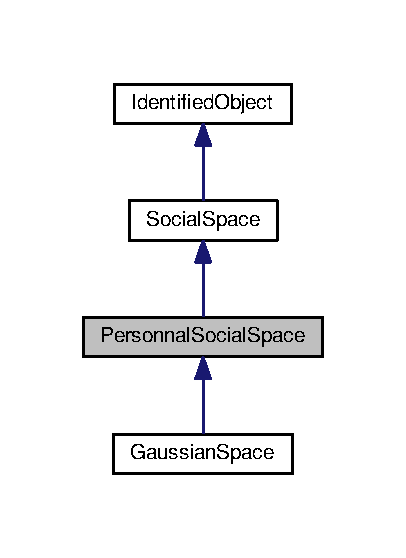
\includegraphics[width=195pt]{classPersonnalSocialSpace__inherit__graph}
\end{center}
\end{figure}


Collaboration diagram for Personnal\+Social\+Space\+:\nopagebreak
\begin{figure}[H]
\begin{center}
\leavevmode
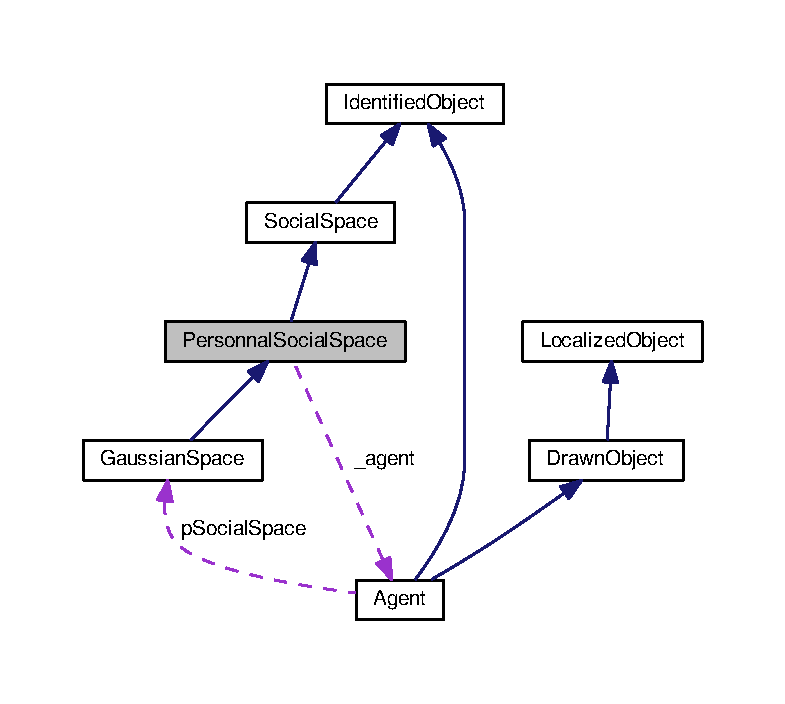
\includegraphics[width=350pt]{classPersonnalSocialSpace__coll__graph}
\end{center}
\end{figure}
\subsection*{Public Member Functions}
\begin{DoxyCompactItemize}
\item 
\hyperlink{classPersonnalSocialSpace_a7a1179eca56db918a2d7bd48b91fe23e}{Personnal\+Social\+Space} (\hyperlink{classAgent}{Agent} $\ast$agent, int \hyperlink{classIdentifiedObject_ad044a317a9b573a3d1bcd025df166eb5}{id}=0)
\begin{DoxyCompactList}\small\item\em Constructor. \end{DoxyCompactList}\item 
virtual \hyperlink{classPersonnalSocialSpace_aa4df470b07dddfcca155a47cf8dc8739}{$\sim$\+Personnal\+Social\+Space} ()
\begin{DoxyCompactList}\small\item\em Destructor. \end{DoxyCompactList}\end{DoxyCompactItemize}
\subsection*{Protected Attributes}
\begin{DoxyCompactItemize}
\item 
\hyperlink{classAgent}{Agent} $\ast$ \hyperlink{classPersonnalSocialSpace_a73735af1f47bfdc90ea6d7f244aa10d4}{\+\_\+agent}\hypertarget{classPersonnalSocialSpace_a73735af1f47bfdc90ea6d7f244aa10d4}{}\label{classPersonnalSocialSpace_a73735af1f47bfdc90ea6d7f244aa10d4}

\begin{DoxyCompactList}\small\item\em The \hyperlink{classAgent}{Agent} related to the \hyperlink{classPersonnalSocialSpace}{Personnal\+Social\+Space}. \end{DoxyCompactList}\end{DoxyCompactItemize}


\subsection{Detailed Description}
This class is an interface to implement representation of a \hyperlink{classPersonnalSocialSpace}{Personnal\+Social\+Space}. 

This class is an interface to implement representation of the \hyperlink{classPersonnalSocialSpace}{Personnal\+Social\+Space} of an \hyperlink{classAgent}{Agent} 

\subsection{Constructor \& Destructor Documentation}
\index{Personnal\+Social\+Space@{Personnal\+Social\+Space}!Personnal\+Social\+Space@{Personnal\+Social\+Space}}
\index{Personnal\+Social\+Space@{Personnal\+Social\+Space}!Personnal\+Social\+Space@{Personnal\+Social\+Space}}
\subsubsection[{\texorpdfstring{Personnal\+Social\+Space(\+Agent $\ast$agent, int id=0)}{PersonnalSocialSpace(Agent *agent, int id=0)}}]{\setlength{\rightskip}{0pt plus 5cm}Personnal\+Social\+Space\+::\+Personnal\+Social\+Space (
\begin{DoxyParamCaption}
\item[{{\bf Agent} $\ast$}]{agent, }
\item[{int}]{id = {\ttfamily 0}}
\end{DoxyParamCaption}
)}\hypertarget{classPersonnalSocialSpace_a7a1179eca56db918a2d7bd48b91fe23e}{}\label{classPersonnalSocialSpace_a7a1179eca56db918a2d7bd48b91fe23e}


Constructor. 

Constructor of the \hyperlink{classPersonnalSocialSpace}{Personnal\+Social\+Space} class


\begin{DoxyParams}{Parameters}
{\em agent} & \+: The \hyperlink{classAgent}{Agent} related to the \hyperlink{classPersonnalSocialSpace}{Personnal\+Social\+Space} \\
\hline
{\em id} & \+: The unique identifier of the \hyperlink{classSocialSpace}{Social\+Space} \\
\hline
\end{DoxyParams}
\index{Personnal\+Social\+Space@{Personnal\+Social\+Space}!````~Personnal\+Social\+Space@{$\sim$\+Personnal\+Social\+Space}}
\index{````~Personnal\+Social\+Space@{$\sim$\+Personnal\+Social\+Space}!Personnal\+Social\+Space@{Personnal\+Social\+Space}}
\subsubsection[{\texorpdfstring{$\sim$\+Personnal\+Social\+Space()}{~PersonnalSocialSpace()}}]{\setlength{\rightskip}{0pt plus 5cm}Personnal\+Social\+Space\+::$\sim$\+Personnal\+Social\+Space (
\begin{DoxyParamCaption}
{}
\end{DoxyParamCaption}
)\hspace{0.3cm}{\ttfamily [virtual]}}\hypertarget{classPersonnalSocialSpace_aa4df470b07dddfcca155a47cf8dc8739}{}\label{classPersonnalSocialSpace_aa4df470b07dddfcca155a47cf8dc8739}


Destructor. 

Destructor of the \hyperlink{classPersonnalSocialSpace}{Personnal\+Social\+Space} class 

The documentation for this class was generated from the following files\+:\begin{DoxyCompactItemize}
\item 
src/social\+Space/\hyperlink{PersonnalSocialSpace_8h}{Personnal\+Social\+Space.\+h}\item 
src/social\+Space/\hyperlink{PersonnalSocialSpace_8cpp}{Personnal\+Social\+Space.\+cpp}\end{DoxyCompactItemize}

\hypertarget{classPopulation}{}\section{Population Class Reference}
\label{classPopulation}\index{Population@{Population}}


This class represent \hyperlink{classPopulation}{Population} around the \hyperlink{classRobot}{Robot}.  




{\ttfamily \#include $<$Population.\+h$>$}



Inheritance diagram for Population\+:\nopagebreak
\begin{figure}[H]
\begin{center}
\leavevmode
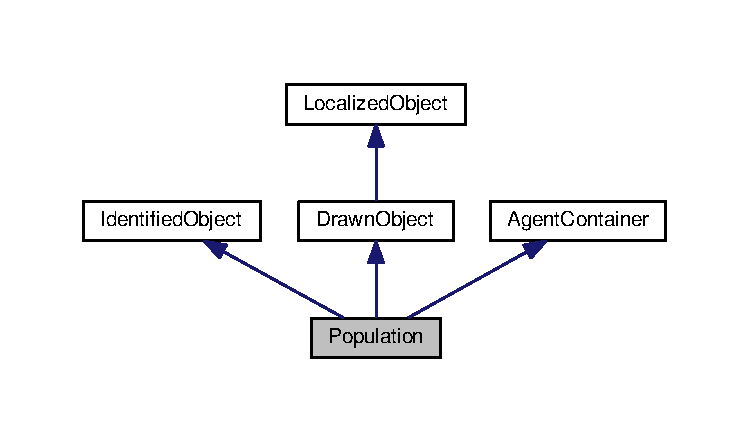
\includegraphics[width=350pt]{classPopulation__inherit__graph}
\end{center}
\end{figure}


Collaboration diagram for Population\+:\nopagebreak
\begin{figure}[H]
\begin{center}
\leavevmode
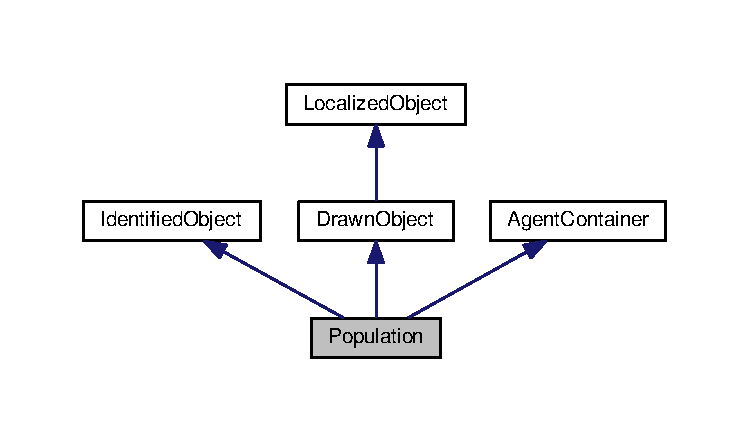
\includegraphics[width=350pt]{classPopulation__coll__graph}
\end{center}
\end{figure}
\subsection*{Public Member Functions}
\begin{DoxyCompactItemize}
\item 
\hyperlink{classPopulation_a013e3f3d1a26f4ff64570ea91ae9cb22}{Population} (std\+::vector$<$ \hyperlink{classAgent}{Agent} $\ast$ $>$ agents, Vector3d \hyperlink{classLocalizedObject_a340834deefc9e5c39da1f26c4ebf4f8c}{position}=Vector3d(), int \hyperlink{classIdentifiedObject_ad044a317a9b573a3d1bcd025df166eb5}{id}=0)
\begin{DoxyCompactList}\small\item\em Constructor. \end{DoxyCompactList}\item 
\hyperlink{classPopulation_a3284afe8c0a8c10d7ce7a57c52f2f046}{Population} (Vector3d \hyperlink{classLocalizedObject_a340834deefc9e5c39da1f26c4ebf4f8c}{position}=Vector3d(), int \hyperlink{classIdentifiedObject_ad044a317a9b573a3d1bcd025df166eb5}{id}=0)
\begin{DoxyCompactList}\small\item\em Constructor. \end{DoxyCompactList}\item 
\hyperlink{classPopulation_a4c8cedd0f038e41746fb6084639f5616}{$\sim$\+Population} ()
\begin{DoxyCompactList}\small\item\em Destructor. \end{DoxyCompactList}\item 
\hyperlink{classFormation}{Formation} $\ast$ \hyperlink{classPopulation_aa39ee4e80d5cfd38a946395be1c49177}{get\+Highest\+Formation\+Interaction\+Potential} ()
\begin{DoxyCompactList}\small\item\em Find the \hyperlink{classFormation}{Formation} with the highest interaction potential. \end{DoxyCompactList}\item 
\hyperlink{classFormation}{Formation} $\ast$ \hyperlink{classPopulation_ad13aa87e5d1088faeca0071f8e3637d0}{get\+Related\+Formation} (unsigned int agent\+Id)
\begin{DoxyCompactList}\small\item\em Find the \hyperlink{classFormation}{Formation} related to the \hyperlink{classAgent}{Agent}. \end{DoxyCompactList}\item 
\hyperlink{classFormation}{Formation} $\ast$ \hyperlink{classPopulation_a3ebbdff664c498dcdbcdf9941c710b6f}{get\+Related\+Formation} (\hyperlink{classAgent}{Agent} $\ast$a)
\begin{DoxyCompactList}\small\item\em Find the \hyperlink{classFormation}{Formation} related to the \hyperlink{classAgent}{Agent} Alias to get\+Related\+Formation function by \hyperlink{classAgent}{Agent} id. \end{DoxyCompactList}\item 
void \hyperlink{classPopulation_a5a42d2a59c007194fec4d3168807e54d}{clear} ()
\begin{DoxyCompactList}\small\item\em Clear the \hyperlink{classPopulation}{Population}. \end{DoxyCompactList}\item 
int \hyperlink{classPopulation_a8d552e2753c24f694066f80a62374b7e}{is\+Grouped} (\hyperlink{classAgent}{Agent} $\ast$agent)
\begin{DoxyCompactList}\small\item\em Check if the \hyperlink{classAgent}{Agent} is part of a \hyperlink{classFormation}{Formation} Alias to is\+Grouped function by \hyperlink{classAgent}{Agent} id. \end{DoxyCompactList}\item 
int \hyperlink{classPopulation_a708335a33351906ecf7861c1bbcffa46}{is\+Grouped} (unsigned int agent\+Id)
\begin{DoxyCompactList}\small\item\em Check if the \hyperlink{classAgent}{Agent} is part of a \hyperlink{classFormation}{Formation}. \end{DoxyCompactList}\item 
void \hyperlink{classPopulation_a2cb08ce6189854de61a8395242854050}{push\+Formation} (\hyperlink{classFormation}{Formation} $\ast$formation)
\begin{DoxyCompactList}\small\item\em Add a \hyperlink{classFormation}{Formation} to the \hyperlink{classPopulation}{Population}. \end{DoxyCompactList}\item 
int \hyperlink{classPopulation_a576b1d3fd6fdfce01d3c320dca09d736}{remove\+Formation} (unsigned int formation\+Id)
\begin{DoxyCompactList}\small\item\em Remove a \hyperlink{classFormation}{Formation} by id from the \hyperlink{classPopulation}{Population} and the corresponding \hyperlink{classGroupSocialSpace}{Group\+Social\+Space}. \end{DoxyCompactList}\item 
void \hyperlink{classPopulation_a48a1ed3703002aaf17fcd70e08a36567}{clear\+Formations} ()
\begin{DoxyCompactList}\small\item\em Clear the \hyperlink{classFormation}{Formation} list. \end{DoxyCompactList}\item 
const std\+::vector$<$ \hyperlink{classFormation}{Formation} $\ast$ $>$ \& \hyperlink{classPopulation_aaca5634d7b5cc94d2268812e492e3c13}{get\+Formations} () const 
\begin{DoxyCompactList}\small\item\em Simple getter. \end{DoxyCompactList}\item 
void \hyperlink{classPopulation_aa14826487ffb94ee077869950bf04465}{set\+Formations} (const std\+::vector$<$ \hyperlink{classFormation}{Formation} $\ast$ $>$ \&formations)
\begin{DoxyCompactList}\small\item\em Simpler setter. \end{DoxyCompactList}\end{DoxyCompactItemize}
\subsection*{Additional Inherited Members}


\subsection{Detailed Description}
This class represent \hyperlink{classPopulation}{Population} around the \hyperlink{classRobot}{Robot}. 

This class represent \hyperlink{classPopulation}{Population} around the \hyperlink{classRobot}{Robot}, it contains all the Agents with the Formations detected in this \hyperlink{classPopulation}{Population}. 

\subsection{Constructor \& Destructor Documentation}
\index{Population@{Population}!Population@{Population}}
\index{Population@{Population}!Population@{Population}}
\subsubsection[{\texorpdfstring{Population(std\+::vector$<$ Agent $\ast$ $>$ agents, Vector3d position=\+Vector3d(), int id=0)}{Population(std::vector< Agent * > agents, Vector3d position=Vector3d(), int id=0)}}]{\setlength{\rightskip}{0pt plus 5cm}Population\+::\+Population (
\begin{DoxyParamCaption}
\item[{std\+::vector$<$ {\bf Agent} $\ast$ $>$}]{agents, }
\item[{Vector3d}]{position = {\ttfamily Vector3d()}, }
\item[{int}]{id = {\ttfamily 0}}
\end{DoxyParamCaption}
)}\hypertarget{classPopulation_a013e3f3d1a26f4ff64570ea91ae9cb22}{}\label{classPopulation_a013e3f3d1a26f4ff64570ea91ae9cb22}


Constructor. 

Constructor of the \hyperlink{classPopulation}{Population} class


\begin{DoxyParams}{Parameters}
{\em agents} & \+: List of initial Agents that are part of the \hyperlink{classPopulation}{Population} \\
\hline
{\em position} & \+: Position of the \hyperlink{classPopulation}{Population} (required by \hyperlink{classDrawnObject}{Drawn\+Object} but useless here) \\
\hline
{\em id} & \+: Unique identifier of the \hyperlink{classPopulation}{Population} \\
\hline
\end{DoxyParams}
\index{Population@{Population}!Population@{Population}}
\index{Population@{Population}!Population@{Population}}
\subsubsection[{\texorpdfstring{Population(\+Vector3d position=\+Vector3d(), int id=0)}{Population(Vector3d position=Vector3d(), int id=0)}}]{\setlength{\rightskip}{0pt plus 5cm}Population\+::\+Population (
\begin{DoxyParamCaption}
\item[{Vector3d}]{position = {\ttfamily Vector3d()}, }
\item[{int}]{id = {\ttfamily 0}}
\end{DoxyParamCaption}
)}\hypertarget{classPopulation_a3284afe8c0a8c10d7ce7a57c52f2f046}{}\label{classPopulation_a3284afe8c0a8c10d7ce7a57c52f2f046}


Constructor. 

Constructor of the \hyperlink{classPopulation}{Population} class


\begin{DoxyParams}{Parameters}
{\em position} & \+: Position of the \hyperlink{classPopulation}{Population} (required by \hyperlink{classDrawnObject}{Drawn\+Object} but useless here) \\
\hline
{\em id} & \+: Unique identifier of the \hyperlink{classPopulation}{Population} \\
\hline
\end{DoxyParams}
\index{Population@{Population}!````~Population@{$\sim$\+Population}}
\index{````~Population@{$\sim$\+Population}!Population@{Population}}
\subsubsection[{\texorpdfstring{$\sim$\+Population()}{~Population()}}]{\setlength{\rightskip}{0pt plus 5cm}Population\+::$\sim$\+Population (
\begin{DoxyParamCaption}
{}
\end{DoxyParamCaption}
)}\hypertarget{classPopulation_a4c8cedd0f038e41746fb6084639f5616}{}\label{classPopulation_a4c8cedd0f038e41746fb6084639f5616}


Destructor. 

Destructor of the \hyperlink{classPopulation}{Population} class, destroy every Agents and Formations related to this \hyperlink{classPopulation}{Population} 

\subsection{Member Function Documentation}
\index{Population@{Population}!clear@{clear}}
\index{clear@{clear}!Population@{Population}}
\subsubsection[{\texorpdfstring{clear()}{clear()}}]{\setlength{\rightskip}{0pt plus 5cm}void Population\+::clear (
\begin{DoxyParamCaption}
{}
\end{DoxyParamCaption}
)}\hypertarget{classPopulation_a5a42d2a59c007194fec4d3168807e54d}{}\label{classPopulation_a5a42d2a59c007194fec4d3168807e54d}


Clear the \hyperlink{classPopulation}{Population}. 

Destroy all Agents and Formations \index{Population@{Population}!clear\+Formations@{clear\+Formations}}
\index{clear\+Formations@{clear\+Formations}!Population@{Population}}
\subsubsection[{\texorpdfstring{clear\+Formations()}{clearFormations()}}]{\setlength{\rightskip}{0pt plus 5cm}void Population\+::clear\+Formations (
\begin{DoxyParamCaption}
{}
\end{DoxyParamCaption}
)}\hypertarget{classPopulation_a48a1ed3703002aaf17fcd70e08a36567}{}\label{classPopulation_a48a1ed3703002aaf17fcd70e08a36567}


Clear the \hyperlink{classFormation}{Formation} list. 

This function do not call the \hyperlink{classFormation}{Formation} destructor \index{Population@{Population}!get\+Formations@{get\+Formations}}
\index{get\+Formations@{get\+Formations}!Population@{Population}}
\subsubsection[{\texorpdfstring{get\+Formations() const }{getFormations() const }}]{\setlength{\rightskip}{0pt plus 5cm}const std\+::vector$<$ {\bf Formation} $\ast$ $>$ \& Population\+::get\+Formations (
\begin{DoxyParamCaption}
{}
\end{DoxyParamCaption}
) const}\hypertarget{classPopulation_aaca5634d7b5cc94d2268812e492e3c13}{}\label{classPopulation_aaca5634d7b5cc94d2268812e492e3c13}


Simple getter. 

\begin{DoxyReturn}{Returns}
Formations 
\end{DoxyReturn}
\index{Population@{Population}!get\+Highest\+Formation\+Interaction\+Potential@{get\+Highest\+Formation\+Interaction\+Potential}}
\index{get\+Highest\+Formation\+Interaction\+Potential@{get\+Highest\+Formation\+Interaction\+Potential}!Population@{Population}}
\subsubsection[{\texorpdfstring{get\+Highest\+Formation\+Interaction\+Potential()}{getHighestFormationInteractionPotential()}}]{\setlength{\rightskip}{0pt plus 5cm}{\bf Formation}$\ast$ Population\+::get\+Highest\+Formation\+Interaction\+Potential (
\begin{DoxyParamCaption}
{}
\end{DoxyParamCaption}
)}\hypertarget{classPopulation_aa39ee4e80d5cfd38a946395be1c49177}{}\label{classPopulation_aa39ee4e80d5cfd38a946395be1c49177}


Find the \hyperlink{classFormation}{Formation} with the highest interaction potential. 

\begin{DoxyReturn}{Returns}
The \hyperlink{classFormation}{Formation} with the highest interaction potential in the \hyperlink{classPopulation}{Population} 
\end{DoxyReturn}
\index{Population@{Population}!get\+Related\+Formation@{get\+Related\+Formation}}
\index{get\+Related\+Formation@{get\+Related\+Formation}!Population@{Population}}
\subsubsection[{\texorpdfstring{get\+Related\+Formation(unsigned int agent\+Id)}{getRelatedFormation(unsigned int agentId)}}]{\setlength{\rightskip}{0pt plus 5cm}{\bf Formation} $\ast$ Population\+::get\+Related\+Formation (
\begin{DoxyParamCaption}
\item[{unsigned int}]{agent\+Id}
\end{DoxyParamCaption}
)}\hypertarget{classPopulation_ad13aa87e5d1088faeca0071f8e3637d0}{}\label{classPopulation_ad13aa87e5d1088faeca0071f8e3637d0}


Find the \hyperlink{classFormation}{Formation} related to the \hyperlink{classAgent}{Agent}. 

\begin{DoxyReturn}{Returns}
The \hyperlink{classFormation}{Formation} in which the \hyperlink{classAgent}{Agent} is taking part 
\end{DoxyReturn}
\index{Population@{Population}!get\+Related\+Formation@{get\+Related\+Formation}}
\index{get\+Related\+Formation@{get\+Related\+Formation}!Population@{Population}}
\subsubsection[{\texorpdfstring{get\+Related\+Formation(\+Agent $\ast$a)}{getRelatedFormation(Agent *a)}}]{\setlength{\rightskip}{0pt plus 5cm}{\bf Formation} $\ast$ Population\+::get\+Related\+Formation (
\begin{DoxyParamCaption}
\item[{{\bf Agent} $\ast$}]{a}
\end{DoxyParamCaption}
)}\hypertarget{classPopulation_a3ebbdff664c498dcdbcdf9941c710b6f}{}\label{classPopulation_a3ebbdff664c498dcdbcdf9941c710b6f}


Find the \hyperlink{classFormation}{Formation} related to the \hyperlink{classAgent}{Agent} Alias to get\+Related\+Formation function by \hyperlink{classAgent}{Agent} id. 

\begin{DoxyReturn}{Returns}
The \hyperlink{classFormation}{Formation} in which the \hyperlink{classAgent}{Agent} is taking part 
\end{DoxyReturn}
\index{Population@{Population}!is\+Grouped@{is\+Grouped}}
\index{is\+Grouped@{is\+Grouped}!Population@{Population}}
\subsubsection[{\texorpdfstring{is\+Grouped(\+Agent $\ast$agent)}{isGrouped(Agent *agent)}}]{\setlength{\rightskip}{0pt plus 5cm}int Population\+::is\+Grouped (
\begin{DoxyParamCaption}
\item[{{\bf Agent} $\ast$}]{agent}
\end{DoxyParamCaption}
)}\hypertarget{classPopulation_a8d552e2753c24f694066f80a62374b7e}{}\label{classPopulation_a8d552e2753c24f694066f80a62374b7e}


Check if the \hyperlink{classAgent}{Agent} is part of a \hyperlink{classFormation}{Formation} Alias to is\+Grouped function by \hyperlink{classAgent}{Agent} id. 


\begin{DoxyParams}{Parameters}
{\em agent} & \+: The \hyperlink{classAgent}{Agent} to check \\
\hline
\end{DoxyParams}
\begin{DoxyReturn}{Returns}
1 if \hyperlink{classAgent}{Agent} is in a \hyperlink{classFormation}{Formation}, 0 otherwise 
\end{DoxyReturn}
\index{Population@{Population}!is\+Grouped@{is\+Grouped}}
\index{is\+Grouped@{is\+Grouped}!Population@{Population}}
\subsubsection[{\texorpdfstring{is\+Grouped(unsigned int agent\+Id)}{isGrouped(unsigned int agentId)}}]{\setlength{\rightskip}{0pt plus 5cm}int Population\+::is\+Grouped (
\begin{DoxyParamCaption}
\item[{unsigned int}]{agent\+Id}
\end{DoxyParamCaption}
)}\hypertarget{classPopulation_a708335a33351906ecf7861c1bbcffa46}{}\label{classPopulation_a708335a33351906ecf7861c1bbcffa46}


Check if the \hyperlink{classAgent}{Agent} is part of a \hyperlink{classFormation}{Formation}. 


\begin{DoxyParams}{Parameters}
{\em agent\+Id} & \+: The \hyperlink{classAgent}{Agent} to check \\
\hline
\end{DoxyParams}
\begin{DoxyReturn}{Returns}
1 if \hyperlink{classAgent}{Agent} is in a \hyperlink{classFormation}{Formation}, 0 otherwise 
\end{DoxyReturn}
\index{Population@{Population}!push\+Formation@{push\+Formation}}
\index{push\+Formation@{push\+Formation}!Population@{Population}}
\subsubsection[{\texorpdfstring{push\+Formation(\+Formation $\ast$formation)}{pushFormation(Formation *formation)}}]{\setlength{\rightskip}{0pt plus 5cm}void Population\+::push\+Formation (
\begin{DoxyParamCaption}
\item[{{\bf Formation} $\ast$}]{formation}
\end{DoxyParamCaption}
)}\hypertarget{classPopulation_a2cb08ce6189854de61a8395242854050}{}\label{classPopulation_a2cb08ce6189854de61a8395242854050}


Add a \hyperlink{classFormation}{Formation} to the \hyperlink{classPopulation}{Population}. 


\begin{DoxyParams}{Parameters}
{\em formation} & \+: The \hyperlink{classFormation}{Formation} to add to the \hyperlink{classPopulation}{Population} \\
\hline
\end{DoxyParams}
\index{Population@{Population}!remove\+Formation@{remove\+Formation}}
\index{remove\+Formation@{remove\+Formation}!Population@{Population}}
\subsubsection[{\texorpdfstring{remove\+Formation(unsigned int formation\+Id)}{removeFormation(unsigned int formationId)}}]{\setlength{\rightskip}{0pt plus 5cm}int Population\+::remove\+Formation (
\begin{DoxyParamCaption}
\item[{unsigned int}]{formation\+Id}
\end{DoxyParamCaption}
)}\hypertarget{classPopulation_a576b1d3fd6fdfce01d3c320dca09d736}{}\label{classPopulation_a576b1d3fd6fdfce01d3c320dca09d736}


Remove a \hyperlink{classFormation}{Formation} by id from the \hyperlink{classPopulation}{Population} and the corresponding \hyperlink{classGroupSocialSpace}{Group\+Social\+Space}. 


\begin{DoxyParams}{Parameters}
{\em formation\+Id} & \+: \hyperlink{classFormation}{Formation} id to remove from the \hyperlink{classPopulation}{Population}\\
\hline
\end{DoxyParams}
\begin{DoxyReturn}{Returns}
0 on success, 0 otherwise (if the \hyperlink{classFormation}{Formation} does not exist) 
\end{DoxyReturn}
\index{Population@{Population}!set\+Formations@{set\+Formations}}
\index{set\+Formations@{set\+Formations}!Population@{Population}}
\subsubsection[{\texorpdfstring{set\+Formations(const std\+::vector$<$ Formation $\ast$ $>$ \&formations)}{setFormations(const std::vector< Formation * > &formations)}}]{\setlength{\rightskip}{0pt plus 5cm}void Population\+::set\+Formations (
\begin{DoxyParamCaption}
\item[{const std\+::vector$<$ {\bf Formation} $\ast$ $>$ \&}]{formations}
\end{DoxyParamCaption}
)}\hypertarget{classPopulation_aa14826487ffb94ee077869950bf04465}{}\label{classPopulation_aa14826487ffb94ee077869950bf04465}


Simpler setter. 


\begin{DoxyParams}{Parameters}
{\em formations} & \\
\hline
\end{DoxyParams}


The documentation for this class was generated from the following files\+:\begin{DoxyCompactItemize}
\item 
src/agent\+Management/\hyperlink{Population_8h}{Population.\+h}\item 
src/agent\+Management/\hyperlink{Population_8cpp}{Population.\+cpp}\end{DoxyCompactItemize}

\hypertarget{classPopulationManager}{}\section{Population\+Manager Class Reference}
\label{classPopulationManager}\index{Population\+Manager@{Population\+Manager}}


Inheritance diagram for Population\+Manager\+:\nopagebreak
\begin{figure}[H]
\begin{center}
\leavevmode
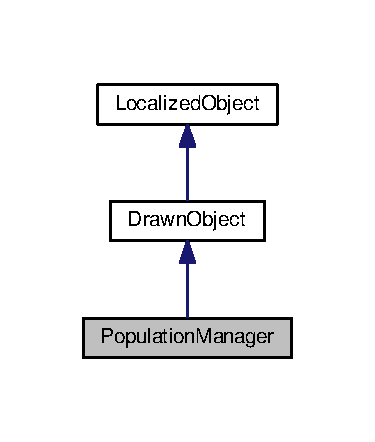
\includegraphics[width=180pt]{classPopulationManager__inherit__graph}
\end{center}
\end{figure}


Collaboration diagram for Population\+Manager\+:\nopagebreak
\begin{figure}[H]
\begin{center}
\leavevmode
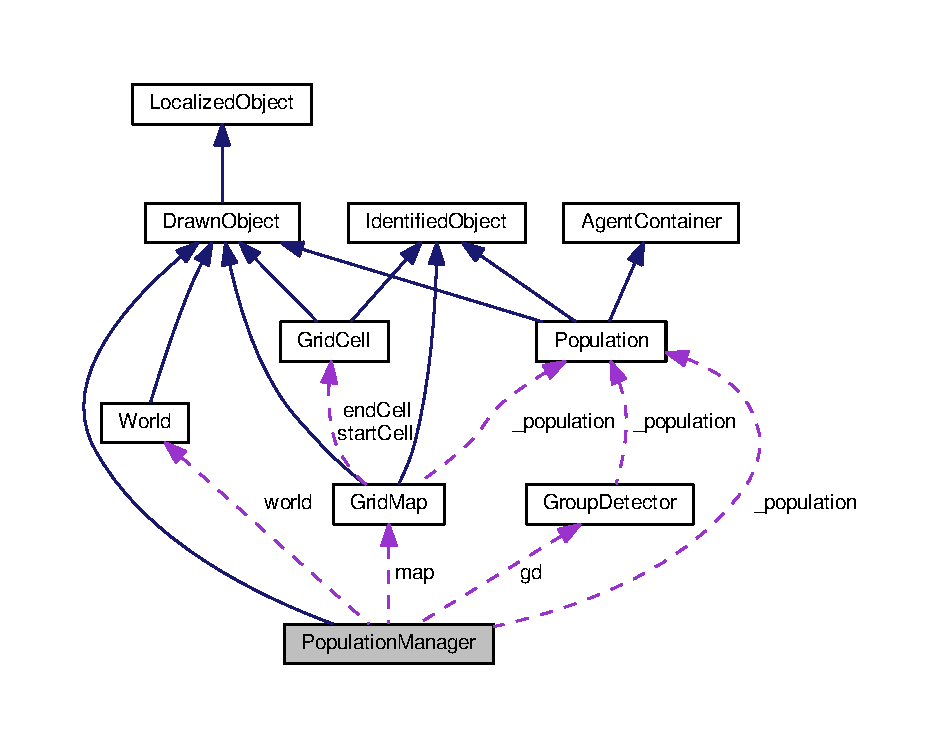
\includegraphics[width=350pt]{classPopulationManager__coll__graph}
\end{center}
\end{figure}
\subsection*{Public Member Functions}
\begin{DoxyCompactItemize}
\item 
{\bfseries Population\+Manager} (\hyperlink{classWorld}{World} $\ast$world)\hypertarget{classPopulationManager_a358c64c798fb4f77958cb45f9da768b1}{}\label{classPopulationManager_a358c64c798fb4f77958cb45f9da768b1}

\item 
{\bfseries Population\+Manager} (\hyperlink{classWorld}{World} $\ast$world, std\+::string feature\+\_\+file, Vector3d p=Vector3d())\hypertarget{classPopulationManager_af6ec5e12d10cda4641e251e5ed873370}{}\label{classPopulationManager_af6ec5e12d10cda4641e251e5ed873370}

\item 
{\bfseries Population\+Manager} (std\+::string feature\+\_\+file, std\+::string gt\+\_\+file, Vector3d p=Vector3d())\hypertarget{classPopulationManager_aa083bdb9f3f534efa38eaa77455af812}{}\label{classPopulationManager_aa083bdb9f3f534efa38eaa77455af812}

\item 
int {\bfseries load\+Frame} (unsigned int f\+Index)\hypertarget{classPopulationManager_a2c893024ba17d5b106490ce9487ba86f}{}\label{classPopulationManager_a2c893024ba17d5b106490ce9487ba86f}

\item 
int {\bfseries load\+Json} ()\hypertarget{classPopulationManager_a08dc1edfd34f15596558e7c8e348e04a}{}\label{classPopulationManager_a08dc1edfd34f15596558e7c8e348e04a}

\item 
int {\bfseries load\+Feature\+Json} ()\hypertarget{classPopulationManager_a01822daf4197ca03f2139e52bbc18da9}{}\label{classPopulationManager_a01822daf4197ca03f2139e52bbc18da9}

\item 
int {\bfseries load\+Ground\+Truth\+Json} ()\hypertarget{classPopulationManager_af3cd5b0b6f3d60def4ed1155cd7b63b6}{}\label{classPopulationManager_af3cd5b0b6f3d60def4ed1155cd7b63b6}

\item 
void {\bfseries find\+Data\+Bounds} ()\hypertarget{classPopulationManager_aea9e6453830edea5dfeb25c591995274}{}\label{classPopulationManager_aea9e6453830edea5dfeb25c591995274}

\item 
\hyperlink{classFormation}{Formation} $\ast$ {\bfseries get\+Highest\+Formation\+Interaction\+Potential} ()\hypertarget{classPopulationManager_ab856989f3b690ed28ec62346f89084a1}{}\label{classPopulationManager_ab856989f3b690ed28ec62346f89084a1}

\item 
void {\bfseries run\+Test} ()\hypertarget{classPopulationManager_af59d2f1328ae10dd0f39bed9f7fd1446}{}\label{classPopulationManager_af59d2f1328ae10dd0f39bed9f7fd1446}

\item 
int {\bfseries next\+Frame} ()\hypertarget{classPopulationManager_adefe1cf12c8235dcbb1b71c4abaf9285}{}\label{classPopulationManager_adefe1cf12c8235dcbb1b71c4abaf9285}

\item 
int {\bfseries previous\+Frame} ()\hypertarget{classPopulationManager_a3cff6a6092f49e9dc1c1ceab1d8ebd02}{}\label{classPopulationManager_a3cff6a6092f49e9dc1c1ceab1d8ebd02}

\item 
void {\bfseries find\+Interaction} ()\hypertarget{classPopulationManager_a11ccb01d3f63cb74fee26876d6fd353a}{}\label{classPopulationManager_a11ccb01d3f63cb74fee26876d6fd353a}

\item 
void {\bfseries draw} (\hyperlink{classWorld}{World} $\ast$world)\hypertarget{classPopulationManager_a7b61ef70b107a5c6ffa7ae811cb2e9f7}{}\label{classPopulationManager_a7b61ef70b107a5c6ffa7ae811cb2e9f7}

\item 
void {\bfseries update} ()\hypertarget{classPopulationManager_aa6911ed18539c497498a824d94c518fa}{}\label{classPopulationManager_aa6911ed18539c497498a824d94c518fa}

\item 
\hyperlink{classPopulation}{Population} $\ast$ {\bfseries get\+Population} () const \hypertarget{classPopulationManager_a004d5657414384945ccd9ce19e052b6b}{}\label{classPopulationManager_a004d5657414384945ccd9ce19e052b6b}

\item 
void {\bfseries set\+Population} (\hyperlink{classPopulation}{Population} $\ast$population)\hypertarget{classPopulationManager_a8a049f79ebad2ca3b95ca830a2cb4ce4}{}\label{classPopulationManager_a8a049f79ebad2ca3b95ca830a2cb4ce4}

\item 
const std\+::string \& {\bfseries get\+Feature\+File} () const \hypertarget{classPopulationManager_a27684ca0d24e28d03e8101d22665cfc7}{}\label{classPopulationManager_a27684ca0d24e28d03e8101d22665cfc7}

\item 
void {\bfseries set\+Feature\+File} (const std\+::string \&feature\+File)\hypertarget{classPopulationManager_a943ed6b0d245b7a067bae3e3bf8b8a76}{}\label{classPopulationManager_a943ed6b0d245b7a067bae3e3bf8b8a76}

\item 
const ofx\+J\+S\+O\+N\+Element \& {\bfseries get\+Features} () const \hypertarget{classPopulationManager_a35e0b3c1dbf718c23ac2132969d270aa}{}\label{classPopulationManager_a35e0b3c1dbf718c23ac2132969d270aa}

\item 
void {\bfseries set\+Features} (const ofx\+J\+S\+O\+N\+Element \&features)\hypertarget{classPopulationManager_ad0f56a78149c12e9327456f8f0264dcb}{}\label{classPopulationManager_ad0f56a78149c12e9327456f8f0264dcb}

\item 
unsigned int {\bfseries get\+Frame\+Index} () const \hypertarget{classPopulationManager_a29ac81f9b477aaeba57ccff9cbe35b48}{}\label{classPopulationManager_a29ac81f9b477aaeba57ccff9cbe35b48}

\item 
void {\bfseries set\+Frame\+Index} (unsigned int frame\+Index)\hypertarget{classPopulationManager_ab442ff6670f1d9ae312949c80c1d2024}{}\label{classPopulationManager_ab442ff6670f1d9ae312949c80c1d2024}

\item 
const ofx\+J\+S\+O\+N\+Element \& {\bfseries get\+Ground\+Truth} () const \hypertarget{classPopulationManager_a50ffc188c034c544f30f8dc47c7f0ed9}{}\label{classPopulationManager_a50ffc188c034c544f30f8dc47c7f0ed9}

\item 
void {\bfseries set\+Ground\+Truth} (const ofx\+J\+S\+O\+N\+Element \&ground\+Truth)\hypertarget{classPopulationManager_a082873088273ed995bdb939dbb1b6af2}{}\label{classPopulationManager_a082873088273ed995bdb939dbb1b6af2}

\item 
bool {\bfseries is\+Gt\+Enabled} () const \hypertarget{classPopulationManager_a7a65e0c78ae942f827d83fe4479ddc78}{}\label{classPopulationManager_a7a65e0c78ae942f827d83fe4479ddc78}

\item 
void {\bfseries set\+Gt\+Enabled} (bool gt\+Enabled)\hypertarget{classPopulationManager_a8ff05f80d5610a5bc4a48e9bafbcb6e0}{}\label{classPopulationManager_a8ff05f80d5610a5bc4a48e9bafbcb6e0}

\item 
const std\+::string \& {\bfseries get\+Gt\+File} () const \hypertarget{classPopulationManager_af92a989024c47451ad1a4af4d6fc3543}{}\label{classPopulationManager_af92a989024c47451ad1a4af4d6fc3543}

\item 
void {\bfseries set\+Gt\+File} (const std\+::string \&gt\+File)\hypertarget{classPopulationManager_a1bc7287c2b14b7895e93b0bcce66637e}{}\label{classPopulationManager_a1bc7287c2b14b7895e93b0bcce66637e}

\item 
bool {\bfseries is\+Loaded} () const \hypertarget{classPopulationManager_a4b241f6ac08df413d02765231f535d18}{}\label{classPopulationManager_a4b241f6ac08df413d02765231f535d18}

\item 
void {\bfseries set\+Loaded} (bool loaded)\hypertarget{classPopulationManager_a8df267c991b192cd7904edfbe483af11}{}\label{classPopulationManager_a8df267c991b192cd7904edfbe483af11}

\item 
\hyperlink{classWorld}{World} $\ast$ {\bfseries get\+World} () const \hypertarget{classPopulationManager_a192c3235326ff9d3dc90809cc89accdd}{}\label{classPopulationManager_a192c3235326ff9d3dc90809cc89accdd}

\item 
\hyperlink{classGridMap}{Grid\+Map} $\ast$ {\bfseries get\+Map} () const \hypertarget{classPopulationManager_a717a85f4fd9702ed4564c7908c694cf1}{}\label{classPopulationManager_a717a85f4fd9702ed4564c7908c694cf1}

\end{DoxyCompactItemize}
\subsection*{Protected Attributes}
\begin{DoxyCompactItemize}
\item 
\hyperlink{classPopulation}{Population} $\ast$ {\bfseries \+\_\+population}\hypertarget{classPopulationManager_a5aeed2477f0858237d62536a79935689}{}\label{classPopulationManager_a5aeed2477f0858237d62536a79935689}

\item 
std\+::vector$<$ \hyperlink{classFormation}{Formation} $\ast$ $>$ {\bfseries \+\_\+\+GT}\hypertarget{classPopulationManager_a71632942b59ad26b92c413545aa50b63}{}\label{classPopulationManager_a71632942b59ad26b92c413545aa50b63}

\item 
ofx\+J\+S\+O\+N\+Element {\bfseries features}\hypertarget{classPopulationManager_ae861d42176c716788ee231a31ca5b64c}{}\label{classPopulationManager_ae861d42176c716788ee231a31ca5b64c}

\item 
ofx\+J\+S\+O\+N\+Element {\bfseries ground\+Truth}\hypertarget{classPopulationManager_af87acc21d7326f4bb3a2d10df99882ad}{}\label{classPopulationManager_af87acc21d7326f4bb3a2d10df99882ad}

\item 
std\+::string {\bfseries feature\+\_\+file}\hypertarget{classPopulationManager_a5944f296dd14faa9d05ffc12fd93edd4}{}\label{classPopulationManager_a5944f296dd14faa9d05ffc12fd93edd4}

\item 
std\+::string {\bfseries gt\+\_\+file}\hypertarget{classPopulationManager_a09c1311b04326acb98e5f4f735ef01c2}{}\label{classPopulationManager_a09c1311b04326acb98e5f4f735ef01c2}

\item 
\hyperlink{classWorld}{World} $\ast$ {\bfseries world}\hypertarget{classPopulationManager_a30865f8987c485caff39f54bbfb6a705}{}\label{classPopulationManager_a30865f8987c485caff39f54bbfb6a705}

\item 
\hyperlink{classGridMap}{Grid\+Map} $\ast$ {\bfseries map}\hypertarget{classPopulationManager_a2388eb51b85c7a74c1bff6e8f61f0a0e}{}\label{classPopulationManager_a2388eb51b85c7a74c1bff6e8f61f0a0e}

\item 
\hyperlink{classGroupDetector}{Group\+Detector} $\ast$ {\bfseries gd}\hypertarget{classPopulationManager_a130877f2f208878998de72f9ee6a6b84}{}\label{classPopulationManager_a130877f2f208878998de72f9ee6a6b84}

\item 
double {\bfseries min\+\_\+x}\hypertarget{classPopulationManager_a7d1b15dc7382fb2c983016a97e5929c2}{}\label{classPopulationManager_a7d1b15dc7382fb2c983016a97e5929c2}

\item 
double {\bfseries min\+\_\+y}\hypertarget{classPopulationManager_a00fa3879b5ab8777413c53c637f90eb0}{}\label{classPopulationManager_a00fa3879b5ab8777413c53c637f90eb0}

\item 
double {\bfseries max\+\_\+x}\hypertarget{classPopulationManager_a4ab5137b2cc1a7b2524bf0762c8e3d0e}{}\label{classPopulationManager_a4ab5137b2cc1a7b2524bf0762c8e3d0e}

\item 
double {\bfseries max\+\_\+y}\hypertarget{classPopulationManager_ab7326fb1c1004354ad4918db911052eb}{}\label{classPopulationManager_ab7326fb1c1004354ad4918db911052eb}

\item 
bool {\bfseries loaded} = 0\hypertarget{classPopulationManager_acf20d29d3095007ef674415702b836f5}{}\label{classPopulationManager_acf20d29d3095007ef674415702b836f5}

\item 
bool {\bfseries gt\+\_\+enabled} = 1\hypertarget{classPopulationManager_a5c34a8449db919ec03bb784d3dd9dc52}{}\label{classPopulationManager_a5c34a8449db919ec03bb784d3dd9dc52}

\item 
unsigned int {\bfseries frame\+Index} = 0\hypertarget{classPopulationManager_ac25b65c23880b06dcafc91de1e3a78a4}{}\label{classPopulationManager_ac25b65c23880b06dcafc91de1e3a78a4}

\end{DoxyCompactItemize}


The documentation for this class was generated from the following files\+:\begin{DoxyCompactItemize}
\item 
src/agent\+Management/Population\+Manager.\+h\item 
src/agent\+Management/Population\+Manager.\+cpp\end{DoxyCompactItemize}

\hypertarget{classRobot}{}\section{Robot Class Reference}
\label{classRobot}\index{Robot@{Robot}}


This class represent the \hyperlink{classRobot}{Robot}.  




{\ttfamily \#include $<$Robot.\+h$>$}



Inheritance diagram for Robot\+:\nopagebreak
\begin{figure}[H]
\begin{center}
\leavevmode
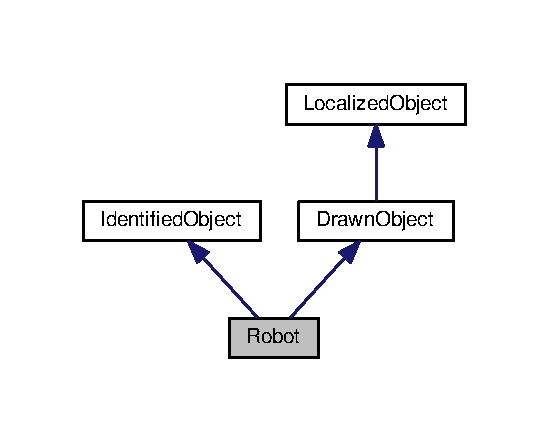
\includegraphics[width=264pt]{classRobot__inherit__graph}
\end{center}
\end{figure}


Collaboration diagram for Robot\+:\nopagebreak
\begin{figure}[H]
\begin{center}
\leavevmode
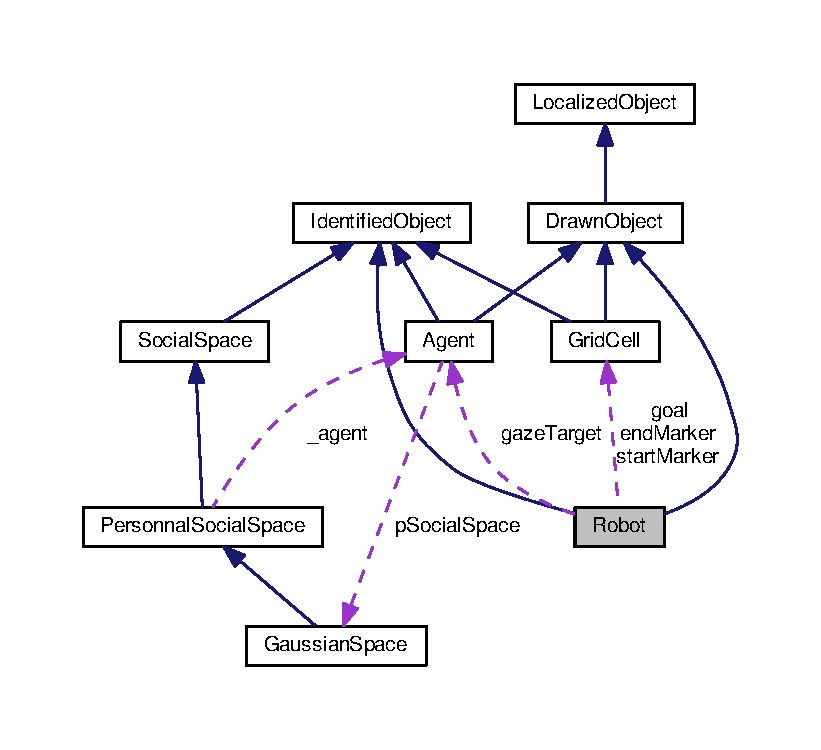
\includegraphics[width=350pt]{classRobot__coll__graph}
\end{center}
\end{figure}
\subsection*{Public Member Functions}
\begin{DoxyCompactItemize}
\item 
\hyperlink{classRobot_a02cded1ec8e6c536a2e07a44d45b3551}{Robot} (Vector3d \hyperlink{classLocalizedObject_a340834deefc9e5c39da1f26c4ebf4f8c}{position}=Vector3d(0, 0, 0), double \hyperlink{classLocalizedObject_aa5f7b070b6dc97a64a90797a0bca56e2}{theta}=0)
\begin{DoxyCompactList}\small\item\em Constructor. \end{DoxyCompactList}\item 
\hyperlink{classRobot_a924320124b09c2f2ac1621aa210d5f38}{$\sim$\+Robot} ()
\begin{DoxyCompactList}\small\item\em Destructor. \end{DoxyCompactList}\item 
void \hyperlink{classRobot_adc34eec22821c2dce23904a5ea75cf13}{update} ()\hypertarget{classRobot_adc34eec22821c2dce23904a5ea75cf13}{}\label{classRobot_adc34eec22821c2dce23904a5ea75cf13}

\begin{DoxyCompactList}\small\item\em Compute the movement and the rotation of the \hyperlink{classRobot}{Robot} based on the computed path and linear interpolation between points. \end{DoxyCompactList}\item 
void \hyperlink{classRobot_a2a169125261257a4900c546c6b9a02b0}{reset\+Path\+Finding} ()\hypertarget{classRobot_a2a169125261257a4900c546c6b9a02b0}{}\label{classRobot_a2a169125261257a4900c546c6b9a02b0}

\begin{DoxyCompactList}\small\item\em Reset path finding process. \end{DoxyCompactList}\item 
\hyperlink{classGridCell}{Grid\+Cell} $\ast$ \hyperlink{classRobot_affcb4c5da6b12767dfcd72c326a7700d}{get\+Goal} () const 
\begin{DoxyCompactList}\small\item\em Simple getter. \end{DoxyCompactList}\item 
void \hyperlink{classRobot_a1217544214600ddd32ff2f060f1bee15}{set\+Goal} (\hyperlink{classGridCell}{Grid\+Cell} $\ast$\hyperlink{classRobot_a5abff8bb9893b5fbd509c20e7fa2ffb5}{goal})
\begin{DoxyCompactList}\small\item\em Simple setter. \end{DoxyCompactList}\item 
std\+::vector$<$ \hyperlink{classGridCell}{Grid\+Cell} $\ast$ $>$ \hyperlink{classRobot_a4b33fb1546feb63a73f75a9c073d6d6f}{get\+Path} () const 
\begin{DoxyCompactList}\small\item\em Simple getter. \end{DoxyCompactList}\item 
void \hyperlink{classRobot_a12b5d95d7764f62b83ed237d18399f13}{set\+Path} (std\+::vector$<$ \hyperlink{classGridCell}{Grid\+Cell} $\ast$ $>$ \hyperlink{classRobot_a6a62d6834a3be1352b81d380cc396e7b}{path})
\begin{DoxyCompactList}\small\item\em Simple setter. \end{DoxyCompactList}\end{DoxyCompactItemize}
\subsection*{Public Attributes}
\begin{DoxyCompactItemize}
\item 
\hyperlink{classGridCell}{Grid\+Cell} $\ast$ \hyperlink{classRobot_a5abff8bb9893b5fbd509c20e7fa2ffb5}{goal}\hypertarget{classRobot_a5abff8bb9893b5fbd509c20e7fa2ffb5}{}\label{classRobot_a5abff8bb9893b5fbd509c20e7fa2ffb5}

\begin{DoxyCompactList}\small\item\em The current goal of the \hyperlink{classRobot}{Robot}. \end{DoxyCompactList}\item 
std\+::vector$<$ \hyperlink{classGridCell}{Grid\+Cell} $\ast$ $>$ \hyperlink{classRobot_a6a62d6834a3be1352b81d380cc396e7b}{path}\hypertarget{classRobot_a6a62d6834a3be1352b81d380cc396e7b}{}\label{classRobot_a6a62d6834a3be1352b81d380cc396e7b}

\begin{DoxyCompactList}\small\item\em The current path followed by the \hyperlink{classRobot}{Robot}. \end{DoxyCompactList}\item 
int \hyperlink{classRobot_a4720ed975e9fae5466f00da717dbb522}{path\+Index}\hypertarget{classRobot_a4720ed975e9fae5466f00da717dbb522}{}\label{classRobot_a4720ed975e9fae5466f00da717dbb522}

\begin{DoxyCompactList}\small\item\em The current path index. \end{DoxyCompactList}\item 
\hyperlink{classGridCell}{Grid\+Cell} $\ast$ \hyperlink{classRobot_afec08358c6c5f12d6d85dfa78a1faa0b}{start\+Marker}\hypertarget{classRobot_afec08358c6c5f12d6d85dfa78a1faa0b}{}\label{classRobot_afec08358c6c5f12d6d85dfa78a1faa0b}

\begin{DoxyCompactList}\small\item\em The starting \hyperlink{classGridCell}{Grid\+Cell}. \end{DoxyCompactList}\item 
\hyperlink{classGridCell}{Grid\+Cell} $\ast$ \hyperlink{classRobot_a6743f0c8b4ae8377d4b275cb452eb924}{end\+Marker}\hypertarget{classRobot_a6743f0c8b4ae8377d4b275cb452eb924}{}\label{classRobot_a6743f0c8b4ae8377d4b275cb452eb924}

\begin{DoxyCompactList}\small\item\em The goal \hyperlink{classGridCell}{Grid\+Cell}. \end{DoxyCompactList}\item 
std\+::chrono\+::time\+\_\+point$<$ std\+::chrono\+::system\+\_\+clock $>$ \hyperlink{classRobot_a4d1fbc7e28a1e3d07bbdfdcc8612a3bf}{start\+Move\+Time}\hypertarget{classRobot_a4d1fbc7e28a1e3d07bbdfdcc8612a3bf}{}\label{classRobot_a4d1fbc7e28a1e3d07bbdfdcc8612a3bf}

\begin{DoxyCompactList}\small\item\em Start time of the movement. \end{DoxyCompactList}\item 
std\+::chrono\+::time\+\_\+point$<$ std\+::chrono\+::system\+\_\+clock $>$ \hyperlink{classRobot_a2eba6b986b51c8197d77bc8c8169fb99}{start\+Rot\+Time}\hypertarget{classRobot_a2eba6b986b51c8197d77bc8c8169fb99}{}\label{classRobot_a2eba6b986b51c8197d77bc8c8169fb99}

\begin{DoxyCompactList}\small\item\em Start time of the rotation. \end{DoxyCompactList}\item 
\hyperlink{classAgent}{Agent} $\ast$ \hyperlink{classRobot_a16adeabd42cf91daf19f7737d7f6c1f3}{gaze\+Target}\hypertarget{classRobot_a16adeabd42cf91daf19f7737d7f6c1f3}{}\label{classRobot_a16adeabd42cf91daf19f7737d7f6c1f3}

\begin{DoxyCompactList}\small\item\em The \hyperlink{classRobot}{Robot} gaze targeted \hyperlink{classAgent}{Agent} for social signals. \end{DoxyCompactList}\item 
double \hyperlink{classRobot_a0d83147dd6fa4db281ed2d6f3c37adf7}{target\+Angle}\hypertarget{classRobot_a0d83147dd6fa4db281ed2d6f3c37adf7}{}\label{classRobot_a0d83147dd6fa4db281ed2d6f3c37adf7}

\begin{DoxyCompactList}\small\item\em The current targeted angle. \end{DoxyCompactList}\item 
double $\ast$ \hyperlink{classRobot_af3df5c8b9901dc8bc721cb0a4fdbc489}{final\+Target\+Angle}\hypertarget{classRobot_af3df5c8b9901dc8bc721cb0a4fdbc489}{}\label{classRobot_af3df5c8b9901dc8bc721cb0a4fdbc489}

\begin{DoxyCompactList}\small\item\em The targeted angle at the end of the movement. \end{DoxyCompactList}\item 
double \hyperlink{classRobot_a6dfebfac8d7ce0da74e9b725b497c525}{start\+Angle}\hypertarget{classRobot_a6dfebfac8d7ce0da74e9b725b497c525}{}\label{classRobot_a6dfebfac8d7ce0da74e9b725b497c525}

\begin{DoxyCompactList}\small\item\em The initial angle of the \hyperlink{classRobot}{Robot}. \end{DoxyCompactList}\item 
double \hyperlink{classRobot_ab79446f46b69d63a3341a4def1e5a043}{rot\+Dist}\hypertarget{classRobot_ab79446f46b69d63a3341a4def1e5a043}{}\label{classRobot_ab79446f46b69d63a3341a4def1e5a043}

\begin{DoxyCompactList}\small\item\em The rotation distance of the actual segment. \end{DoxyCompactList}\item 
double \hyperlink{classRobot_a8f87b634a13863235dd64bdc2ac64eb1}{move\+Dist}\hypertarget{classRobot_a8f87b634a13863235dd64bdc2ac64eb1}{}\label{classRobot_a8f87b634a13863235dd64bdc2ac64eb1}

\begin{DoxyCompactList}\small\item\em The movement distance of the actual segment. \end{DoxyCompactList}\item 
double \hyperlink{classRobot_a4c80046bdc0e2fc0abe63fc8eebb252b}{alpha\+Move} = 0.\+05\hypertarget{classRobot_a4c80046bdc0e2fc0abe63fc8eebb252b}{}\label{classRobot_a4c80046bdc0e2fc0abe63fc8eebb252b}

\begin{DoxyCompactList}\small\item\em Used by the movement formulae. \end{DoxyCompactList}\item 
double \hyperlink{classRobot_ac7f70af1a0589ef3f2964cc1fe17705d}{alpha\+Rot} = 0.\+05\hypertarget{classRobot_ac7f70af1a0589ef3f2964cc1fe17705d}{}\label{classRobot_ac7f70af1a0589ef3f2964cc1fe17705d}

\begin{DoxyCompactList}\small\item\em Used by the rotation formulae. \end{DoxyCompactList}\item 
double \hyperlink{classRobot_a9ffd926d965152cb275765d1abaee1cf}{move\+Speed} = 0.\+5f\hypertarget{classRobot_a9ffd926d965152cb275765d1abaee1cf}{}\label{classRobot_a9ffd926d965152cb275765d1abaee1cf}

\begin{DoxyCompactList}\small\item\em The \hyperlink{classRobot}{Robot} move speed in meter/s. \end{DoxyCompactList}\item 
double \hyperlink{classRobot_ac3f99d1bd98a5d7f65c7d419fe6436b3}{rot\+Speed} = 4.\+0f\hypertarget{classRobot_ac3f99d1bd98a5d7f65c7d419fe6436b3}{}\label{classRobot_ac3f99d1bd98a5d7f65c7d419fe6436b3}

\begin{DoxyCompactList}\small\item\em The \hyperlink{classRobot}{Robot} move speed in radian/s. \end{DoxyCompactList}\item 
bool \hyperlink{classRobot_a8ece8d9045201ce807d1b90e2eb34dd4}{init\+Point} = 1\hypertarget{classRobot_a8ece8d9045201ce807d1b90e2eb34dd4}{}\label{classRobot_a8ece8d9045201ce807d1b90e2eb34dd4}

\begin{DoxyCompactList}\small\item\em Enable or disable path finding segment initialization. \end{DoxyCompactList}\end{DoxyCompactItemize}
\subsection*{Additional Inherited Members}


\subsection{Detailed Description}
This class represent the \hyperlink{classRobot}{Robot}. 

This class manage the \hyperlink{classRobot}{Robot} and its movement 

\subsection{Constructor \& Destructor Documentation}
\index{Robot@{Robot}!Robot@{Robot}}
\index{Robot@{Robot}!Robot@{Robot}}
\subsubsection[{\texorpdfstring{Robot(\+Vector3d position=\+Vector3d(0, 0, 0), double theta=0)}{Robot(Vector3d position=Vector3d(0, 0, 0), double theta=0)}}]{\setlength{\rightskip}{0pt plus 5cm}Robot\+::\+Robot (
\begin{DoxyParamCaption}
\item[{Vector3d}]{position = {\ttfamily Vector3d(0,0,0)}, }
\item[{double}]{theta = {\ttfamily 0}}
\end{DoxyParamCaption}
)}\hypertarget{classRobot_a02cded1ec8e6c536a2e07a44d45b3551}{}\label{classRobot_a02cded1ec8e6c536a2e07a44d45b3551}


Constructor. 

Constructor of the \hyperlink{classRobot}{Robot} class


\begin{DoxyParams}{Parameters}
{\em position} & \+: Initial position of the \hyperlink{classRobot}{Robot} in \hyperlink{classWorld}{World} \\
\hline
{\em theta} & \+: Initial angle of the \hyperlink{classRobot}{Robot} \\
\hline
\end{DoxyParams}
\index{Robot@{Robot}!````~Robot@{$\sim$\+Robot}}
\index{````~Robot@{$\sim$\+Robot}!Robot@{Robot}}
\subsubsection[{\texorpdfstring{$\sim$\+Robot()}{~Robot()}}]{\setlength{\rightskip}{0pt plus 5cm}Robot\+::$\sim$\+Robot (
\begin{DoxyParamCaption}
{}
\end{DoxyParamCaption}
)}\hypertarget{classRobot_a924320124b09c2f2ac1621aa210d5f38}{}\label{classRobot_a924320124b09c2f2ac1621aa210d5f38}


Destructor. 

Destructor of the \hyperlink{classRobot}{Robot} class 

\subsection{Member Function Documentation}
\index{Robot@{Robot}!get\+Goal@{get\+Goal}}
\index{get\+Goal@{get\+Goal}!Robot@{Robot}}
\subsubsection[{\texorpdfstring{get\+Goal() const }{getGoal() const }}]{\setlength{\rightskip}{0pt plus 5cm}{\bf Grid\+Cell} $\ast$ Robot\+::get\+Goal (
\begin{DoxyParamCaption}
{}
\end{DoxyParamCaption}
) const}\hypertarget{classRobot_affcb4c5da6b12767dfcd72c326a7700d}{}\label{classRobot_affcb4c5da6b12767dfcd72c326a7700d}


Simple getter. 

\begin{DoxyReturn}{Returns}
goal 
\end{DoxyReturn}
\index{Robot@{Robot}!get\+Path@{get\+Path}}
\index{get\+Path@{get\+Path}!Robot@{Robot}}
\subsubsection[{\texorpdfstring{get\+Path() const }{getPath() const }}]{\setlength{\rightskip}{0pt plus 5cm}std\+::vector$<$ {\bf Grid\+Cell} $\ast$ $>$ Robot\+::get\+Path (
\begin{DoxyParamCaption}
{}
\end{DoxyParamCaption}
) const}\hypertarget{classRobot_a4b33fb1546feb63a73f75a9c073d6d6f}{}\label{classRobot_a4b33fb1546feb63a73f75a9c073d6d6f}


Simple getter. 

\begin{DoxyReturn}{Returns}
path 
\end{DoxyReturn}
\index{Robot@{Robot}!set\+Goal@{set\+Goal}}
\index{set\+Goal@{set\+Goal}!Robot@{Robot}}
\subsubsection[{\texorpdfstring{set\+Goal(\+Grid\+Cell $\ast$goal)}{setGoal(GridCell *goal)}}]{\setlength{\rightskip}{0pt plus 5cm}void Robot\+::set\+Goal (
\begin{DoxyParamCaption}
\item[{{\bf Grid\+Cell} $\ast$}]{goal}
\end{DoxyParamCaption}
)}\hypertarget{classRobot_a1217544214600ddd32ff2f060f1bee15}{}\label{classRobot_a1217544214600ddd32ff2f060f1bee15}


Simple setter. 


\begin{DoxyParams}{Parameters}
{\em goal} & \\
\hline
\end{DoxyParams}
\index{Robot@{Robot}!set\+Path@{set\+Path}}
\index{set\+Path@{set\+Path}!Robot@{Robot}}
\subsubsection[{\texorpdfstring{set\+Path(std\+::vector$<$ Grid\+Cell $\ast$ $>$ path)}{setPath(std::vector< GridCell * > path)}}]{\setlength{\rightskip}{0pt plus 5cm}void Robot\+::set\+Path (
\begin{DoxyParamCaption}
\item[{std\+::vector$<$ {\bf Grid\+Cell} $\ast$ $>$}]{path}
\end{DoxyParamCaption}
)}\hypertarget{classRobot_a12b5d95d7764f62b83ed237d18399f13}{}\label{classRobot_a12b5d95d7764f62b83ed237d18399f13}


Simple setter. 


\begin{DoxyParams}{Parameters}
{\em path} & \\
\hline
\end{DoxyParams}


The documentation for this class was generated from the following files\+:\begin{DoxyCompactItemize}
\item 
src/agent\+Management/\hyperlink{Robot_8h}{Robot.\+h}\item 
src/agent\+Management/Robot.\+cpp\end{DoxyCompactItemize}

\hypertarget{classSocialPlanner}{}\section{Social\+Planner Class Reference}
\label{classSocialPlanner}\index{Social\+Planner@{Social\+Planner}}


This class is a state machine controlling the \hyperlink{classRobot}{Robot} behavior.  




{\ttfamily \#include $<$Social\+Planner.\+h$>$}



Collaboration diagram for Social\+Planner\+:\nopagebreak
\begin{figure}[H]
\begin{center}
\leavevmode
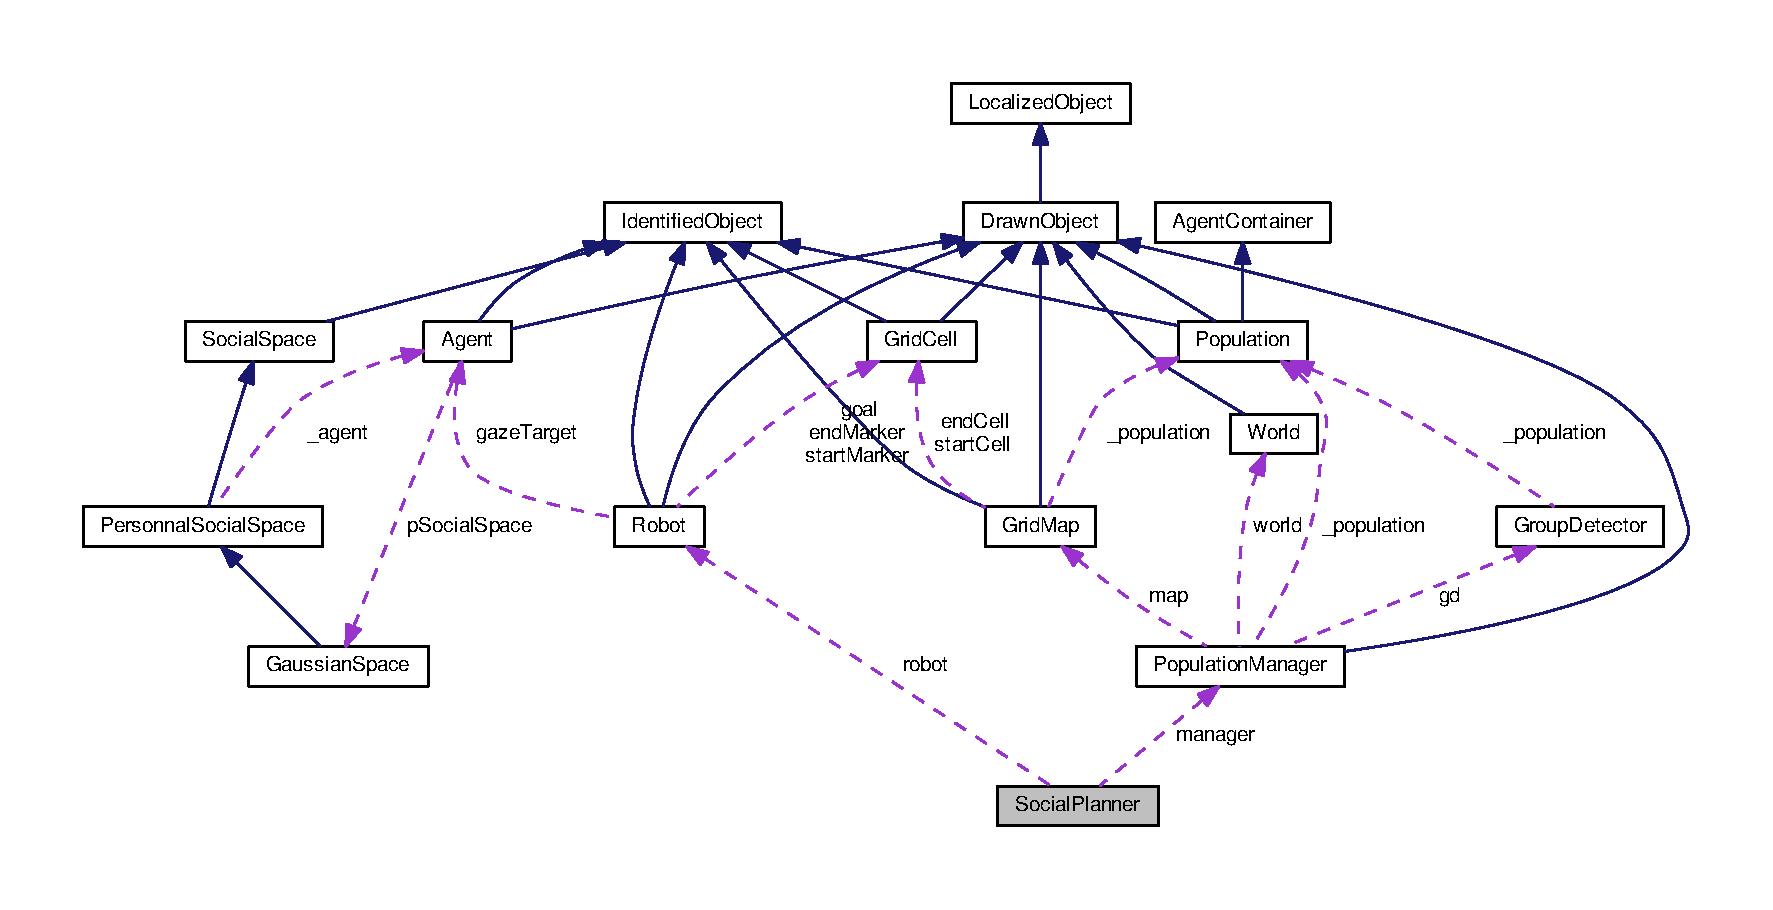
\includegraphics[width=350pt]{classSocialPlanner__coll__graph}
\end{center}
\end{figure}
\subsection*{Public Types}
\begin{DoxyCompactItemize}
\item 
enum \hyperlink{classSocialPlanner_acb2c5c7ab803cafef828f504b1df5f6d}{Social\+State} \{ {\bfseries S\+E\+E\+K\+\_\+\+I\+N\+T\+E\+R\+A\+C\+T\+I\+ON}, 
{\bfseries E\+N\+G\+A\+G\+E\+M\+E\+NT}, 
{\bfseries I\+N\+T\+E\+R\+A\+C\+T\+I\+ON}, 
{\bfseries D\+I\+S\+E\+N\+G\+A\+GE}
 \}\hypertarget{classSocialPlanner_acb2c5c7ab803cafef828f504b1df5f6d}{}\label{classSocialPlanner_acb2c5c7ab803cafef828f504b1df5f6d}
\begin{DoxyCompactList}\small\item\em The states available for the state machine. \end{DoxyCompactList}
\end{DoxyCompactItemize}
\subsection*{Public Member Functions}
\begin{DoxyCompactItemize}
\item 
\hyperlink{classSocialPlanner_ac2225f2890a3b8714d1a00d7c9a7a6c5}{Social\+Planner} (\hyperlink{classPopulationManager}{Population\+Manager} $\ast$pop\+Manager, \hyperlink{classRobot}{Robot} $\ast$\hyperlink{classSocialPlanner_a5f858fb49f0ce512d6a1d524af25d1ff}{robot})
\begin{DoxyCompactList}\small\item\em Constructor. \end{DoxyCompactList}\item 
virtual \hyperlink{classSocialPlanner_a5a6945c1e568005863a533467c2e6ae7}{$\sim$\+Social\+Planner} ()
\begin{DoxyCompactList}\small\item\em Destructor. \end{DoxyCompactList}\item 
void \hyperlink{classSocialPlanner_af5691bba77fe5d5070b2e0853fb79b5b}{update} ()
\begin{DoxyCompactList}\small\item\em Update the state of the robot behavior,. \end{DoxyCompactList}\item 
void \hyperlink{classSocialPlanner_a687dfc247b8d45945a85d0a91b576bbf}{seek\+\_\+interaction} ()
\begin{DoxyCompactList}\small\item\em Seek interaction state. \end{DoxyCompactList}\item 
void \hyperlink{classSocialPlanner_a5dc204e21fd2f4ed915e747f0132d2b4}{engage} ()
\begin{DoxyCompactList}\small\item\em Engage state. \end{DoxyCompactList}\item 
void \hyperlink{classSocialPlanner_a933dd6fd8dbc7f0734b041ab9523d49e}{interact} ()
\begin{DoxyCompactList}\small\item\em Interaction state. \end{DoxyCompactList}\item 
void \hyperlink{classSocialPlanner_abe00dd899b52d575bbd37663e6154967}{disengage} ()
\begin{DoxyCompactList}\small\item\em Disengage state. \end{DoxyCompactList}\item 
\hyperlink{classPopulationManager}{Population\+Manager} $\ast$ \hyperlink{classSocialPlanner_a0b0604374eaf862ddaedcf52a9ab163d}{get\+Manager} () const 
\begin{DoxyCompactList}\small\item\em Simple getter. \end{DoxyCompactList}\item 
\hyperlink{classRobot}{Robot} $\ast$ \hyperlink{classSocialPlanner_a552ff2abf5af651b3adf02b58c144806}{get\+Robot} () const 
\begin{DoxyCompactList}\small\item\em Simple getter. \end{DoxyCompactList}\end{DoxyCompactItemize}
\subsection*{Public Attributes}
\begin{DoxyCompactItemize}
\item 
bool \hyperlink{classSocialPlanner_a13bcec9af0fe2827d8cb1054ea20b591}{interaction\+Started} = 0\hypertarget{classSocialPlanner_a13bcec9af0fe2827d8cb1054ea20b591}{}\label{classSocialPlanner_a13bcec9af0fe2827d8cb1054ea20b591}

\begin{DoxyCompactList}\small\item\em Interaction state started. \end{DoxyCompactList}\item 
bool \hyperlink{classSocialPlanner_abb314ece6c333d6afc821f9a040b38ae}{seek\+Started} = 0\hypertarget{classSocialPlanner_abb314ece6c333d6afc821f9a040b38ae}{}\label{classSocialPlanner_abb314ece6c333d6afc821f9a040b38ae}

\begin{DoxyCompactList}\small\item\em Seek interaction state started. \end{DoxyCompactList}\item 
std\+::chrono\+::time\+\_\+point$<$ std\+::chrono\+::system\+\_\+clock $>$ \hyperlink{classSocialPlanner_ab22aaaf906f821e511c7703a4b663442}{start\+Interaction\+Time}\hypertarget{classSocialPlanner_ab22aaaf906f821e511c7703a4b663442}{}\label{classSocialPlanner_ab22aaaf906f821e511c7703a4b663442}

\begin{DoxyCompactList}\small\item\em Time when interaction state started. \end{DoxyCompactList}\item 
std\+::chrono\+::time\+\_\+point$<$ std\+::chrono\+::system\+\_\+clock $>$ \hyperlink{classSocialPlanner_a80652fac5bcf138d82f9b80674a9e922}{start\+Seek\+Time}\hypertarget{classSocialPlanner_a80652fac5bcf138d82f9b80674a9e922}{}\label{classSocialPlanner_a80652fac5bcf138d82f9b80674a9e922}

\begin{DoxyCompactList}\small\item\em Time when seek interaction state started. \end{DoxyCompactList}\item 
std\+::chrono\+::time\+\_\+point$<$ std\+::chrono\+::system\+\_\+clock $>$ \hyperlink{classSocialPlanner_ae727d2e77b91cb5bf494249611dd86d0}{start\+Mutual\+Facial\+Gaze}\hypertarget{classSocialPlanner_ae727d2e77b91cb5bf494249611dd86d0}{}\label{classSocialPlanner_ae727d2e77b91cb5bf494249611dd86d0}

\begin{DoxyCompactList}\small\item\em Time when mutual facial gaze started. \end{DoxyCompactList}\item 
\hyperlink{classSocialPlanner_acb2c5c7ab803cafef828f504b1df5f6d}{Social\+State} \hyperlink{classSocialPlanner_aeadee6941dc26e6ffcbfa5ed13b96cd0}{state} = S\+E\+E\+K\+\_\+\+I\+N\+T\+E\+R\+A\+C\+T\+I\+ON\hypertarget{classSocialPlanner_aeadee6941dc26e6ffcbfa5ed13b96cd0}{}\label{classSocialPlanner_aeadee6941dc26e6ffcbfa5ed13b96cd0}

\begin{DoxyCompactList}\small\item\em Actual state, default is S\+E\+E\+K\+\_\+\+I\+N\+T\+E\+R\+A\+C\+T\+I\+ON. \end{DoxyCompactList}\item 
\hyperlink{classPopulationManager}{Population\+Manager} $\ast$ \hyperlink{classSocialPlanner_aaed8a44f9e82ca53141f6a556365754a}{manager}\hypertarget{classSocialPlanner_aaed8a44f9e82ca53141f6a556365754a}{}\label{classSocialPlanner_aaed8a44f9e82ca53141f6a556365754a}

\begin{DoxyCompactList}\small\item\em The \hyperlink{classPopulationManager}{Population\+Manager} used by the \hyperlink{classSocialPlanner}{Social\+Planner}. \end{DoxyCompactList}\item 
\hyperlink{classRobot}{Robot} $\ast$ \hyperlink{classSocialPlanner_a5f858fb49f0ce512d6a1d524af25d1ff}{robot}\hypertarget{classSocialPlanner_a5f858fb49f0ce512d6a1d524af25d1ff}{}\label{classSocialPlanner_a5f858fb49f0ce512d6a1d524af25d1ff}

\begin{DoxyCompactList}\small\item\em The \hyperlink{classRobot}{Robot} controlled by the \hyperlink{classSocialPlanner}{Social\+Planner}. \end{DoxyCompactList}\item 
Vector3d \hyperlink{classSocialPlanner_ab105a0b94b629c396eaa4837c7234d27}{saved\+Position}\hypertarget{classSocialPlanner_ab105a0b94b629c396eaa4837c7234d27}{}\label{classSocialPlanner_ab105a0b94b629c396eaa4837c7234d27}

\begin{DoxyCompactList}\small\item\em Interaction position saved, dirty. \end{DoxyCompactList}\item 
int \hyperlink{classSocialPlanner_a82d7052c76abb4c2f233484ba60f3398}{gaze\+Target\+Index} = 0\hypertarget{classSocialPlanner_a82d7052c76abb4c2f233484ba60f3398}{}\label{classSocialPlanner_a82d7052c76abb4c2f233484ba60f3398}

\begin{DoxyCompactList}\small\item\em \hyperlink{classAgent}{Agent} index for the gaze target. \end{DoxyCompactList}\end{DoxyCompactItemize}


\subsection{Detailed Description}
This class is a state machine controlling the \hyperlink{classRobot}{Robot} behavior. 

\begin{DoxyRefDesc}{Todo}
\item[\hyperlink{todo__todo000003}{Todo}]This class should be an interface to implement different behavior for the robot \end{DoxyRefDesc}


\subsection{Constructor \& Destructor Documentation}
\index{Social\+Planner@{Social\+Planner}!Social\+Planner@{Social\+Planner}}
\index{Social\+Planner@{Social\+Planner}!Social\+Planner@{Social\+Planner}}
\subsubsection[{\texorpdfstring{Social\+Planner(\+Population\+Manager $\ast$pop\+Manager, Robot $\ast$robot)}{SocialPlanner(PopulationManager *popManager, Robot *robot)}}]{\setlength{\rightskip}{0pt plus 5cm}Social\+Planner\+::\+Social\+Planner (
\begin{DoxyParamCaption}
\item[{{\bf Population\+Manager} $\ast$}]{pop\+Manager, }
\item[{{\bf Robot} $\ast$}]{robot}
\end{DoxyParamCaption}
)}\hypertarget{classSocialPlanner_ac2225f2890a3b8714d1a00d7c9a7a6c5}{}\label{classSocialPlanner_ac2225f2890a3b8714d1a00d7c9a7a6c5}


Constructor. 

Constructor of the \hyperlink{classSocialPlanner}{Social\+Planner} class


\begin{DoxyParams}{Parameters}
{\em pop\+Manager} & \+: The \hyperlink{classPopulation}{Population} where the robot evolves \\
\hline
{\em robot} & \+: The \hyperlink{classRobot}{Robot} controlled by this behavior \\
\hline
\end{DoxyParams}
\index{Social\+Planner@{Social\+Planner}!````~Social\+Planner@{$\sim$\+Social\+Planner}}
\index{````~Social\+Planner@{$\sim$\+Social\+Planner}!Social\+Planner@{Social\+Planner}}
\subsubsection[{\texorpdfstring{$\sim$\+Social\+Planner()}{~SocialPlanner()}}]{\setlength{\rightskip}{0pt plus 5cm}Social\+Planner\+::$\sim$\+Social\+Planner (
\begin{DoxyParamCaption}
{}
\end{DoxyParamCaption}
)\hspace{0.3cm}{\ttfamily [virtual]}}\hypertarget{classSocialPlanner_a5a6945c1e568005863a533467c2e6ae7}{}\label{classSocialPlanner_a5a6945c1e568005863a533467c2e6ae7}


Destructor. 

Destructor of the \hyperlink{classSocialPlanner}{Social\+Planner} class 

\subsection{Member Function Documentation}
\index{Social\+Planner@{Social\+Planner}!disengage@{disengage}}
\index{disengage@{disengage}!Social\+Planner@{Social\+Planner}}
\subsubsection[{\texorpdfstring{disengage()}{disengage()}}]{\setlength{\rightskip}{0pt plus 5cm}void Social\+Planner\+::disengage (
\begin{DoxyParamCaption}
{}
\end{DoxyParamCaption}
)}\hypertarget{classSocialPlanner_abe00dd899b52d575bbd37663e6154967}{}\label{classSocialPlanner_abe00dd899b52d575bbd37663e6154967}


Disengage state. 

The robot ends the interaction by going back to the seek interaction state

\begin{DoxyRefDesc}{Todo}
\item[\hyperlink{todo__todo000004}{Todo}]Execute some social signals for disengagement \end{DoxyRefDesc}
\index{Social\+Planner@{Social\+Planner}!engage@{engage}}
\index{engage@{engage}!Social\+Planner@{Social\+Planner}}
\subsubsection[{\texorpdfstring{engage()}{engage()}}]{\setlength{\rightskip}{0pt plus 5cm}void Social\+Planner\+::engage (
\begin{DoxyParamCaption}
{}
\end{DoxyParamCaption}
)}\hypertarget{classSocialPlanner_a5dc204e21fd2f4ed915e747f0132d2b4}{}\label{classSocialPlanner_a5dc204e21fd2f4ed915e747f0132d2b4}


Engage state. 

The robot move to the interaction position related to the \hyperlink{classFormation}{Formation} and process some social signal like mutual facial gaze to communicate its intentions. And switch to the interaction state when the goal is reached \index{Social\+Planner@{Social\+Planner}!get\+Manager@{get\+Manager}}
\index{get\+Manager@{get\+Manager}!Social\+Planner@{Social\+Planner}}
\subsubsection[{\texorpdfstring{get\+Manager() const }{getManager() const }}]{\setlength{\rightskip}{0pt plus 5cm}{\bf Population\+Manager} $\ast$ Social\+Planner\+::get\+Manager (
\begin{DoxyParamCaption}
{}
\end{DoxyParamCaption}
) const}\hypertarget{classSocialPlanner_a0b0604374eaf862ddaedcf52a9ab163d}{}\label{classSocialPlanner_a0b0604374eaf862ddaedcf52a9ab163d}


Simple getter. 

\begin{DoxyReturn}{Returns}
\hyperlink{classPopulationManager}{Population\+Manager} 
\end{DoxyReturn}
\index{Social\+Planner@{Social\+Planner}!get\+Robot@{get\+Robot}}
\index{get\+Robot@{get\+Robot}!Social\+Planner@{Social\+Planner}}
\subsubsection[{\texorpdfstring{get\+Robot() const }{getRobot() const }}]{\setlength{\rightskip}{0pt plus 5cm}{\bf Robot} $\ast$ Social\+Planner\+::get\+Robot (
\begin{DoxyParamCaption}
{}
\end{DoxyParamCaption}
) const}\hypertarget{classSocialPlanner_a552ff2abf5af651b3adf02b58c144806}{}\label{classSocialPlanner_a552ff2abf5af651b3adf02b58c144806}


Simple getter. 

\begin{DoxyReturn}{Returns}
\hyperlink{classRobot}{Robot} 
\end{DoxyReturn}
\index{Social\+Planner@{Social\+Planner}!interact@{interact}}
\index{interact@{interact}!Social\+Planner@{Social\+Planner}}
\subsubsection[{\texorpdfstring{interact()}{interact()}}]{\setlength{\rightskip}{0pt plus 5cm}void Social\+Planner\+::interact (
\begin{DoxyParamCaption}
{}
\end{DoxyParamCaption}
)}\hypertarget{classSocialPlanner_a933dd6fd8dbc7f0734b041ab9523d49e}{}\label{classSocialPlanner_a933dd6fd8dbc7f0734b041ab9523d49e}


Interaction state. 

The robot simulate an interaction with the \hyperlink{classFormation}{Formation} for I\+N\+T\+E\+R\+A\+C\+T\+I\+O\+N\+\_\+\+M\+A\+X\+\_\+\+T\+I\+ME, then switch to the disengage state. \index{Social\+Planner@{Social\+Planner}!seek\+\_\+interaction@{seek\+\_\+interaction}}
\index{seek\+\_\+interaction@{seek\+\_\+interaction}!Social\+Planner@{Social\+Planner}}
\subsubsection[{\texorpdfstring{seek\+\_\+interaction()}{seek_interaction()}}]{\setlength{\rightskip}{0pt plus 5cm}void Social\+Planner\+::seek\+\_\+interaction (
\begin{DoxyParamCaption}
{}
\end{DoxyParamCaption}
)}\hypertarget{classSocialPlanner_a687dfc247b8d45945a85d0a91b576bbf}{}\label{classSocialPlanner_a687dfc247b8d45945a85d0a91b576bbf}


Seek interaction state. 

The robot is looking for interaction, it goes randomly around the \hyperlink{classGridMap}{Grid\+Map} and after S\+E\+E\+K\+\_\+\+I\+N\+T\+E\+R\+A\+C\+T\+I\+O\+N\+\_\+\+M\+I\+N\+\_\+\+T\+I\+ME it looks for the highest interaction potential available in the formations superior to I\+N\+T\+E\+R\+A\+C\+T\+I\+O\+N\+\_\+\+P\+O\+T\+E\+N\+T\+I\+A\+L\+\_\+\+T\+H\+R\+E\+S\+H\+O\+LD then switch to the engage state \index{Social\+Planner@{Social\+Planner}!update@{update}}
\index{update@{update}!Social\+Planner@{Social\+Planner}}
\subsubsection[{\texorpdfstring{update()}{update()}}]{\setlength{\rightskip}{0pt plus 5cm}void Social\+Planner\+::update (
\begin{DoxyParamCaption}
{}
\end{DoxyParamCaption}
)}\hypertarget{classSocialPlanner_af5691bba77fe5d5070b2e0853fb79b5b}{}\label{classSocialPlanner_af5691bba77fe5d5070b2e0853fb79b5b}


Update the state of the robot behavior,. 

Update the state of the robot behavior, by executing the function related to its actual state 

The documentation for this class was generated from the following files\+:\begin{DoxyCompactItemize}
\item 
src/social\+Processing/\hyperlink{SocialPlanner_8h}{Social\+Planner.\+h}\item 
src/social\+Processing/\hyperlink{SocialPlanner_8cpp}{Social\+Planner.\+cpp}\end{DoxyCompactItemize}

\hypertarget{classSocialSpace}{}\section{Social\+Space Class Reference}
\label{classSocialSpace}\index{Social\+Space@{Social\+Space}}


This class is an abstract class for representing \hyperlink{classSocialSpace}{Social\+Space}.  




{\ttfamily \#include $<$Social\+Space.\+h$>$}



Inheritance diagram for Social\+Space\+:\nopagebreak
\begin{figure}[H]
\begin{center}
\leavevmode
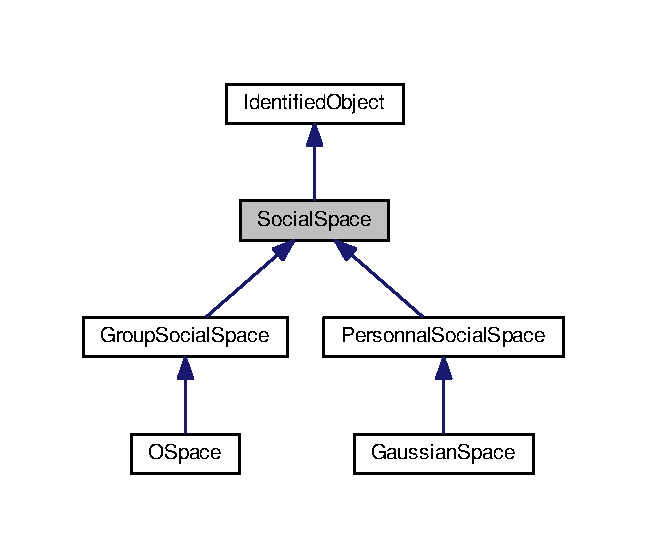
\includegraphics[width=311pt]{classSocialSpace__inherit__graph}
\end{center}
\end{figure}


Collaboration diagram for Social\+Space\+:\nopagebreak
\begin{figure}[H]
\begin{center}
\leavevmode
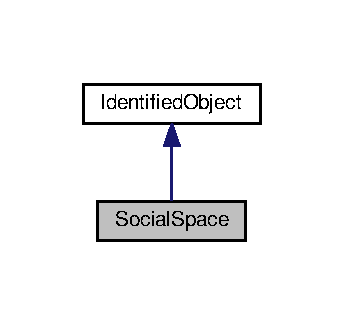
\includegraphics[width=165pt]{classSocialSpace__coll__graph}
\end{center}
\end{figure}
\subsection*{Public Member Functions}
\begin{DoxyCompactItemize}
\item 
\hyperlink{classSocialSpace_a53ab74e94a21331d2a37272cf7bcede1}{Social\+Space} (int \hyperlink{classIdentifiedObject_ad044a317a9b573a3d1bcd025df166eb5}{id}=0)
\begin{DoxyCompactList}\small\item\em Constructor. \end{DoxyCompactList}\item 
virtual \hyperlink{classSocialSpace_a03b060befa0440eddd2ef9d934ac6523}{$\sim$\+Social\+Space} ()
\begin{DoxyCompactList}\small\item\em Destructor. \end{DoxyCompactList}\end{DoxyCompactItemize}
\subsection*{Additional Inherited Members}


\subsection{Detailed Description}
This class is an abstract class for representing \hyperlink{classSocialSpace}{Social\+Space}. 

\subsection{Constructor \& Destructor Documentation}
\index{Social\+Space@{Social\+Space}!Social\+Space@{Social\+Space}}
\index{Social\+Space@{Social\+Space}!Social\+Space@{Social\+Space}}
\subsubsection[{\texorpdfstring{Social\+Space(int id=0)}{SocialSpace(int id=0)}}]{\setlength{\rightskip}{0pt plus 5cm}Social\+Space\+::\+Social\+Space (
\begin{DoxyParamCaption}
\item[{int}]{id = {\ttfamily 0}}
\end{DoxyParamCaption}
)}\hypertarget{classSocialSpace_a53ab74e94a21331d2a37272cf7bcede1}{}\label{classSocialSpace_a53ab74e94a21331d2a37272cf7bcede1}


Constructor. 

Constructor of the \hyperlink{classSocialSpace}{Social\+Space} class


\begin{DoxyParams}{Parameters}
{\em id} & \+: The unique identifier of the \hyperlink{classSocialSpace}{Social\+Space} \\
\hline
\end{DoxyParams}
\index{Social\+Space@{Social\+Space}!````~Social\+Space@{$\sim$\+Social\+Space}}
\index{````~Social\+Space@{$\sim$\+Social\+Space}!Social\+Space@{Social\+Space}}
\subsubsection[{\texorpdfstring{$\sim$\+Social\+Space()}{~SocialSpace()}}]{\setlength{\rightskip}{0pt plus 5cm}Social\+Space\+::$\sim$\+Social\+Space (
\begin{DoxyParamCaption}
{}
\end{DoxyParamCaption}
)\hspace{0.3cm}{\ttfamily [virtual]}}\hypertarget{classSocialSpace_a03b060befa0440eddd2ef9d934ac6523}{}\label{classSocialSpace_a03b060befa0440eddd2ef9d934ac6523}


Destructor. 

Destructor of the \hyperlink{classSocialSpace}{Social\+Space} class 

The documentation for this class was generated from the following files\+:\begin{DoxyCompactItemize}
\item 
src/social\+Space/\hyperlink{SocialSpace_8h}{Social\+Space.\+h}\item 
src/social\+Space/\hyperlink{SocialSpace_8cpp}{Social\+Space.\+cpp}\end{DoxyCompactItemize}

\hypertarget{classUDPServer}{}\section{U\+D\+P\+Server Class Reference}
\label{classUDPServer}\index{U\+D\+P\+Server@{U\+D\+P\+Server}}


This class manage the U\+DP Server sending computed data to a visualization software and receiving \hyperlink{classAgent}{Agent} data from other sensor sources.  




{\ttfamily \#include $<$U\+D\+P\+Server.\+h$>$}



Collaboration diagram for U\+D\+P\+Server\+:\nopagebreak
\begin{figure}[H]
\begin{center}
\leavevmode
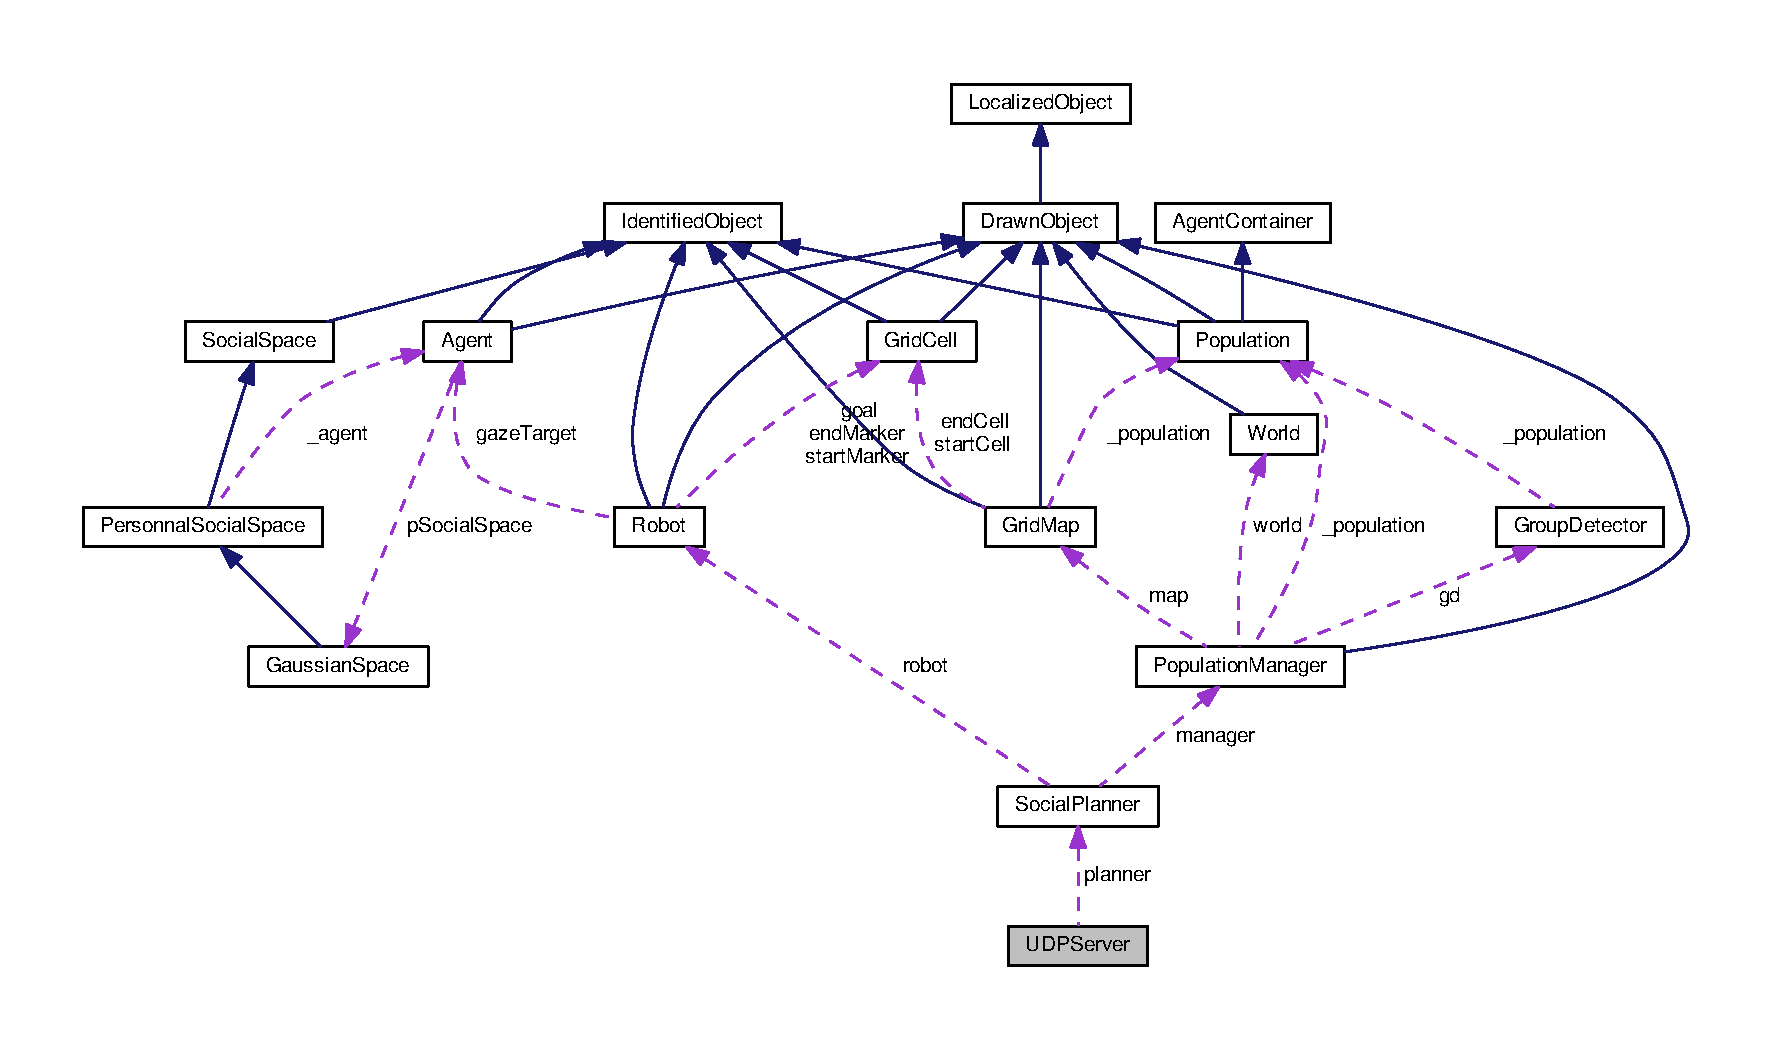
\includegraphics[width=350pt]{classUDPServer__coll__graph}
\end{center}
\end{figure}
\subsection*{Public Member Functions}
\begin{DoxyCompactItemize}
\item 
\hyperlink{classUDPServer_a50889d5ad89f209c9894084a34f82e3b}{U\+D\+P\+Server} (int port, \hyperlink{classSocialPlanner}{Social\+Planner} $\ast$s\+Planner)
\begin{DoxyCompactList}\small\item\em Constructor. \end{DoxyCompactList}\item 
virtual \hyperlink{classUDPServer_a09b1a38f1a03d3832f85fe05e6370a11}{$\sim$\+U\+D\+P\+Server} ()
\begin{DoxyCompactList}\small\item\em Destructor. \end{DoxyCompactList}\item 
std\+::thread \hyperlink{classUDPServer_a854b519058c67d57546486bcc9c50de9}{spawn} ()
\begin{DoxyCompactList}\small\item\em Launch the \hyperlink{classUDPServer}{U\+D\+P\+Server} receive function in a new thread. \end{DoxyCompactList}\item 
int \hyperlink{classUDPServer_ae819b033ef968a8231ed1413da3c46d5}{parse} ()
\begin{DoxyCompactList}\small\item\em Parse the data received by the receive thread. \end{DoxyCompactList}\item 
int \hyperlink{classUDPServer_a215a250437888719487938c72ce3225c}{parse\+\_\+frame0} ()
\begin{DoxyCompactList}\small\item\em Parse frame0 containing \hyperlink{classAgent}{Agent} data. \end{DoxyCompactList}\item 
int \hyperlink{classUDPServer_a5303b2aeaec59beafd748d2938b807a2}{send\+\_\+frame0} ()
\begin{DoxyCompactList}\small\item\em Create frame0 containing all \hyperlink{classAgent}{Agent} data from the \hyperlink{classPopulation}{Population}. \end{DoxyCompactList}\item 
int \hyperlink{classUDPServer_adcbe3797150866d0c82e00941555da38}{send\+\_\+frame1} ()
\begin{DoxyCompactList}\small\item\em Create frame1 containing the \hyperlink{classRobot}{Robot} data. \end{DoxyCompactList}\item 
int \hyperlink{classUDPServer_a79979deab54cb01a0b50ada969671d56}{send\+\_\+frame2} ()
\begin{DoxyCompactList}\small\item\em Create frame2 containing \hyperlink{classRobot}{Robot} path. \end{DoxyCompactList}\item 
int \hyperlink{classUDPServer_a6b774afaed3846e2f76a9c91f674606f}{send\+\_\+frame3} ()
\begin{DoxyCompactList}\small\item\em Create frame3 containing \hyperlink{classFormation}{Formation} data. \end{DoxyCompactList}\item 
int \hyperlink{classUDPServer_a6a6bdedbe6263fd3d47a4c546d7b18a3}{do\+\_\+read} ()
\begin{DoxyCompactList}\small\item\em Read input data on the receive socket. \end{DoxyCompactList}\item 
int \hyperlink{classUDPServer_ad6b0c9536c775b43becc75ccd957ef2d}{do\+\_\+send} (uint8\+\_\+t $\ast$send\+Buffer, int send\+Buffer\+\_\+size)
\begin{DoxyCompactList}\small\item\em Send output data on the send socket. \end{DoxyCompactList}\item 
void \hyperlink{classUDPServer_a466fc85beccb1b6c49566a326558181f}{update} ()\hypertarget{classUDPServer_a466fc85beccb1b6c49566a326558181f}{}\label{classUDPServer_a466fc85beccb1b6c49566a326558181f}

\begin{DoxyCompactList}\small\item\em Parse the received data and send every frame. \end{DoxyCompactList}\item 
void \hyperlink{classUDPServer_ab30d892e78733f051ade74aa7dc0cab8}{run} ()\hypertarget{classUDPServer_ab30d892e78733f051ade74aa7dc0cab8}{}\label{classUDPServer_ab30d892e78733f051ade74aa7dc0cab8}

\begin{DoxyCompactList}\small\item\em The threaded read socket. \end{DoxyCompactList}\item 
void \hyperlink{classUDPServer_a43c0540544b344eb4826d9d80e94ce2b}{send\+All} ()\hypertarget{classUDPServer_a43c0540544b344eb4826d9d80e94ce2b}{}\label{classUDPServer_a43c0540544b344eb4826d9d80e94ce2b}

\begin{DoxyCompactList}\small\item\em Send all the frame. \end{DoxyCompactList}\item 
void \hyperlink{classUDPServer_ab1dd8ed3154b5b7b631f9ca8e4f55473}{update\+Or\+Push\+Agent} (int id, float x, float y, float z, float theta)
\begin{DoxyCompactList}\small\item\em Update or add \hyperlink{classAgent}{Agent} to the \hyperlink{classPopulation}{Population}. \end{DoxyCompactList}\end{DoxyCompactItemize}
\subsection*{Protected Attributes}
\begin{DoxyCompactItemize}
\item 
int \hyperlink{classUDPServer_a34c019dd10cdc8643f2fe6dfd3a15d43}{port\+Number}\hypertarget{classUDPServer_a34c019dd10cdc8643f2fe6dfd3a15d43}{}\label{classUDPServer_a34c019dd10cdc8643f2fe6dfd3a15d43}

\begin{DoxyCompactList}\small\item\em The port used by the U\+DP Server. \end{DoxyCompactList}\item 
struct sockaddr\+\_\+in \hyperlink{classUDPServer_a5c3df3c08b3534a1af6ee5ecd342c2df}{my\+Addr}\hypertarget{classUDPServer_a5c3df3c08b3534a1af6ee5ecd342c2df}{}\label{classUDPServer_a5c3df3c08b3534a1af6ee5ecd342c2df}

\begin{DoxyCompactList}\small\item\em The network information of the server. \end{DoxyCompactList}\item 
struct sockaddr\+\_\+in \hyperlink{classUDPServer_a98ea45f01a27c04ebb9f2a559b5e76f3}{from\+Addr}\hypertarget{classUDPServer_a98ea45f01a27c04ebb9f2a559b5e76f3}{}\label{classUDPServer_a98ea45f01a27c04ebb9f2a559b5e76f3}

\begin{DoxyCompactList}\small\item\em The network information of the client. \end{DoxyCompactList}\item 
int \hyperlink{classUDPServer_aced8b309e82ca4857b2de79021df0ddc}{udp\+Receive\+Socket}\hypertarget{classUDPServer_aced8b309e82ca4857b2de79021df0ddc}{}\label{classUDPServer_aced8b309e82ca4857b2de79021df0ddc}

\begin{DoxyCompactList}\small\item\em Receive socket file descriptor. \end{DoxyCompactList}\item 
int \hyperlink{classUDPServer_ac282adf9b0b5769f2c82d766987b7095}{udp\+Send\+Socket}\hypertarget{classUDPServer_ac282adf9b0b5769f2c82d766987b7095}{}\label{classUDPServer_ac282adf9b0b5769f2c82d766987b7095}

\begin{DoxyCompactList}\small\item\em Send socket file descriptor. \end{DoxyCompactList}\item 
uint8\+\_\+t \hyperlink{classUDPServer_aa9daec2c3b9615ab5057f31c02f83d7f}{recv\+Buffer} \mbox{[}\hyperlink{classUDPServer_a725d95367e21b9579e37e41276e27f47}{recv\+Buffer\+\_\+size}\mbox{]}\hypertarget{classUDPServer_aa9daec2c3b9615ab5057f31c02f83d7f}{}\label{classUDPServer_aa9daec2c3b9615ab5057f31c02f83d7f}

\begin{DoxyCompactList}\small\item\em Receive buffer. \end{DoxyCompactList}\item 
\hyperlink{classSocialPlanner}{Social\+Planner} $\ast$ \hyperlink{classUDPServer_ac608d4c0ce01b31a57a6c616fb3fb092}{planner}\hypertarget{classUDPServer_ac608d4c0ce01b31a57a6c616fb3fb092}{}\label{classUDPServer_ac608d4c0ce01b31a57a6c616fb3fb092}

\begin{DoxyCompactList}\small\item\em The related \hyperlink{classSocialPlanner}{Social\+Planner}. \end{DoxyCompactList}\end{DoxyCompactItemize}
\subsection*{Static Protected Attributes}
\begin{DoxyCompactItemize}
\item 
static const int \hyperlink{classUDPServer_a725d95367e21b9579e37e41276e27f47}{recv\+Buffer\+\_\+size} = 122\hypertarget{classUDPServer_a725d95367e21b9579e37e41276e27f47}{}\label{classUDPServer_a725d95367e21b9579e37e41276e27f47}

\begin{DoxyCompactList}\small\item\em Receive buffer size. \end{DoxyCompactList}\end{DoxyCompactItemize}


\subsection{Detailed Description}
This class manage the U\+DP Server sending computed data to a visualization software and receiving \hyperlink{classAgent}{Agent} data from other sensor sources. 

\subsection{Constructor \& Destructor Documentation}
\index{U\+D\+P\+Server@{U\+D\+P\+Server}!U\+D\+P\+Server@{U\+D\+P\+Server}}
\index{U\+D\+P\+Server@{U\+D\+P\+Server}!U\+D\+P\+Server@{U\+D\+P\+Server}}
\subsubsection[{\texorpdfstring{U\+D\+P\+Server(int port, Social\+Planner $\ast$s\+Planner)}{UDPServer(int port, SocialPlanner *sPlanner)}}]{\setlength{\rightskip}{0pt plus 5cm}U\+D\+P\+Server\+::\+U\+D\+P\+Server (
\begin{DoxyParamCaption}
\item[{int}]{port, }
\item[{{\bf Social\+Planner} $\ast$}]{s\+Planner}
\end{DoxyParamCaption}
)}\hypertarget{classUDPServer_a50889d5ad89f209c9894084a34f82e3b}{}\label{classUDPServer_a50889d5ad89f209c9894084a34f82e3b}


Constructor. 

Constructor of the \hyperlink{classUDPServer}{U\+D\+P\+Server} class


\begin{DoxyParams}{Parameters}
{\em port} & \+: The server port \\
\hline
{\em s\+Planner} & \+: The \hyperlink{classSocialPlanner}{Social\+Planner} connected to this server \\
\hline
\end{DoxyParams}
\index{U\+D\+P\+Server@{U\+D\+P\+Server}!````~U\+D\+P\+Server@{$\sim$\+U\+D\+P\+Server}}
\index{````~U\+D\+P\+Server@{$\sim$\+U\+D\+P\+Server}!U\+D\+P\+Server@{U\+D\+P\+Server}}
\subsubsection[{\texorpdfstring{$\sim$\+U\+D\+P\+Server()}{~UDPServer()}}]{\setlength{\rightskip}{0pt plus 5cm}U\+D\+P\+Server\+::$\sim$\+U\+D\+P\+Server (
\begin{DoxyParamCaption}
{}
\end{DoxyParamCaption}
)\hspace{0.3cm}{\ttfamily [virtual]}}\hypertarget{classUDPServer_a09b1a38f1a03d3832f85fe05e6370a11}{}\label{classUDPServer_a09b1a38f1a03d3832f85fe05e6370a11}


Destructor. 

Destructor of the \hyperlink{classUDPServer}{U\+D\+P\+Server} class 

\subsection{Member Function Documentation}
\index{U\+D\+P\+Server@{U\+D\+P\+Server}!do\+\_\+read@{do\+\_\+read}}
\index{do\+\_\+read@{do\+\_\+read}!U\+D\+P\+Server@{U\+D\+P\+Server}}
\subsubsection[{\texorpdfstring{do\+\_\+read()}{do_read()}}]{\setlength{\rightskip}{0pt plus 5cm}int U\+D\+P\+Server\+::do\+\_\+read (
\begin{DoxyParamCaption}
{}
\end{DoxyParamCaption}
)}\hypertarget{classUDPServer_a6a6bdedbe6263fd3d47a4c546d7b18a3}{}\label{classUDPServer_a6a6bdedbe6263fd3d47a4c546d7b18a3}


Read input data on the receive socket. 

\begin{DoxyReturn}{Returns}
number of Bytes read, 0 or negative value in case of I/O error 
\end{DoxyReturn}
\index{U\+D\+P\+Server@{U\+D\+P\+Server}!do\+\_\+send@{do\+\_\+send}}
\index{do\+\_\+send@{do\+\_\+send}!U\+D\+P\+Server@{U\+D\+P\+Server}}
\subsubsection[{\texorpdfstring{do\+\_\+send(uint8\+\_\+t $\ast$send\+Buffer, int send\+Buffer\+\_\+size)}{do_send(uint8_t *sendBuffer, int sendBuffer_size)}}]{\setlength{\rightskip}{0pt plus 5cm}int U\+D\+P\+Server\+::do\+\_\+send (
\begin{DoxyParamCaption}
\item[{uint8\+\_\+t $\ast$}]{send\+Buffer, }
\item[{int}]{send\+Buffer\+\_\+size}
\end{DoxyParamCaption}
)}\hypertarget{classUDPServer_ad6b0c9536c775b43becc75ccd957ef2d}{}\label{classUDPServer_ad6b0c9536c775b43becc75ccd957ef2d}


Send output data on the send socket. 


\begin{DoxyParams}{Parameters}
{\em send\+Buffer} & \+: The data buffer \\
\hline
{\em send\+Buffer\+\_\+size} & \+: The size of the data buffer\\
\hline
\end{DoxyParams}
\begin{DoxyReturn}{Returns}
The number of bytes send, 0 or negative value in case of I/O error 
\end{DoxyReturn}
\index{U\+D\+P\+Server@{U\+D\+P\+Server}!parse@{parse}}
\index{parse@{parse}!U\+D\+P\+Server@{U\+D\+P\+Server}}
\subsubsection[{\texorpdfstring{parse()}{parse()}}]{\setlength{\rightskip}{0pt plus 5cm}int U\+D\+P\+Server\+::parse (
\begin{DoxyParamCaption}
{}
\end{DoxyParamCaption}
)}\hypertarget{classUDPServer_ae819b033ef968a8231ed1413da3c46d5}{}\label{classUDPServer_ae819b033ef968a8231ed1413da3c46d5}


Parse the data received by the receive thread. 

\begin{DoxyReturn}{Returns}
A positive number if parse was successful, 0 otherwise 
\end{DoxyReturn}
\index{U\+D\+P\+Server@{U\+D\+P\+Server}!parse\+\_\+frame0@{parse\+\_\+frame0}}
\index{parse\+\_\+frame0@{parse\+\_\+frame0}!U\+D\+P\+Server@{U\+D\+P\+Server}}
\subsubsection[{\texorpdfstring{parse\+\_\+frame0()}{parse_frame0()}}]{\setlength{\rightskip}{0pt plus 5cm}int U\+D\+P\+Server\+::parse\+\_\+frame0 (
\begin{DoxyParamCaption}
{}
\end{DoxyParamCaption}
)}\hypertarget{classUDPServer_a215a250437888719487938c72ce3225c}{}\label{classUDPServer_a215a250437888719487938c72ce3225c}


Parse frame0 containing \hyperlink{classAgent}{Agent} data. 

\begin{DoxyReturn}{Returns}
The number of \hyperlink{classAgent}{Agent} parsed 
\end{DoxyReturn}
\index{U\+D\+P\+Server@{U\+D\+P\+Server}!send\+\_\+frame0@{send\+\_\+frame0}}
\index{send\+\_\+frame0@{send\+\_\+frame0}!U\+D\+P\+Server@{U\+D\+P\+Server}}
\subsubsection[{\texorpdfstring{send\+\_\+frame0()}{send_frame0()}}]{\setlength{\rightskip}{0pt plus 5cm}int U\+D\+P\+Server\+::send\+\_\+frame0 (
\begin{DoxyParamCaption}
{}
\end{DoxyParamCaption}
)}\hypertarget{classUDPServer_a5303b2aeaec59beafd748d2938b807a2}{}\label{classUDPServer_a5303b2aeaec59beafd748d2938b807a2}


Create frame0 containing all \hyperlink{classAgent}{Agent} data from the \hyperlink{classPopulation}{Population}. 

\begin{DoxyReturn}{Returns}
0 
\end{DoxyReturn}
\index{U\+D\+P\+Server@{U\+D\+P\+Server}!send\+\_\+frame1@{send\+\_\+frame1}}
\index{send\+\_\+frame1@{send\+\_\+frame1}!U\+D\+P\+Server@{U\+D\+P\+Server}}
\subsubsection[{\texorpdfstring{send\+\_\+frame1()}{send_frame1()}}]{\setlength{\rightskip}{0pt plus 5cm}int U\+D\+P\+Server\+::send\+\_\+frame1 (
\begin{DoxyParamCaption}
{}
\end{DoxyParamCaption}
)}\hypertarget{classUDPServer_adcbe3797150866d0c82e00941555da38}{}\label{classUDPServer_adcbe3797150866d0c82e00941555da38}


Create frame1 containing the \hyperlink{classRobot}{Robot} data. 

\begin{DoxyReturn}{Returns}
0 
\end{DoxyReturn}
\index{U\+D\+P\+Server@{U\+D\+P\+Server}!send\+\_\+frame2@{send\+\_\+frame2}}
\index{send\+\_\+frame2@{send\+\_\+frame2}!U\+D\+P\+Server@{U\+D\+P\+Server}}
\subsubsection[{\texorpdfstring{send\+\_\+frame2()}{send_frame2()}}]{\setlength{\rightskip}{0pt plus 5cm}int U\+D\+P\+Server\+::send\+\_\+frame2 (
\begin{DoxyParamCaption}
{}
\end{DoxyParamCaption}
)}\hypertarget{classUDPServer_a79979deab54cb01a0b50ada969671d56}{}\label{classUDPServer_a79979deab54cb01a0b50ada969671d56}


Create frame2 containing \hyperlink{classRobot}{Robot} path. 

\begin{DoxyReturn}{Returns}
0 
\end{DoxyReturn}
\index{U\+D\+P\+Server@{U\+D\+P\+Server}!send\+\_\+frame3@{send\+\_\+frame3}}
\index{send\+\_\+frame3@{send\+\_\+frame3}!U\+D\+P\+Server@{U\+D\+P\+Server}}
\subsubsection[{\texorpdfstring{send\+\_\+frame3()}{send_frame3()}}]{\setlength{\rightskip}{0pt plus 5cm}int U\+D\+P\+Server\+::send\+\_\+frame3 (
\begin{DoxyParamCaption}
{}
\end{DoxyParamCaption}
)}\hypertarget{classUDPServer_a6b774afaed3846e2f76a9c91f674606f}{}\label{classUDPServer_a6b774afaed3846e2f76a9c91f674606f}


Create frame3 containing \hyperlink{classFormation}{Formation} data. 

\begin{DoxyReturn}{Returns}
0 
\end{DoxyReturn}
\index{U\+D\+P\+Server@{U\+D\+P\+Server}!spawn@{spawn}}
\index{spawn@{spawn}!U\+D\+P\+Server@{U\+D\+P\+Server}}
\subsubsection[{\texorpdfstring{spawn()}{spawn()}}]{\setlength{\rightskip}{0pt plus 5cm}std\+::thread U\+D\+P\+Server\+::spawn (
\begin{DoxyParamCaption}
{}
\end{DoxyParamCaption}
)}\hypertarget{classUDPServer_a854b519058c67d57546486bcc9c50de9}{}\label{classUDPServer_a854b519058c67d57546486bcc9c50de9}


Launch the \hyperlink{classUDPServer}{U\+D\+P\+Server} receive function in a new thread. 

\begin{DoxyReturn}{Returns}
The thread created 
\end{DoxyReturn}
\index{U\+D\+P\+Server@{U\+D\+P\+Server}!update\+Or\+Push\+Agent@{update\+Or\+Push\+Agent}}
\index{update\+Or\+Push\+Agent@{update\+Or\+Push\+Agent}!U\+D\+P\+Server@{U\+D\+P\+Server}}
\subsubsection[{\texorpdfstring{update\+Or\+Push\+Agent(int id, float x, float y, float z, float theta)}{updateOrPushAgent(int id, float x, float y, float z, float theta)}}]{\setlength{\rightskip}{0pt plus 5cm}void U\+D\+P\+Server\+::update\+Or\+Push\+Agent (
\begin{DoxyParamCaption}
\item[{int}]{id, }
\item[{float}]{x, }
\item[{float}]{y, }
\item[{float}]{z, }
\item[{float}]{theta}
\end{DoxyParamCaption}
)}\hypertarget{classUDPServer_ab1dd8ed3154b5b7b631f9ca8e4f55473}{}\label{classUDPServer_ab1dd8ed3154b5b7b631f9ca8e4f55473}


Update or add \hyperlink{classAgent}{Agent} to the \hyperlink{classPopulation}{Population}. 


\begin{DoxyParams}{Parameters}
{\em id} & \+: The unique identifier of the \hyperlink{classAgent}{Agent} \\
\hline
{\em x} & \+: The x coordinate of the \hyperlink{classAgent}{Agent} \\
\hline
{\em y} & \+: The y coordinate of the \hyperlink{classAgent}{Agent} \\
\hline
{\em z} & \+: The z coordinate of the \hyperlink{classAgent}{Agent} \\
\hline
{\em theta} & \+: The angle of the \hyperlink{classAgent}{Agent} \\
\hline
\end{DoxyParams}


The documentation for this class was generated from the following files\+:\begin{DoxyCompactItemize}
\item 
src/\hyperlink{UDPServer_8h}{U\+D\+P\+Server.\+h}\item 
src/U\+D\+P\+Server.\+cpp\end{DoxyCompactItemize}

\hypertarget{classWorld}{}\section{World Class Reference}
\label{classWorld}\index{World@{World}}


This class represent the main frame coordinates and its projection in pixels.  




{\ttfamily \#include $<$World.\+h$>$}



Inheritance diagram for World\+:\nopagebreak
\begin{figure}[H]
\begin{center}
\leavevmode
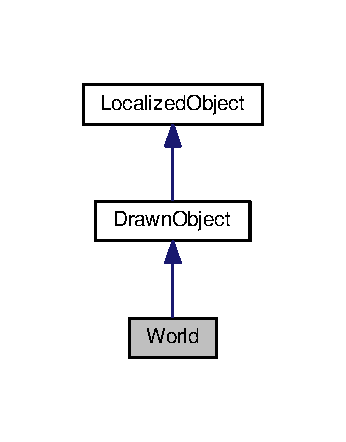
\includegraphics[width=166pt]{classWorld__inherit__graph}
\end{center}
\end{figure}


Collaboration diagram for World\+:\nopagebreak
\begin{figure}[H]
\begin{center}
\leavevmode
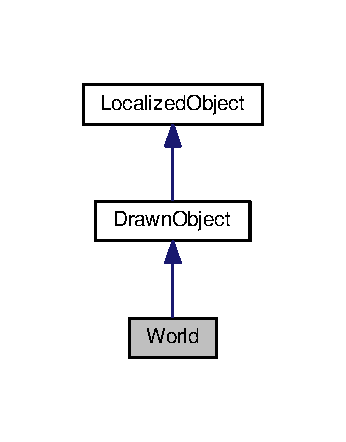
\includegraphics[width=166pt]{classWorld__coll__graph}
\end{center}
\end{figure}
\subsection*{Public Member Functions}
\begin{DoxyCompactItemize}
\item 
\hyperlink{classWorld_ae8ea8ff0609d5b37530b0a4adae065a7}{World} (double \hyperlink{classWorld_acbccb3a895843e63ed03d9a7f0ba04cf}{width}, double \hyperlink{classWorld_a5e0272d13155839a79169c4fddd2f9a4}{height}, int \hyperlink{classWorld_aa2de6ef451e67aac4bf028923083cd62}{width\+View}, int \hyperlink{classWorld_ae39d4731ecb9e398b60e410e137f860e}{height\+View}, Vector3d \hyperlink{classLocalizedObject_a340834deefc9e5c39da1f26c4ebf4f8c}{position}=Vector3d(), double \hyperlink{classLocalizedObject_aa5f7b070b6dc97a64a90797a0bca56e2}{theta}=0)
\begin{DoxyCompactList}\small\item\em Constructor. \end{DoxyCompactList}\item 
virtual \hyperlink{classWorld_a8c73fba541a5817fff65147ba47cd827}{$\sim$\+World} ()
\begin{DoxyCompactList}\small\item\em Destructor. \end{DoxyCompactList}\item 
double \hyperlink{classWorld_acc2f99cc48ee603c645c5fbd55762bb6}{get\+Height} () const 
\begin{DoxyCompactList}\small\item\em Simple getter. \end{DoxyCompactList}\item 
void \hyperlink{classWorld_a5d4ac723e964c5957f1bbd9e412e9bbe}{set\+Height} (double \hyperlink{classWorld_a5e0272d13155839a79169c4fddd2f9a4}{height})
\begin{DoxyCompactList}\small\item\em Simple setter. \end{DoxyCompactList}\item 
double \hyperlink{classWorld_ace9245fcf22b906eb1dd1e18e823d9cd}{get\+Height\+View} () const 
\begin{DoxyCompactList}\small\item\em Simple getter. \end{DoxyCompactList}\item 
void \hyperlink{classWorld_ab827fe0d14a6f60fe18e2ed5ee92d328}{set\+Height\+View} (double \hyperlink{classWorld_ae39d4731ecb9e398b60e410e137f860e}{height\+View})
\begin{DoxyCompactList}\small\item\em Simple setter. \end{DoxyCompactList}\item 
double \hyperlink{classWorld_ac5671c60bf3032e7786cb4a4b783ac03}{get\+Width} () const 
\begin{DoxyCompactList}\small\item\em Simple getter. \end{DoxyCompactList}\item 
void \hyperlink{classWorld_ae940c3db7c69cef5ab40547b20bd8747}{set\+Width} (double \hyperlink{classWorld_acbccb3a895843e63ed03d9a7f0ba04cf}{width})
\begin{DoxyCompactList}\small\item\em Simple setter. \end{DoxyCompactList}\item 
double \hyperlink{classWorld_a0c9a4b4d7430fc661d2c59ca001bcbfc}{get\+Width\+View} () const 
\begin{DoxyCompactList}\small\item\em Simple getter. \end{DoxyCompactList}\item 
void \hyperlink{classWorld_aa62c42795f5f1508491e5a3d9147c8e3}{set\+Width\+View} (double \hyperlink{classWorld_aa2de6ef451e67aac4bf028923083cd62}{width\+View})
\begin{DoxyCompactList}\small\item\em Simple setter. \end{DoxyCompactList}\end{DoxyCompactItemize}
\subsection*{Public Attributes}
\begin{DoxyCompactItemize}
\item 
double \hyperlink{classWorld_acbccb3a895843e63ed03d9a7f0ba04cf}{width}\hypertarget{classWorld_acbccb3a895843e63ed03d9a7f0ba04cf}{}\label{classWorld_acbccb3a895843e63ed03d9a7f0ba04cf}

\begin{DoxyCompactList}\small\item\em The real width of the \hyperlink{classWorld}{World} in meter. \end{DoxyCompactList}\item 
double \hyperlink{classWorld_a5e0272d13155839a79169c4fddd2f9a4}{height}\hypertarget{classWorld_a5e0272d13155839a79169c4fddd2f9a4}{}\label{classWorld_a5e0272d13155839a79169c4fddd2f9a4}

\begin{DoxyCompactList}\small\item\em The real height of the \hyperlink{classWorld}{World} in meter. \end{DoxyCompactList}\item 
double \hyperlink{classWorld_aa2de6ef451e67aac4bf028923083cd62}{width\+View}\hypertarget{classWorld_aa2de6ef451e67aac4bf028923083cd62}{}\label{classWorld_aa2de6ef451e67aac4bf028923083cd62}

\begin{DoxyCompactList}\small\item\em The projection width of the \hyperlink{classWorld}{World} in pixel. \end{DoxyCompactList}\item 
double \hyperlink{classWorld_ae39d4731ecb9e398b60e410e137f860e}{height\+View}\hypertarget{classWorld_ae39d4731ecb9e398b60e410e137f860e}{}\label{classWorld_ae39d4731ecb9e398b60e410e137f860e}

\begin{DoxyCompactList}\small\item\em The projection height of the \hyperlink{classWorld}{World} in pixel. \end{DoxyCompactList}\end{DoxyCompactItemize}
\subsection*{Additional Inherited Members}


\subsection{Detailed Description}
This class represent the main frame coordinates and its projection in pixels. 

\subsection{Constructor \& Destructor Documentation}
\index{World@{World}!World@{World}}
\index{World@{World}!World@{World}}
\subsubsection[{\texorpdfstring{World(double width, double height, int width\+View, int height\+View, Vector3d position=\+Vector3d(), double theta=0)}{World(double width, double height, int widthView, int heightView, Vector3d position=Vector3d(), double theta=0)}}]{\setlength{\rightskip}{0pt plus 5cm}World\+::\+World (
\begin{DoxyParamCaption}
\item[{double}]{width, }
\item[{double}]{height, }
\item[{int}]{width\+View, }
\item[{int}]{height\+View, }
\item[{Vector3d}]{position = {\ttfamily Vector3d()}, }
\item[{double}]{theta = {\ttfamily 0}}
\end{DoxyParamCaption}
)}\hypertarget{classWorld_ae8ea8ff0609d5b37530b0a4adae065a7}{}\label{classWorld_ae8ea8ff0609d5b37530b0a4adae065a7}


Constructor. 

Constructor of the \hyperlink{classWorld}{World} class


\begin{DoxyParams}{Parameters}
{\em width} & \+: The real width of the \hyperlink{classWorld}{World} in meter \\
\hline
{\em height} & \+: The real height of the \hyperlink{classWorld}{World} in meter \\
\hline
{\em width\+View} & \+: The projection width of the \hyperlink{classWorld}{World} in pixel \\
\hline
{\em height\+View} & \+: The projection height of the \hyperlink{classWorld}{World} in pixel \\
\hline
{\em position} & \+: The position of the \hyperlink{classWorld}{World} in the G\+UI in pixel \\
\hline
{\em theta} & \+: The rotation of the \hyperlink{classWorld}{World} in the G\+UI in radian \\
\hline
\end{DoxyParams}
\index{World@{World}!````~World@{$\sim$\+World}}
\index{````~World@{$\sim$\+World}!World@{World}}
\subsubsection[{\texorpdfstring{$\sim$\+World()}{~World()}}]{\setlength{\rightskip}{0pt plus 5cm}World\+::$\sim$\+World (
\begin{DoxyParamCaption}
{}
\end{DoxyParamCaption}
)\hspace{0.3cm}{\ttfamily [virtual]}}\hypertarget{classWorld_a8c73fba541a5817fff65147ba47cd827}{}\label{classWorld_a8c73fba541a5817fff65147ba47cd827}


Destructor. 

Destructor of the \hyperlink{classWorld}{World} class 

\subsection{Member Function Documentation}
\index{World@{World}!get\+Height@{get\+Height}}
\index{get\+Height@{get\+Height}!World@{World}}
\subsubsection[{\texorpdfstring{get\+Height() const }{getHeight() const }}]{\setlength{\rightskip}{0pt plus 5cm}double World\+::get\+Height (
\begin{DoxyParamCaption}
{}
\end{DoxyParamCaption}
) const}\hypertarget{classWorld_acc2f99cc48ee603c645c5fbd55762bb6}{}\label{classWorld_acc2f99cc48ee603c645c5fbd55762bb6}


Simple getter. 

\begin{DoxyReturn}{Returns}
height 
\end{DoxyReturn}
\index{World@{World}!get\+Height\+View@{get\+Height\+View}}
\index{get\+Height\+View@{get\+Height\+View}!World@{World}}
\subsubsection[{\texorpdfstring{get\+Height\+View() const }{getHeightView() const }}]{\setlength{\rightskip}{0pt plus 5cm}double World\+::get\+Height\+View (
\begin{DoxyParamCaption}
{}
\end{DoxyParamCaption}
) const}\hypertarget{classWorld_ace9245fcf22b906eb1dd1e18e823d9cd}{}\label{classWorld_ace9245fcf22b906eb1dd1e18e823d9cd}


Simple getter. 

\begin{DoxyReturn}{Returns}
height\+View 
\end{DoxyReturn}
\index{World@{World}!get\+Width@{get\+Width}}
\index{get\+Width@{get\+Width}!World@{World}}
\subsubsection[{\texorpdfstring{get\+Width() const }{getWidth() const }}]{\setlength{\rightskip}{0pt plus 5cm}double World\+::get\+Width (
\begin{DoxyParamCaption}
{}
\end{DoxyParamCaption}
) const}\hypertarget{classWorld_ac5671c60bf3032e7786cb4a4b783ac03}{}\label{classWorld_ac5671c60bf3032e7786cb4a4b783ac03}


Simple getter. 

\begin{DoxyReturn}{Returns}
width 
\end{DoxyReturn}
\index{World@{World}!get\+Width\+View@{get\+Width\+View}}
\index{get\+Width\+View@{get\+Width\+View}!World@{World}}
\subsubsection[{\texorpdfstring{get\+Width\+View() const }{getWidthView() const }}]{\setlength{\rightskip}{0pt plus 5cm}double World\+::get\+Width\+View (
\begin{DoxyParamCaption}
{}
\end{DoxyParamCaption}
) const}\hypertarget{classWorld_a0c9a4b4d7430fc661d2c59ca001bcbfc}{}\label{classWorld_a0c9a4b4d7430fc661d2c59ca001bcbfc}


Simple getter. 

\begin{DoxyReturn}{Returns}
width\+View 
\end{DoxyReturn}
\index{World@{World}!set\+Height@{set\+Height}}
\index{set\+Height@{set\+Height}!World@{World}}
\subsubsection[{\texorpdfstring{set\+Height(double height)}{setHeight(double height)}}]{\setlength{\rightskip}{0pt plus 5cm}void World\+::set\+Height (
\begin{DoxyParamCaption}
\item[{double}]{height}
\end{DoxyParamCaption}
)}\hypertarget{classWorld_a5d4ac723e964c5957f1bbd9e412e9bbe}{}\label{classWorld_a5d4ac723e964c5957f1bbd9e412e9bbe}


Simple setter. 


\begin{DoxyParams}{Parameters}
{\em height} & \\
\hline
\end{DoxyParams}
\index{World@{World}!set\+Height\+View@{set\+Height\+View}}
\index{set\+Height\+View@{set\+Height\+View}!World@{World}}
\subsubsection[{\texorpdfstring{set\+Height\+View(double height\+View)}{setHeightView(double heightView)}}]{\setlength{\rightskip}{0pt plus 5cm}void World\+::set\+Height\+View (
\begin{DoxyParamCaption}
\item[{double}]{height\+View}
\end{DoxyParamCaption}
)}\hypertarget{classWorld_ab827fe0d14a6f60fe18e2ed5ee92d328}{}\label{classWorld_ab827fe0d14a6f60fe18e2ed5ee92d328}


Simple setter. 


\begin{DoxyParams}{Parameters}
{\em height\+View} & \\
\hline
\end{DoxyParams}
\index{World@{World}!set\+Width@{set\+Width}}
\index{set\+Width@{set\+Width}!World@{World}}
\subsubsection[{\texorpdfstring{set\+Width(double width)}{setWidth(double width)}}]{\setlength{\rightskip}{0pt plus 5cm}void World\+::set\+Width (
\begin{DoxyParamCaption}
\item[{double}]{width}
\end{DoxyParamCaption}
)}\hypertarget{classWorld_ae940c3db7c69cef5ab40547b20bd8747}{}\label{classWorld_ae940c3db7c69cef5ab40547b20bd8747}


Simple setter. 


\begin{DoxyParams}{Parameters}
{\em width} & \\
\hline
\end{DoxyParams}
\index{World@{World}!set\+Width\+View@{set\+Width\+View}}
\index{set\+Width\+View@{set\+Width\+View}!World@{World}}
\subsubsection[{\texorpdfstring{set\+Width\+View(double width\+View)}{setWidthView(double widthView)}}]{\setlength{\rightskip}{0pt plus 5cm}void World\+::set\+Width\+View (
\begin{DoxyParamCaption}
\item[{double}]{width\+View}
\end{DoxyParamCaption}
)}\hypertarget{classWorld_aa62c42795f5f1508491e5a3d9147c8e3}{}\label{classWorld_aa62c42795f5f1508491e5a3d9147c8e3}


Simple setter. 


\begin{DoxyParams}{Parameters}
{\em width\+View} & \\
\hline
\end{DoxyParams}


The documentation for this class was generated from the following files\+:\begin{DoxyCompactItemize}
\item 
src/world\+Representation/\hyperlink{World_8h}{World.\+h}\item 
src/world\+Representation/World.\+cpp\end{DoxyCompactItemize}

\chapter{File Documentation}
\hypertarget{Agent_8cpp}{}\section{src/agent\+Management/\+Agent.cpp File Reference}
\label{Agent_8cpp}\index{src/agent\+Management/\+Agent.\+cpp@{src/agent\+Management/\+Agent.\+cpp}}
{\ttfamily \#include \char`\"{}Agent.\+h\char`\"{}}\\*
{\ttfamily \#include \char`\"{}Gaussian\+Space.\+h\char`\"{}}\\*
{\ttfamily \#include \char`\"{}Formation.\+h\char`\"{}}\\*
{\ttfamily \#include $<$limits$>$}\\*
{\ttfamily \#include \char`\"{}utils.\+h\char`\"{}}\\*
Include dependency graph for Agent.\+cpp\+:\nopagebreak
\begin{figure}[H]
\begin{center}
\leavevmode
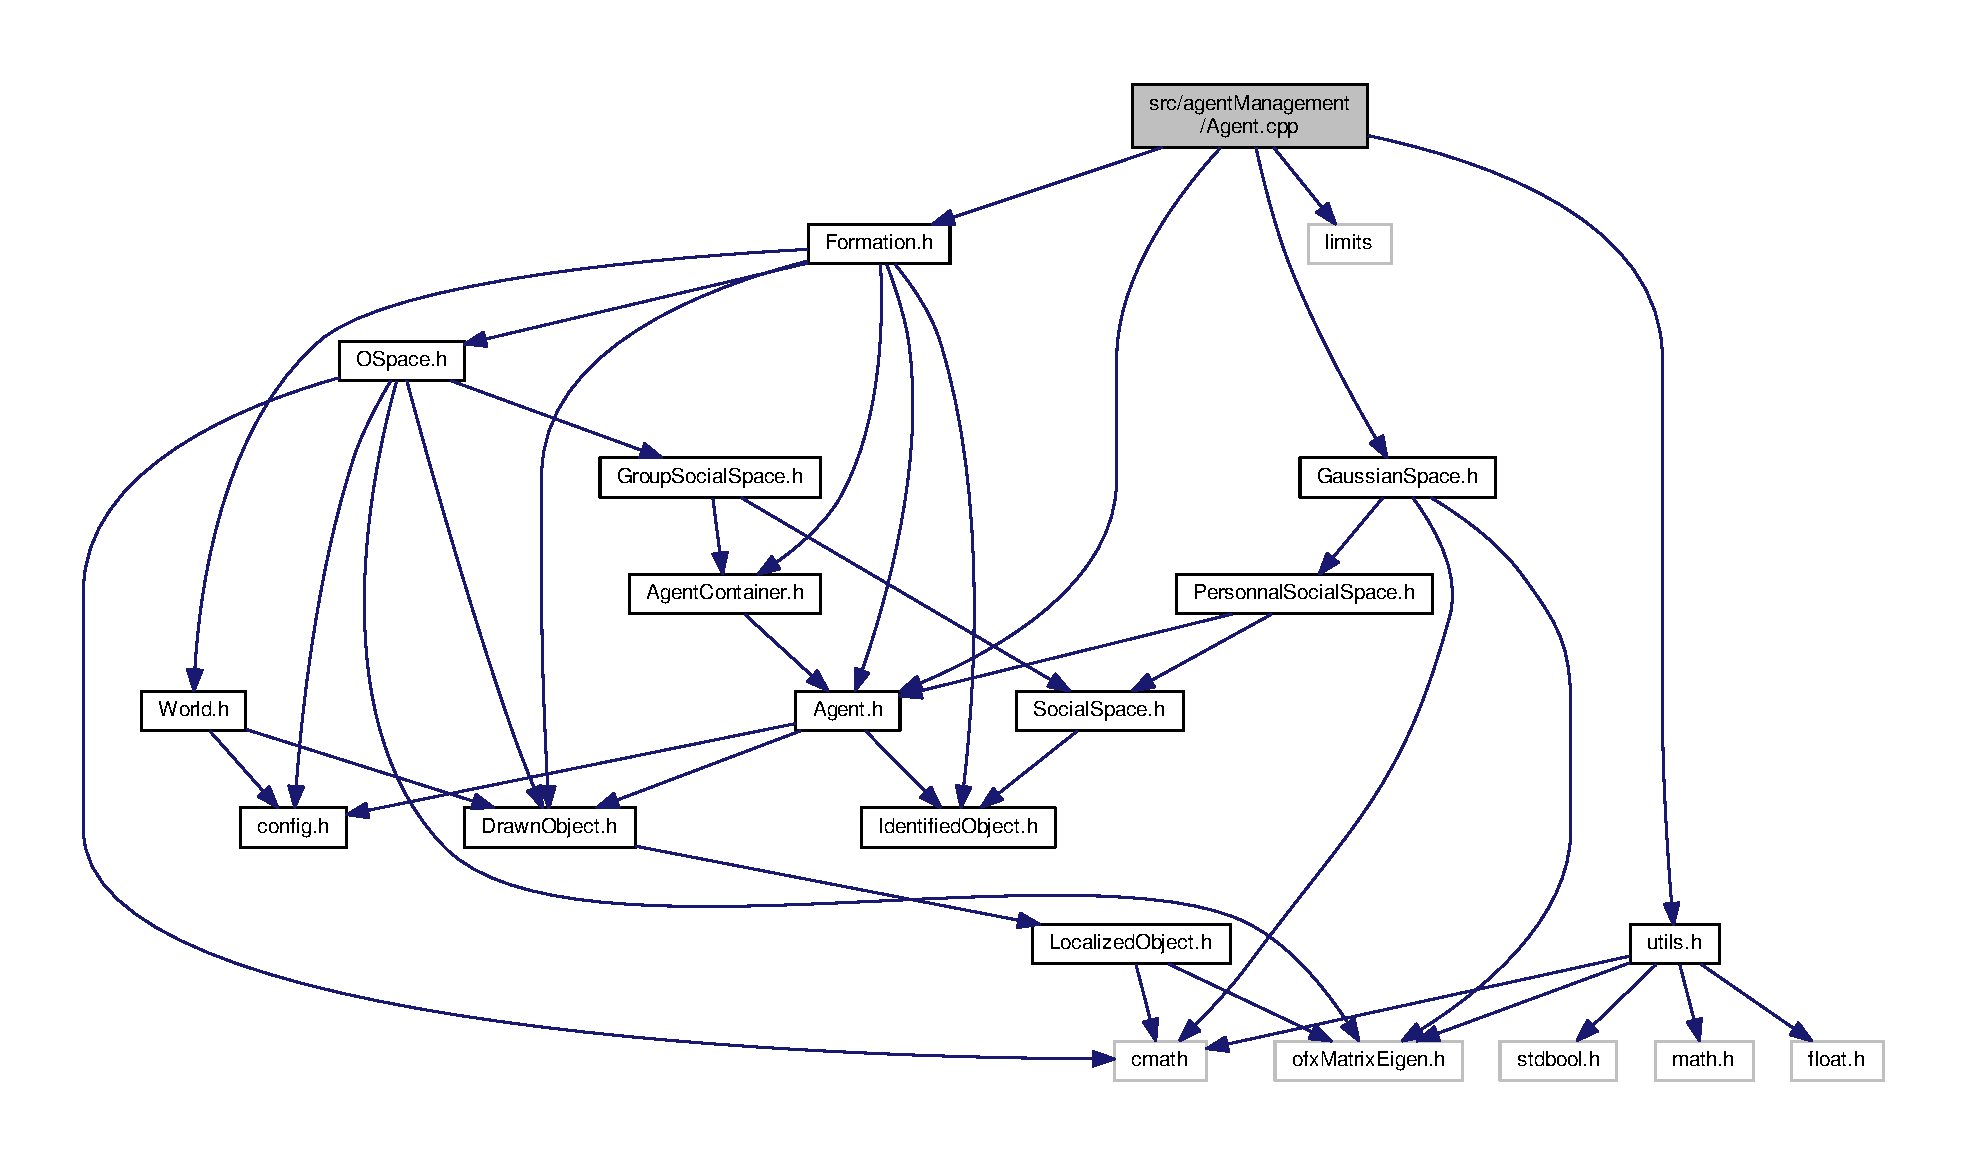
\includegraphics[width=350pt]{Agent_8cpp__incl}
\end{center}
\end{figure}


\subsection{Detailed Description}
\begin{DoxyAuthor}{Author}
Paco Dupont 
\end{DoxyAuthor}
\begin{DoxyVersion}{Version}
0.\+1 
\end{DoxyVersion}
\begin{DoxyDate}{Date}
24 mars 2017 
\end{DoxyDate}

\hypertarget{Agent_8h}{}\section{src/agent\+Management/\+Agent.h File Reference}
\label{Agent_8h}\index{src/agent\+Management/\+Agent.\+h@{src/agent\+Management/\+Agent.\+h}}
{\ttfamily \#include \char`\"{}Identified\+Object.\+h\char`\"{}}\\*
{\ttfamily \#include \char`\"{}Drawn\+Object.\+h\char`\"{}}\\*
{\ttfamily \#include \char`\"{}config.\+h\char`\"{}}\\*
Include dependency graph for Agent.\+h\+:\nopagebreak
\begin{figure}[H]
\begin{center}
\leavevmode
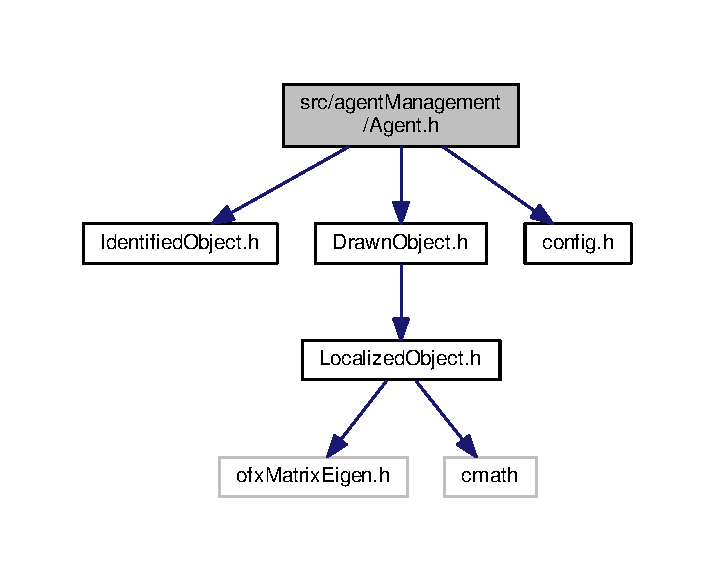
\includegraphics[width=343pt]{Agent_8h__incl}
\end{center}
\end{figure}
This graph shows which files directly or indirectly include this file\+:\nopagebreak
\begin{figure}[H]
\begin{center}
\leavevmode
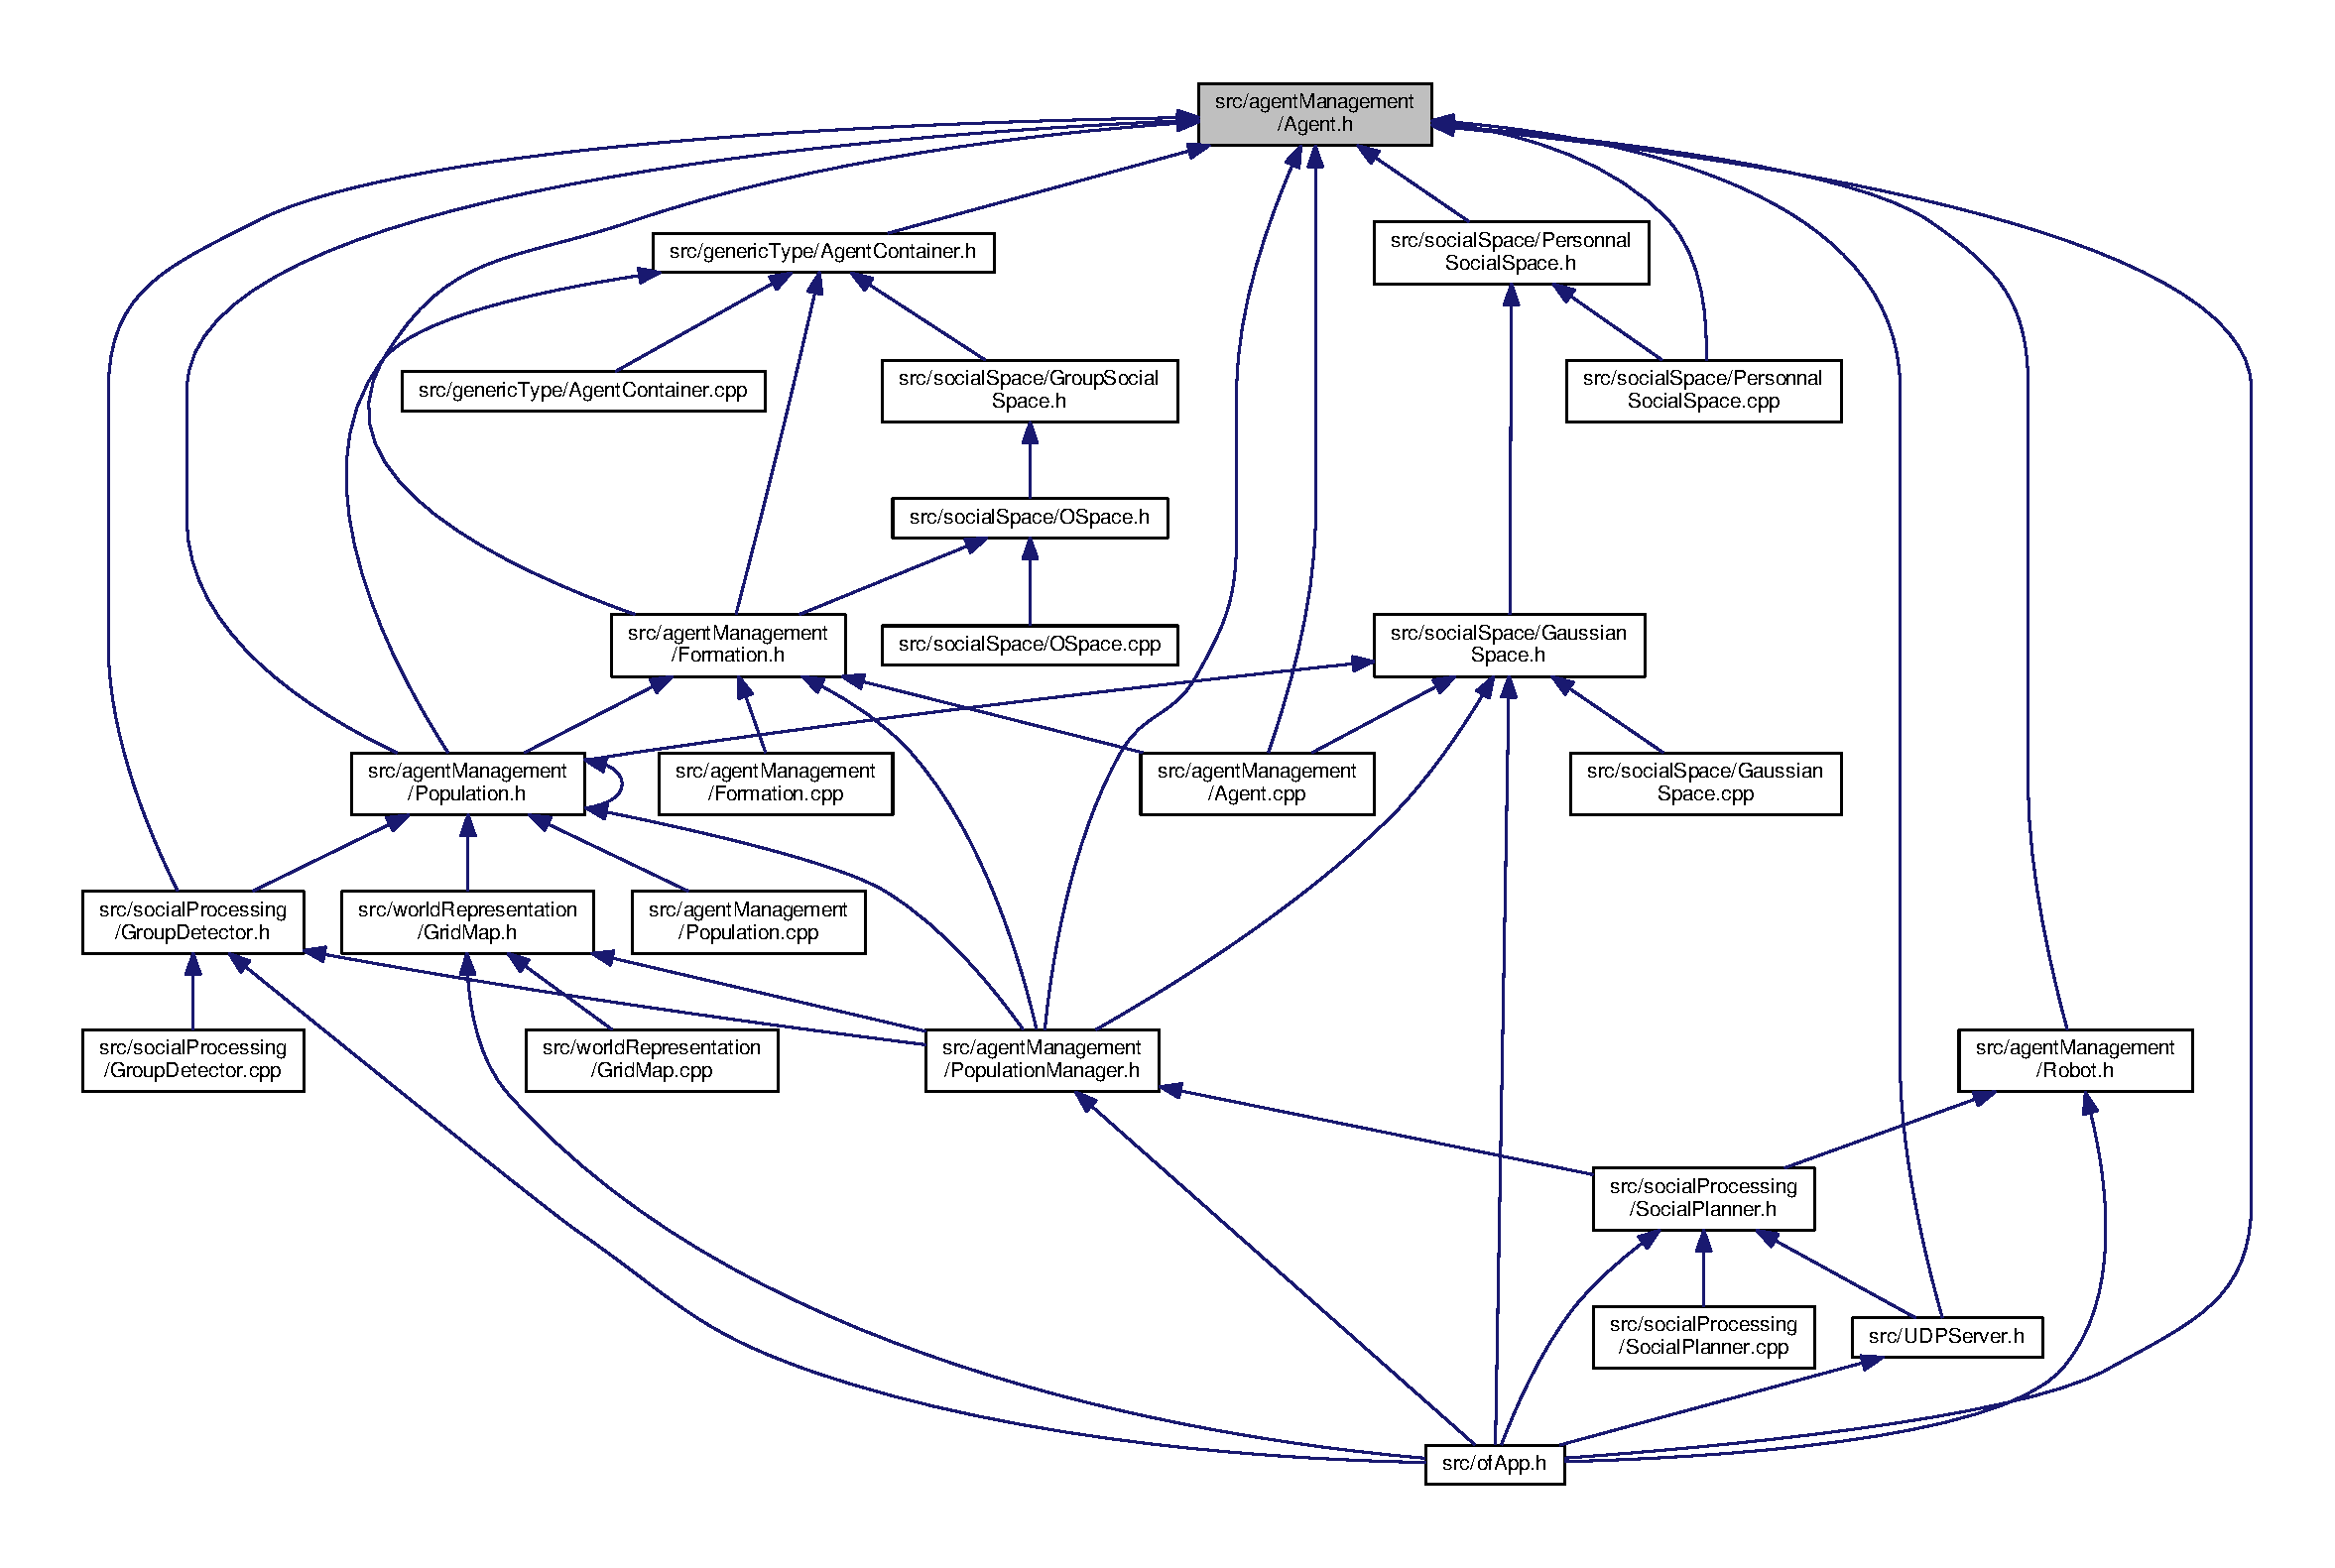
\includegraphics[width=350pt]{Agent_8h__dep__incl}
\end{center}
\end{figure}
\subsection*{Classes}
\begin{DoxyCompactItemize}
\item 
class \hyperlink{classAgent}{Agent}
\begin{DoxyCompactList}\small\item\em This class represent the Agents. \end{DoxyCompactList}\end{DoxyCompactItemize}


\subsection{Detailed Description}
\begin{DoxyAuthor}{Author}
Paco Dupont 
\end{DoxyAuthor}
\begin{DoxyVersion}{Version}
0.\+1 
\end{DoxyVersion}
\begin{DoxyDate}{Date}
24 mars 2017 
\end{DoxyDate}

\hypertarget{Formation_8cpp}{}\section{src/agent\+Management/\+Formation.cpp File Reference}
\label{Formation_8cpp}\index{src/agent\+Management/\+Formation.\+cpp@{src/agent\+Management/\+Formation.\+cpp}}
{\ttfamily \#include \char`\"{}Formation.\+h\char`\"{}}\\*
{\ttfamily \#include \char`\"{}config.\+h\char`\"{}}\\*
{\ttfamily \#include \char`\"{}utils.\+h\char`\"{}}\\*
Include dependency graph for Formation.\+cpp\+:\nopagebreak
\begin{figure}[H]
\begin{center}
\leavevmode
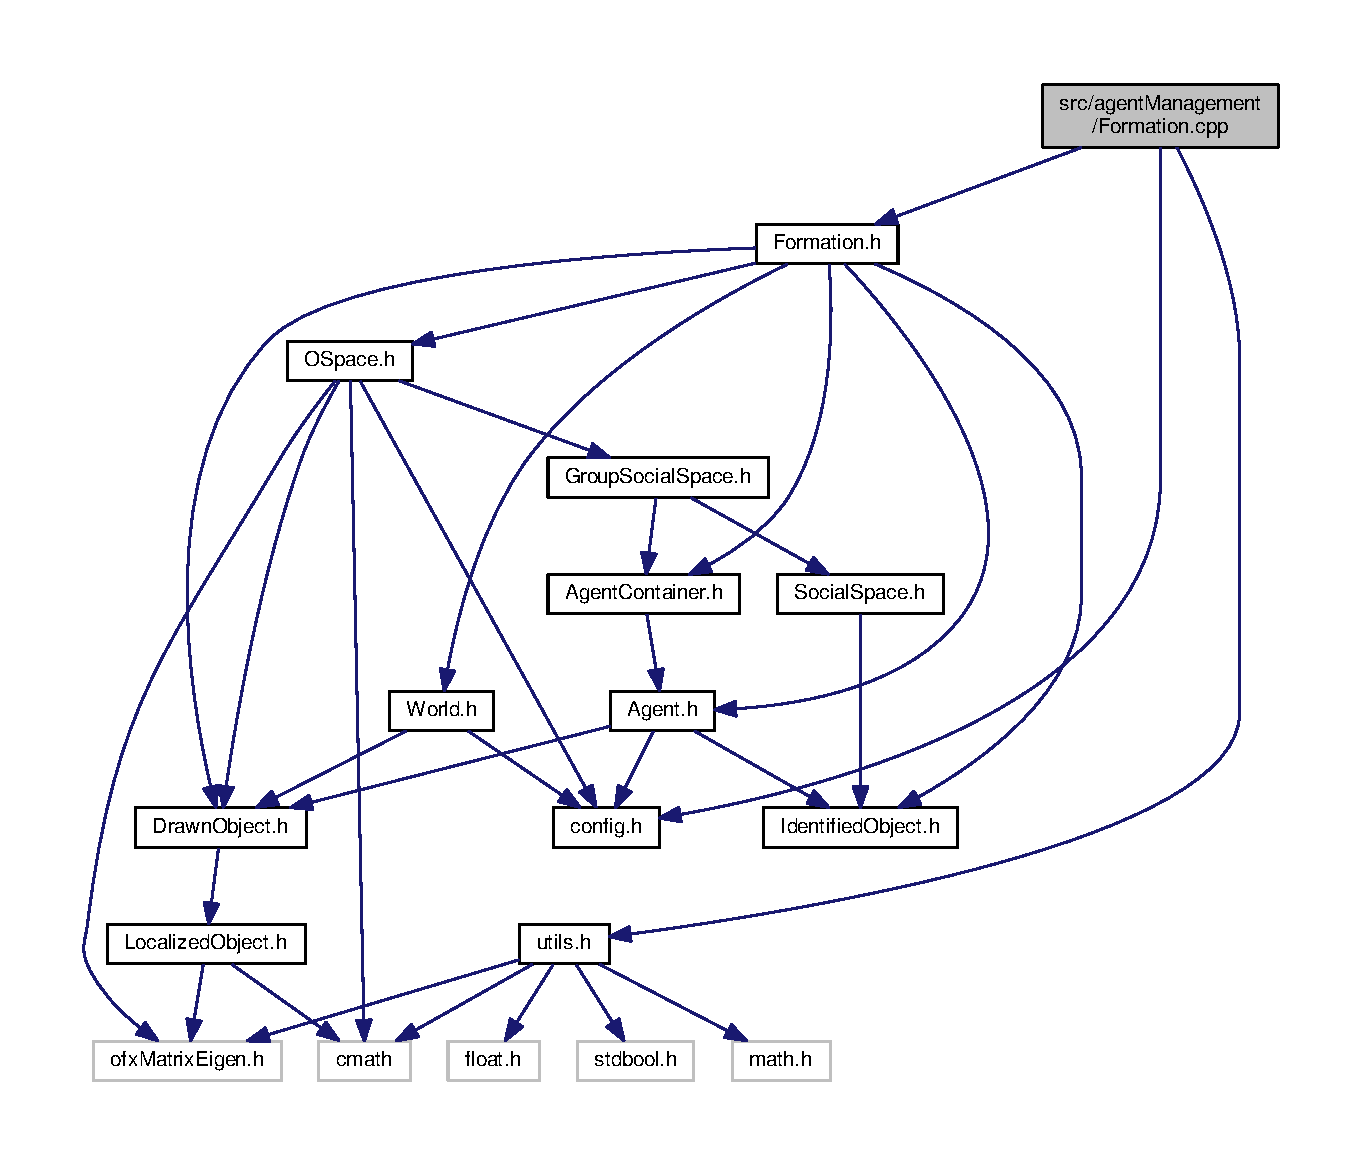
\includegraphics[width=350pt]{Formation_8cpp__incl}
\end{center}
\end{figure}


\subsection{Detailed Description}
\begin{DoxyAuthor}{Author}
Paco Dupont 
\end{DoxyAuthor}
\begin{DoxyVersion}{Version}
0.\+1 
\end{DoxyVersion}
\begin{DoxyDate}{Date}
24 mars 2017 
\end{DoxyDate}

\hypertarget{Formation_8h}{}\section{src/agent\+Management/\+Formation.h File Reference}
\label{Formation_8h}\index{src/agent\+Management/\+Formation.\+h@{src/agent\+Management/\+Formation.\+h}}
{\ttfamily \#include \char`\"{}Agent.\+h\char`\"{}}\\*
{\ttfamily \#include \char`\"{}Identified\+Object.\+h\char`\"{}}\\*
{\ttfamily \#include \char`\"{}Drawn\+Object.\+h\char`\"{}}\\*
{\ttfamily \#include \char`\"{}Agent\+Container.\+h\char`\"{}}\\*
{\ttfamily \#include \char`\"{}O\+Space.\+h\char`\"{}}\\*
{\ttfamily \#include \char`\"{}World.\+h\char`\"{}}\\*
Include dependency graph for Formation.\+h\+:\nopagebreak
\begin{figure}[H]
\begin{center}
\leavevmode
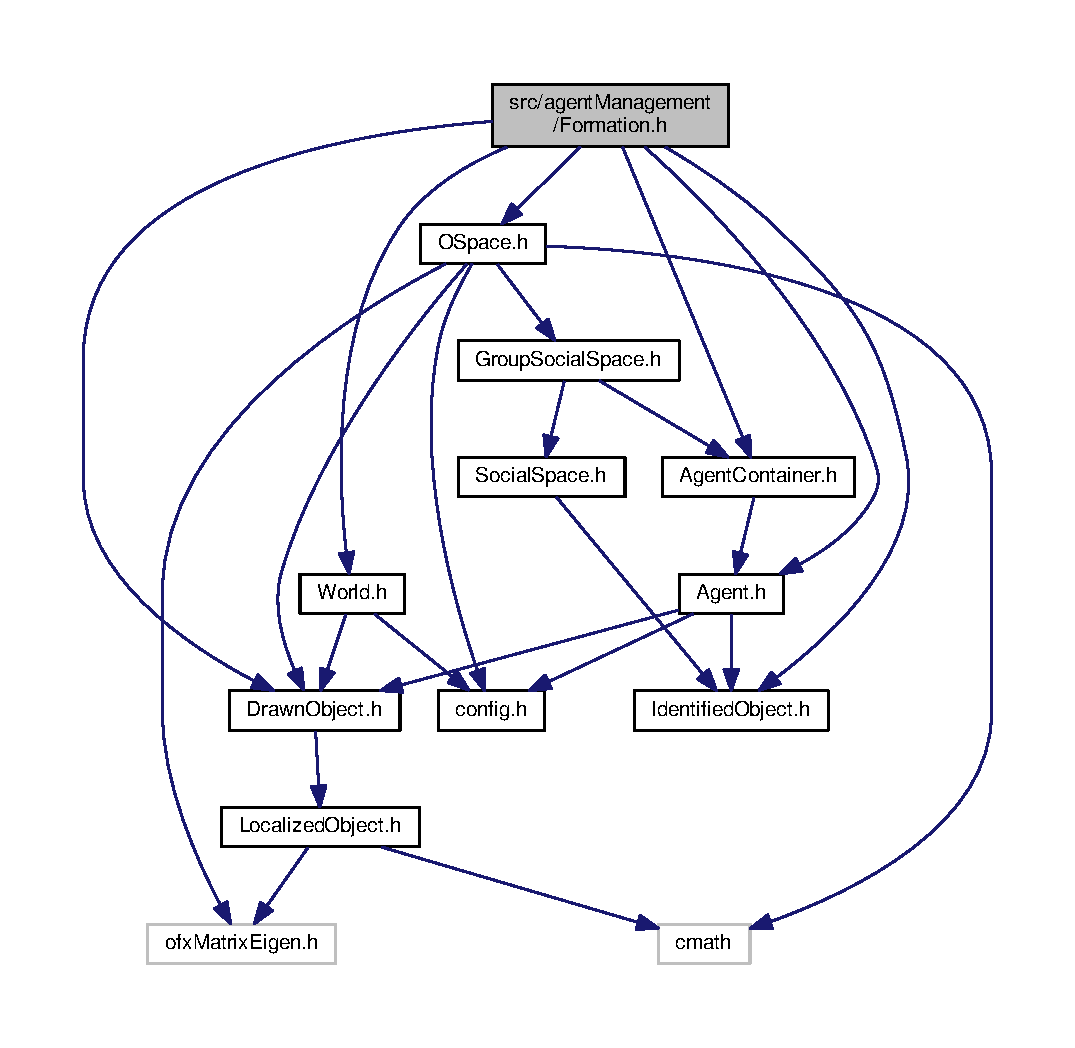
\includegraphics[width=350pt]{Formation_8h__incl}
\end{center}
\end{figure}
This graph shows which files directly or indirectly include this file\+:\nopagebreak
\begin{figure}[H]
\begin{center}
\leavevmode
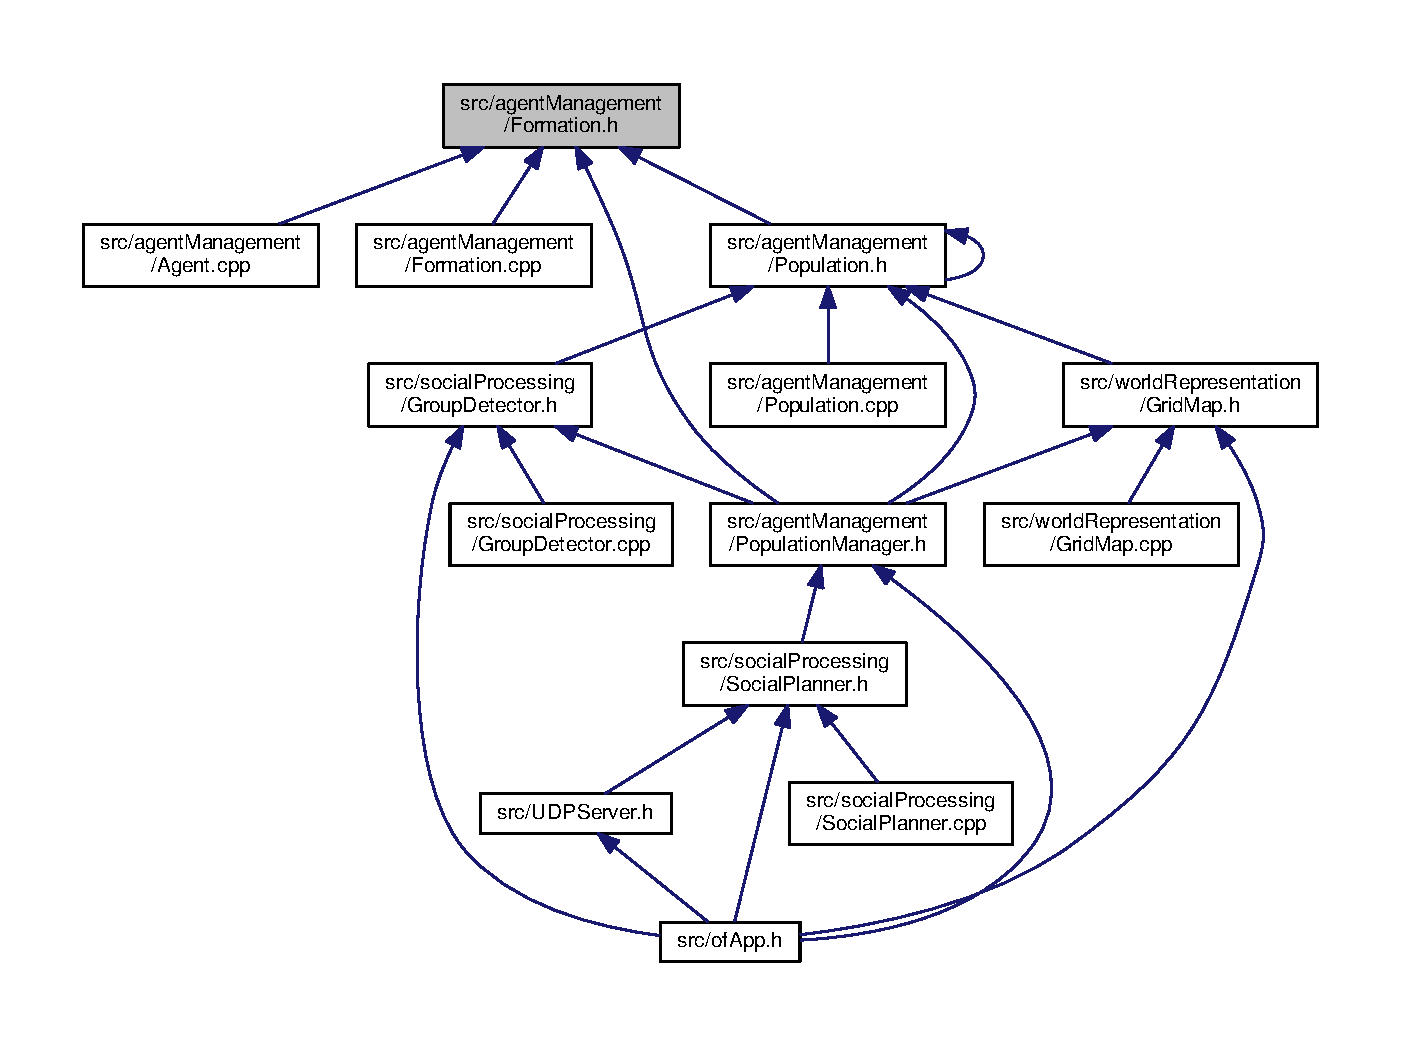
\includegraphics[width=350pt]{Formation_8h__dep__incl}
\end{center}
\end{figure}
\subsection*{Classes}
\begin{DoxyCompactItemize}
\item 
class \hyperlink{classFormation}{Formation}
\begin{DoxyCompactList}\small\item\em This class represent the social \hyperlink{classFormation}{Formation}. \end{DoxyCompactList}\end{DoxyCompactItemize}


\subsection{Detailed Description}
\begin{DoxyAuthor}{Author}
Paco Dupont 
\end{DoxyAuthor}
\begin{DoxyVersion}{Version}
0.\+1 
\end{DoxyVersion}
\begin{DoxyDate}{Date}
24 mars 2017 
\end{DoxyDate}

\hypertarget{Population_8cpp}{}\section{src/agent\+Management/\+Population.cpp File Reference}
\label{Population_8cpp}\index{src/agent\+Management/\+Population.\+cpp@{src/agent\+Management/\+Population.\+cpp}}
{\ttfamily \#include \char`\"{}Population.\+h\char`\"{}}\\*
Include dependency graph for Population.\+cpp\+:\nopagebreak
\begin{figure}[H]
\begin{center}
\leavevmode
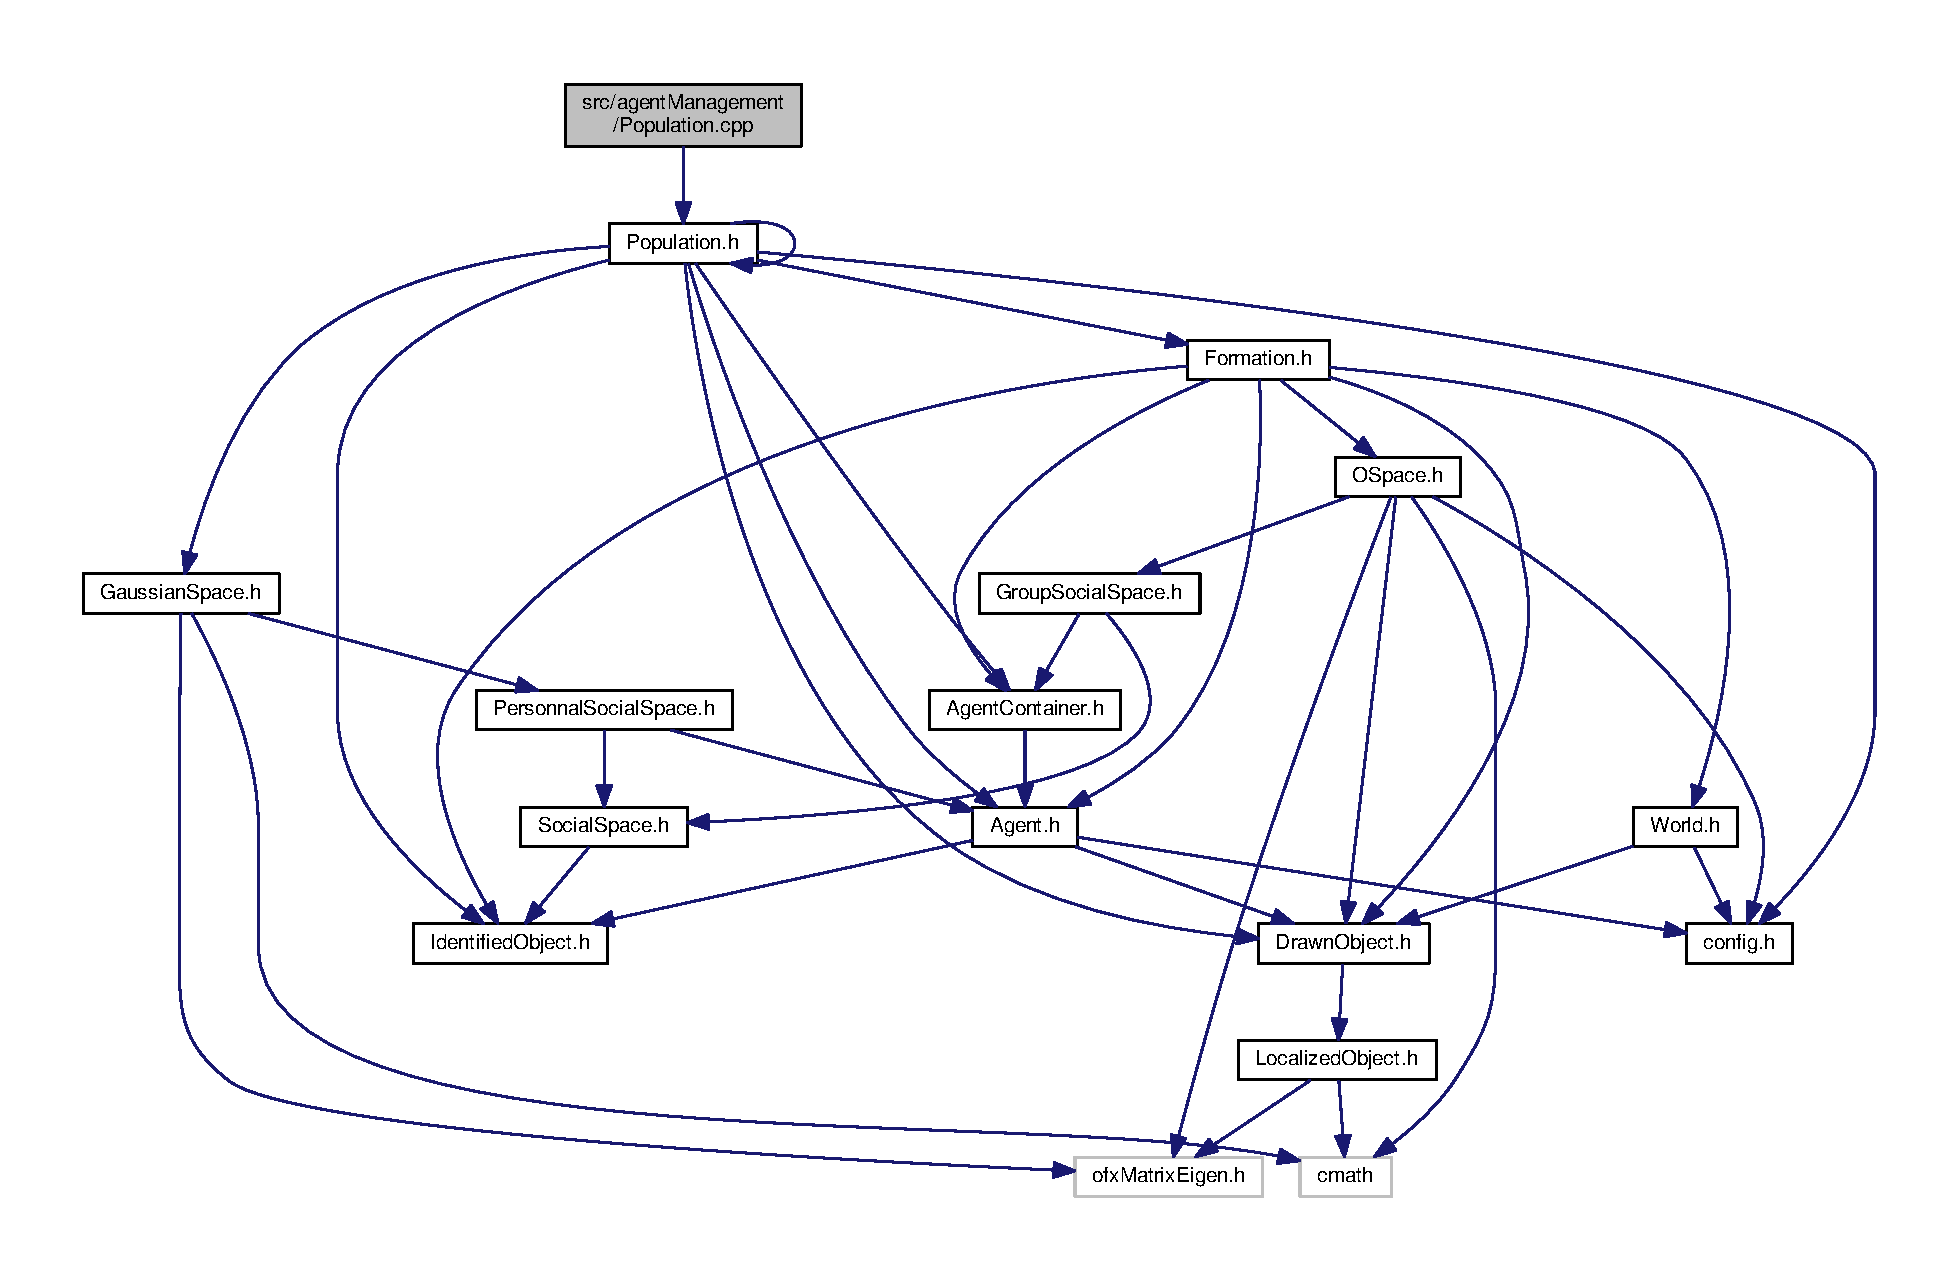
\includegraphics[width=350pt]{Population_8cpp__incl}
\end{center}
\end{figure}


\subsection{Detailed Description}
\begin{DoxyAuthor}{Author}
Paco Dupont 
\end{DoxyAuthor}
\begin{DoxyVersion}{Version}
0.\+1 
\end{DoxyVersion}
\begin{DoxyDate}{Date}
24 mars 2017 
\end{DoxyDate}

\hypertarget{Population_8h}{}\section{src/agent\+Management/\+Population.h File Reference}
\label{Population_8h}\index{src/agent\+Management/\+Population.\+h@{src/agent\+Management/\+Population.\+h}}
{\ttfamily \#include \char`\"{}Agent.\+h\char`\"{}}\\*
{\ttfamily \#include \char`\"{}Formation.\+h\char`\"{}}\\*
{\ttfamily \#include \char`\"{}Identified\+Object.\+h\char`\"{}}\\*
{\ttfamily \#include \char`\"{}Drawn\+Object.\+h\char`\"{}}\\*
{\ttfamily \#include \char`\"{}Agent\+Container.\+h\char`\"{}}\\*
{\ttfamily \#include \char`\"{}Population.\+h\char`\"{}}\\*
{\ttfamily \#include \char`\"{}Gaussian\+Space.\+h\char`\"{}}\\*
{\ttfamily \#include \char`\"{}config.\+h\char`\"{}}\\*
Include dependency graph for Population.\+h\+:\nopagebreak
\begin{figure}[H]
\begin{center}
\leavevmode
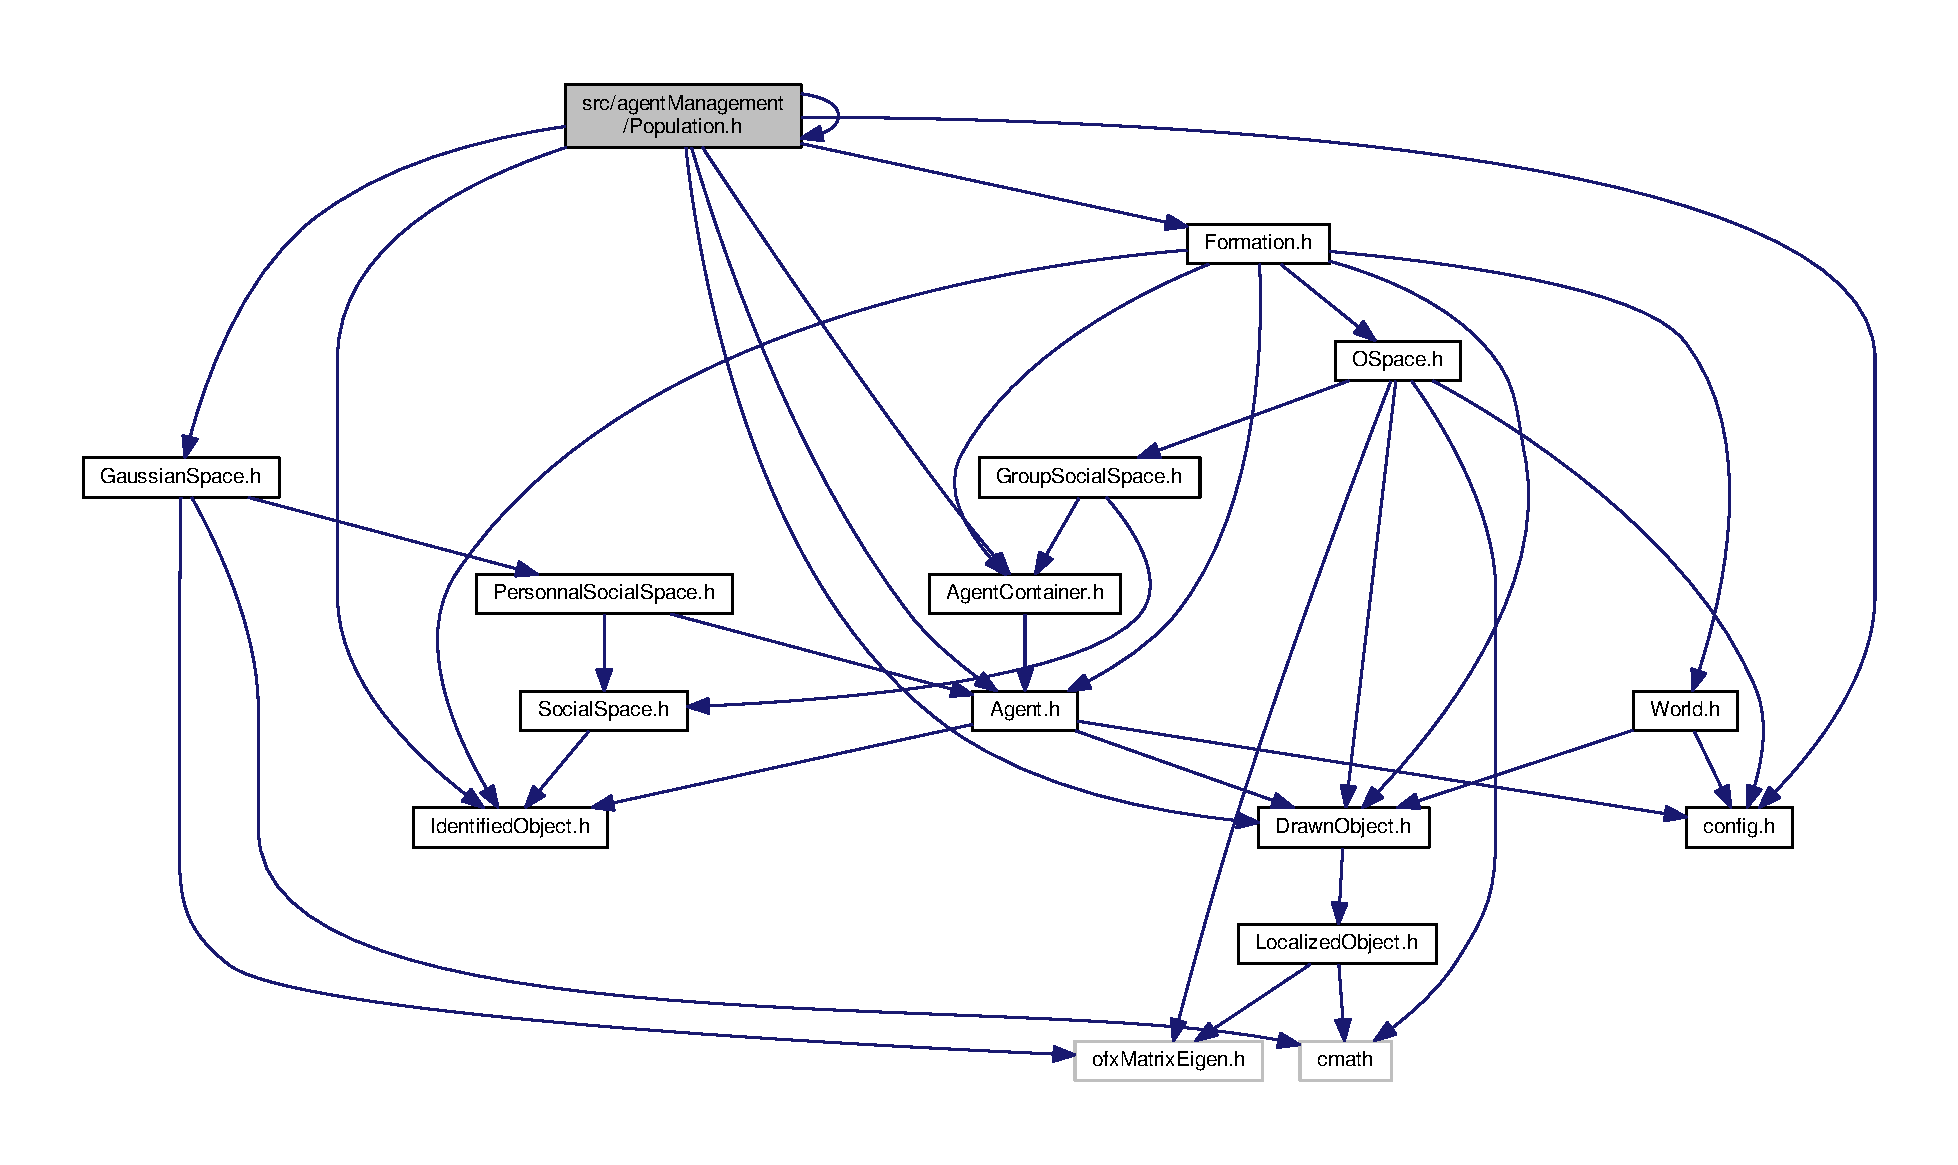
\includegraphics[width=350pt]{Population_8h__incl}
\end{center}
\end{figure}
This graph shows which files directly or indirectly include this file\+:\nopagebreak
\begin{figure}[H]
\begin{center}
\leavevmode
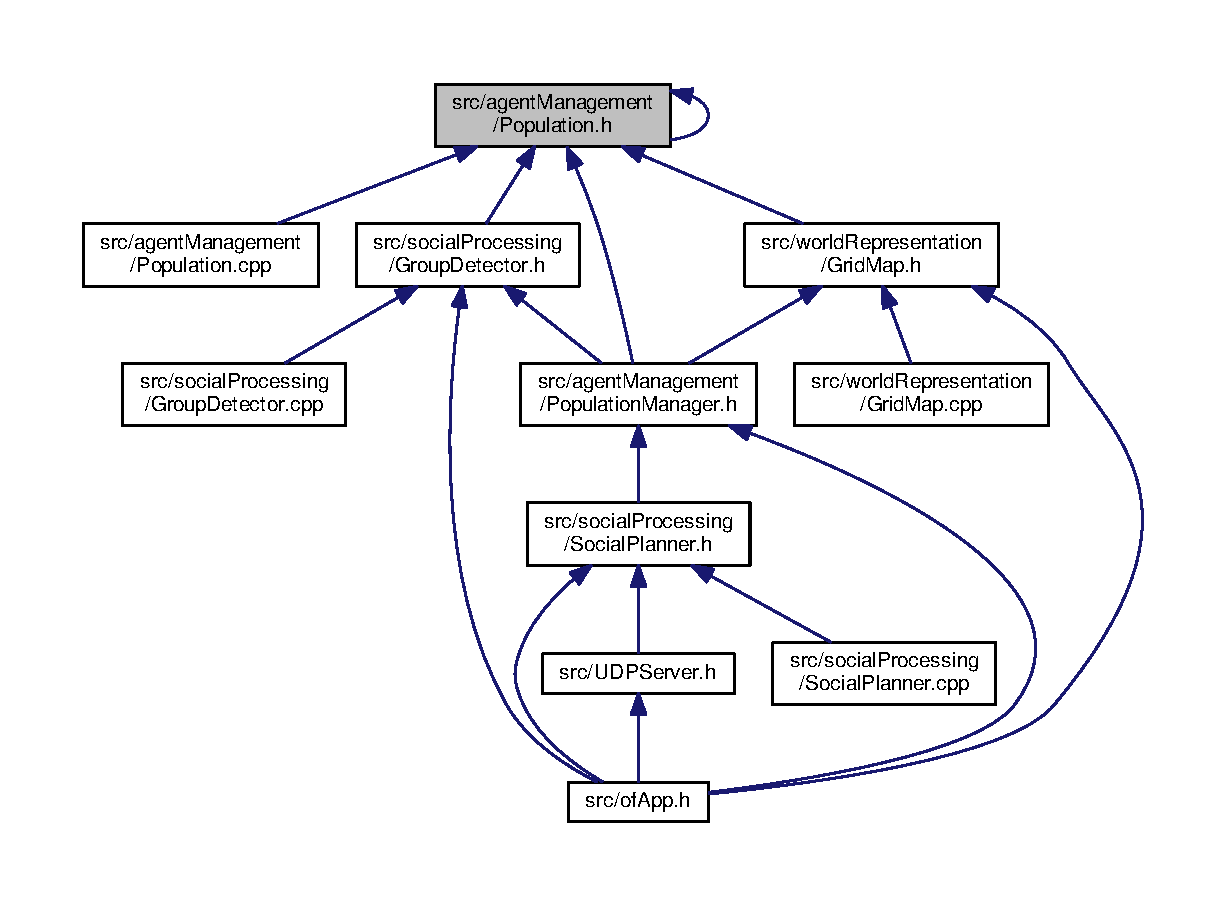
\includegraphics[width=350pt]{Population_8h__dep__incl}
\end{center}
\end{figure}
\subsection*{Classes}
\begin{DoxyCompactItemize}
\item 
class \hyperlink{classPopulation}{Population}
\begin{DoxyCompactList}\small\item\em This class represent \hyperlink{classPopulation}{Population} around the \hyperlink{classRobot}{Robot}. \end{DoxyCompactList}\end{DoxyCompactItemize}


\subsection{Detailed Description}
\begin{DoxyAuthor}{Author}
Paco Dupont 
\end{DoxyAuthor}
\begin{DoxyVersion}{Version}
0.\+1 
\end{DoxyVersion}
\begin{DoxyDate}{Date}
24 mars 2017 
\end{DoxyDate}

\hypertarget{Robot_8h}{}\section{src/agent\+Management/\+Robot.h File Reference}
\label{Robot_8h}\index{src/agent\+Management/\+Robot.\+h@{src/agent\+Management/\+Robot.\+h}}
{\ttfamily \#include \char`\"{}Identified\+Object.\+h\char`\"{}}\\*
{\ttfamily \#include \char`\"{}Drawn\+Object.\+h\char`\"{}}\\*
{\ttfamily \#include \char`\"{}World.\+h\char`\"{}}\\*
{\ttfamily \#include \char`\"{}Grid\+Cell.\+h\char`\"{}}\\*
{\ttfamily \#include \char`\"{}Agent.\+h\char`\"{}}\\*
{\ttfamily \#include $<$chrono$>$}\\*
Include dependency graph for Robot.\+h\+:\nopagebreak
\begin{figure}[H]
\begin{center}
\leavevmode
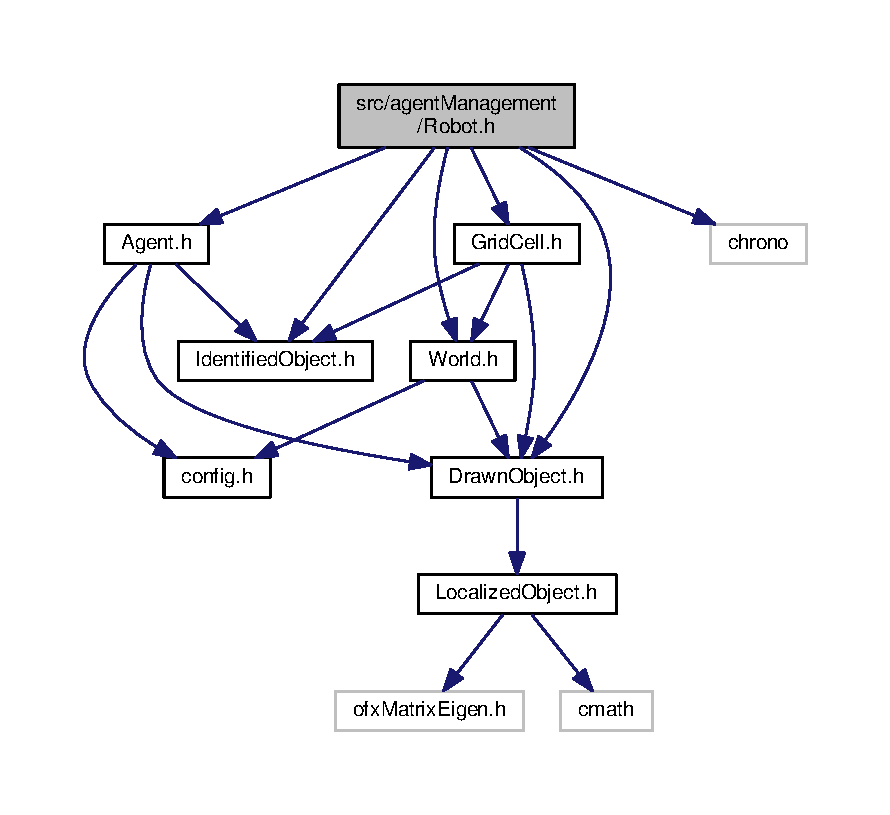
\includegraphics[width=350pt]{Robot_8h__incl}
\end{center}
\end{figure}
This graph shows which files directly or indirectly include this file\+:\nopagebreak
\begin{figure}[H]
\begin{center}
\leavevmode
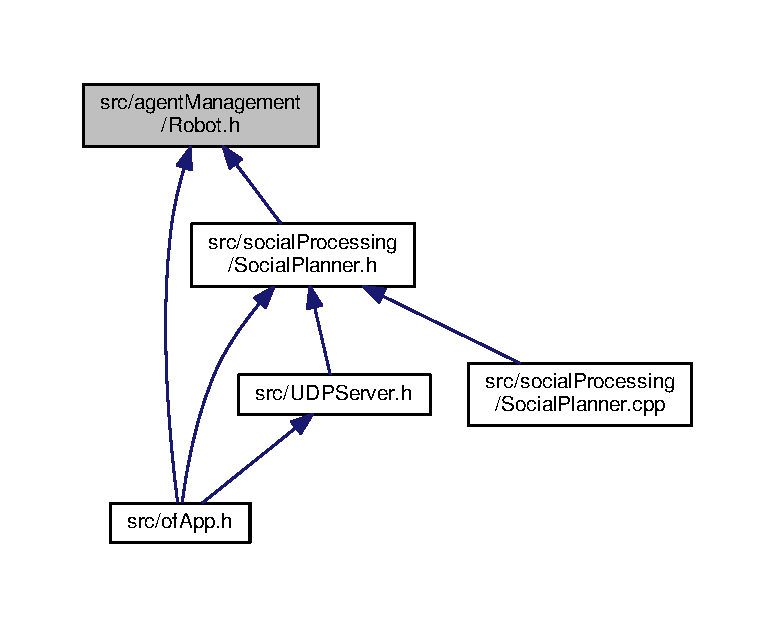
\includegraphics[width=350pt]{Robot_8h__dep__incl}
\end{center}
\end{figure}
\subsection*{Classes}
\begin{DoxyCompactItemize}
\item 
class \hyperlink{classRobot}{Robot}
\begin{DoxyCompactList}\small\item\em This class represent the \hyperlink{classRobot}{Robot}. \end{DoxyCompactList}\end{DoxyCompactItemize}


\subsection{Detailed Description}
\begin{DoxyAuthor}{Author}
Paco Dupont 
\end{DoxyAuthor}
\begin{DoxyVersion}{Version}
0.\+1 
\end{DoxyVersion}
\begin{DoxyDate}{Date}
7 juin 2017 
\end{DoxyDate}

\hypertarget{AgentContainer_8cpp}{}\section{src/generic\+Type/\+Agent\+Container.cpp File Reference}
\label{AgentContainer_8cpp}\index{src/generic\+Type/\+Agent\+Container.\+cpp@{src/generic\+Type/\+Agent\+Container.\+cpp}}
{\ttfamily \#include \char`\"{}Agent\+Container.\+h\char`\"{}}\\*
Include dependency graph for Agent\+Container.\+cpp\+:\nopagebreak
\begin{figure}[H]
\begin{center}
\leavevmode
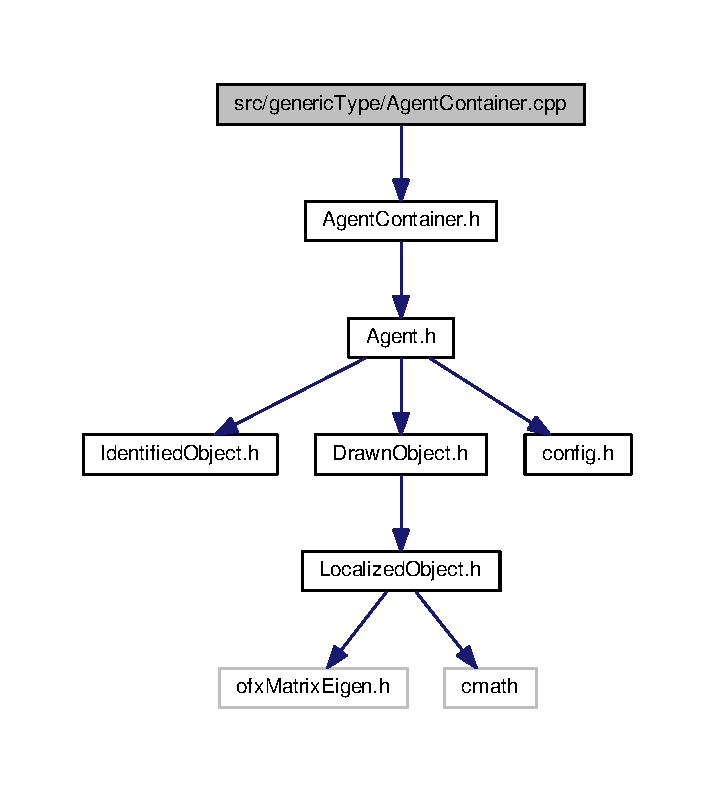
\includegraphics[width=343pt]{AgentContainer_8cpp__incl}
\end{center}
\end{figure}


\subsection{Detailed Description}
\begin{DoxyAuthor}{Author}
Paco Dupont 
\end{DoxyAuthor}
\begin{DoxyVersion}{Version}
0.\+1 
\end{DoxyVersion}
\begin{DoxyDate}{Date}
27 mars 2017 
\end{DoxyDate}

\hypertarget{AgentContainer_8h}{}\section{src/generic\+Type/\+Agent\+Container.h File Reference}
\label{AgentContainer_8h}\index{src/generic\+Type/\+Agent\+Container.\+h@{src/generic\+Type/\+Agent\+Container.\+h}}
{\ttfamily \#include \char`\"{}Agent.\+h\char`\"{}}\\*
Include dependency graph for Agent\+Container.\+h\+:\nopagebreak
\begin{figure}[H]
\begin{center}
\leavevmode
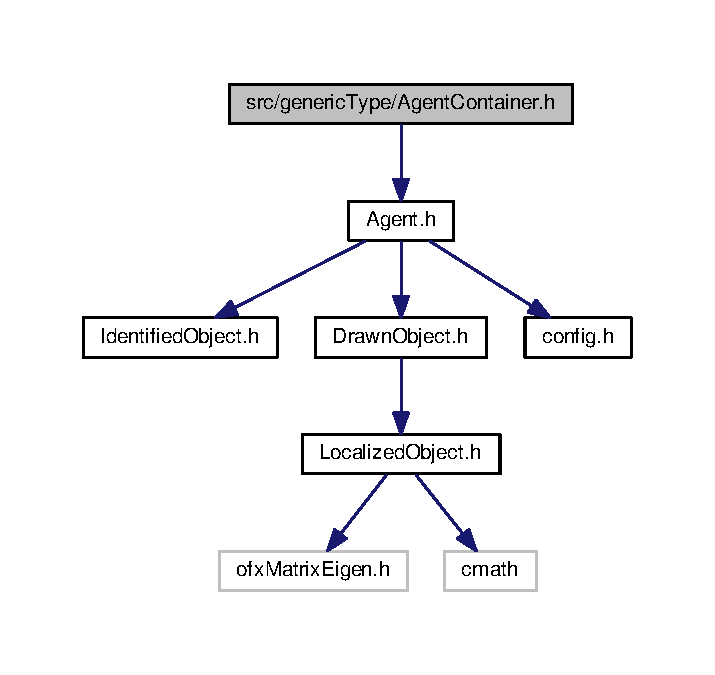
\includegraphics[width=343pt]{AgentContainer_8h__incl}
\end{center}
\end{figure}
This graph shows which files directly or indirectly include this file\+:\nopagebreak
\begin{figure}[H]
\begin{center}
\leavevmode
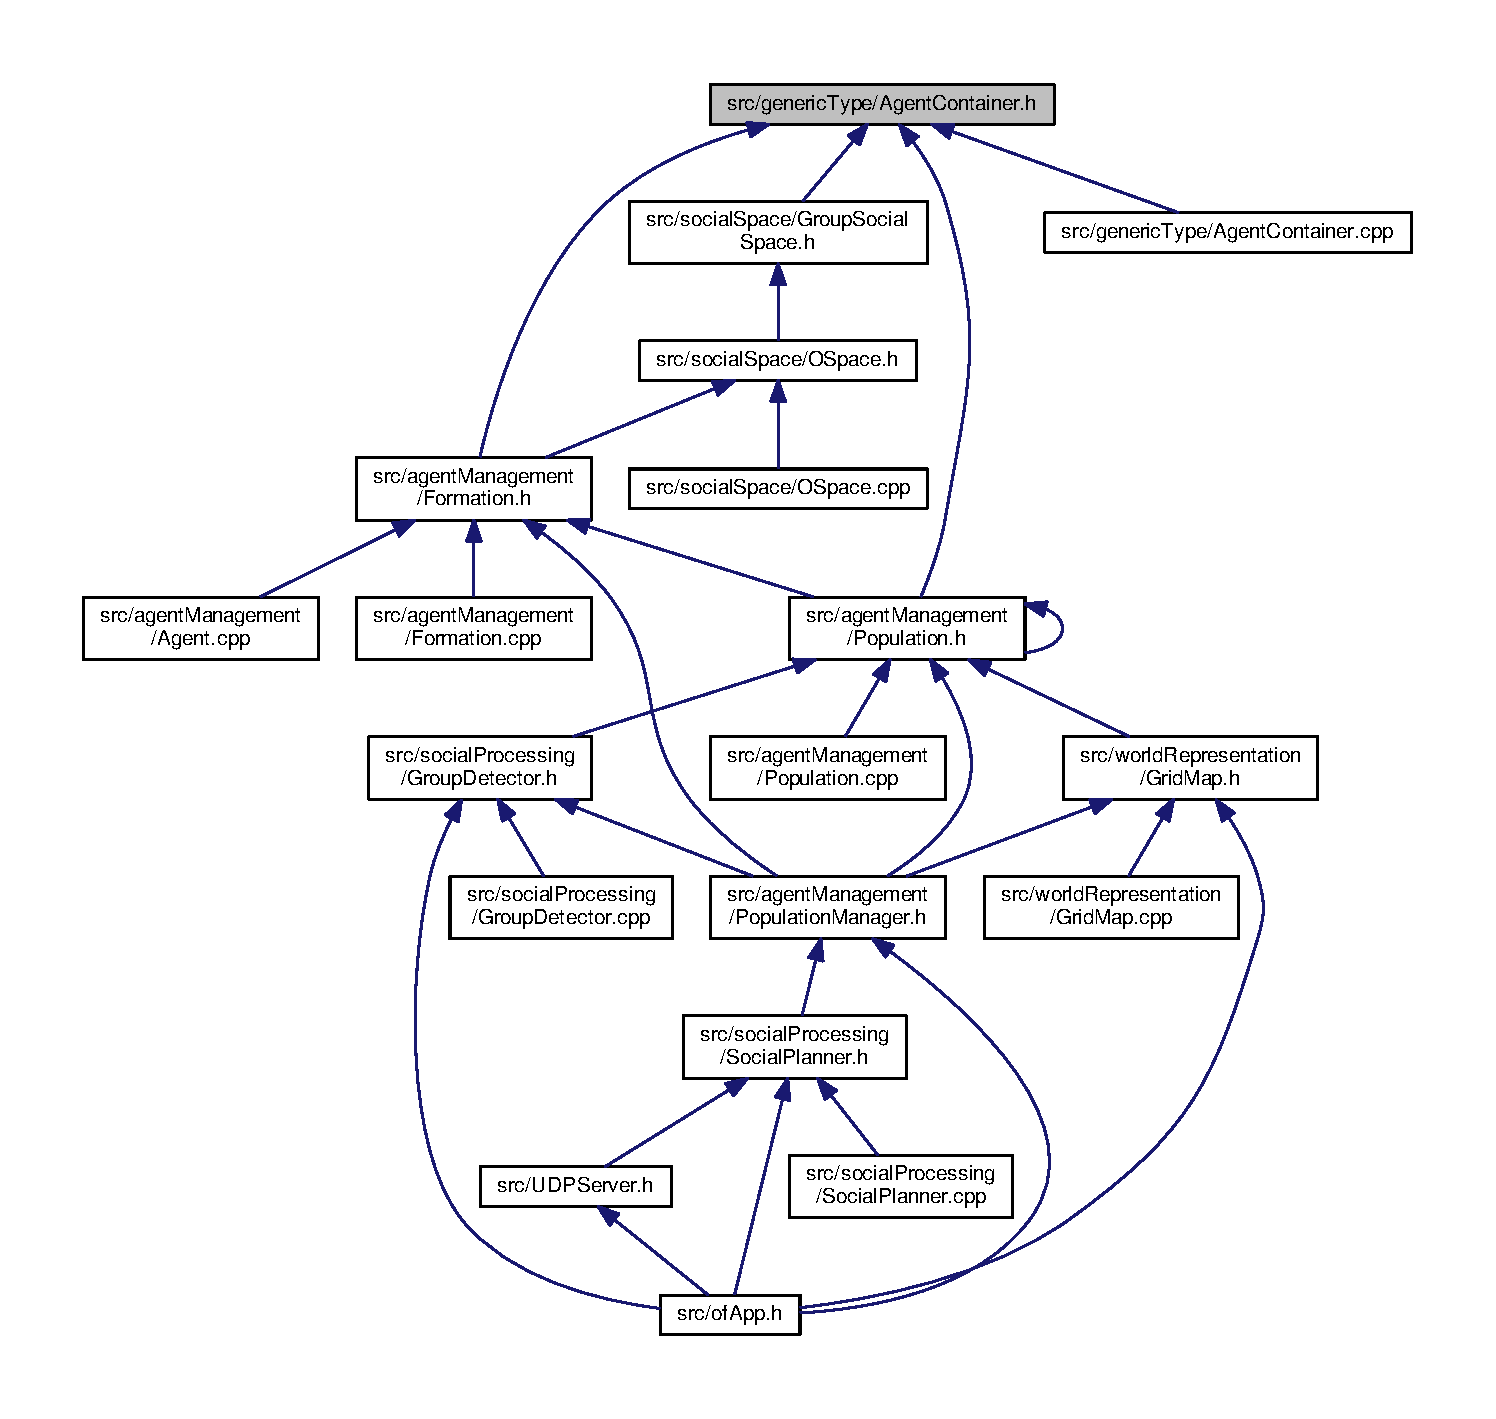
\includegraphics[width=350pt]{AgentContainer_8h__dep__incl}
\end{center}
\end{figure}
\subsection*{Classes}
\begin{DoxyCompactItemize}
\item 
class \hyperlink{classAgentContainer}{Agent\+Container}
\begin{DoxyCompactList}\small\item\em This class is an interface for class that contains multiples Agents. \end{DoxyCompactList}\end{DoxyCompactItemize}


\subsection{Detailed Description}
\begin{DoxyAuthor}{Author}
Paco Dupont 
\end{DoxyAuthor}
\begin{DoxyVersion}{Version}
0.\+1 
\end{DoxyVersion}
\begin{DoxyDate}{Date}
27 mars 2017 
\end{DoxyDate}

\hypertarget{DrawnObject_8cpp}{}\section{src/generic\+Type/\+Drawn\+Object.cpp File Reference}
\label{DrawnObject_8cpp}\index{src/generic\+Type/\+Drawn\+Object.\+cpp@{src/generic\+Type/\+Drawn\+Object.\+cpp}}
{\ttfamily \#include \char`\"{}Drawn\+Object.\+h\char`\"{}}\\*
{\ttfamily \#include \char`\"{}World.\+h\char`\"{}}\\*
{\ttfamily \#include \char`\"{}utils.\+h\char`\"{}}\\*
Include dependency graph for Drawn\+Object.\+cpp\+:\nopagebreak
\begin{figure}[H]
\begin{center}
\leavevmode
\includegraphics[width=350pt]{DrawnObject_8cpp__incl}
\end{center}
\end{figure}


\subsection{Detailed Description}
\begin{DoxyAuthor}{Author}
Paco Dupont 
\end{DoxyAuthor}
\begin{DoxyVersion}{Version}
0.\+1 
\end{DoxyVersion}
\begin{DoxyDate}{Date}
27 mars 2017 
\end{DoxyDate}

\hypertarget{DrawnObject_8h}{}\section{src/generic\+Type/\+Drawn\+Object.h File Reference}
\label{DrawnObject_8h}\index{src/generic\+Type/\+Drawn\+Object.\+h@{src/generic\+Type/\+Drawn\+Object.\+h}}
{\ttfamily \#include \char`\"{}Localized\+Object.\+h\char`\"{}}\\*
Include dependency graph for Drawn\+Object.\+h\+:\nopagebreak
\begin{figure}[H]
\begin{center}
\leavevmode
\includegraphics[width=245pt]{DrawnObject_8h__incl}
\end{center}
\end{figure}
This graph shows which files directly or indirectly include this file\+:\nopagebreak
\begin{figure}[H]
\begin{center}
\leavevmode
\includegraphics[width=350pt]{DrawnObject_8h__dep__incl}
\end{center}
\end{figure}
\subsection*{Classes}
\begin{DoxyCompactItemize}
\item 
class \hyperlink{classDrawnObject}{Drawn\+Object}
\begin{DoxyCompactList}\small\item\em This class is an interface for class that are drawn on O\+FX gui. \end{DoxyCompactList}\end{DoxyCompactItemize}


\subsection{Detailed Description}
\begin{DoxyAuthor}{Author}
Paco Dupont 
\end{DoxyAuthor}
\begin{DoxyVersion}{Version}
0.\+1 
\end{DoxyVersion}
\begin{DoxyDate}{Date}
27 mars 2017 
\end{DoxyDate}

\hypertarget{IdentifiedObject_8cpp}{}\section{src/generic\+Type/\+Identified\+Object.cpp File Reference}
\label{IdentifiedObject_8cpp}\index{src/generic\+Type/\+Identified\+Object.\+cpp@{src/generic\+Type/\+Identified\+Object.\+cpp}}
{\ttfamily \#include \char`\"{}Identified\+Object.\+h\char`\"{}}\\*
Include dependency graph for Identified\+Object.\+cpp\+:\nopagebreak
\begin{figure}[H]
\begin{center}
\leavevmode
\includegraphics[width=209pt]{IdentifiedObject_8cpp__incl}
\end{center}
\end{figure}


\subsection{Detailed Description}
\begin{DoxyAuthor}{Author}
Paco Dupont 
\end{DoxyAuthor}
\begin{DoxyVersion}{Version}
0.\+1 
\end{DoxyVersion}
\begin{DoxyDate}{Date}
27 mars 2017 
\end{DoxyDate}

\hypertarget{IdentifiedObject_8h}{}\section{src/generic\+Type/\+Identified\+Object.h File Reference}
\label{IdentifiedObject_8h}\index{src/generic\+Type/\+Identified\+Object.\+h@{src/generic\+Type/\+Identified\+Object.\+h}}
This graph shows which files directly or indirectly include this file\+:\nopagebreak
\begin{figure}[H]
\begin{center}
\leavevmode
\includegraphics[width=350pt]{IdentifiedObject_8h__dep__incl}
\end{center}
\end{figure}
\subsection*{Classes}
\begin{DoxyCompactItemize}
\item 
class \hyperlink{classIdentifiedObject}{Identified\+Object}
\begin{DoxyCompactList}\small\item\em This class is an interface for class that need a unique identifier. \end{DoxyCompactList}\end{DoxyCompactItemize}


\subsection{Detailed Description}
\begin{DoxyAuthor}{Author}
Paco Dupont 
\end{DoxyAuthor}
\begin{DoxyVersion}{Version}
0.\+1 
\end{DoxyVersion}
\begin{DoxyDate}{Date}
27 mars 2017 
\end{DoxyDate}

\hypertarget{LocalizedObject_8cpp}{}\section{src/generic\+Type/\+Localized\+Object.cpp File Reference}
\label{LocalizedObject_8cpp}\index{src/generic\+Type/\+Localized\+Object.\+cpp@{src/generic\+Type/\+Localized\+Object.\+cpp}}
{\ttfamily \#include \char`\"{}Localized\+Object.\+h\char`\"{}}\\*
Include dependency graph for Localized\+Object.\+cpp\+:\nopagebreak
\begin{figure}[H]
\begin{center}
\leavevmode
\includegraphics[width=233pt]{LocalizedObject_8cpp__incl}
\end{center}
\end{figure}


\subsection{Detailed Description}
\begin{DoxyAuthor}{Author}
Paco Dupont 
\end{DoxyAuthor}
\begin{DoxyVersion}{Version}
0.\+1 
\end{DoxyVersion}
\begin{DoxyDate}{Date}
27 mars 2017 
\end{DoxyDate}

\hypertarget{LocalizedObject_8h}{}\section{src/generic\+Type/\+Localized\+Object.h File Reference}
\label{LocalizedObject_8h}\index{src/generic\+Type/\+Localized\+Object.\+h@{src/generic\+Type/\+Localized\+Object.\+h}}
{\ttfamily \#include \char`\"{}ofx\+Matrix\+Eigen.\+h\char`\"{}}\\*
{\ttfamily \#include $<$cmath$>$}\\*
Include dependency graph for Localized\+Object.\+h\+:\nopagebreak
\begin{figure}[H]
\begin{center}
\leavevmode
\includegraphics[width=233pt]{LocalizedObject_8h__incl}
\end{center}
\end{figure}
This graph shows which files directly or indirectly include this file\+:\nopagebreak
\begin{figure}[H]
\begin{center}
\leavevmode
\includegraphics[width=350pt]{LocalizedObject_8h__dep__incl}
\end{center}
\end{figure}
\subsection*{Classes}
\begin{DoxyCompactItemize}
\item 
class \hyperlink{classLocalizedObject}{Localized\+Object}
\begin{DoxyCompactList}\small\item\em This class is an interface for object that are localized in real \hyperlink{classWorld}{World}. \end{DoxyCompactList}\end{DoxyCompactItemize}


\subsection{Detailed Description}
\begin{DoxyAuthor}{Author}
Paco Dupont 
\end{DoxyAuthor}
\begin{DoxyVersion}{Version}
0.\+1 
\end{DoxyVersion}
\begin{DoxyDate}{Date}
27 mars 2017 
\end{DoxyDate}

\hypertarget{GroupDetector_8cpp}{}\section{src/social\+Processing/\+Group\+Detector.cpp File Reference}
\label{GroupDetector_8cpp}\index{src/social\+Processing/\+Group\+Detector.\+cpp@{src/social\+Processing/\+Group\+Detector.\+cpp}}
{\ttfamily \#include \char`\"{}Group\+Detector.\+h\char`\"{}}\\*
{\ttfamily \#include \char`\"{}utils.\+h\char`\"{}}\\*
{\ttfamily \#include \char`\"{}config.\+h\char`\"{}}\\*
Include dependency graph for Group\+Detector.\+cpp\+:\nopagebreak
\begin{figure}[H]
\begin{center}
\leavevmode
\includegraphics[width=350pt]{GroupDetector_8cpp__incl}
\end{center}
\end{figure}


\subsection{Detailed Description}
\begin{DoxyAuthor}{Author}
Paco Dupont 
\end{DoxyAuthor}
\begin{DoxyVersion}{Version}
0.\+1 
\end{DoxyVersion}
\begin{DoxyDate}{Date}
10 avril 2017 
\end{DoxyDate}

\hypertarget{GroupDetector_8h}{}\section{src/social\+Processing/\+Group\+Detector.h File Reference}
\label{GroupDetector_8h}\index{src/social\+Processing/\+Group\+Detector.\+h@{src/social\+Processing/\+Group\+Detector.\+h}}
{\ttfamily \#include \char`\"{}Population.\+h\char`\"{}}\\*
{\ttfamily \#include \char`\"{}Agent.\+h\char`\"{}}\\*
{\ttfamily \#include \char`\"{}ofx\+Matrix\+Eigen.\+h\char`\"{}}\\*
{\ttfamily \#include $<$cmath$>$}\\*
Include dependency graph for Group\+Detector.\+h\+:\nopagebreak
\begin{figure}[H]
\begin{center}
\leavevmode
\includegraphics[width=350pt]{GroupDetector_8h__incl}
\end{center}
\end{figure}
This graph shows which files directly or indirectly include this file\+:\nopagebreak
\begin{figure}[H]
\begin{center}
\leavevmode
\includegraphics[width=350pt]{GroupDetector_8h__dep__incl}
\end{center}
\end{figure}
\subsection*{Classes}
\begin{DoxyCompactItemize}
\item 
class \hyperlink{classGroupDetector}{Group\+Detector}
\begin{DoxyCompactList}\small\item\em This class is dedicated to process every Agents in the \hyperlink{classPopulation}{Population} and create every \hyperlink{classFormation}{Formation}. \end{DoxyCompactList}\end{DoxyCompactItemize}


\subsection{Detailed Description}
\begin{DoxyAuthor}{Author}
Paco Dupont 
\end{DoxyAuthor}
\begin{DoxyVersion}{Version}
0.\+1 
\end{DoxyVersion}
\begin{DoxyDate}{Date}
10 avril 2017 
\end{DoxyDate}

\hypertarget{SocialPlanner_8cpp}{}\section{src/social\+Processing/\+Social\+Planner.cpp File Reference}
\label{SocialPlanner_8cpp}\index{src/social\+Processing/\+Social\+Planner.\+cpp@{src/social\+Processing/\+Social\+Planner.\+cpp}}
{\ttfamily \#include \char`\"{}Social\+Planner.\+h\char`\"{}}\\*
{\ttfamily \#include \char`\"{}config.\+h\char`\"{}}\\*
{\ttfamily \#include $<$algorithm$>$}\\*
Include dependency graph for Social\+Planner.\+cpp\+:\nopagebreak
\begin{figure}[H]
\begin{center}
\leavevmode
\includegraphics[width=350pt]{SocialPlanner_8cpp__incl}
\end{center}
\end{figure}
\subsection*{Functions}
\begin{DoxyCompactItemize}
\item 
int {\bfseries min\+\_\+2} (int a, int b)\hypertarget{SocialPlanner_8cpp_af4d25f3f1939424ad4be8e5e45c63d06}{}\label{SocialPlanner_8cpp_af4d25f3f1939424ad4be8e5e45c63d06}

\end{DoxyCompactItemize}


\subsection{Detailed Description}
\begin{DoxyAuthor}{Author}
Paco Dupont 
\end{DoxyAuthor}
\begin{DoxyVersion}{Version}
0.\+1 
\end{DoxyVersion}
\begin{DoxyDate}{Date}
7 juin 2017 
\end{DoxyDate}

\hypertarget{SocialPlanner_8h}{}\section{src/social\+Processing/\+Social\+Planner.h File Reference}
\label{SocialPlanner_8h}\index{src/social\+Processing/\+Social\+Planner.\+h@{src/social\+Processing/\+Social\+Planner.\+h}}
{\ttfamily \#include \char`\"{}Population\+Manager.\+h\char`\"{}}\\*
{\ttfamily \#include \char`\"{}Robot.\+h\char`\"{}}\\*
{\ttfamily \#include $<$chrono$>$}\\*
Include dependency graph for Social\+Planner.\+h\+:\nopagebreak
\begin{figure}[H]
\begin{center}
\leavevmode
\includegraphics[width=350pt]{SocialPlanner_8h__incl}
\end{center}
\end{figure}
This graph shows which files directly or indirectly include this file\+:\nopagebreak
\begin{figure}[H]
\begin{center}
\leavevmode
\includegraphics[width=322pt]{SocialPlanner_8h__dep__incl}
\end{center}
\end{figure}
\subsection*{Classes}
\begin{DoxyCompactItemize}
\item 
class \hyperlink{classSocialPlanner}{Social\+Planner}
\begin{DoxyCompactList}\small\item\em This class is a state machine controlling the \hyperlink{classRobot}{Robot} behavior. \end{DoxyCompactList}\end{DoxyCompactItemize}


\subsection{Detailed Description}
\begin{DoxyAuthor}{Author}
Paco Dupont 
\end{DoxyAuthor}
\begin{DoxyVersion}{Version}
0.\+1 
\end{DoxyVersion}
\begin{DoxyDate}{Date}
7 juin 2017 
\end{DoxyDate}

\hypertarget{GaussianSpace_8cpp}{}\section{src/social\+Space/\+Gaussian\+Space.cpp File Reference}
\label{GaussianSpace_8cpp}\index{src/social\+Space/\+Gaussian\+Space.\+cpp@{src/social\+Space/\+Gaussian\+Space.\+cpp}}
{\ttfamily \#include \char`\"{}Gaussian\+Space.\+h\char`\"{}}\\*
{\ttfamily \#include \char`\"{}math.\+h\char`\"{}}\\*
{\ttfamily \#include \char`\"{}utils.\+h\char`\"{}}\\*
Include dependency graph for Gaussian\+Space.\+cpp\+:\nopagebreak
\begin{figure}[H]
\begin{center}
\leavevmode
\includegraphics[width=350pt]{GaussianSpace_8cpp__incl}
\end{center}
\end{figure}


\subsection{Detailed Description}
\begin{DoxyAuthor}{Author}
Paco Dupont 
\end{DoxyAuthor}
\begin{DoxyVersion}{Version}
0.\+1 
\end{DoxyVersion}
\begin{DoxyDate}{Date}
28 mars 2017 
\end{DoxyDate}

\hypertarget{GaussianSpace_8h}{}\section{src/social\+Space/\+Gaussian\+Space.h File Reference}
\label{GaussianSpace_8h}\index{src/social\+Space/\+Gaussian\+Space.\+h@{src/social\+Space/\+Gaussian\+Space.\+h}}
{\ttfamily \#include \char`\"{}Personnal\+Social\+Space.\+h\char`\"{}}\\*
{\ttfamily \#include \char`\"{}ofx\+Matrix\+Eigen.\+h\char`\"{}}\\*
{\ttfamily \#include $<$cmath$>$}\\*
Include dependency graph for Gaussian\+Space.\+h\+:\nopagebreak
\begin{figure}[H]
\begin{center}
\leavevmode
\includegraphics[width=350pt]{GaussianSpace_8h__incl}
\end{center}
\end{figure}
This graph shows which files directly or indirectly include this file\+:\nopagebreak
\begin{figure}[H]
\begin{center}
\leavevmode
\includegraphics[width=350pt]{GaussianSpace_8h__dep__incl}
\end{center}
\end{figure}
\subsection*{Classes}
\begin{DoxyCompactItemize}
\item 
class \hyperlink{classGaussianSpace}{Gaussian\+Space}
\begin{DoxyCompactList}\small\item\em This class is an implementation of the \hyperlink{classPersonnalSocialSpace}{Personnal\+Social\+Space}. \end{DoxyCompactList}\end{DoxyCompactItemize}


\subsection{Detailed Description}
\begin{DoxyAuthor}{Author}
Paco Dupont 
\end{DoxyAuthor}
\begin{DoxyVersion}{Version}
0.\+1 
\end{DoxyVersion}
\begin{DoxyDate}{Date}
28 mars 2017 
\end{DoxyDate}

\hypertarget{GroupSocialSpace_8h}{}\section{src/social\+Space/\+Group\+Social\+Space.h File Reference}
\label{GroupSocialSpace_8h}\index{src/social\+Space/\+Group\+Social\+Space.\+h@{src/social\+Space/\+Group\+Social\+Space.\+h}}
{\ttfamily \#include \char`\"{}Social\+Space.\+h\char`\"{}}\\*
{\ttfamily \#include \char`\"{}Agent\+Container.\+h\char`\"{}}\\*
Include dependency graph for Group\+Social\+Space.\+h\+:\nopagebreak
\begin{figure}[H]
\begin{center}
\leavevmode
\includegraphics[width=343pt]{GroupSocialSpace_8h__incl}
\end{center}
\end{figure}
This graph shows which files directly or indirectly include this file\+:\nopagebreak
\begin{figure}[H]
\begin{center}
\leavevmode
\includegraphics[width=350pt]{GroupSocialSpace_8h__dep__incl}
\end{center}
\end{figure}
\subsection*{Classes}
\begin{DoxyCompactItemize}
\item 
class \hyperlink{classGroupSocialSpace}{Group\+Social\+Space}
\begin{DoxyCompactList}\small\item\em This class is an interface to implement representation of a \hyperlink{classGroupSocialSpace}{Group\+Social\+Space}. \end{DoxyCompactList}\end{DoxyCompactItemize}


\subsection{Detailed Description}
\begin{DoxyAuthor}{Author}
Paco Dupont 
\end{DoxyAuthor}
\begin{DoxyVersion}{Version}
0.\+1 
\end{DoxyVersion}
\begin{DoxyDate}{Date}
29 mars 2017 
\end{DoxyDate}

\hypertarget{OSpace_8cpp}{}\section{src/social\+Space/\+O\+Space.cpp File Reference}
\label{OSpace_8cpp}\index{src/social\+Space/\+O\+Space.\+cpp@{src/social\+Space/\+O\+Space.\+cpp}}
{\ttfamily \#include \char`\"{}O\+Space.\+h\char`\"{}}\\*
{\ttfamily \#include \char`\"{}utils.\+h\char`\"{}}\\*
{\ttfamily \#include \char`\"{}of\+Main.\+h\char`\"{}}\\*
Include dependency graph for O\+Space.\+cpp\+:\nopagebreak
\begin{figure}[H]
\begin{center}
\leavevmode
\includegraphics[width=350pt]{OSpace_8cpp__incl}
\end{center}
\end{figure}


\subsection{Detailed Description}
\begin{DoxyAuthor}{Author}
Paco Dupont 
\end{DoxyAuthor}
\begin{DoxyVersion}{Version}
0.\+1 
\end{DoxyVersion}
\begin{DoxyDate}{Date}
27 mars 2017 
\end{DoxyDate}

\hypertarget{OSpace_8h}{}\section{src/social\+Space/\+O\+Space.h File Reference}
\label{OSpace_8h}\index{src/social\+Space/\+O\+Space.\+h@{src/social\+Space/\+O\+Space.\+h}}
{\ttfamily \#include \char`\"{}Group\+Social\+Space.\+h\char`\"{}}\\*
{\ttfamily \#include \char`\"{}Drawn\+Object.\+h\char`\"{}}\\*
{\ttfamily \#include \char`\"{}config.\+h\char`\"{}}\\*
{\ttfamily \#include \char`\"{}ofx\+Matrix\+Eigen.\+h\char`\"{}}\\*
{\ttfamily \#include $<$cmath$>$}\\*
Include dependency graph for O\+Space.\+h\+:\nopagebreak
\begin{figure}[H]
\begin{center}
\leavevmode
\includegraphics[width=350pt]{OSpace_8h__incl}
\end{center}
\end{figure}
This graph shows which files directly or indirectly include this file\+:\nopagebreak
\begin{figure}[H]
\begin{center}
\leavevmode
\includegraphics[width=350pt]{OSpace_8h__dep__incl}
\end{center}
\end{figure}
\subsection*{Classes}
\begin{DoxyCompactItemize}
\item 
class \hyperlink{classOSpace}{O\+Space}
\begin{DoxyCompactList}\small\item\em This class is an implementation of the \hyperlink{classGroupSocialSpace}{Group\+Social\+Space}. \end{DoxyCompactList}\end{DoxyCompactItemize}


\subsection{Detailed Description}
\begin{DoxyAuthor}{Author}
Paco Dupont 
\end{DoxyAuthor}
\begin{DoxyVersion}{Version}
0.\+1 
\end{DoxyVersion}
\begin{DoxyDate}{Date}
27 mars 2017 
\end{DoxyDate}

\hypertarget{PersonnalSocialSpace_8cpp}{}\section{src/social\+Space/\+Personnal\+Social\+Space.cpp File Reference}
\label{PersonnalSocialSpace_8cpp}\index{src/social\+Space/\+Personnal\+Social\+Space.\+cpp@{src/social\+Space/\+Personnal\+Social\+Space.\+cpp}}
{\ttfamily \#include \char`\"{}Personnal\+Social\+Space.\+h\char`\"{}}\\*
{\ttfamily \#include \char`\"{}Agent.\+h\char`\"{}}\\*
Include dependency graph for Personnal\+Social\+Space.\+cpp\+:\nopagebreak
\begin{figure}[H]
\begin{center}
\leavevmode
\includegraphics[width=346pt]{PersonnalSocialSpace_8cpp__incl}
\end{center}
\end{figure}


\subsection{Detailed Description}
\begin{DoxyAuthor}{Author}
Paco Dupont 
\end{DoxyAuthor}
\begin{DoxyVersion}{Version}
0.\+1 
\end{DoxyVersion}
\begin{DoxyDate}{Date}
29 mars 2017 
\end{DoxyDate}

\hypertarget{PersonnalSocialSpace_8h}{}\section{src/social\+Space/\+Personnal\+Social\+Space.h File Reference}
\label{PersonnalSocialSpace_8h}\index{src/social\+Space/\+Personnal\+Social\+Space.\+h@{src/social\+Space/\+Personnal\+Social\+Space.\+h}}
{\ttfamily \#include \char`\"{}Social\+Space.\+h\char`\"{}}\\*
{\ttfamily \#include \char`\"{}Agent.\+h\char`\"{}}\\*
Include dependency graph for Personnal\+Social\+Space.\+h\+:\nopagebreak
\begin{figure}[H]
\begin{center}
\leavevmode
\includegraphics[width=343pt]{PersonnalSocialSpace_8h__incl}
\end{center}
\end{figure}
This graph shows which files directly or indirectly include this file\+:\nopagebreak
\begin{figure}[H]
\begin{center}
\leavevmode
\includegraphics[width=350pt]{PersonnalSocialSpace_8h__dep__incl}
\end{center}
\end{figure}
\subsection*{Classes}
\begin{DoxyCompactItemize}
\item 
class \hyperlink{classPersonnalSocialSpace}{Personnal\+Social\+Space}
\begin{DoxyCompactList}\small\item\em This class is an interface to implement representation of a \hyperlink{classPersonnalSocialSpace}{Personnal\+Social\+Space}. \end{DoxyCompactList}\end{DoxyCompactItemize}


\subsection{Detailed Description}
\begin{DoxyAuthor}{Author}
Paco Dupont 
\end{DoxyAuthor}
\begin{DoxyVersion}{Version}
0.\+1 
\end{DoxyVersion}
\begin{DoxyDate}{Date}
29 mars 2017 
\end{DoxyDate}

\hypertarget{SocialSpace_8cpp}{}\section{src/social\+Space/\+Social\+Space.cpp File Reference}
\label{SocialSpace_8cpp}\index{src/social\+Space/\+Social\+Space.\+cpp@{src/social\+Space/\+Social\+Space.\+cpp}}
{\ttfamily \#include \char`\"{}Social\+Space.\+h\char`\"{}}\\*
Include dependency graph for Social\+Space.\+cpp\+:\nopagebreak
\begin{figure}[H]
\begin{center}
\leavevmode
\includegraphics[width=243pt]{SocialSpace_8cpp__incl}
\end{center}
\end{figure}


\subsection{Detailed Description}
\begin{DoxyAuthor}{Author}
Paco Dupont 
\end{DoxyAuthor}
\begin{DoxyVersion}{Version}
0.\+1 
\end{DoxyVersion}
\begin{DoxyDate}{Date}
27 mars 2017 
\end{DoxyDate}

\hypertarget{SocialSpace_8h}{}\section{src/social\+Space/\+Social\+Space.h File Reference}
\label{SocialSpace_8h}\index{src/social\+Space/\+Social\+Space.\+h@{src/social\+Space/\+Social\+Space.\+h}}
{\ttfamily \#include \char`\"{}Identified\+Object.\+h\char`\"{}}\\*
Include dependency graph for Social\+Space.\+h\+:\nopagebreak
\begin{figure}[H]
\begin{center}
\leavevmode
\includegraphics[width=232pt]{SocialSpace_8h__incl}
\end{center}
\end{figure}
This graph shows which files directly or indirectly include this file\+:\nopagebreak
\begin{figure}[H]
\begin{center}
\leavevmode
\includegraphics[width=350pt]{SocialSpace_8h__dep__incl}
\end{center}
\end{figure}
\subsection*{Classes}
\begin{DoxyCompactItemize}
\item 
class \hyperlink{classSocialSpace}{Social\+Space}
\begin{DoxyCompactList}\small\item\em This class is an abstract class for representing \hyperlink{classSocialSpace}{Social\+Space}. \end{DoxyCompactList}\end{DoxyCompactItemize}


\subsection{Detailed Description}
\begin{DoxyAuthor}{Author}
Paco Dupont 
\end{DoxyAuthor}
\begin{DoxyVersion}{Version}
0.\+1 
\end{DoxyVersion}
\begin{DoxyDate}{Date}
27 mars 2017 
\end{DoxyDate}

\hypertarget{UDPServer_8h}{}\section{src/\+U\+D\+P\+Server.h File Reference}
\label{UDPServer_8h}\index{src/\+U\+D\+P\+Server.\+h@{src/\+U\+D\+P\+Server.\+h}}
{\ttfamily \#include $<$sys/socket.\+h$>$}\\*
{\ttfamily \#include $<$sys/types.\+h$>$}\\*
{\ttfamily \#include $<$arpa/inet.\+h$>$}\\*
{\ttfamily \#include $<$unistd.\+h$>$}\\*
{\ttfamily \#include \char`\"{}Agent.\+h\char`\"{}}\\*
{\ttfamily \#include \char`\"{}Social\+Planner.\+h\char`\"{}}\\*
Include dependency graph for U\+D\+P\+Server.\+h\+:\nopagebreak
\begin{figure}[H]
\begin{center}
\leavevmode
\includegraphics[width=350pt]{UDPServer_8h__incl}
\end{center}
\end{figure}
This graph shows which files directly or indirectly include this file\+:\nopagebreak
\begin{figure}[H]
\begin{center}
\leavevmode
\includegraphics[width=172pt]{UDPServer_8h__dep__incl}
\end{center}
\end{figure}
\subsection*{Classes}
\begin{DoxyCompactItemize}
\item 
class \hyperlink{classUDPServer}{U\+D\+P\+Server}
\begin{DoxyCompactList}\small\item\em This class manage the U\+DP Server sending computed data to a visualization software and receiving \hyperlink{classAgent}{Agent} data from other sensor sources. \end{DoxyCompactList}\end{DoxyCompactItemize}


\subsection{Detailed Description}
\begin{DoxyAuthor}{Author}
Paco Dupont 
\end{DoxyAuthor}
\begin{DoxyVersion}{Version}
0.\+1 
\end{DoxyVersion}
\begin{DoxyDate}{Date}
19 avril 2017 
\end{DoxyDate}

\hypertarget{GridCell_8cpp}{}\section{src/world\+Representation/\+Grid\+Cell.cpp File Reference}
\label{GridCell_8cpp}\index{src/world\+Representation/\+Grid\+Cell.\+cpp@{src/world\+Representation/\+Grid\+Cell.\+cpp}}
{\ttfamily \#include \char`\"{}Grid\+Cell.\+h\char`\"{}}\\*
{\ttfamily \#include \char`\"{}of\+Main.\+h\char`\"{}}\\*
Include dependency graph for Grid\+Cell.\+cpp\+:\nopagebreak
\begin{figure}[H]
\begin{center}
\leavevmode
\includegraphics[width=350pt]{GridCell_8cpp__incl}
\end{center}
\end{figure}


\subsection{Detailed Description}
\begin{DoxyAuthor}{Author}
Paco Dupont 
\end{DoxyAuthor}
\begin{DoxyVersion}{Version}
0.\+1 
\end{DoxyVersion}
\begin{DoxyDate}{Date}
6 avril 2017 
\end{DoxyDate}

\hypertarget{GridCell_8h}{}\section{src/world\+Representation/\+Grid\+Cell.h File Reference}
\label{GridCell_8h}\index{src/world\+Representation/\+Grid\+Cell.\+h@{src/world\+Representation/\+Grid\+Cell.\+h}}
{\ttfamily \#include \char`\"{}World.\+h\char`\"{}}\\*
{\ttfamily \#include \char`\"{}Identified\+Object.\+h\char`\"{}}\\*
{\ttfamily \#include \char`\"{}Drawn\+Object.\+h\char`\"{}}\\*
Include dependency graph for Grid\+Cell.\+h\+:\nopagebreak
\begin{figure}[H]
\begin{center}
\leavevmode
\includegraphics[width=350pt]{GridCell_8h__incl}
\end{center}
\end{figure}
This graph shows which files directly or indirectly include this file\+:\nopagebreak
\begin{figure}[H]
\begin{center}
\leavevmode
\includegraphics[width=350pt]{GridCell_8h__dep__incl}
\end{center}
\end{figure}
\subsection*{Classes}
\begin{DoxyCompactItemize}
\item 
class \hyperlink{classGridCell}{Grid\+Cell}
\begin{DoxyCompactList}\small\item\em This class represent a cell in the \hyperlink{classGridMap}{Grid\+Map}. \end{DoxyCompactList}\end{DoxyCompactItemize}


\subsection{Detailed Description}
\begin{DoxyAuthor}{Author}
Paco Dupont 
\end{DoxyAuthor}
\begin{DoxyVersion}{Version}
0.\+1 
\end{DoxyVersion}
\begin{DoxyDate}{Date}
6 avril 2017 
\end{DoxyDate}

\hypertarget{GridMap_8cpp}{}\section{src/world\+Representation/\+Grid\+Map.cpp File Reference}
\label{GridMap_8cpp}\index{src/world\+Representation/\+Grid\+Map.\+cpp@{src/world\+Representation/\+Grid\+Map.\+cpp}}
{\ttfamily \#include \char`\"{}Grid\+Map.\+h\char`\"{}}\\*
{\ttfamily \#include \char`\"{}utils.\+h\char`\"{}}\\*
Include dependency graph for Grid\+Map.\+cpp\+:\nopagebreak
\begin{figure}[H]
\begin{center}
\leavevmode
\includegraphics[width=350pt]{GridMap_8cpp__incl}
\end{center}
\end{figure}
\subsection*{Functions}
\begin{DoxyCompactItemize}
\item 
double \hyperlink{GridMap_8cpp_adf050f28ce6e2ae82d60a359d11c3319}{heuristic\+Manhattan\+Cost\+Estimate} (\hyperlink{classGridCell}{Grid\+Cell} $\ast$start, \hyperlink{classGridCell}{Grid\+Cell} $\ast$end)
\begin{DoxyCompactList}\small\item\em Estimate the cost of movement from a \hyperlink{classGridCell}{Grid\+Cell} to another. \end{DoxyCompactList}\item 
double \hyperlink{GridMap_8cpp_ac4876d5bdd3fc7d446133f4ca7942a39}{heuristic\+Diagonal\+Cost\+Estimate} (\hyperlink{classGridCell}{Grid\+Cell} $\ast$start, \hyperlink{classGridCell}{Grid\+Cell} $\ast$end)
\begin{DoxyCompactList}\small\item\em Estimate the cost of movement from a \hyperlink{classGridCell}{Grid\+Cell} to another. \end{DoxyCompactList}\end{DoxyCompactItemize}


\subsection{Detailed Description}
\begin{DoxyAuthor}{Author}
Paco Dupont 
\end{DoxyAuthor}
\begin{DoxyVersion}{Version}
0.\+1 
\end{DoxyVersion}
\begin{DoxyDate}{Date}
6 avril 2017 
\end{DoxyDate}


\subsection{Function Documentation}
\index{Grid\+Map.\+cpp@{Grid\+Map.\+cpp}!heuristic\+Diagonal\+Cost\+Estimate@{heuristic\+Diagonal\+Cost\+Estimate}}
\index{heuristic\+Diagonal\+Cost\+Estimate@{heuristic\+Diagonal\+Cost\+Estimate}!Grid\+Map.\+cpp@{Grid\+Map.\+cpp}}
\subsubsection[{\texorpdfstring{heuristic\+Diagonal\+Cost\+Estimate(\+Grid\+Cell $\ast$start, Grid\+Cell $\ast$end)}{heuristicDiagonalCostEstimate(GridCell *start, GridCell *end)}}]{\setlength{\rightskip}{0pt plus 5cm}double heuristic\+Diagonal\+Cost\+Estimate (
\begin{DoxyParamCaption}
\item[{{\bf Grid\+Cell} $\ast$}]{start, }
\item[{{\bf Grid\+Cell} $\ast$}]{end}
\end{DoxyParamCaption}
)}\hypertarget{GridMap_8cpp_ac4876d5bdd3fc7d446133f4ca7942a39}{}\label{GridMap_8cpp_ac4876d5bdd3fc7d446133f4ca7942a39}


Estimate the cost of movement from a \hyperlink{classGridCell}{Grid\+Cell} to another. 

Estimate the cost of movement from a \hyperlink{classGridCell}{Grid\+Cell} to another with diagonal heuristic. This estimate is better for 8 movement allowed


\begin{DoxyParams}{Parameters}
{\em start} & \+: The starting \hyperlink{classGridCell}{Grid\+Cell} \\
\hline
{\em end} & \+: The target \hyperlink{classGridCell}{Grid\+Cell}\\
\hline
\end{DoxyParams}
\begin{DoxyReturn}{Returns}
The value of the estimated cost 
\end{DoxyReturn}
\index{Grid\+Map.\+cpp@{Grid\+Map.\+cpp}!heuristic\+Manhattan\+Cost\+Estimate@{heuristic\+Manhattan\+Cost\+Estimate}}
\index{heuristic\+Manhattan\+Cost\+Estimate@{heuristic\+Manhattan\+Cost\+Estimate}!Grid\+Map.\+cpp@{Grid\+Map.\+cpp}}
\subsubsection[{\texorpdfstring{heuristic\+Manhattan\+Cost\+Estimate(\+Grid\+Cell $\ast$start, Grid\+Cell $\ast$end)}{heuristicManhattanCostEstimate(GridCell *start, GridCell *end)}}]{\setlength{\rightskip}{0pt plus 5cm}double heuristic\+Manhattan\+Cost\+Estimate (
\begin{DoxyParamCaption}
\item[{{\bf Grid\+Cell} $\ast$}]{start, }
\item[{{\bf Grid\+Cell} $\ast$}]{end}
\end{DoxyParamCaption}
)}\hypertarget{GridMap_8cpp_adf050f28ce6e2ae82d60a359d11c3319}{}\label{GridMap_8cpp_adf050f28ce6e2ae82d60a359d11c3319}


Estimate the cost of movement from a \hyperlink{classGridCell}{Grid\+Cell} to another. 

Estimate the cost of movement from a \hyperlink{classGridCell}{Grid\+Cell} to another with manhattan heuristic. This estimate is better for 4 movement allowed


\begin{DoxyParams}{Parameters}
{\em start} & \+: The starting \hyperlink{classGridCell}{Grid\+Cell} \\
\hline
{\em end} & \+: The target \hyperlink{classGridCell}{Grid\+Cell}\\
\hline
\end{DoxyParams}
\begin{DoxyReturn}{Returns}
The value of the estimated cost 
\end{DoxyReturn}

\hypertarget{GridMap_8h}{}\section{src/world\+Representation/\+Grid\+Map.h File Reference}
\label{GridMap_8h}\index{src/world\+Representation/\+Grid\+Map.\+h@{src/world\+Representation/\+Grid\+Map.\+h}}
{\ttfamily \#include \char`\"{}Grid\+Cell.\+h\char`\"{}}\\*
{\ttfamily \#include \char`\"{}World.\+h\char`\"{}}\\*
{\ttfamily \#include \char`\"{}Population.\+h\char`\"{}}\\*
{\ttfamily \#include \char`\"{}of\+Main.\+h\char`\"{}}\\*
Include dependency graph for Grid\+Map.\+h\+:\nopagebreak
\begin{figure}[H]
\begin{center}
\leavevmode
\includegraphics[width=350pt]{GridMap_8h__incl}
\end{center}
\end{figure}
This graph shows which files directly or indirectly include this file\+:\nopagebreak
\begin{figure}[H]
\begin{center}
\leavevmode
\includegraphics[width=350pt]{GridMap_8h__dep__incl}
\end{center}
\end{figure}
\subsection*{Classes}
\begin{DoxyCompactItemize}
\item 
class \hyperlink{classGridMap}{Grid\+Map}
\begin{DoxyCompactList}\small\item\em This class manage the 2D \hyperlink{classGridMap}{Grid\+Map} computed from the Agents \hyperlink{classSocialSpace}{Social\+Space}. \end{DoxyCompactList}\item 
struct \hyperlink{structGridMap_1_1CompaireVCell}{Grid\+Map\+::\+Compaire\+V\+Cell}
\begin{DoxyCompactList}\small\item\em Define an operator for \hyperlink{classGridCell}{Grid\+Cell} and associated g\+Score comparison for A$\ast$ algorithm. \end{DoxyCompactList}\end{DoxyCompactItemize}


\subsection{Detailed Description}
\begin{DoxyAuthor}{Author}
Paco Dupont 
\end{DoxyAuthor}
\begin{DoxyVersion}{Version}
0.\+1 
\end{DoxyVersion}
\begin{DoxyDate}{Date}
6 avril 2017 
\end{DoxyDate}

\hypertarget{World_8h}{}\section{src/world\+Representation/\+World.h File Reference}
\label{World_8h}\index{src/world\+Representation/\+World.\+h@{src/world\+Representation/\+World.\+h}}
{\ttfamily \#include \char`\"{}Drawn\+Object.\+h\char`\"{}}\\*
{\ttfamily \#include \char`\"{}config.\+h\char`\"{}}\\*
Include dependency graph for World.\+h\+:\nopagebreak
\begin{figure}[H]
\begin{center}
\leavevmode
\includegraphics[width=278pt]{World_8h__incl}
\end{center}
\end{figure}
This graph shows which files directly or indirectly include this file\+:\nopagebreak
\begin{figure}[H]
\begin{center}
\leavevmode
\includegraphics[width=350pt]{World_8h__dep__incl}
\end{center}
\end{figure}
\subsection*{Classes}
\begin{DoxyCompactItemize}
\item 
class \hyperlink{classWorld}{World}
\begin{DoxyCompactList}\small\item\em This class represent the main frame coordinates and its projection in pixels. \end{DoxyCompactList}\end{DoxyCompactItemize}


\subsection{Detailed Description}
\begin{DoxyAuthor}{Author}
Paco Dupont 
\end{DoxyAuthor}
\begin{DoxyVersion}{Version}
0.\+1 
\end{DoxyVersion}
\begin{DoxyDate}{Date}
29 mars 2017 
\end{DoxyDate}

%--- End generated contents ---

% Index
\backmatter
\newpage
\phantomsection
\clearemptydoublepage
\addcontentsline{toc}{chapter}{Index}
\printindex

\end{document}
